%%%%%UDSEENDE%%%%%
%% \documentclass[10.5pt,a4paper,twoside,final,oldfontcommands]{memoir}
%% \documentclass[a4paper,twoside,final,oldfontcommands]{memoir}
\documentclass[a4paper,twoside,final,oldfontcommands]{memoir}
\usepackage[inner=1cm, outer=1cm]{geometry}
\usepackage[utf8]{inputenc}
\usepackage[danish,english]{babel}
\usepackage[T1]{fontenc}
\usepackage{amsmath,epsfig,graphicx,color}
%\usepackage[english,ngerman]{babel}
%\usepackage[latin1]{inputenc}
\usepackage{etoolbox}
%\usepackage{ifthen}
%\usepackage{dsfont}
%\usepackage{shadethm}
%\usepackage{framed}
%\usepackage{pstricks}
%\usepackage{graphics}
%\usepackage{tocbibind}
%\usepackage{showkeys}
%\usepackage{units}
\usepackage{amssymb,latexsym}
%\usepackage{subfigure}
%\usepackage{amsfonts}
%\usepackage{makeidx,showidx}
%\usepackage[sc]{mathpazo}
%\linespread{1.05}
%\usepackage[backref=page]{hyperref}
% \usepackage[colorlinks,citecolor=blue,urlcolor=blue]{hyperref}
\usepackage{hyperref}
\usepackage{caption}
% \usepackage{subcaption}
\hypersetup{
urlcolor=black, 
  menucolor=black, 
  citecolor=blue, 
  anchorcolor=darkgreen, 
  filecolor=black, 
  linkcolor=violet, 
  colorlinks=true,
}

%%%%%PAKKER%%%%%

\usepackage{lmodern,amsmath,amssymb,amsthm,verbatim,listings,mathtools,xcolor,xspace,url,doi,enumerate,soul}
\raggedbottom
\usepackage{pdfpages}
%try
\makeatletter
\let\c@lofdepth\relax
\let\c@lotdepth\relax
\makeatother
\usepackage{subfigure}
%end try


%%%%%MERE UDSEENDE%%%%%
\setlength\beforechapskip{-0.7cm}
\setlength\afterchapskip{1.3cm}
\setsecnumdepth{all} \maxsecnumdepth{all} % laver numre også på alt
\settocdepth{section} \maxtocdepth{section}
\AtEndDocument{\ifnum\value{lastsheet}=1 \thispagestyle{empty} \fi } % Fjerner sidetal ved kun én side
%\lstset{ basicstyle=\ttfamily\footnotesize, showstringspaces=false, extendedchars=true, frame=leftline, breaklines=true, breakindent=0pt, prebreak=\mbox{$\searrow$}, postbreak=\mbox{$\rightarrow$}} %,tabsize=4, language=R, % Opsætning af listings-pakken
%\setlrmarginsandblock{3.75cm}{4.25cm}{*}%original
\setlrmarginsandblock{3.5cm}{4.0cm}{*}%mine
%\setulmarginsandblock{4.25cm}{4.25cm}{*}
\checkandfixthelayout[nearest]
\pagestyle{headings}
\nouppercaseheads 
\makeevenhead{headings}{\thepage}{}{\scshape\leftmark}
\makeoddhead{headings}{\scshape\rightmark}{}{\thepage}
\addtopsmarks{headings}{}{
  \createmark{chapter}{left}{shownumber}{}{.\hspace{0.7em}}
}
\pagestyle{headings}
\pagestyle{headings} % reactivates it



%%%%%FIGURES%%%
\captionnamefont{\bfseries\small}
\captiontitlefont{\small}


%%%THEOREMS%%%
%\newcounter{satz}[chapter]
%\renewcommand{\thesatz}{\arabic{chapter}.\arabic{satz}}

\def\theequation{\thechapter.\arabic{equation}}
\def\tag{\refstepcounter{equation}\leqno }
\def\neqno{\refstepcounter{equation}\leqno(\thechapter.\arabic{equation})}

\newtheorem{lemma}{Lemma}[chapter]
\newtheorem{figur}[lemma]{Figure}
\newtheorem{theorem}[lemma]{Theorem}
\newtheorem{proposition}[lemma]{Proposition}
\newtheorem{definition}[lemma]{Definition}
\newtheorem{corollary}[lemma]{Corollary}
\newtheorem{example}[lemma]{Example}
\newtheorem{exercise}[lemma]{Exercise}
\newtheorem{remark}[lemma]{Remark}
\newtheorem{hypothesis}{Hypothesis}
\newtheorem{fig}[lemma]{Figure}
\newtheorem{tab}[lemma]{Table}
\newtheorem{conjecture}[lemma]{Conjecture}

\newcommand{\ble}{\begin{lemma}}
\newcommand{\ele}{\end{lemma}}
\newcommand{\bth}{\begin{theorem}}
\newcommand{\ethe}{\end{theorem}}
\newcommand{\bre}{\begin{remark}\em }
\newcommand{\ere}{\end{remark}}

%% \newtoggle{theoremdefs}
%% \togglefalse{theoremdefs}

%%%%%BIBTEX%%%%%
%\usepackage{natbib}
\bibliographystyle{acm}


%%%%% OWN COMMANDS
\newcommand{\ov}{\overline}
\newcommand{\un}{\underline}

\newcommand{\bfx}{{\bf x}}
\newcommand{\bfs}{{\bf s}}
\newcommand{\bft}{{\bf t}}

\newcommand{\rep}{representation}
\renewcommand{\H}{{\mathbf H}}
\newcommand{\wt }{\widetilde}
\newcommand{\wh }{\widehat}
\newcommand{\pro}{probabilit}
\newcommand{\ld}{large deviation}
\newcommand{\bfw}{{\mathbf w}}
\newcommand{\bfW}{{\mathbf W}}
\newcommand{\bfv}{{\mathbf v}}
\newcommand{\bfA}{{\mathbf A}}
\newcommand{\bfT}{{\mathbf T}}
\newcommand{\bfR}{{\mathbf R}}
\newcommand{\bfD}{{\mathbf D}}
\newcommand{\bfN}{{\mathbf N}}
\newcommand{\bfM}{{\mathbf M}}
\newcommand{\bfF}{{\mathbf F}}
\newcommand{\bfH}{{\mathbf H}}
\newcommand{\bfP}{{\mathbf P}}
\newcommand{\bfQ}{{\mathbf Q}}
\newcommand{\bfI}{{\mathbf I}}
\newcommand{\bfV}{{\mathbf V}}
\newcommand{\bfX}{{\mathbf X}}
\newcommand{\bfY}{{\mathbf Y}}
\newcommand{\bfu}{{\mathbf u}}
\newcommand{\bfQr}{{\mathbf Q}^\rightarrow}
\newcommand{\bfQrm}{{\mathbf Q}^{\rightarrow,(m)}}
\newcommand{\bfQd}{{\mathbf Q}^\downarrow}
\newcommand{\bfQdm}{{\mathbf Q}^{\downarrow,(m)}}
\newcommand{\cmt}{continuous mapping theorem}
\newcommand{\fct}{function}
\newcommand{\slvary}{slowly varying}
\newcommand{\regvar}{regular variation}
\newcommand{\regvary}{regularly varying}
\newcommand{\sth}{such that}
\newcommand{\stas}{\stackrel{\rm a.s.}{\rightarrow}}
\newcommand{\std}{\stackrel{\rm d}{\rightarrow}}
\newcommand{\stp}{\stackrel{\P}{\rightarrow}}
\newcommand{\la}{\lambda}
\newcommand{\ds}{distribution}
\newcommand{\beao}{\begin{eqnarray*}}
\newcommand{\eeao}{\end{eqnarray*}}
\newcommand{\beam}{\begin{eqnarray}}
\newcommand{\eeam}{\end{eqnarray}}
\newcommand{\red}{\color{darkred}}
\newcommand{\blue}{\color{darkblue}}
\newcommand{\green}{\color{darkgreen}}
\newcommand{\black}{\color{black}}
\definecolor{darkblue}{rgb}{.1, 0.1,.8}
\definecolor{darkgreen}{rgb}{0,0.8,0.2}
\definecolor{darkred}{rgb}{.8, .1,.1}
\newcommand{\bco}{\begin{corrolary}}
\newcommand{\eco}{\end{corrolary}}
\newcommand{\wrt}{with respect to}
\newcommand{\R}{\mathbb{R}}
\newcommand{\N}{\mathbb{N}}
\newcommand{\C}{\mathbb{C}}
\newcommand{\bfC}{{\mathbf C}}
\newcommand{\bfB}{{\mathbf B}}
\newcommand{\Z}{\mathbb{Z}}
\newcommand{\Var}{\operatorname{Var}}
\newcommand{\Fo}{\bar{F}}
\renewcommand{\b}[1]{\boldsymbol{#1}}
\newcommand{\Rq}{\mkern 1.5mu\overline{\mkern-1.5mu\R\mkern-3.0mu}\mkern 1.5mu}
\newcommand{\Frechet}{Fr\'{e}chet }
\renewcommand{\Finv}{F^{\gets}}
\DeclareMathOperator{\e}{e}
\newcommand{\inv}[1]{#1^{\gets}}
\newcommand{\x}{{\mathbf x}}
\newcommand{\y}{{\mathbf y}}
\newcommand{\X}{{\mathbf X}}
\newcommand{\Y}{{\mathbf Y}}
\newcommand{\A}{{\mathbf A}}
\newcommand{\bfS}{{\mathbf S}}
\newcommand{\bfZ}{{\mathbf Z}}
\newcommand{\z}{{\mathbf Z}}
\newcommand{\zz}{{\mathbf Z \mathbf Z}'}
\newcommand{\0}{\boldsymbol{0}}
\newcommand{\dint}{\,\mathrm{d}}
\newcommand{\mB}{\mathcal{B}}
\newcommand{\norm}[1]{\|#1\|}
\newcommand{\twonorm}[1]{\|#1\|_2}
\newcommand{\inftynorm}[1]{\|#1\|_\infty}
\newcommand{\frobnorm}[1]{\|#1\|_F}
\newcommand{\ltwonorm}[1]{\|#1\|_{\ell_2}}
\newcommand{\vep}{\varepsilon}
\newcommand{\nto}{n \to \infty}
\newcommand{\xto}{x \to \infty}
\newcommand{\lhs}{left-hand side}
\newcommand{\rhs}{right-hand side}
\newcommand{\ts}{time series}
\newcommand{\tsa}{\ts\ analysis}
\newcommand{\fidi}{finite-dimensional distribution}
\newcommand{\rv}{random variable}
\newcommand{\Zbar}{\overline{Z}}
\newcommand{\Dr}{D^{\rightarrow}}
\newcommand{\Dc}{D^{\downarrow}}
\newcommand{\bfe}{{\mathbf e}}
\newcommand{\MP}{Mar\v cenko--Pastur }
\newcommand{\runs}{\operatorname{runs}}
\newcommand{\length}{\operatorname{length}}

\newcommand{\levy}{L\'evy}
\newcommand{\slln}{strong law of large numbers}
\newcommand{\clt}{central limit theorem}
\newcommand{\sde}{stochastic differential equation}
\newcommand{\It}{It\^o}
\newcommand{\sta}{St\u aric\u a}
\newcommand{\ex}{{\rm e}\,}

\newcommand{\cid}{\stackrel{\rm d}{\rightarrow}}
\newcommand{\cip}{\stackrel{\P}{\rightarrow}}
\newcommand{\civ}{\stackrel{\rm v}{\rightarrow}}
\newcommand{\cas}{\stackrel{\rm a.s.}{\rightarrow}}
\newcommand{\simsl}{\stackrel{sl.}{\sim}}
\newcommand{\eid}{\stackrel{\rm d}{=}}

\newcommand{\med}{{\rm med}}
\newcommand{\corr}{{\rm corr}}
\newcommand{\as}{{\rm a.s.}}
\newcommand{\io}{{\rm i.o.}}
\newcommand{\Holder}{H\"older}
\newcommand{\evt}{extreme value theory}
\newcommand{\cadlag}{c\`adl\`ag}
\newcommand{\pp}{point process}
\newcommand{\con}{convergence}
\newcommand{\seq}{sequence}
\newcommand{\ms}{measure}
\newcommand{\asy}{asymptotic}

\newcommand{\bbr}{{\mathbb R}}
\newcommand{\bbm}{{\mathcal M}}
\newcommand{\bbb}{{\mathcal B}}
\newcommand{\bbz}{{\mathbb Z}}
\newcommand{\bbn}{{\mathbb N}}
\newcommand{\bbd}{{\mathbb D}}
\newcommand{\bbf}{{\mathcal F}}
\newcommand{\bbs}{{\mathbb S}}
\newcommand{\bbE}{{\mathcal E}}

\newcommand{\barr}{\begin{array}}
\newcommand{\earr}{\end{array}}

\newcommand{\fif}{if and only if}
\newcommand{\pd}{\partial}

\usepackage{amssymb,amsmath,amsthm,amsfonts}
\usepackage{mathrsfs}
\usepackage{dsfont}
\usepackage{enumerate}

%\newtheorem{mdef}{Definition}
%\newtheorem{theorem}{Theorem}
\newcommand{\eqsplit}[2]{
  \begin{equation}\label{#2}
    \begin{split}
      #1
    \end{split}
  \end{equation}}
\newcommand{\eqnsplit}[1]{
  \begin{eqnarray*}
    #1
  \end{eqnarray*}}
\newcommand{\tran}[1]{
  \tilde{#1}
}
\newcommand{\td}[2]{
  \frac{d #1}{d #2}
}
\newcommand{\pd}[2]{
  \frac{\partial #1}{\partial #2}
}
\newcommand{\ppd}[2]{
  \frac{\partial^2 #1}{\partial #2^2}
}
\newcommand{\pdd}[3]{
  \frac{\partial^2 #1}{\partial #2 \partial #3}
}
\newcommand{\otd}[1]{
  \frac{d}{d #1}
}
\newcommand{\opd}[1]{
  \frac{\partial}{\partial #1}
}
\newcommand{\oppd}[1]{
  \frac{\partial^2}{\partial #1^2}
}
\newcommand{\opdd}[2]{
  \frac{\partial^2}{\partial #1 \partial #2}
}
\newcommand{\ket}[1]{
  |#1\rangle
}
\newcommand{\bra}[1]{
  \langle#1|
}
\newcommand{\inn}[1]{
  \langle#1\rangle
}
\newcommand{\mean}[1]{
  \langle#1\rangle
}
\newcommand{\tr}{
  \text{tr}\,
}
\newcommand{\re}{
  \text{Re}\,
}
\newcommand\im{
  \text{Im}\,
}
\newcommand{\var}{
  \text{var}
}
\newcommand{\arcsinh}{
  \sinh^{-1}
}
\newcommand{\arccosh}{
  \cosh^{-1}
}
\newcommand{\erfc}{
  \text{erfc}
}
\newcommand{\E}{
  \mathbb{E}
}
\renewcommand{\P}{
  \mathbb{P}
}
\newcommand{\I}[1]{
  \mathbf{1}_{\{#1\}}
}
\newcommand{\1}[1]{
  \mathds{1}_{\{#1\}}
}
\newcommand{\diag}{
  \text{diag\,}
}
\newcommand{\M}{
  {\text{max}}
}
\newcommand{\m}{
  {\text{min}}
}
\newcommand{\ph}{
  {\text{arg}\,}
}
\newcommand\erf{
  \text{erf}
}
\renewcommand\vec[1]{
  \mathbf{#1}
}
\newcommand\mtx[1]{
  \mathbf{#1}
}
\newcommand\ed{
  \,{\buildrel d \over =}\,
}




\usepackage[numbers,sort&compress]{natbib}
\usepackage{algorithm}
\usepackage{algpseudocode}
\usepackage{appendix}
\graphicspath{
        {../papers/FX/}{../papers/Jeffrey1/}
        {../papers/Anja/}
        {../papers/DavisMikoschHeinyXie/}
}



\begin{document}



\frontmatter


\title{\textbf{\HUGE Analysis of Heavy-Tailed Time Series\ \\ \vspace{1.5em}}}	
\author{\Huge \textsc{Xiaolei Xie}}
\date{}
\maketitle
\thispagestyle{empty}
\begin{center}
\LARGE
\Huge\textbf{PhD Thesis}

\vspace{7em}
\LARGE
This thesis has been submitted to the PhD School of the Faculty of Science, University of Copenhagen

\vspace{2em}

Augest 21, 2017

\vspace{2em}

\textsc{Department of Mathematical Sciences \\ Faculty of Science \\ University of Copenhagen}
\end{center}


\newpage
\leavevmode\thispagestyle{empty} 

%\vspace*{1cm}
\hspace*{0.5cm}  {\bf Xiaolei Xie}\\
\hspace*{1.5cm} Department of Mathematical Sciences\\
\hspace*{1.5cm} University of Copenhagen\\
\hspace*{1.5cm} Universitetsparken 5\\
\hspace*{1.5cm} 2100 København Ø\\
\hspace*{1.5cm} Denmark\\
\hspace*{1.5cm} xie@math.ku.dk\\
\hspace*{1.5cm} xie.xiaolei@gmail.com

\vspace*{3cm}

\begin{tabular}{ll}
Supervisor: & Prof.~Thomas Mikosch\\
& University of Copenhagen\\
& \\
Co-supervisor: & Associate Prof.~Jeffrey Collamore\\
& University of Copenhagen\\
& \\
Assessment committee: &  Prof.~Catalin St{\u{a}}ric{\u{a}}\\
& University of Neuchatel, CH\\
& \\

& Prof.~Olivier Wintenberger\\
& University of Marie \& Pierre Curie, Paris\\
& \\

& Lecturer.~Jesper Lund Pedersen (chairman)\\
& University of Copenhagen\\
\end{tabular}

\vspace*{5cm}
\noindent \hspace*{0.5cm} Copyright:\\
\hspace*{0.5cm} Chapters 1-4: \copyright Johannes Heiny (according to Danish legislation)\\
\hspace*{0.5cm} Chapter 2: \copyright Elsevier\\

\noindent \hspace*{0.5cm} ISBN: $978$-$87$-$7078$-$921$-$9$

\begin{comment}
{	\pagestyle{empty}
	\setlength{\topmargin}{0pt}
	\setlength{\headheight}{0pt}
	\setlength{\headsep}{0pt}
	\setlength{\footskip}{0pt}
	
	\setlength{\parskip}{12pt}	
	
	%\begin{center}
		%\vspace*{2.5cm}
 \large \textbf{\textsc{Johannes Heiny}}
		
		\vspace*{1cm}
		
	%\end{center}
	
	\vspace*{\fill}}
\end{comment}


\chapter*{}
\vspace*{-2cm}
\section*{Abstract}
\addcontentsline{toc}{section}{Abstract}

This thesis is about heavy-tailed time series.


\section*{Resum{\'e}}

\newpage
\section*{Acknowledgments}
\addcontentsline{toc}{section}{Acknowledgments}

I owe my gratitude to many people and especially to my supervisors Prof. Mikosch and Prof. Collamore.
\bigskip


{\em Xie Xiaolei\qquad \qquad \qquad \qquad \qquad Copenhagen, September $2017$.}


\chapter*{Summary}
\addcontentsline{toc}{section}{Summary}
This PhD thesis provides results from analysis of heavy-tailed time
series. Its main part consists of the following research papers
written between October $2014$ and Augest $2017$.


\begin{enumerate}
\bibitem[P2]{davis:mikosch:heiny:xie:20151}
{\sc Davis, R.~A., Heiny, J., Mikosch, T., and Xie, X.}
\newblock Extreme value analysis for the sample autocovariance matrices of
  heavy-tailed multivariate time series.
\newblock {\em Extremes 19}, 3 (2016), 517--547. \href{http://link.springer.com/article/10.1007/s10687-016-0251-7}{\blue{[pdf]}}
\end{enumerate}

Now we explain the structure of this thesis.

{\em Xie Xiaolei \qquad \qquad \qquad \qquad \qquad Copenhagen, January $2017$.}

\newpage
\tableofcontents

\mainmatter

\def\phdthesis{1}
\chapter{Introduction}\label{ch:intr}
The phenomena of heavy-tailedness is widely observed in many
disciplines of science, for example, phase transition of matter and
black body radiation as studied in physics, neuronal avalanches in
biology, claim sizes of insurance mathematics and stock returns in
finance. The last application is indeed the focus of this thesis. To
discuss the phenomena in precise terms, we introduce the concept of
regular variation.

\section{Regular Variation}
The concept of regular variation is defined by the following scaling
property: if a function $f(\cdot)$ satisfies
\[
\lim_{x \to \infty} {f(c x) \over f(x)} = c^\alpha
\quad
\forall c > 0
\]
then we say $f(x)$ is regularly varying with index $\alpha$.
% Distribution functions, say $F(\cdot)$, whose survival function
% $\bar F(x) = 1 - F(x)$ satisfies the above scaling property, are
% observed in a variety of phenomena, 
When expanded to multiple dimensions, the scaling property of regular
variation is better described in terms of vague convergence to a
spectral measure $\mu_\alpha$: if a random vector $V$ satisfies
\[
{
  \P(V/|V| \in \cdot, |V| > c x)
  \over
  \P(|V| > x)
},
\overset{v}{\to} c^{-\alpha} \mu_\alpha(\cdot)
\quad
x \to \infty, \forall c > 0
\]
then we say the $V$ is regularly varying with index $\alpha$. Here
$\mu_\alpha(\cdot)$ is a probability measure on the unit sphere
\cite{buraczewski:damek:mikosch:2016}. Clearly, if $V$
is regularly varying with index $\alpha$, then each component
of it and each linear combination of its components are regularly
varying with the same index $\alpha$. This follows from Feller
\cite{feller}, p. 278. Cf. also Jessen and Mikosch
\cite{JessenMikosch2006}, lemma 3.1, and Embrechts et. al.
\cite{embrechts:klueppelberg:mikosch:1997}, lemma 1.3.1.

Clearly, estimating the tail index $\alpha$ is particularly important
for understanding the behaviour of a heavy-tailed series. A standard
method proposed for this purpose is due to Hill \cite{hill1975simple}:
\[
\hat \alpha_H = \left[
  {1 \over k} \sum_{i=1}^k \log \left(
  X_{(i)} \over X_{(k+1)}
  \right)
  \right]^{-1}
\]
where $X_1, X_2, \dots$ is the series whose tail index is the subject
of estimation, and $X_{(i)}$ is the $i$-th upper order statistics of
this series. Several authors have contributed to showing the
weak consistency of the estimator $\hat \alpha_H$,
i.e. if $k \to \infty, k/n \to 0$ as $n \to \infty$, then
$\hat \alpha_H \overset{P}{\to} \alpha$.

Mason \cite{mason:1982} first proved that the estimator
was consistent when $X_1, X_2, \dots$ were iid; later Rootz\'en,
Leadbetter and de Haan \cite{rootzen:leadbetter:dehaan1992} and Hsing
\cite{hsing:1991} proved its consistency when $X_1, X_2, \dots$ were
weakly dependent; and Resnick and St{\u a}ric{\u a}
\cite{resnick:starica:1995, resnick:starica:1997} proved its
consistency when $X_t$ was a linear process.

Figure \ref{fig:thjyuj} shows the Hill estimates of the tail indices
of daily stock return series from 3 sectors of the
{\em Standard \& Poor 500} index \footnote{An American stock index
  comprising 500 or so companies.}. The 2.5\% and 97.5\% quantiles of
the asymptotic normal distribution of the estimates are also
given. One can see the confidence bands are fairly large compared with
the estimated values. This certainly raises the question of how
similar they really are and if/how their variations can be explained by
economical arguments. We explore this topic in chapter
\ref{ch:TailParameters}.

\begin{figure}[htb!]
  \begin{minipage}{1.0\linewidth}
    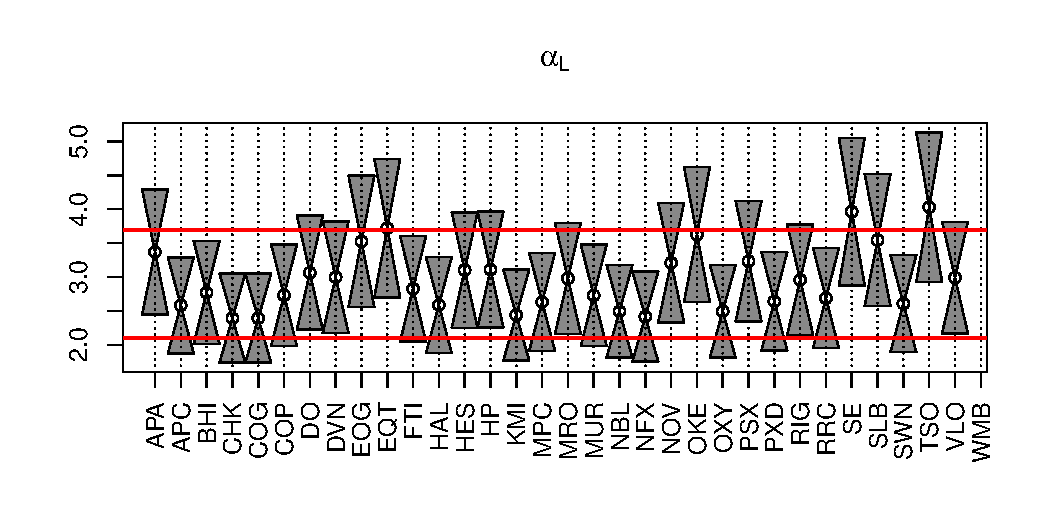
\includegraphics[width=\textwidth, trim={0, 0.8cm, 0, 2cm}, clip]
    {Energy_lower.pdf}
  \end{minipage}
  \begin{minipage}{1.0\linewidth}
    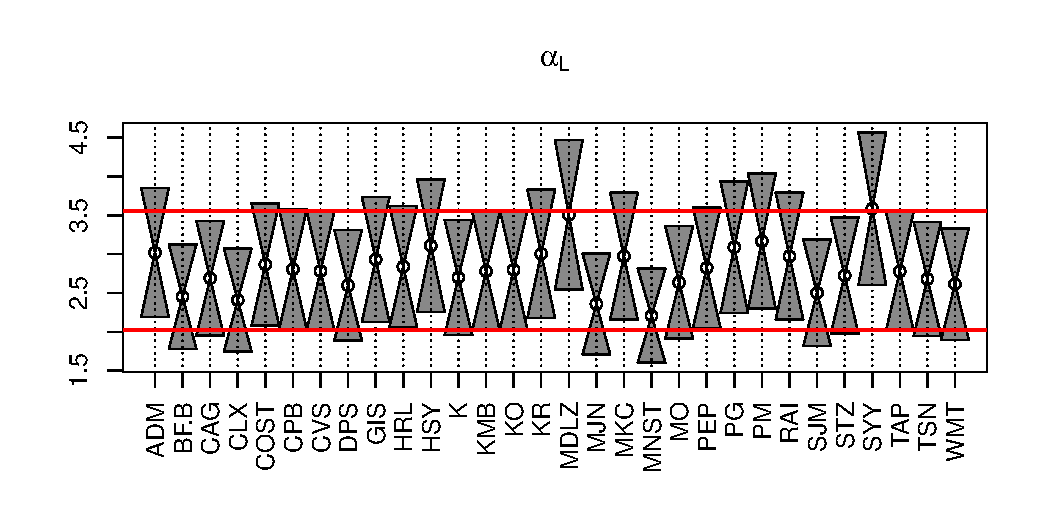
\includegraphics[width=\textwidth, trim={0, 0.8cm, 0, 2cm}, clip]
    {Consumer_Staples_lower.pdf}
  \end{minipage}
  \begin{minipage}{1.0\linewidth}
    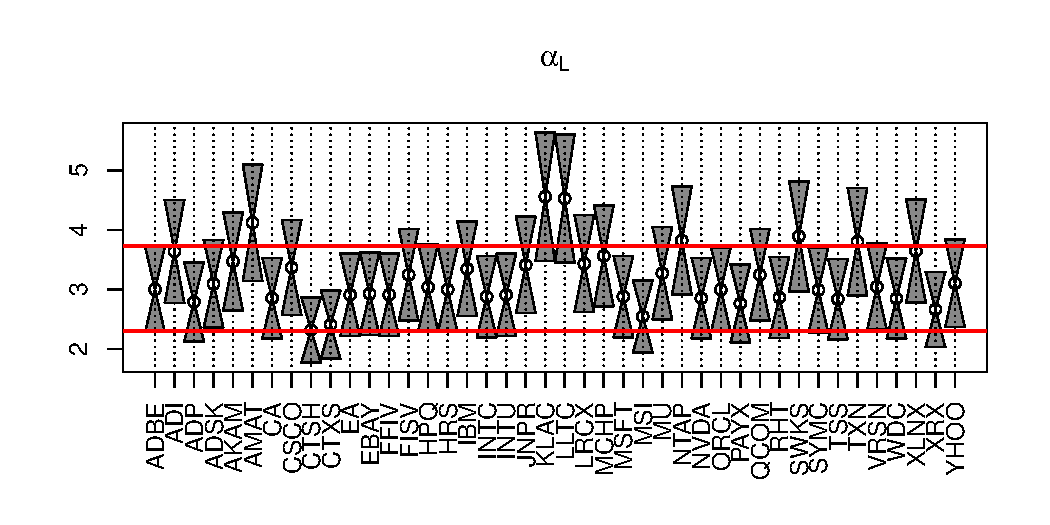
\includegraphics[width=\textwidth, trim={0, 0.8cm, 0, 2cm}, clip]
    {Information_Technology_lower.pdf}
  \end{minipage}
  \caption{\small Hill estimates $\hat \alpha_{50}$ of the lower
    tail-indices $\alpha$ of daily return series in sectors of the S\&P 500
    index. The data span from 1 January 2010 to 31 December 2014 and
    comprise $n=1304$ observations.
    The graphs from top to bottom correspond to the ``Energy'',
    ``Consumer Staples'' and ``Information Technology'' sectors.
    Each circle corresponds to a Hill estimate $\hat\alpha_{50}$; the gray
    triangles above and below it mark the 97.5\% and 2.5\% quantiles
    of its approximate normal distribution; see \eqref{eq:2} and the
    discussion following it for an interpretation.
    The lower and upper red lines mark the medians of the 2.5\% 
    and 97.5\% quantiles, respectively, evaluated from all stocks in
    the sector.
    The data are taken from {\it Yahoo Finance}; the labels on
    the horizontal axes are Yahoo symbols of the stocks. 
  }\label{fig:thjyuj}
\end{figure}

Random variables with regularly varying tails have some very nice
features: if $X_1$ and $X_2$ are both regularly varying with indices
$\alpha_1$ and $\alpha_2$, respectively, then $a_1 X_1 + a_2 X_2$ is
regularly varying with index $\min\{\alpha_1, \alpha_2\}$. Moreover
if $X_1, X_2$ are iid,
$\P(a_1 X_1 + a_2 X_2 > u) \sim \P(a_1 X_1 > u) + \P(a_2 X_2 > u)$.

Now consider $N$ return series $X_{i,t}$, $i=1,2,\dots, p$. Suppose
each of these series is a linear combination of $K$ factors $Y_{i,t}$,
$i=1,2,\dots,K$, the $i$-th of which is regularly varying with index
$\alpha_i$. Then by the summation property, each and every $X_i$ is
regularly varying with index $\min_{1 \leq i \leq K} \alpha_i$.
Since in practice a factor $Y_{i,t}$ is found as a linear combination
of $X_{i,t}$, the observed time series, following an eigenvector of
the sample covariance matrix of $X_{i,t}$, it is important to
understand the eigensystem of this matrix. This topic indeed
constitutes chapters \ref{ch:bernoulli} and \ref{ch:extremes} of this
thesis.

When a product of random variables, say $X_1 X_2$, involves a random
variable with regularly varying tails, a useful result is that of
Breiman: assume $X_1$ is regularly varying with index $\alpha$ and
there exists $\epsilon > 0$ such that
$\E |X_2|^{\alpha + \epsilon} < \infty$.
Then $\P(X_1 X_2 > x) \sim \E|X_2|^{\alpha} \P(X_1 > x)$.
More generally, if $X_1, X_2$ are regularly varying with the same tail
index $\alpha$ or if $\P(X_2 > x) = o(\P(X_1 > x))$, then $X_1 X_2$ is
regularly varying with index $\alpha$.

For an extensive summary of the regular variation properties of
functions of regularly varying random variables, see Mikosch and
Jessen \cite{JessenMikosch2006}.

% When considered as the multiplicative inverse of the parameter of the
% {\em Generalized Extreme Value} distribution, there are other methods
% in the literature for estimating the tail index, e.g. Pickand's 
% estimator \cite{pickands1975statistical} $\hat \alpha_P$ and the
% Deckers-Einmahl-de Haan estimator $\hat \alpha_{\text{DEH}}$
% \begin{eqnarray*}
% {1 \over \hat \alpha_P}
% &=&
% {1 \over \log 2}
% \log {
%   X_{(k)} - X_{(2k)}
%   \over
% X_{(2k)} - X_{(4k)}  
% } \\
% {1 \over \hat \alpha_{\text{DEH}}}
% &=&
% 1 + {1 \over \alpha_H} + {1 \over 2} \left(
%   {H \over \alpha_H^2} - 1
% \right)^{-1}
% \end{eqnarray*}
% where it is similarly assumed $k \to \infty$ and $k/n \to 0$ as $n \to
% \infty$. The Deckers-Einmahl-de Haan estimator makes use of Hill's
% estimator $\hat \alpha_H$ and computes
% \[
% H = \left[
%   {1 \over k} \sum_{i=1}^k \log \left(
%     { X_{(i)} \over X_{(k+1)} }
%   \right)^2
% \right]^{-1}
% \]
% Apparently $1/H$ can be interpreted as the 2nd empirical moment of
% $\log(X_{(i)}/X_{(k+1)})$ for $i \leq k$.
% A major drawback of Pickand's and Deckers-Einmahl-de Haan's estimators
% is that, when applied to estimating the tail index, they discard the
% information that the tail index is always positive, hence resulting in
% a larger confidence band compared with that obtained for Hill's
% estimator. Therefore we stick to Hill's estimator in the empirical
% work included in this thesis.

\section{Stochastic Recurrence Equation}
One of the most important dynamical mechanisms that lead to regularly
varying r.v. is stochastic recursion of the following form:
\begin{equation}
  \label{eq:rhjyu}
  X_t = A_t X_{t-1} + B_t
\end{equation}
where $X_t$ is a $d$-dimensional random vector, $A_t$ is a $d\times d$
random matrix and $B_t$ is a $d$-dimensional vector, random or
deterministic. The sequence $\{A_i\}_{i=1,2,\dots}$ and
$\{B_i\}_{i=1,2,\dots}$  are iid and independent of each other.

Kesten \cite{kesten:1973} showed that, when $A_t$ are almost
surely non-negative, has no row or column of only zeros, and
$B_t$ is almost surely non-negative and is not equal to the null
vector with probability 1, then the strictly stationary solution to
the equation $V \overset{d}{=} A V + B$ has power-law tails
for its marginal distributions, assuming the following conditions (M)
and (A):
\begin{itemize}
\item Condition (M)
  \begin{enumerate}
  \item The top Lyapunov exponent
    \[
    \gamma = \inf_{n \geq 1} {1 \over n}\E \log \|A_n \cdots A_1\|
    \]
    is negative.
  \item There exists $\xi > 0$ such that
    \[
    1 = \lambda(\xi) = \lim_{n \to \infty} {1 \over n} \log \E \|A_n \cdots A_1\|^\xi
    \]
  \item $\E (\|A_1\|^\xi \log^+\|A_1\|) < \infty$
  \item $\E |B_1|^\xi < \infty$
  \end{enumerate}
\item Condition (A) : The group generated by
  \[
  \{\log\rho(s): s = A_n \cdots A_1 \text{ for some } n \geq 1\}
  \]
  is dense in $\reals$, where $\rho(s)$ denotes the spectral
  radius of matrix $s$.
\end{itemize}
Upon these conditions, Kesten's theorem gives
\begin{equation*}
  u^\xi \P(u^{-1} V \in \cdot) \overset{v}{\to} \mu_\xi(\cdot)
\end{equation*}
where $\mu_\xi$ is a non-null Radon measure on
$\reals^d_+ \setminus \{0\}$ with the property
$\mu_\xi(a A) = a^{-\xi} \mu_\xi(A)$.

%% Recently, Collamore and Mentemeier \cite{collamore:mentemeier:2016}
%% extended Kesten's result and gave an explicit expression for $\mu_\xi$:
%% \begin{equation}
%%   \label{eq:CollamoreMentemeierIntro}
%%   \lim_{u \to \infty} u^{\xi} \E \left[
%%     f(u^{-1} V)
%%     \right]
%%   =
%%   {C \over \lambda'(\xi)}  
%%   \int_{\sphere^{d-1}_+ \times R} e^{-\xi s} f(e^s x) \ell_\xi(dx) ds
%% \end{equation}
%% where $C$ is a constant (cf. (2.15) of Collamore and Mentemeier
%% \cite{collamore:mentemeier:2016}), $f(\cdot)$ is any bounded
%% continuous function on $\reals^{d}_+ \setminus \{0\}$  and
%% $\ell_\xi$ is a probability measure on $\sphere_+^{d-1}$. Its definition
%% is also found in \eqref{eq:eigenmeasure}.

%% From \eqref{eq:CollamoreMentemeierIntro} a representation for $\mu_\xi
%% (\cdot)$ immediately follows  
%% \[
%% \mu_\xi (\cdot) = {C \over \lambda'(\xi)} \mathcal L_\xi(\cdot)
%% \]
%% Here $\mathcal L_\xi$ is a non-null Radon measure  on
%% $\reals^d_+ \setminus \{0\}$ that satisfies, for all
%% bounded continuous function $f(\cdot)$ on
%% $\reals_+^{d} \setminus \{0\}$:
%% \[
%% \int_{\reals_+^d\setminus \{0\}} f(x) \mathcal L_\xi(dx)
%% =
%% \int_{\sphere^{d-1}_+ \times R} e^{-\xi s} f(e^s x) \ell_\xi(dx) ds
%% \]

\section{GARCH models}
Introduced by Bollerslev in 1986, GARCH models have been hugely
popular in modelling volatility of financial time series and have
inspired numerous variants. Its original form is the following the
recurrence equation:
\[
\sigma_t^2 = \omega + \sum_{i=1}^p \alpha_i R_{t-i}^2 +
\sum_{j=1}^q \beta_j \sigma_{t-j}^2
\]
where $\R_t$ is a return series, e.g. stock returns, foreign exchange
rates, interest rates, etc; $\sigma_t^2$ is the variance of the
distribution of $R_t$ conditional on $\{(R_i,
\sigma_i^2)\}_{i=0}^{t-1}$. $\omega, \{\alpha_i\}_{i=1}^p,
\{\beta_i\}_{i=1}^q$ are constant parameters of the model. Clearly,
the GARCH($p,q$) recurrence equation is of the form of
\eqref{eq:rhjyu}. So, with appropriate conditions, including
$\sum_{i=1}^p \alpha_i + \sum_{j=1}^q \beta_j < 1$, $\sigma_t^2$ is
shown to be a positive Harris Markov chain (cf. Bollerslev
\cite{bollerslev:1986} and Buraczewski et al
\cite{buraczewski:damek:mikosch:2016}), whose stationary distribution
has regularly varying tails. The tail index, call it $\xi$, is given by
\[
\lim_{n \to \infty} {1 \over n}\log\E\|A_n \cdots A_1\|^\xi = 0
\]
where $A_1, A_2, \dots, A_n$ are iid matrices whose entries are
functions of $\{\alpha_i\}_{i=1}^p$ and $\{\beta_i\}_{i=1}^q$:
\[
A_i =
\begin{pmatrix}
  \alpha_1 Z_{t-1}^2 + \beta_1 & \beta_2 & \cdots &
  \beta_{q-1} & \beta_q & \alpha_2 & \alpha_3 &
  \cdots & \alpha_{p-1} & \alpha_p\\
  1 & 0 & \cdots & 
  0 & 0 & 0 & 0 & \cdots & 0 & 0 \\
  \vdots & \vdots & \ddots & 
  \vdots & \vdots & \vdots & \vdots &
  \ddots & \vdots & \vdots \\
  0 & 0 & \cdots &
  0 & 0 & 0 & 0 & \cdots & 0 & 0 \\
  0 & 0 & \cdots &
  1 & 0 & 0 & 0 & \cdots & 0 & 0 \\
  Z_{t-1}^2 & 0 & \cdots &
  0 & 0 & 0 & 0 & \cdots & 0 & 0 \\
  0 & 0 & \cdots &
  0 & 0 & 1 & 0 & \cdots & 0 & 0 \\
  \vdots & \vdots & \ddots &
  \vdots & \vdots & \vdots & \vdots &
  \ddots & \vdots & \vdots \\
  0 & 0 & \cdots &
  0 & 0 & 0 & 0 & \cdots & 0 & 0 \\    
  0 & 0 & \cdots &
  0 & 0 & 0 & 0 & \cdots & 1 & 0 \\    
\end{pmatrix}
\begin{pmatrix}
  \sigma_{t-1}^2 \\
  \sigma_{t-2}^2 \\
  \vdots \\
  \sigma_{t-q+1}^2 \\
  \sigma_{t-q}^2 \\
  R_{t-2}^2 \\
  R_{t-3}^2 \\
  \vdots \\
  R_{t-p+1}^2 \\
  R_{t-p}^2
\end{pmatrix}
\]

\section{Contribution of this thesis}\label{sec:contr}

In this section we summarize our results from the research papers.

\subsection{Tail parameters of equity return series}
We have established that, in the case of an equity return series with
two-sided, functionally independent Pareto tails, investor
preference functionals are monotone increasing/decreasing with the
tail index/scale parameters. Thus in a market dominated by such
equities, the investors would pursue the largest tail index in the
market, leading to a shared common tail index for all equities.

The empirical results presented in section \ref{sec:1} suggest this
may well be the case for the ``Consumer Staples'' sector of S\&P 500,
given the Hill estimates of tail indices shown in figure \ref{fig:1}
and the largely positive results of tests for equal tail indices shown
in figure \ref{fig:PairTest}.

On the other hand, we have also seen that, when the left and the right
tails have the same indices, investor preference over the equity has
more sophisticated variations in the parameters' space including the
tail parameters of the equity, the interest rate, the investor's risk
apetite as captured by his utility function, and his threshold of
disappointment.

We also acknowledge that our model of the market and the investor is a
simple one, not accoounting for the dependence between equities, nor
the categorization of investors and their interactions. These are
potential topics of future work.


%------------------------------------------------------------------------------------
\chapter[Do return series have power-law tails with the same
  index?]{{\huge Do return series have power-law tails with the same
    index?}}
\label{ch:extremes}
\chaptermark{Tail parameters of equity return series}
\begin{abstract}
We consider an investor with preferences that accord with Generalized
Disappointment Aversion (GDA). Such an investor cares about downside
risk and we assume he recognizes the heavy tail feature of asset return
distributions. We argue that when a market is dominated by rational
investors of this kind, the return distributions of equities that are
actively traded in this market may have nearly equal tail-indices due
to monotonicity of the GDA preference with respect to the tail index.
We give conditions upon which the GDA preference is monotone and hence
suggests an equal tail index for all actively traded stocks.

We also estimate tail indices and scale parameters of S\&P 500 stocks and
test the hypothesis that two given stock return series have the same
tail index. The results vary across different sectors of the index.

% We also show, in contrast, the scale parameters of the return
%distributions may differ hugely from one another.
%On the other hand, whether or not all equities in a multivariate model
%have the same tail-index is a dividing issue for multivariate GARCH
%models proposed in the literature. Therefore, it is important to analyze
%data of real equity returns and see how close to each other the
%tail-indices actually are.
%In this work empirical results are also presented and they appear
%to support the conclusion that the tail-indices are very similar,
%with respect to the confidence bands of estimation.
\end{abstract}

\section{Introduction}\setcounter{equation}{0}
It is one of the stylized facts of financial econometrics that 
returns of speculative prices are {\em heavy-tailed.} There is no agreement
in the literature about how heavy these tails really are. For example,
Barndorff-Nielsen and Shephard \cite{barndorff:shephard:2001} and
Eberlein \cite{eberlein:2001} favor ``semi-heavy'' tails
which are comparable with those of a gamma \ds . On the other
hand, tails of returns have been studied in great detail 
in the extreme value community. Among extreme value specialists
there is general agreement that returns $X_t$ have tails of power-law-type, i.e.,
\beam\label{eq:1}
\P(X_t>x)\sim c_+ \,x^{-\alpha_{\rm up}}\quad\mbox{and}\quad
\P(X_t<-x)\sim c_-\,x^{-\alpha_{\rm low}}\,,\quad\xto\,,
\eeam  
where $c_{\pm}$, $\alpha_{\rm up}$ and $\alpha_{\rm low}$ are positive
constants.\footnote{Here and in what follows, $f(x)\sim g(x)$ for
  positive \fct s $f$ and $g$ means that $f(x)/g(x)\to 1$ as $\xto$.}
See for example, Embrechts et
al. \cite{embrechts:klueppelberg:mikosch:1997}, Jansen and de Vries
\cite{jansen1991frequency}, Mikosch \cite{mikosch:2003}, Resnick 
\cite{resnick:2007}. In the extreme value literature it is common to
replace the constants $c_\pm$ by suitable {\em slowly varying} \fct s;
cf. Embrechts et al. \cite{embrechts:klueppelberg:mikosch:1997},
Chapter 3. In this paper, for the sake of argument, we stick to the condition \eqref{eq:1}.
\par
There are some good theoretical reasons for the appearance of
power-law tails in situations where certain moments 
of data are believed to be infinite. Tails of type \eqref{eq:1}
describe the maximum domain of attraction of the  
Fr\'echet \ds\ $\Phi_{\alpha_{\rm up}}(x)=\exp(-x^{-\alpha_{\rm up}})$
for $x>0$, i.e., scaled maxima of an iid \seq\ $(X_t)$ with
upper tail described in \eqref{eq:1} converge in \ds\ to $\Phi_{\alpha_{\rm up}}$.
Equivalently, power-law tails are prescribed by the 
generalized Pareto \ds\ which is the limit \ds\ of the excesses of
$X_t$ above high thresholds, i.e., for a suitable positive scaling
\fct\ $a(u)$,
\beao
\P((X_t-u)/a(u)>x \mid X_t>x) \to (1+ x/\alpha_{\rm up})^{-\alpha_{\rm
    up}}\,,\qquad u\to\infty\,.
\eeao
The aforementioned results 
are considered very natural for iid and weakly dependent strictly stationary \seq s of random variables $(X_t)$; 
in the world of extremes they are the analogs
of the \clt\ from the world of sums.
\par
In the literature on extremes for return data one finds the 
statement that {\em estimated} values $\hat \alpha_{\rm up}$ and $\hat \alpha_{\rm low}$ 
of the tail-indices $\alpha_{\rm up}$ and $\alpha_{\rm low}$,
respectively, typically have the tendency that $\hat \alpha_{\rm
  up}>\hat \alpha_{\rm low}$. 
This observation is often explained by the fact that investors are
more prone to negative than to positive news in the market. 
Moreover, in the literature the {\em estimated} tail-indices $\hat \alpha$ (both in the left and right tails) 
are typically found in the range $(2,4)$. For an illustration, see
Figure~\ref{fig:1} where estimates $\hat \alpha_{\rm low}$ 
in three sectors of the Standard \& Poors 500 index  are shown. The
estimates are based on 1304 observations of daily return 
data from 4 January 2010 to 31 December 2014.
\par
When looking at Figure~\ref{fig:1} one might ask the following questions:
\begin{itemize}
\item
In view of the wide \asy\ confidence bands for the estimators of tail-indices, 
are the tail-indices from different series really distinct?
\item
Are there some {\em theoretical} reasons supporting the fact that the tail-indices from different series are {\em not} 
distinct?
\end{itemize}
In this paper, we try to find some answers to these questions. 
\par
The estimator of the tail-index $\alpha>0$  in the model
\beao
\P(X_t>x)\sim c\,x^{-\alpha}\,,\qquad \xto\,,
\eeao
favored in the literature  is the {\em Hill estimator}; the graphs in 
Figure~\ref{fig:1} are based on this estimator. We introduce this estimator in Section~\ref{sec:1} and discuss 
some of its virtues and vices. In addition to tail-index estimation we also discuss the related problem of
estimation of the scale parameters in the tail (these are the constants $c_+$ and $c_-$ in \eqref{eq:1}). 
%{\red check} It turns out 
%that the simultaneous estimation of the tail-index and the scale parameter are strongly related.
\par
In Section~\ref{sec:2} we discuss the theoretical problem of appearance of power-law tails in models 
for daily or, more generally, low-frequency
return data. In particular, in Section~\ref{subsec:garch} we address the power-law tails of univariate and multivariate GARCH models as potential models
for a set of return data from distinct assets. As a matter of fact, under mild conditions, the aforementioned models
have power-law tails due to their relation with so-called {\em stochastic recurrence equations}. Moreover, some of the {\em standard} multivariate 
GARCH models as the CCC ensure that the component-wise marginal \ds s have power-law tails with the same index.
\par
In Section~\ref{sec:3} we discuss an economic argument for the fact that return data of similar assets
(such as return series in a given sector of the S\&P 500 index) may have tail-indices which are close to each other.
We argue based on a  utility \fct\ approach. We explicitly recognize the behavioral
concern for downside risk in an investor's evaluation of a portfolio
using the framework of Generalized Disappointment Aversion (GDA)
introduced by Routledge and Zin \cite{routledge2010generalized}. GDA
is an extension of the concept of Disappointment Aversion (DA) of Gul \cite{gul:1991} who derived DA from first principles (axiomatic).

In Section~\ref{sec:4} we summarize the discussion of the previous
sections. 

\section{Power-law tails of return series: some empirical results}\label{sec:1}\setcounter{equation}{0}
In this section, we assume the model \eqref{eq:1} for the tails of the marginal
\ds\ of a univariate return series $(X_t)$. For the sake of argument, we assume
that this series constitutes a strictly stationary \seq . In what follows, we focus
on the left tail of the \ds , i.e., on the losses. 
However, it is common to present the tail-index estimators
for positive data. Therefore we will multiply the losses $X_t$ by
minus one, swapping the negative with the positive values.
For simplicity, we also suppress subscripts in the notation:
\beam\label{eq:1a}
\P(-X_t>x)\sim c\,x^{-\alpha}\,,\qquad \xto\,,
\eeam
where we assume that the two parameters -- the tail-index  $\alpha$ and the scale parameter
$c$ -- are positive. They play crucial roles for the understanding of the risk hidden in the data, hence 
for asset allocation and risk management. These parameters are market characteristics  and provide a simple but 
useful description of the risk, for example in terms of high quantiles such as
Value-at-Risk. Alternatively, these parameters can be
used for model building of the equities in the market such as the GARCH model; see Section~\ref{sec:2}.
%With these motives in mind, we present a survey of the
%tail-indices and scale parameters of 3 sectors, namely ``Energy'',
%``Consumer Staples'' and ``Information Technology'', of the S\&P 500
%index.

\subsection{Hill estimates of lower tail-indices}\label{sec:Hill}
Various estimators of the tail-index $\alpha$  in the model
\eqref{eq:1a} have been proposed in the literature;
see Embrechts et al. \cite{embrechts:klueppelberg:mikosch:1997}, de
Haan and Ferreira \cite{haan:ferreira:2006}, Resnick
\cite{resnick:2007}. The most popular among them was introduced  by
Hill \cite{hill1975simple}.
Given a sample $-X_1,\ldots,-X_n$ whose marginal \ds\ satisfies  \eqref{eq:1a}, calculate
the order statistics $X_{(1)}\le \cdots\le X_{(n)}$  and construct the
{\em Hill estimator}:
\beao%\label{eq:Hill_index}
  \hat \alpha_k = \Big(
    {1 \over k} \sum_{i=1}^k \log {X_{(n-i+1)} \over X_{(n-k)}}
    \Big)^{-1}\,.
\eeao
Here $k$  is the number of upper order statistics in the sample used
for the estimation. The estimator $\hat \alpha_k$ is 
a maximum-likelihood estimator of $\alpha$ based on the $k$ upper
order statistics in the pure Pareto model (recall that 
we multiplied the data by minus one)
\beam\label{eq:3}
\P(-X_t>x)= \dfrac{K^\alpha}{x^\alpha}\,,\qquad x>K\,,
\eeam
under the hypothesis that we do not know the (high) threshold value
$K$. The estimator has ``good'' theoretical properties such as 
\asy\ consistency and \asy\ normality. These properties hold under
strict stationarity assumptions on the data; Drees and Rootz\'en 
\cite{drees:rootzen:2010} give perhaps most general conditions for
dependent \seq s and de Haan and Ferreira \cite{haan:ferreira:2006} provide
a complete \asy\ theory in the iid case.
\par
A major problem for Hill estimation is the choice of the number $k$ of
upper order statistics. As  a matter of fact,
if $k$ is too large the order statistics are too close to the center
of the \ds\ of the $-X_t$, leading to a bias
of the estimator. On the other hand, by construction, $\hat \alpha_k$ is an average of $k$ log-differences of the 
data. Therefore, the variance of the estimator is the larger the
smaller $k$. For these reasons, \asy\ theory requires 
to choose $k=k_n$ \st\ $k_n\to\infty$ and $k_n/n\to 0$ as $\nto$. This
fact does not make the estimation of $\alpha$ an  
easy matter: one has to choose a ``small'' value $k$ which is not
``too large''. For practical purposes,
a so-called {\em Hill plot} is recommended where $\hat \alpha_k$ is
plotted for a variety of $k$-values, corresponding to
some high  quantile $X_{(n-k)}$ of the data. Then $k$ is chosen from a
region in the plot where $\hat \alpha_k$ is relatively
stable. For example, in Figure~\ref{fig:1} we have chosen $k=50$ from
a sample of size $n=1304$, corresponding to the 96\%-quantile of the
data. In general, the estimation of the tail-index is an art and
requires some expertise; for some guidance
see Embrechts et al. \cite{embrechts:klueppelberg:mikosch:1997},
Resnick \cite{resnick:2007} and Drees et al. 
\cite{drees:resnick:2000}. 
\par
In Figure~\ref{fig:1},
we exhibit 95\% \asy\ confidence bands derived from  the \clt
\beam\label{eq:2}
\sqrt k\, \big(\hat \alpha_k - \alpha\big) \std N(0, \alpha^2)\,,
\eeam
i.e., $\hat \alpha_k$ is \asy ally unbiased and has variance
$\alpha^2/k$. Since $k/n\to 0$ this means that the 
confidence bands are significantly larger than the classical
$1/\sqrt{n}$-rates. This fact is one explanation for the fact that it is
difficult to say something meaningful about the true value of
$\alpha$. There exist various other reasons why one should
not have 100\% trust in the confidence bands shown in
Figure~\ref{fig:1}. Indeed, \eqref{eq:2}
holds under rather subtle {\em second order conditions} on the tail
$\P(X_t>x)$ which cannot be verified on data. However, 
given a theoretical model such as the GARCH, these conditions can be
verified based on the theoretical properties of the model. If they are not satisfied the 
Hill estimator may exhibit significant bias; see Embrechts et
al. \cite{embrechts:klueppelberg:mikosch:1997} and Resnick \cite{resnick:1987} for illustrations 
of this fact leading to so-called ``Hill horror plots''. Moreover, the
Hill estimator is rather sensitive to non-stationarity 
of the data and to dependence. For example, results in Drees \cite{drees:2008}, and Drees and
Rootz\'en \cite{drees:rootzen:2010} show that the \asy\ variance of the
Hill estimator can be significantly larger than in the iid case. 
Since return data are dependent, the \asy\ confidence bands should be
even wider than exhibited in Figure~\ref{fig:1}. 
Again, only under he assumption of a concrete model like GARCH these
confidence bands can be evaluated and therefore the bands shown in Figure~\ref{fig:1}
just show some benchmark which holds in the iid case and under additional conditions on the tail \asy s.
\begin{figure}[htb!]
  \begin{minipage}{1.0\linewidth}
    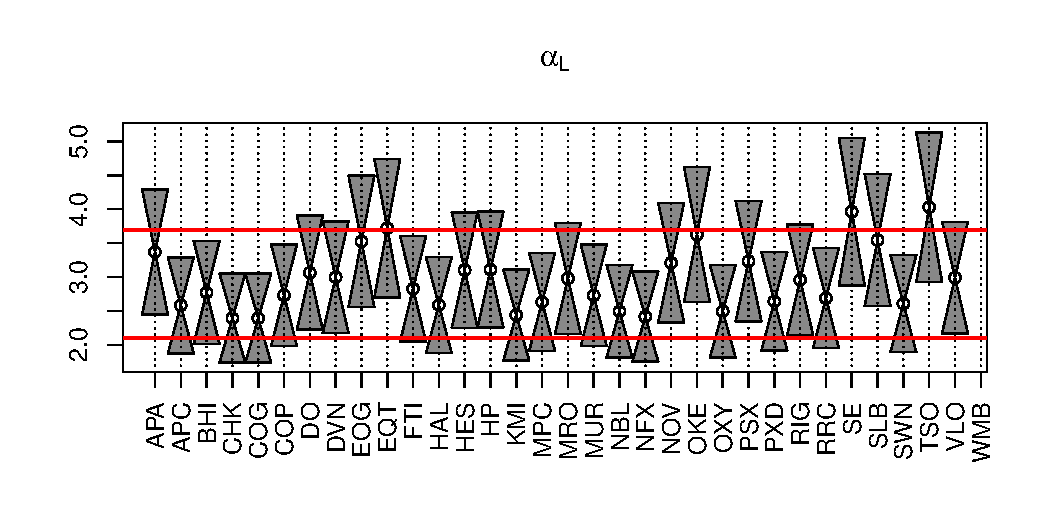
\includegraphics[width=\textwidth, trim={0, 0.8cm, 0, 2cm}, clip]
    {Energy_lower.pdf}
  \end{minipage}
  \begin{minipage}{1.0\linewidth}
    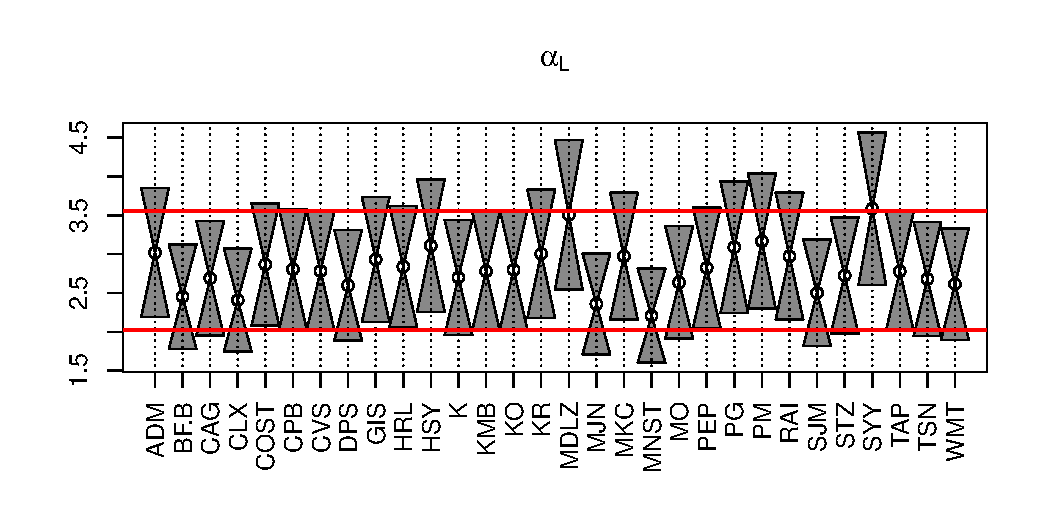
\includegraphics[width=\textwidth, trim={0, 0.8cm, 0, 2cm}, clip]
    {Consumer_Staples_lower.pdf}
  \end{minipage}
  \begin{minipage}{1.0\linewidth}
    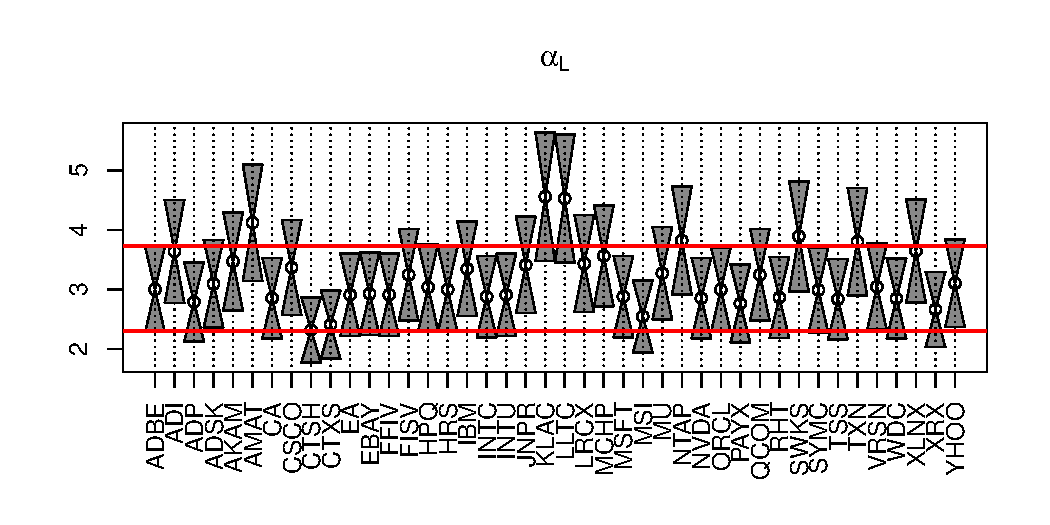
\includegraphics[width=\textwidth, trim={0, 0.8cm, 0, 2cm}, clip]
    {Information_Technology_lower.pdf}
  \end{minipage}
  \caption{\small Hill estimates $\hat \alpha_{50}$ of the lower tail-indices $\alpha$ of
    daily return series in sectors of the S\&P 500
    index. The data span
    from 1 January 2010 to 31 December 2014 and comprise $n=1304$ observations.
The graphs from top to bottom correspond to the ``Energy'',
    ``Consumer Staples'' and ``Information Technology'' sectors.
    Each circle corresponds to a Hill estimate $\hat\alpha_{50}$; the gray
    triangles above and below it mark the 97.5\% and 2.5\% quantiles
    of its approximate normal distribution; see \eqref{eq:2} and the discussion following it for an 
interpretation.
    The lower and upper red lines mark the medians of the 2.5\% 
    and 97.5\% quantiles, respectively, evaluated from all stocks in the sector.
    The data are taken from {\it Yahoo Finance}; the labels on
    the horizontal axes are Yahoo symbols of the stocks. 
  }\label{fig:1}
\end{figure}

In Figure~\ref{fig:1} we see significant overlap of the confidence intervals of the Hill
estimates of the losses in the ``Energy'' and ``Consumer Staples''
sectors of the S\&P 500 index, as well as those of a 
large portion of losses in the ``Information Technology'' sector.
This fact indicates that the returns in each sector may 
have comparable tail-indices.
\par
Hoga's \cite{hoga:2016} test about the change of extreme quantiles
in a sample
may provide some further insight about how similar these tail-indices are.
Different tail-indices are likely to result in different
extreme quantiles. Nevertheless, changes in the extreme quantiles may also
result from changing scale parameters in the tail. Therefore  we first investigate the scale
parameters of daily stock returns in the same sectors of S\&P 500 before we apply the test.


\subsection{Hill estimates of lower-tail scale parameters}\label{sec:HillScaleEstimates}
We assume the pure Pareto model \eqref{eq:3} with scale parameter $K>0$.
Hill \cite{hill1975simple} proposed  the maximum-likelihood estimator of $K$
derived from the joint \ds\ of $k$ upper order statistics in the sample; cf.
Embrechts et al. \cite{embrechts:klueppelberg:mikosch:1997}, p.~334.
It is given by
\beao
\hat K_k = \left({k \over n}\right)^{1/\hat\alpha_k} X_{(n-k)}\,.
\eeao
Using the asymptotic normality property of upper order statistics
(cf. de Haan and Ferreira~\cite{haan:ferreira:2006}, Theorem 2.2.1), one can show
\beao
  \sqrt{k}\, (\hat K_k - K) &\std& N\big(
    0, (K /\alpha)^2\big)\quad\mbox{and}\quad
  \sqrt {k} \,(\hat K_k^\alpha - K^\alpha) \overset{d}{\to} N\big(
    0, K^{2\alpha}  \big)\,,
\end{eqnarray*}
where the tail-index $\alpha$ is regarded as known. From the above
asymptotic normality property, confidence bands of $\hat K_k$
and $\hat K_k^{\hat\alpha}$ can be constructed.   
Estimates $\hat K_k$ in the ``Energy'', ``Consumer Staples'' and
``Information Technology'' sectors of the S\&P 500 index are computed
using this method. The results are shown in
Figure~\ref{fig:sectors_parameters}.
\begin{figure}[htb!]
  \centering
  \begin{minipage}{0.33\linewidth}
    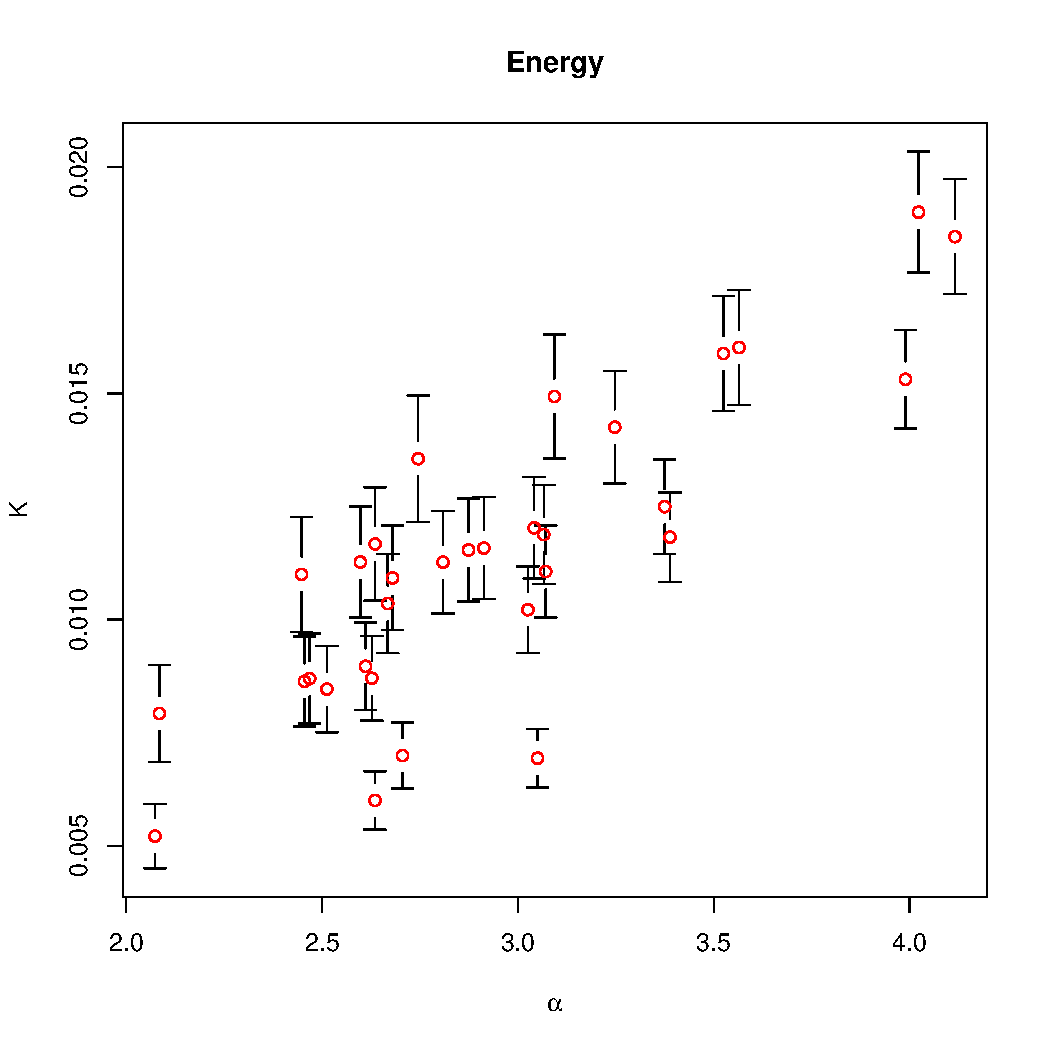
\includegraphics[width=\textwidth]
    {Energy_K.pdf}
  \end{minipage}\hfill
  \begin{minipage}{0.33\linewidth}
    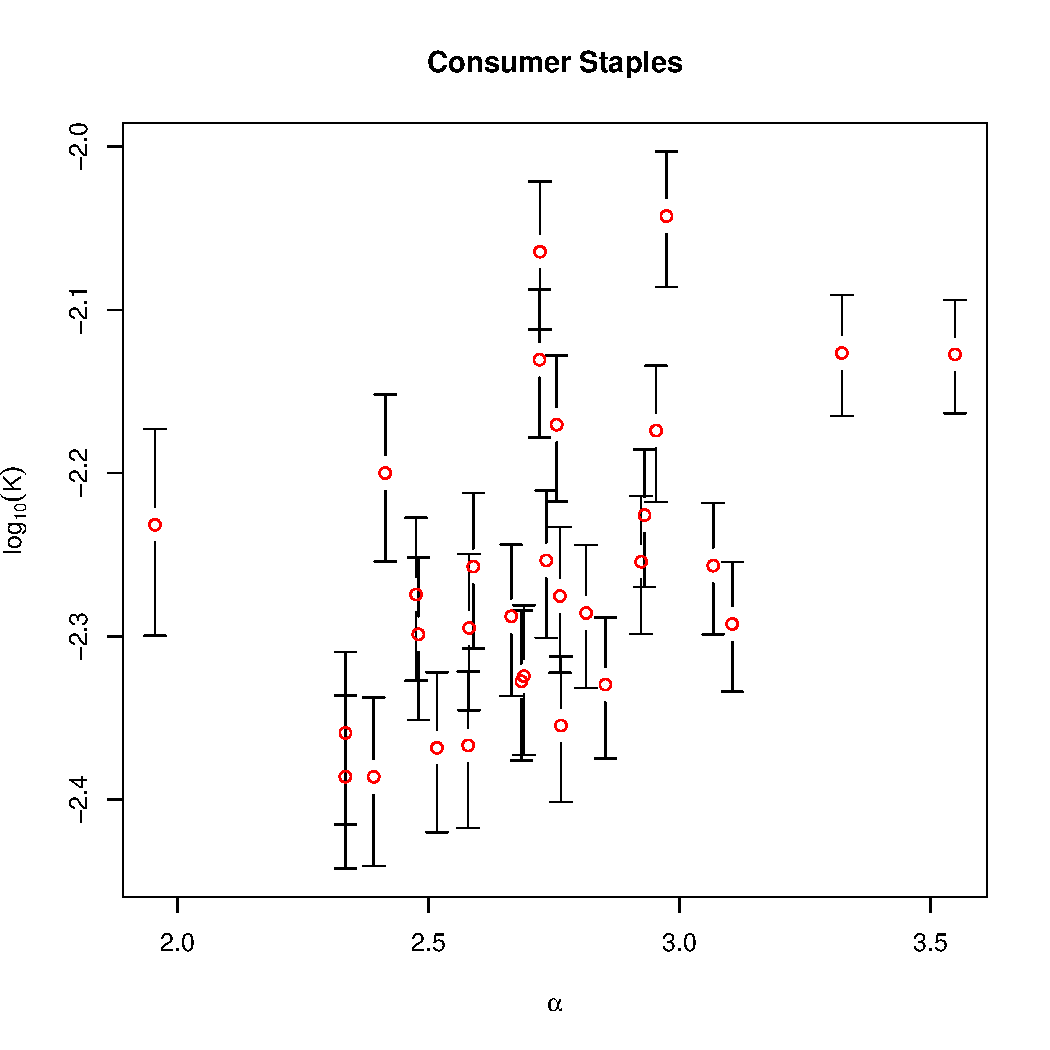
\includegraphics[width=\textwidth]
    {CS_K.pdf}
  \end{minipage}\hfill
  \begin{minipage}{0.33\linewidth}
    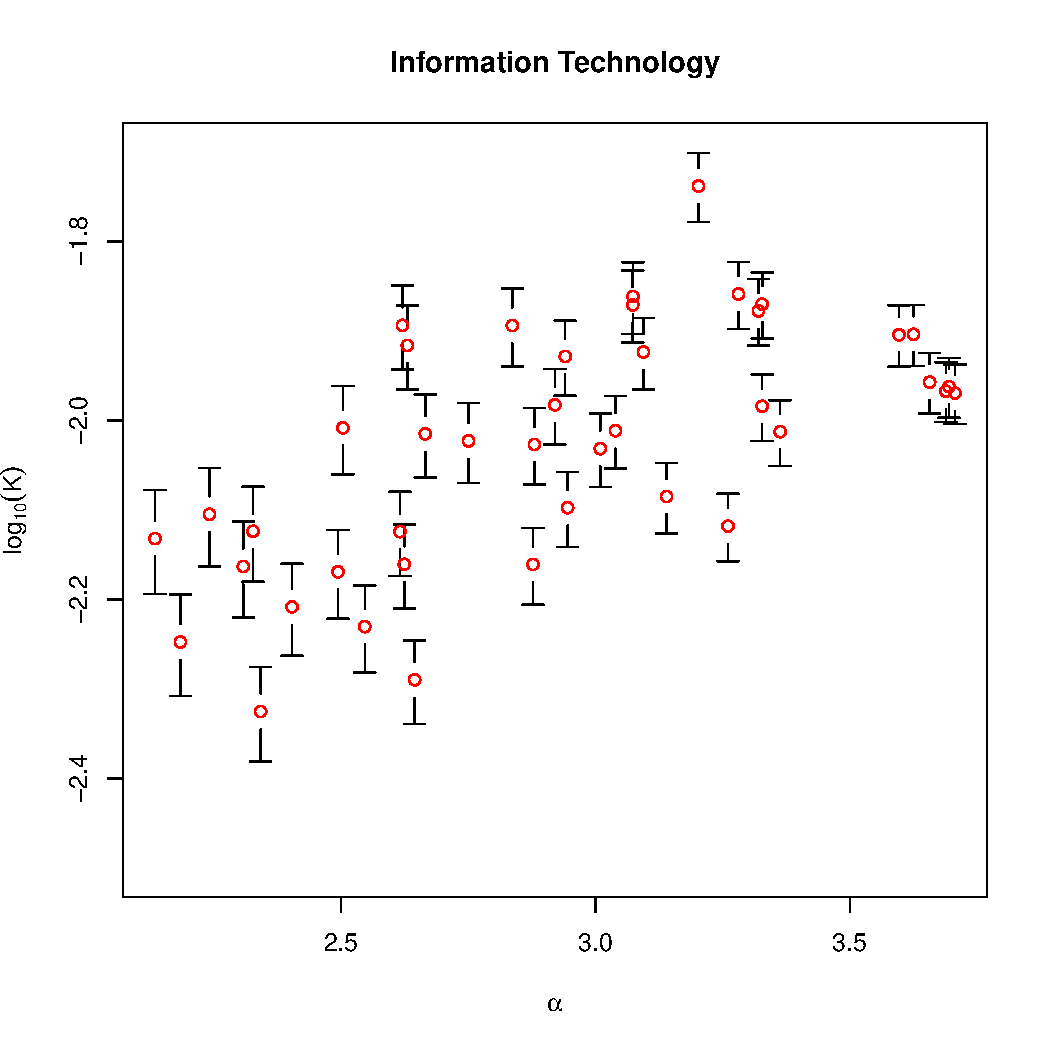
\includegraphics[width=\textwidth]
    {IT_K.pdf}
  \end{minipage}
  \begin{minipage}{0.33\linewidth}
    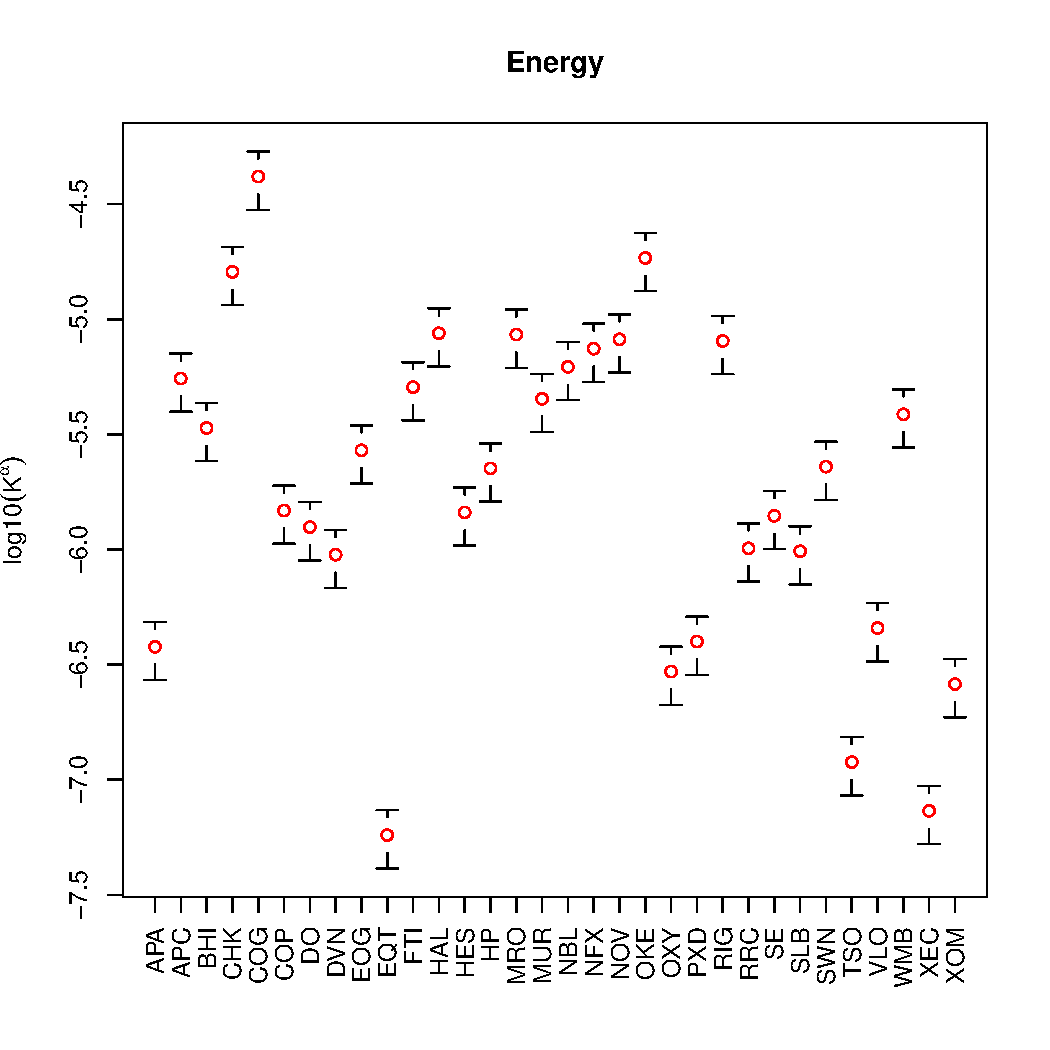
\includegraphics[width=\textwidth]
    {Energy_scale.pdf}
  \end{minipage}\hfill
  \begin{minipage}{0.33\linewidth}
    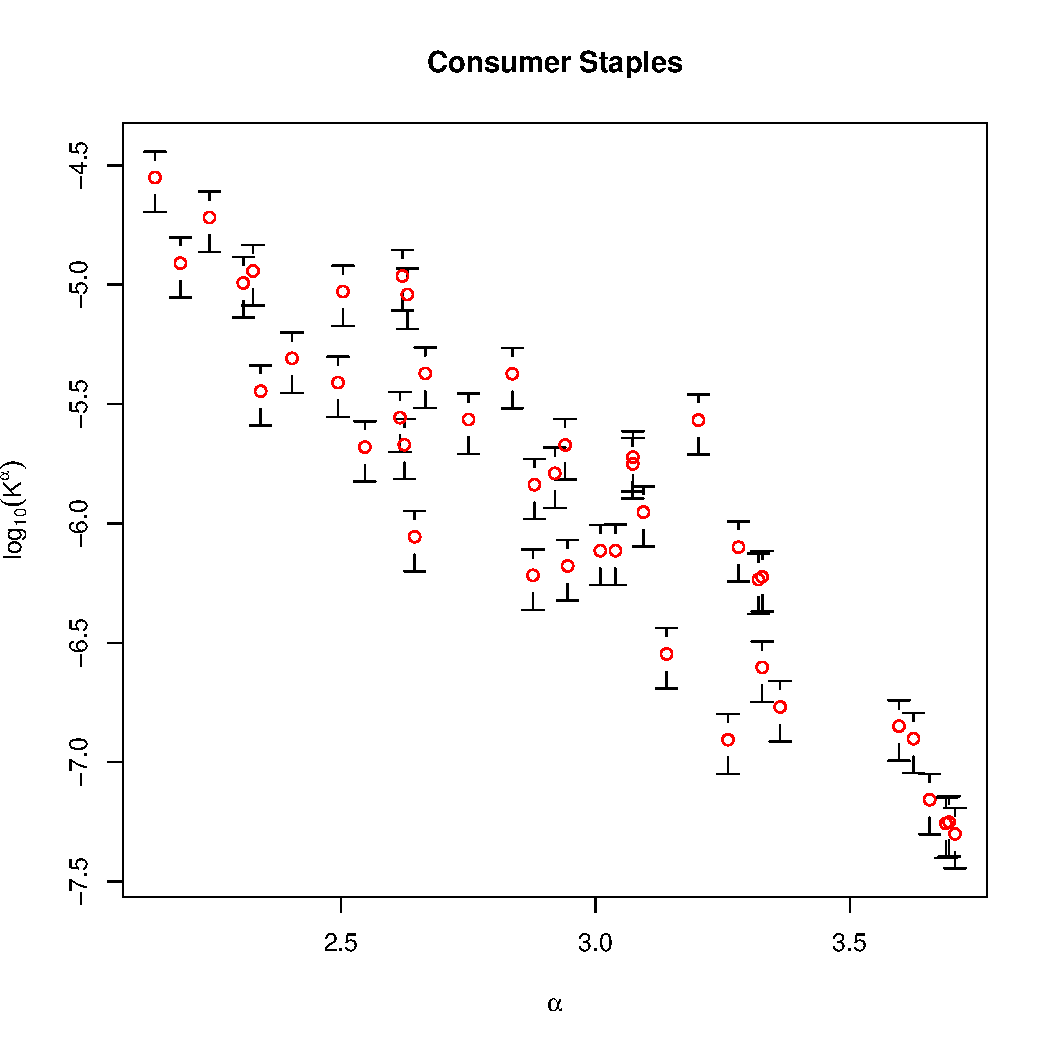
\includegraphics[width=\textwidth]
    {CS_scale.pdf}
  \end{minipage}\hfill
  \begin{minipage}{0.33\linewidth}
    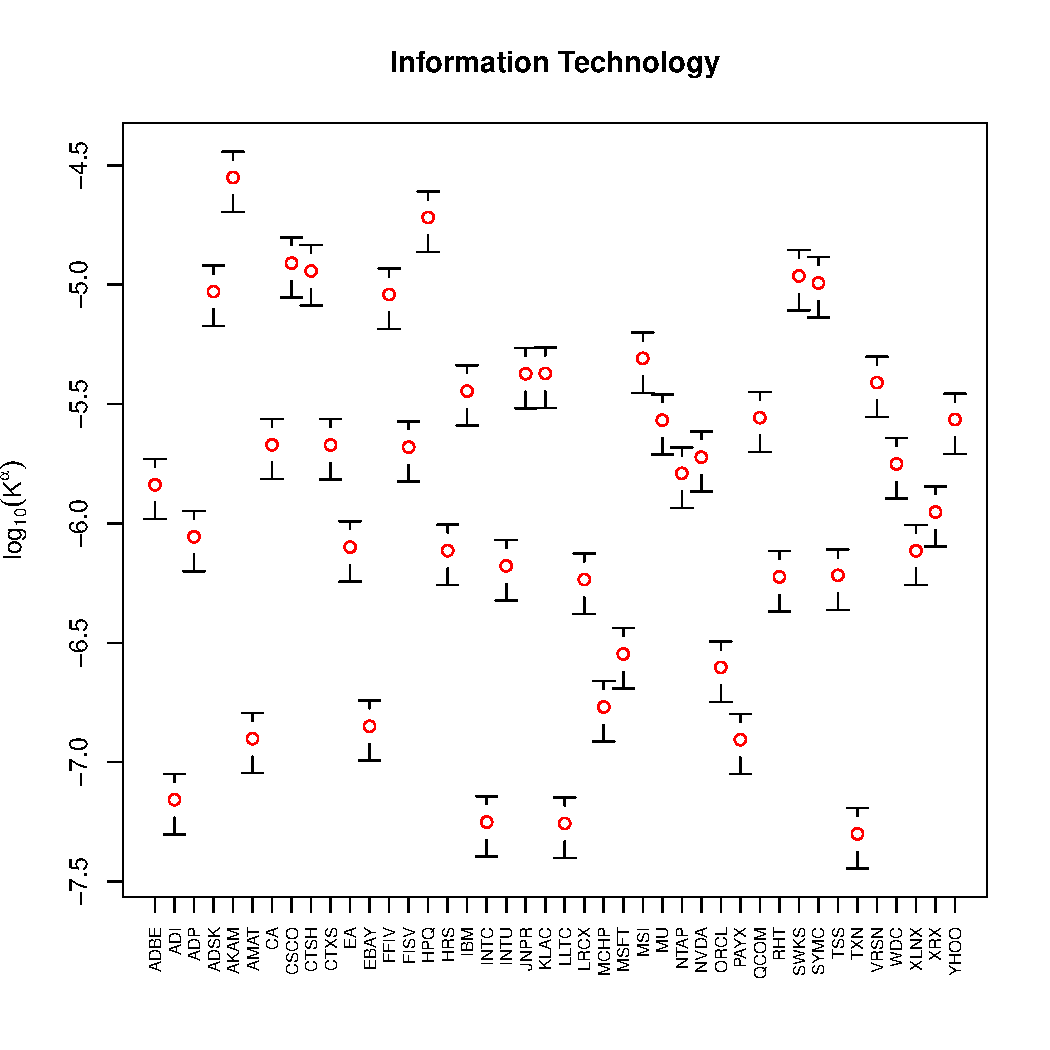
\includegraphics[width=\textwidth]
    {IT_scale.pdf}
  \end{minipage}
  \caption{\small Estimates of $\hat K_k$ (top) and $\hat K_k^{\hat
      \alpha}$ (bottom) on $\log_{10}$-scale of stocks in sectors
    of the S\&P 500 index. The estimates are ordered according to the 
    corresponding estimated $\alpha$-values.
    The points are the estimated values, the bars 
    the \asy\ 95\%-confidence intervals; the confidence bands of the
    corresponding Hill estimates $\hat \alpha_k$ of these sectors are
    shown in Figure~\ref{fig:1}. 
  }
  \label{fig:sectors_parameters}
\end{figure}
One can see that $K$ generally takes a rather small value. For the
more volatile sectors of ``Energy'' and ``Information Technology'',
the average value of $K$ is around 0.01, while for the more stable
sector of ``Consumer Staples'', the average value is around 0.005. Due
to the smallness of $K$, mild variations of $\alpha$ would lead to
huge variations of $K^\alpha$, as shown in the 2nd row of
Figure~\ref{fig:sectors_parameters}.
\par
Secondly, it appears that there is positive dependence between the
values of $\alpha$ and $K$.
As argued in Section~\ref{sec:pareto_tail}, this is consistent with
the assumption that the return series have Pareto tails on both sides
with the tail parameters on each side independent of those on the
other.

\par
Thirdly, Figure~\ref{fig:sectors_parameters} shows that, on
average, the values of $K$
in the ``Energy'' and ``Information Technology'' sectors are  larger
than those in the ``Consumer Staples'' sector.  For a given loss
probability, a larger value of $K$ implies that large losses are more
probable. Thus one can conclude that these two sectors are
considerably riskier than the ``Consumer Staples'' sector. This is of
course a confirmation of one's economic instinct.

Yet another indication from Figure \ref{fig:sectors_parameters} is
that, while the ``Energy'' and the ``Information Technology'' sectors
are similar in riskiness, the dependence  between $\alpha$ and $K$ is
stronger in ``Energy''. As discussed in Section~\ref{sec:3} below, when moving along
a curve of equal preference in the direction of increasing $\alpha$, the parameter $K$ also
increases. So the strong positive dependence seen in the ``Energy''
sector suggests that these stocks might have very similar investor
preferences. This in turn may be attributed to stronger business
relations between the energy enterprises. While two IT companies
may provide a variety of products and services and do not depend on each
other, two energy companies are more likely to depend on each other
via relations of supplier and customer or otherwise to compete with each
other if they are on the same link of the chain of energy production
and distribution.

\subsection{A test for equal tail-indices based on Hill estimation}
Suppose we have two independent strictly stationary positive series $X_1, \dots, X_n $ and
$Y_1, \dots, Y_n$ with corresponding distribution functions $F_X$ and
$F_Y$ that have power-law tails  with indices $\alpha_X$ and
$\alpha_Y$, respectively. From \eqref{eq:2} one can deduce
\begin{equation}
  \label{eq:x3}
  \sqrt k
  \begin{pmatrix}
    {\hat \alpha_X - \alpha_X} \\
    {\hat \alpha_Y - \alpha_Y} \\
  \end{pmatrix} \overset{d}{\to}
  \begin{pmatrix}
    Z_X \\
    Z_Y
  \end{pmatrix}
  \sim
  N\left(
    0, \text{diag}(\alpha_X^2, \alpha_Y^2)
  \right)
\end{equation}
where $\hat \alpha_X$ and $\hat \alpha_Y$ are Hill estimators of
$\alpha_X$ and $\alpha_Y$; we suppress their dependence on $k$. Then it follows from the continuous mapping
theorem
\begin{equation}
  \label{eq:x1}
  \sqrt k [(\hat \alpha_X -\alpha_X) - (\hat \alpha_Y - \alpha_Y)]
  \overset{d}{\to}
  Z_X - Z_Y \sim N(0, \alpha_X^2 + \alpha_Y^2)\,.
\end{equation}
This relation allows one to construct an \asy\ test under 
the null hypothesis $\alpha_X = \alpha_Y$ and with test statistic $\hat \alpha_X - \hat \alpha_Y$.
We apply this test to the equities in the ``Energy'',
``Consumer Staples'' and ``Information Technology''
sectors of the S\&P 500 index. The results are shown in the top row of
Figure~\ref{fig:PairTest}.
\begin{figure}[htb!]
  \begin{minipage}{0.33\linewidth}
    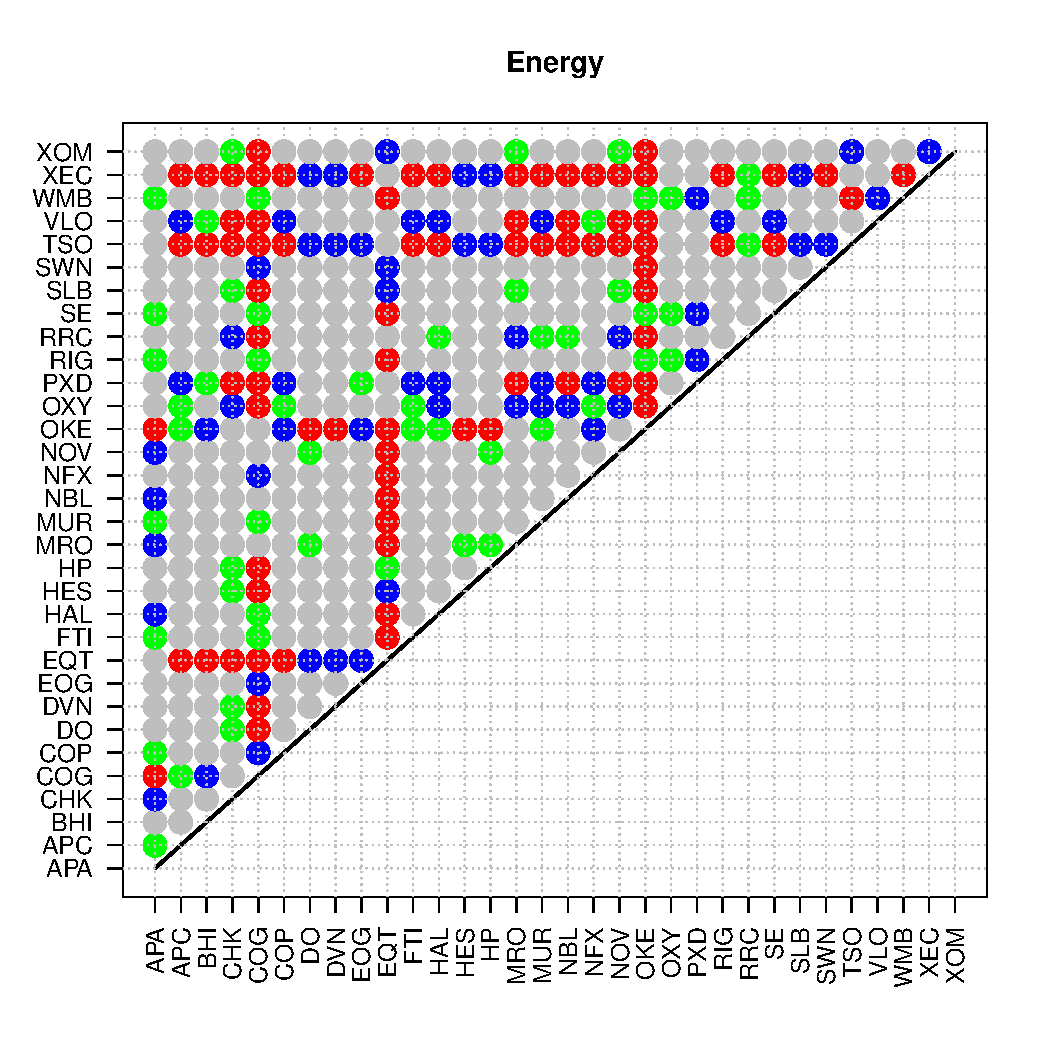
\includegraphics[
      width=\textwidth,
      trim={0.3cm, 0.8cm, 1cm, 0.6cm}, clip
    ]{HillTest_Energy.pdf}
  \end{minipage}\hfill
  \begin{minipage}{0.33\linewidth}
    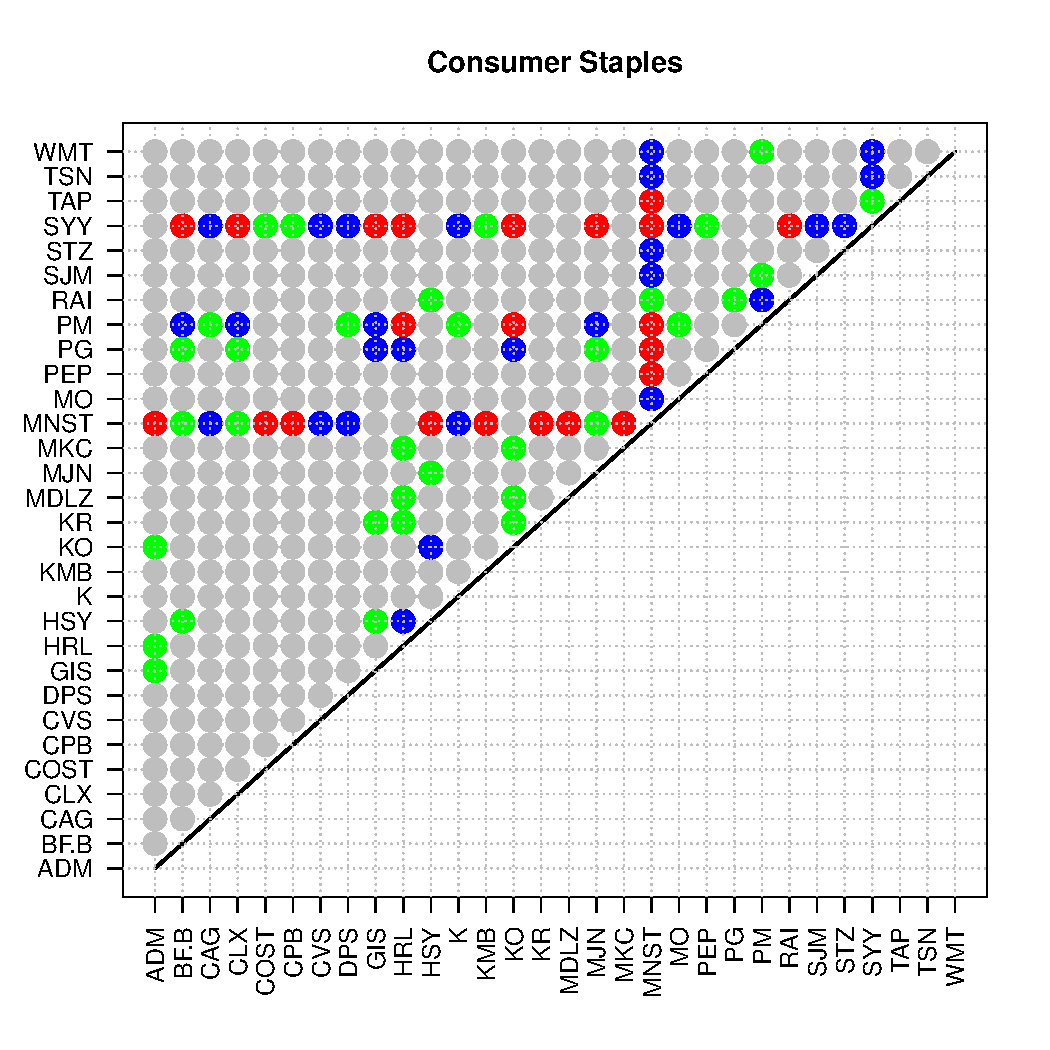
\includegraphics[
      width=\textwidth,
      trim={0.3cm, 0.8cm, 1cm, 0.6cm}, clip
    ]{HillTest_CS.pdf}
  \end{minipage}\hfill
  \begin{minipage}{0.33\linewidth}
    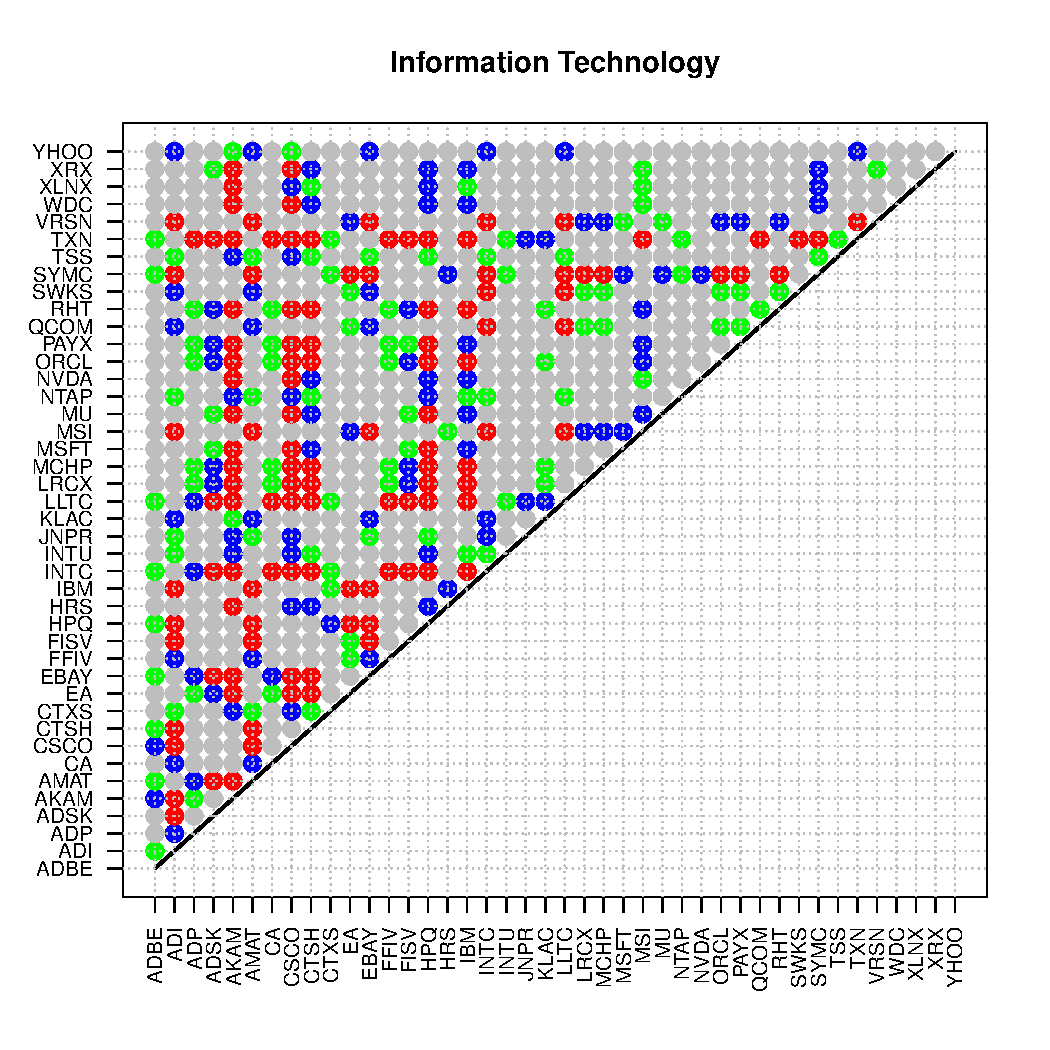
\includegraphics[
      width=\textwidth,
      trim={0.3cm, 0.8cm, 1cm, 0.6cm}, clip
    ]{HillTest_IT.pdf}
  \end{minipage}
  \begin{minipage}{0.33\linewidth}
    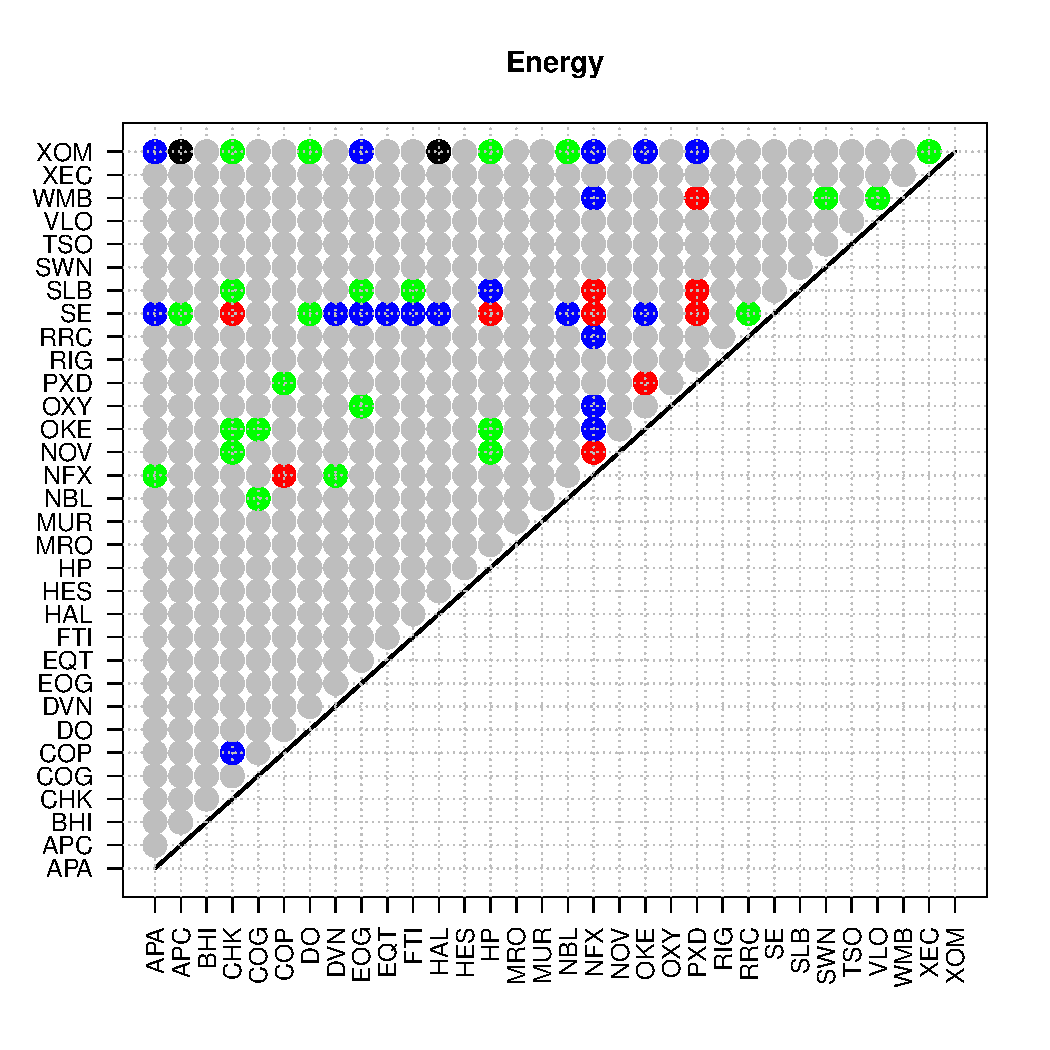
\includegraphics[
      width=\textwidth,
      trim={0.3cm, 0.8cm, 1cm, 0.6cm}, clip
    ]{Hoga_Energy_pair.pdf}
  \end{minipage}\hfill
  \begin{minipage}{0.33\linewidth}
    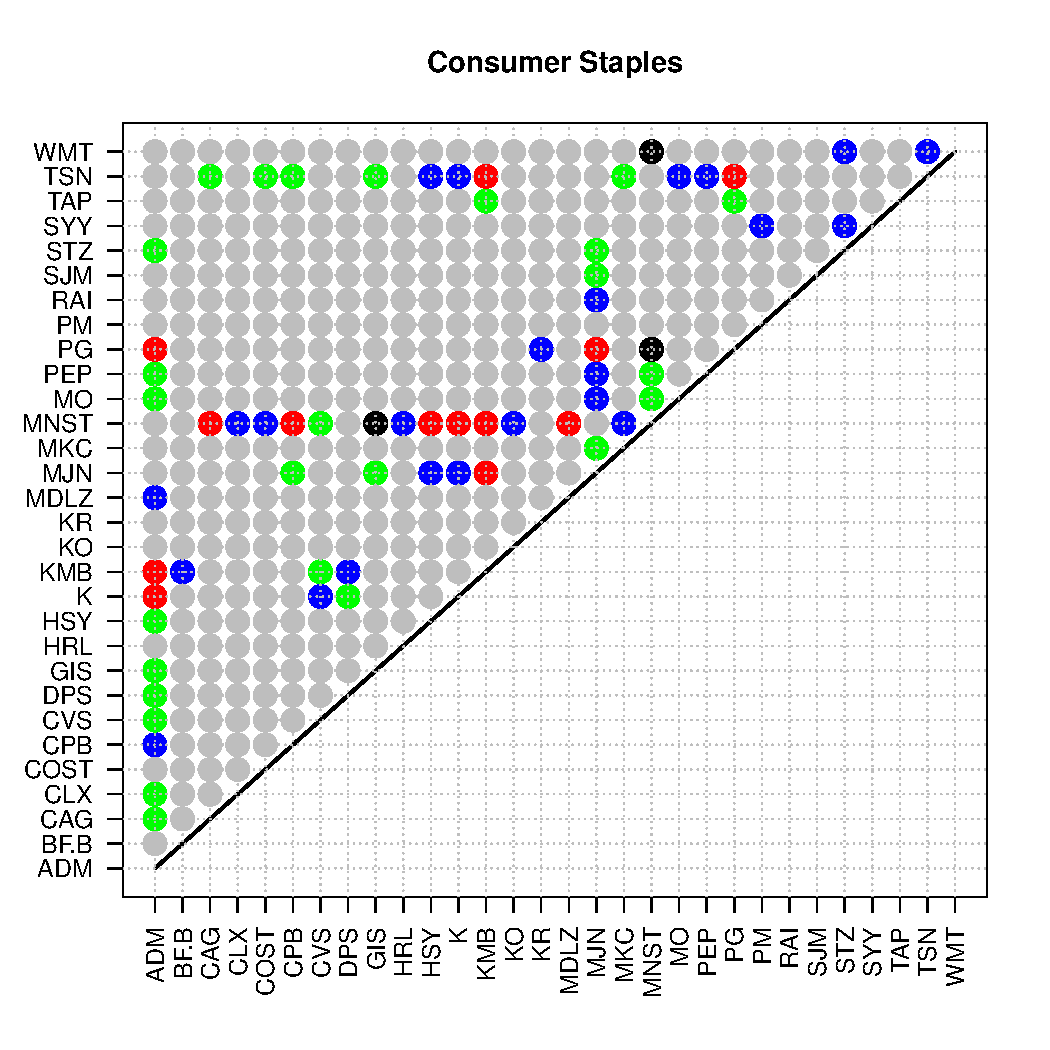
\includegraphics[
      width=\textwidth,
      trim={0.3cm, 0.8cm, 1cm, 0.6cm}, clip
    ]{Hoga_CS_pair.pdf}
  \end{minipage}\hfill
  \begin{minipage}{0.33\linewidth}
    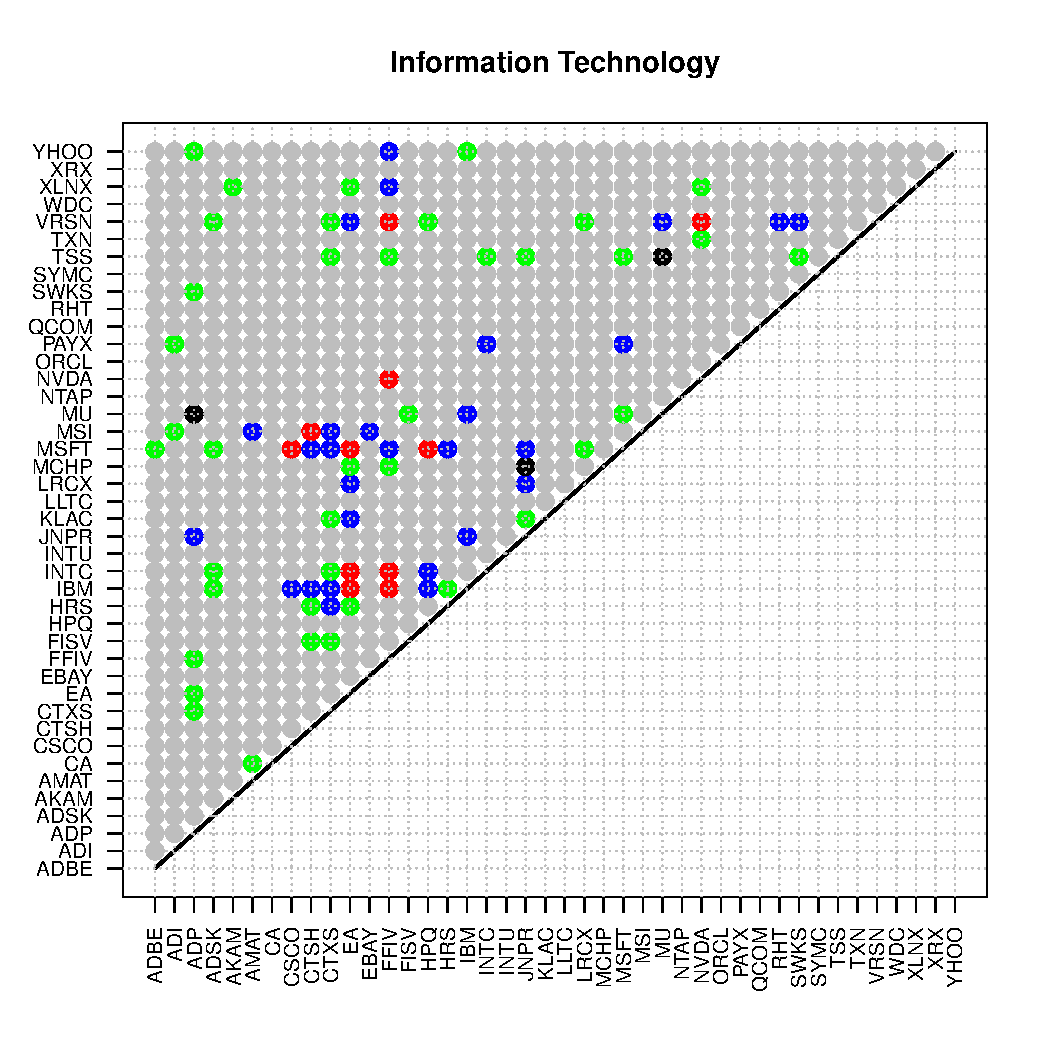
\includegraphics[
      width=\textwidth,
      trim={0.3cm, 0.8cm, 1cm, 0.6cm}, clip
    ]{Hoga_IT_pair.pdf}
  \end{minipage}
  \caption{{\em Top row}: Test for pairwise equality of tail-indices
    of losses in the  ``Energy'', ``Consumer Staples'' and
    ``Information Technology'' 
    sectors of S\&P 500. The test statistic in $\hat\alpha_X-\hat \alpha_Y$ is based
    on Hill estimates 
    of $\alpha_X$ and $\alpha_Y$. 
    The green, blue and red points correspond to pairs of stock in a sector
    when the test statistic is outside the intervals $[q_{0.075},q_{0.925}]$,
    $[q_{0.05},q_{0.95}]$,  $[q_{0.025},q_{0.975}]$, respectively, where
    $q_p$ is the $p$-quantile of the limiting 
    $N(0,\alpha_X^2+\alpha_Y^2)$-\ds\ of the test statistic in
    \eqref{eq:x1}. Grey points stand for pairs for which the test
    statistic is inside $[q_{0.075},q_{0.925}]$. 
    {\em Bottom row:} Test for changing tail-index or scale parameter
    of losses
    using Hoga's test based on concatenated series of pairs of
    stocks. The green, blue and red points
    correspond to pairs of stock in a sector 
    when the test statistic $T_n$ exceeds the $85\%$-, $90\%$-,
    $95\%$-quantile of the limit \ds .
  Grey points stand for pairs for which the test statistic is below
  the \asy\ $85\%$-quantile. Black points represent 
    pairs for which the computation of $T_n$ fails for given precision  
    requirements and time limits.
    The same number (50) of upper order statistics is used for both tests.}
  \label{fig:PairTest} 
\end{figure}
They indicate that tail-indices of equities in the
``Energy'' or ``Information Technology'' sectors are more variable 
than in the ``Consumer Staples'' sector, as the null
hypothesis is rejected more often for members of these two former sectors.
Moreover, these figures suggest that the test based on the Hill estimator
is quite powerful in distinguishing between tail-indices. In contrast to the test presented in Section~\ref{sec:Hoga}
the present test results in  more rejections for the ``Energy'' and the
``Information Technology'' sectors.
\par
As a caution, one should bear in mind that 
\eqref{eq:x3} is valid on condition that the $X$- and $Y$-
series are independent of each other (or weakly dependent on each other), which is generally untrue for
two return series in the same market.

\subsection{A test for a change in the extreme tail}\label{sec:Hoga}
Here we apply a test from
a recent paper by Hoga \cite{hoga:2016}. This test has been developed
for a different kind of problem. Given a strictly stationary
\ts\ $X_1,\ldots,X_n$ with a marginal \ds\ $F$ with right power-law
tail, the goal is to test whether there is a structural break of the
{\em extreme quantiles} $F^{-1}(1-p)$ for values $p$ very close to
zero. If the tail-index {\em or} the scale parameter in a \ds\ of type
\eqref{eq:3} change inside a sample, then it is likely that the
extreme quantiles change as well. We will test for a change of tail-index or scale parameter in this indirect way.
\par
The null hypothesis of the test in \cite{hoga:2016} is that there is no change of the extreme quantiles $F^{-1}(1-p)$ 
for $p=p_n\to 0$ in any subsample with indices
$t\in (n\,t_0,n(1-t_0))$ where $t_0$ is a fixed number in $(0,0.5)$. Writing $\hat x_p(a,b)$ for an estimator of the extreme $(1-p)$-quantile 
based on the subsample with indices $t\in (na,nb)$, the test statistic
is given by
\begin{small}
  \beam\label{eq:4}
  T_n = \sup_{s \in [t_0, 1 - t_0]}
  \dfrac{  \big[s (1 - s) \log \big(\hat x_p(0, s)/\hat x_p(s, 1)\big)
      \big]^2}{
    \int_{t_0}^s\big[r \log \big( \hat x_p(0, r)/\hat x_p(0, s)
      \big)
      \big]^2 dr
    +
    \int_{s}^{1 - t_0}
    \big[
      (1 - r) \log \big(
      \hat x_p(r, 1)/
      \hat x_p(s, 1)
      \big)
      \big]^2 dr}\nonumber\\
  \eeam
\end{small}
Under the null hypothesis, $(T_n)$ converges to a complicated \fct al
of Brownian motion\ on $[0,1]$; the \asy\ quantiles need to be
evaluated by simulation.
\par
When applied to our problem we would like to test 
whether there is a change of the tail-index {\em or} scale parameter in \eqref{eq:3} in each of the S\&P 500 
series in the distinct sectors. We also  want to get some indication about a possible change of tail-index or
scale parameter from one series to another within a given sector. For this reason, we choose any pair of series
within a sector and concatenate each of the paired series. Then we run the test on the concatenated series.
Of course, despite the fact that we test changes of tail-index or scale parameter 
{\em in a very indirect way} -- there may be many other reasons for the change of extreme quantiles in a sample -- 
we also concatenate two rather distinct series. Even if we assume that the two series come from related models
(such as GARCH), the parameters of these models will in general not be the same. Moreover, the concatenation
of two strictly stationary \ts\ is in general not strictly stationary. Therefore we have to be careful
with interpretations of the results of the tests.
\par 
In Figure~\ref{fig:Hoga_Single} we show the values of the test statistic $T_n$ (horizontal bars)
for $t_0=0.1$ and daily return series of stock in the ``Energy'' and ``Consumer Staples'' sectors of the S\&P
500 index. The ``null hypothesis'' is that the tail-index and scale parameter remain the
same throughout the selected period of time. For most stocks, the hypothesis cannot be rejected even at the 85\% level.
This fact may be an indication that the \ds\ inside a series is rather homogeneous.
Alternatively, it may show that the power of the test is very low. A possible reason for this suspicion is that the \con\ rate
of $(T_n)$ to its limit is very slow, i.e., the \asy\ \ds\ is not representative for the \ds\ of $T_n$ for the chosen $n$; for some
simulation evidence, see below.
\par
To check whether any pair of stocks shares the same tail-index and scale parameter we concatenate
any two series and apply the aforementioned test on the concatenated series. For the ``Energy'' and the
``Consumer Staples'' sector we summarize the results in the bottom row of Figure~\ref{fig:PairTest}.
These graphs show that the ``null
hypothesis'' of an equal tail-index and scale parameter is rejected for more pairs in the
``Energy'' sector than it is for those in the ``Consumer Staples''
sector. This suggests that lower tail-indices of stocks in the
``Energy'' sector are more spread out than those of the ``Consumer
Staples'' sector. Also observe that while 3 stocks, say A, B and C, test in favor of
the relations $\alpha_A = \alpha_B, \alpha_A \neq \alpha_C$, it often
happens that another test on B and C is supportive of $\alpha_B = \alpha_C$. Again,
this is due to the limited power of the test. Based
on such results, one may guess that $\alpha_B$ lies between $\alpha_A$ and
$\alpha_C$. The test is unable to recognize the smaller differences
between $\alpha_A, \alpha_B$ on one hand and between $\alpha_B, \alpha_C$ on the other hand.
\begin{figure}[htb!]
  \begin{minipage}{0.5\linewidth}
    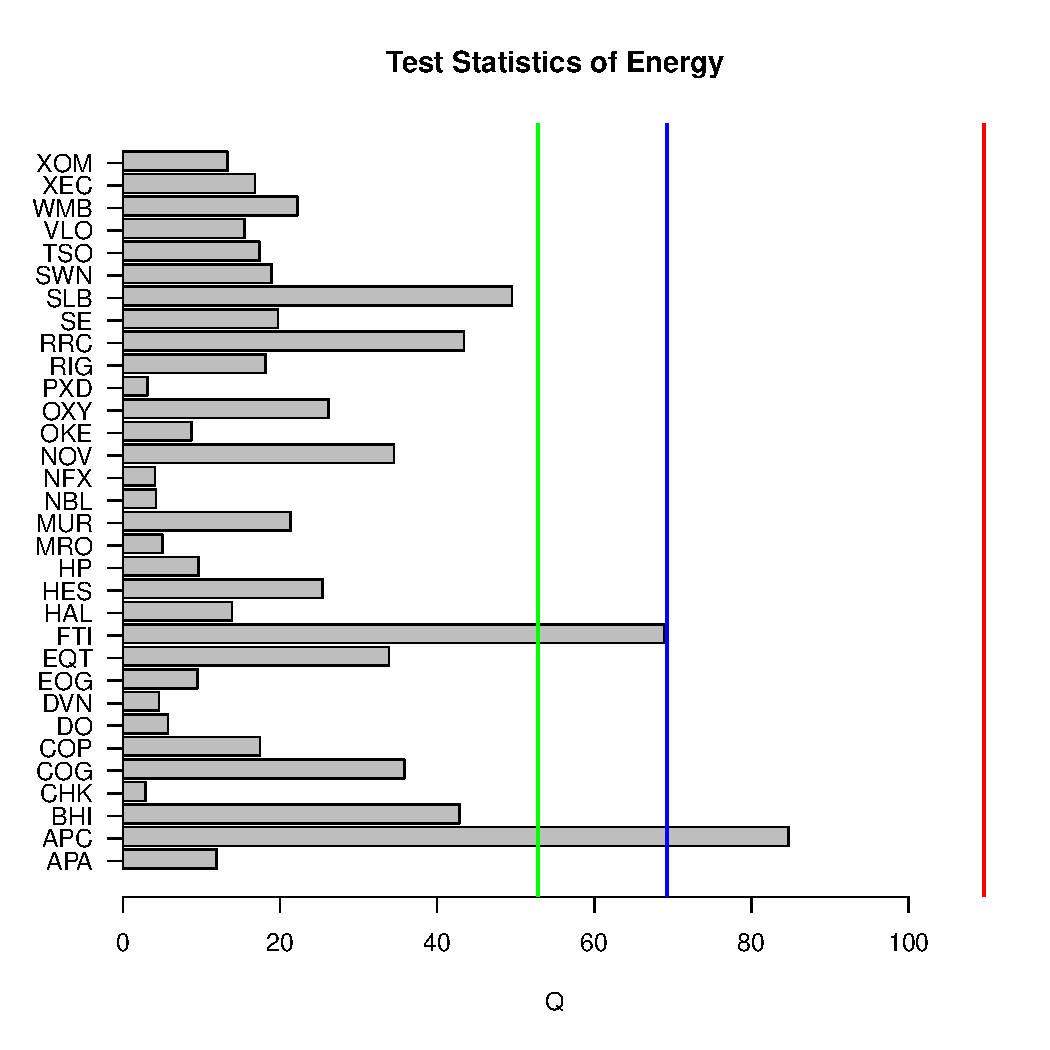
\includegraphics[width=\textwidth]
    {Hoga_Energy_Single.pdf}
  \end{minipage}\hfill
  \begin{minipage}{0.5\linewidth}
    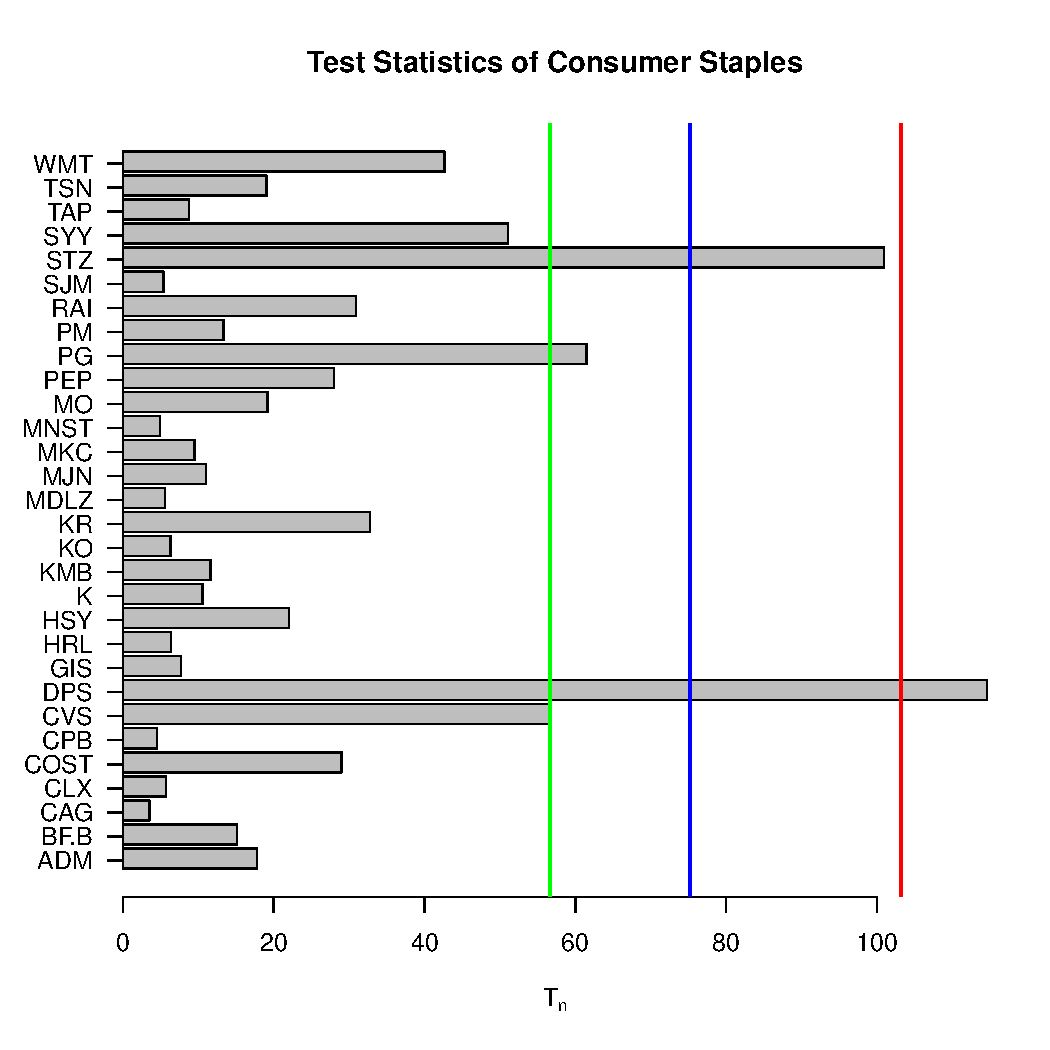
\includegraphics[width=\textwidth]
    {Hoga_CS_Single.pdf}
  \end{minipage}
  \caption{Test statistic $T_n$ from \eqref{eq:4} for the  stocks in the ``Energy'' and
    ``Consumer Staples'' sectors of S\&P 500. The green, blue and red
    lines correspond to the 85\%, 90\% and 95\% quantiles of the limit \ds\ of $T_n$.  They are derived
by simulations from the limit \ds .}
  \label{fig:Hoga_Single}
\end{figure}

To get an idea about the power of the test we run it on a
sample concatenated from two independent iid samples of the same size
$n=1304$ as the S\&P 500 series. Both pieces are $t$-distributed with
distinct degrees of freedom. The results are shown in
Figure~\ref{fig:t_sim_pair}: the power of the test is the smaller the
larger the minimum tail-index in the concatenated pair.
\begin{figure}[htb!]
  \begin{minipage}{0.5\linewidth}
    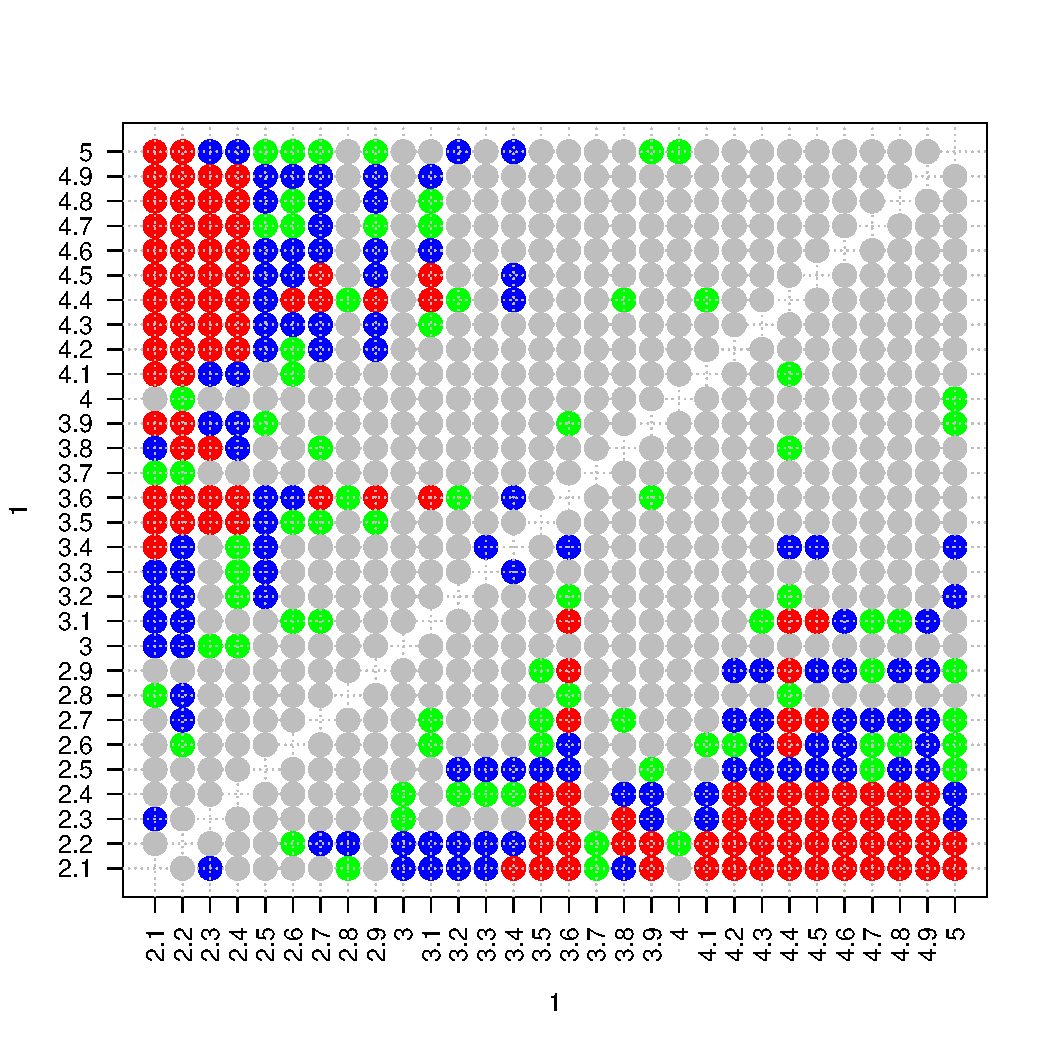
\includegraphics[width=\textwidth]{t_sim_pair.pdf}
  \end{minipage}\hfill
  \begin{minipage}{0.5\linewidth}
    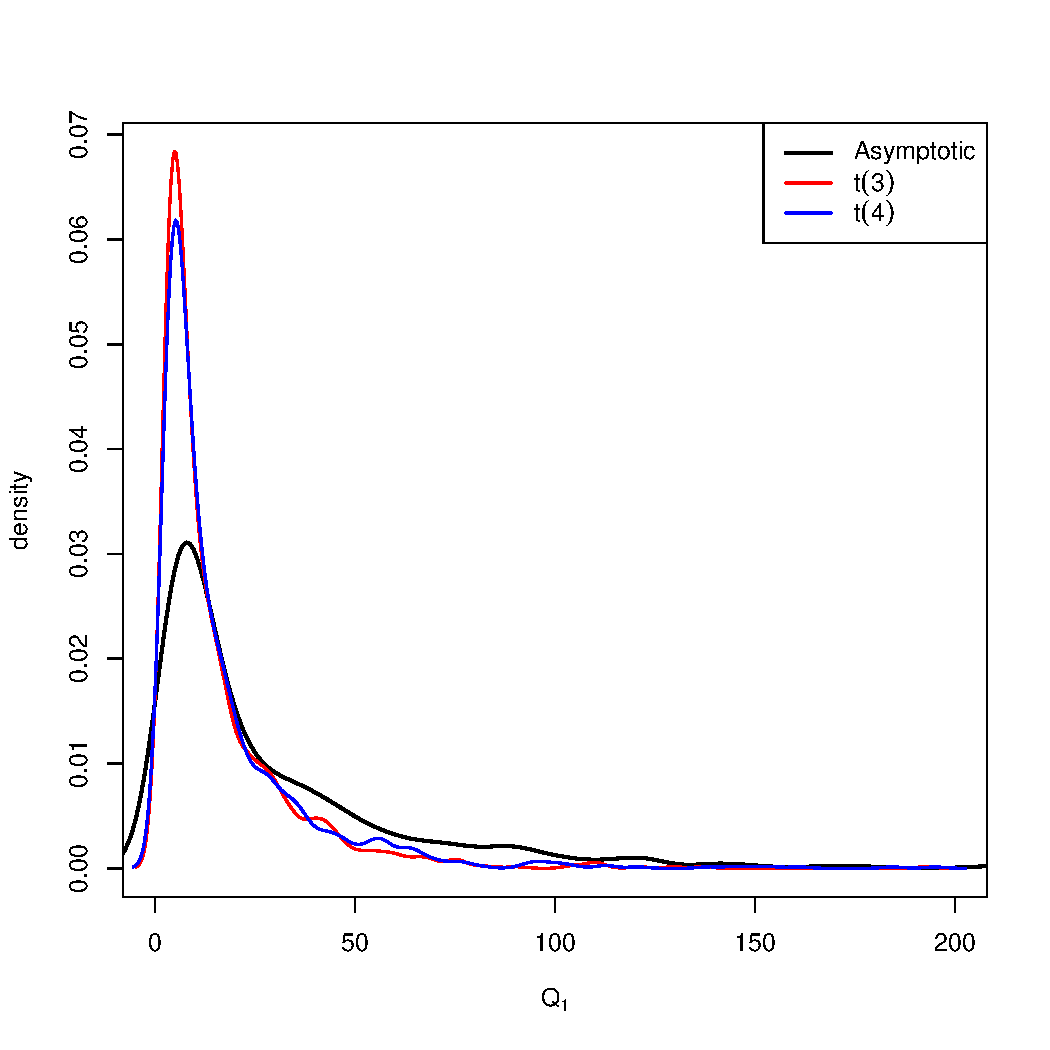
\includegraphics[width=\textwidth]{Hoga_AsymptoticDistribution.pdf}
  \end{minipage}
  \caption{
    {\em Left}: Test  of concatenated $t$-samples with different
    degrees of freedom $\alpha$. Numbers on the axes are the degrees of freedom
    in the subsamples. For an interpretation of the colored bullets,
    see the caption for the bottom row of Figure~\ref{fig:PairTest}. The graph shows the limited power
    of the test. In particular, if both degrees of freedom are
    relatively large it loses the capability of distinguishing between the \ds s.
    {\em Right}: Comparison of the \asy\ distribution of the test statistic
    $T_n$ in \eqref{eq:4} under the null hypothesis and the \ds\ of
    $T_n$ for $n=1304$ iid $t$-distributed $X_t$ with 3 and 4 degrees
    of freedom.
  }
  \label{fig:t_sim_pair}
\end{figure}

A major problem of this test is the \asy\ distribution of the test statistic under the
null hypothesis.  The rate at which the finite-sample distribution tends to its limit is not known.
To find out about this problem we compared the \ds s of $T_{1304}$ 
for $t$-distributed $X_t$ with  $\alpha=3$ and $\alpha=4$ degrees of freedom with
the limit \ds\ of $T_n$.
The estimated density functions are shown on the right of Figure~\ref{fig:t_sim_pair}.
As seen in the graph, the asymptotic distribution assigns
significantly more mass to the tail than the \ds s of $T_n$ do. For
comparison, we list a few quantiles of these \ds s in
Table~\ref{tab:HogaAsymptotic}, showing major differences between the
\asy\ and finite-sample \ds s.
\begin{table}[htb!]
  \centering
  \begin{tabular}{l|c|c|c|r}
    & \multicolumn{4}{c}{Quantiles} \\[2mm]
    \hline
    Distribution of $X_t$& 80\% & 85\% & 90\% & 95\% \\
    \hline
    Asymptotic & 47.48 & 59.61 & 78.90 & 113.12 \\
    t(3)  & 23.30 & 28.27 & 35.04 & 46.75 \\
    t(4)  & 25.76 & 31.13 & 38.81 & 56.32\\[2mm]
  \end{tabular}
  \caption{Quantiles of the test statistic $T_n$ for $n=1304$
    $t$-distributed samples with $\alpha=3$ and $\alpha=4$ 
degrees of freedom
    as well as the corresponding quantiles for the limiting \ds\ of
    $T_n$. In particular, there are huge differences between the three
    \ds s  for the higher quantiles. 
    }
  \label{tab:HogaAsymptotic}
\end{table}

Figure~\ref{fig:PairTest:permuted} points at another shortcoming
of the test: we show $T_n$ for an 
arbitrarily chosen random permutation of the concatenated data from two 
different stocks. In this case the null hypothesis that two series
have the same tail-index is rejected much more often, as a comparison
with the bottom graphs of
Figure~\ref{fig:PairTest} shows. If the data in the concatenated 
series were iid a random permutation would not change the 
\ds\ of $T_n$. Thus the value of the test statistic $T_n$  
strongly depends on the dependence structure of the underlying data
and therefore a test based on $T_n$ may be misleading.

\begin{figure}[htb!]
  \begin{minipage}{0.33\linewidth}
    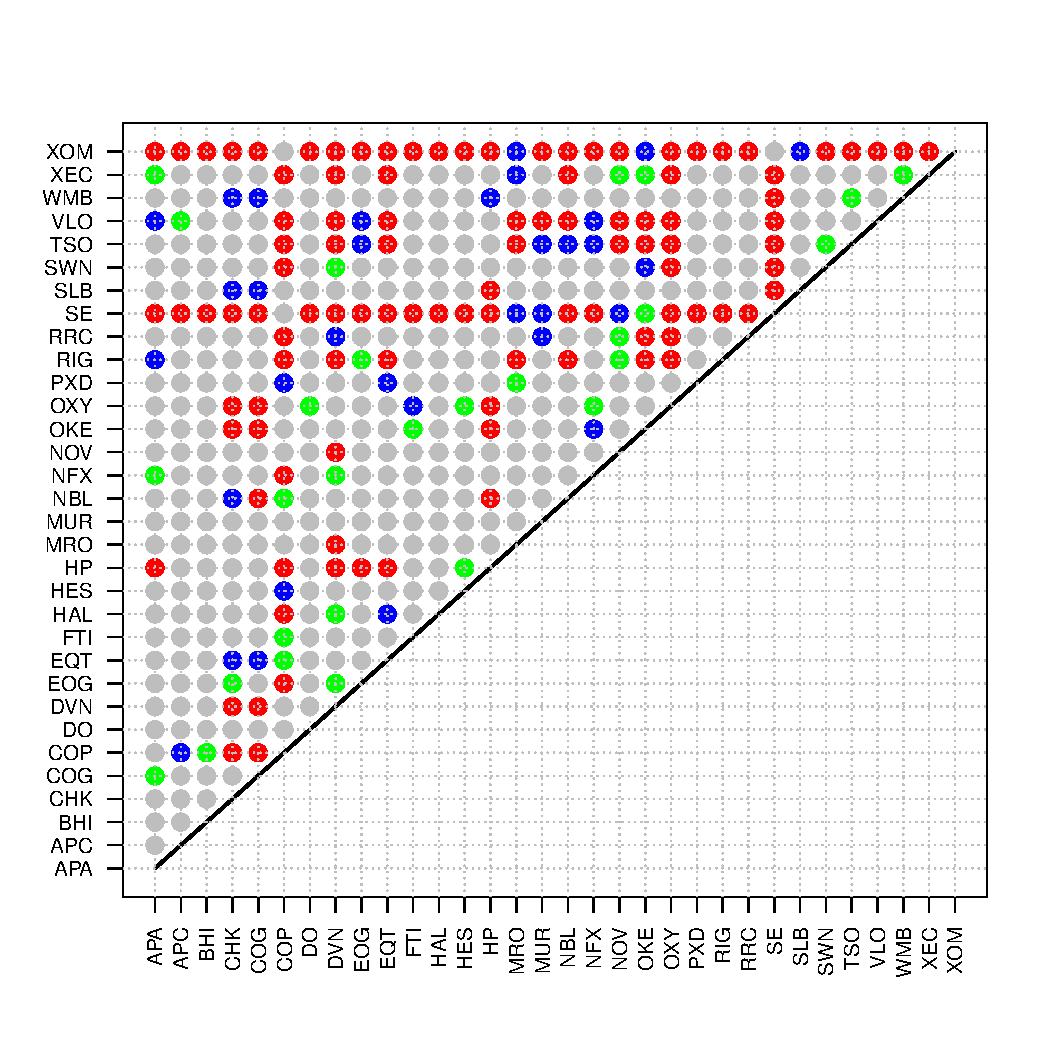
\includegraphics[
      width=\textwidth,
      trim={0.3cm, 0.8cm, 1cm, 0.6cm}, clip
    ]{Hoga_Energy_pair_permuted.pdf}
  \end{minipage}\hfill
  \begin{minipage}{0.33\linewidth}
    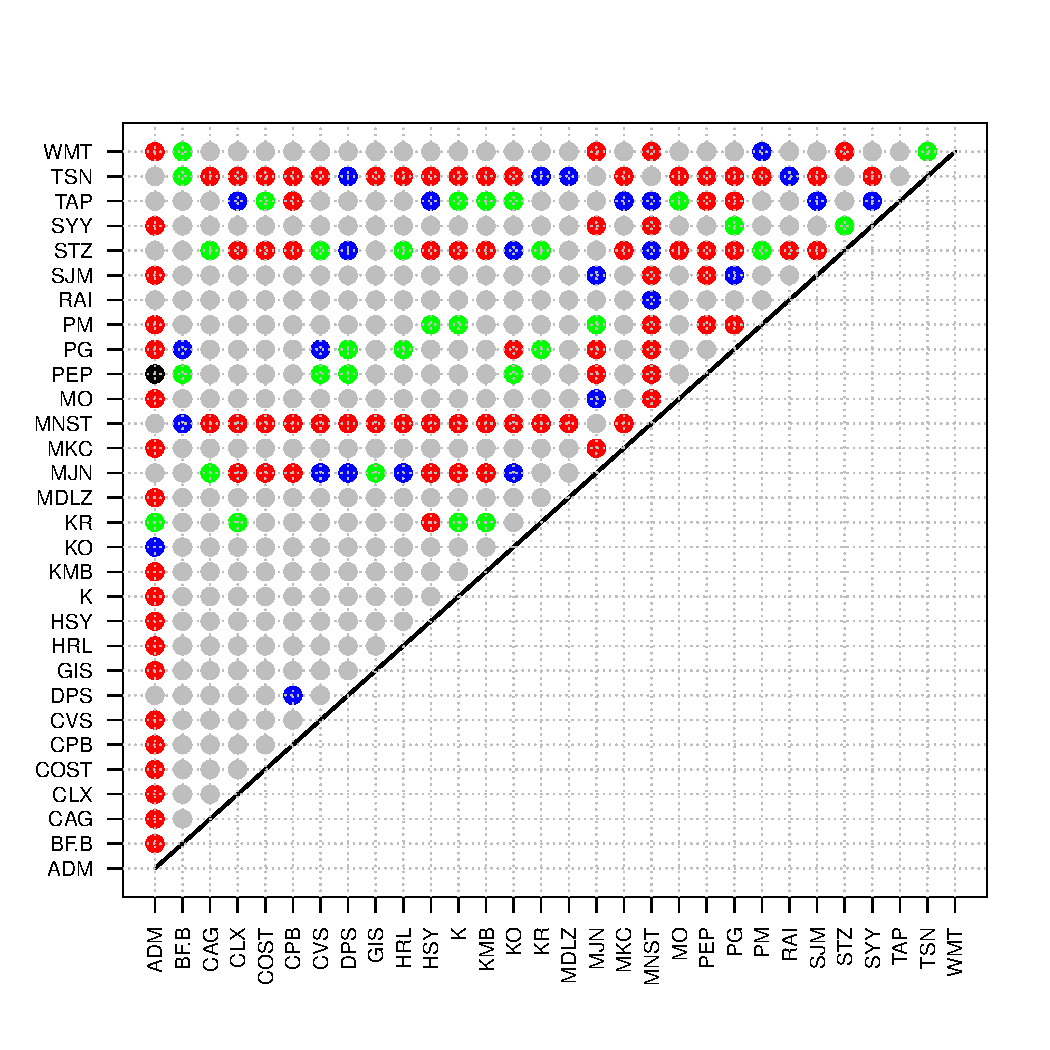
\includegraphics[
      width=\textwidth,
      trim={0.3cm, 0.8cm, 1cm, 0.6cm}, clip
    ]{Hoga_CS_pair_permuted.pdf}
  \end{minipage}\hfill
  \begin{minipage}{0.33\linewidth}
    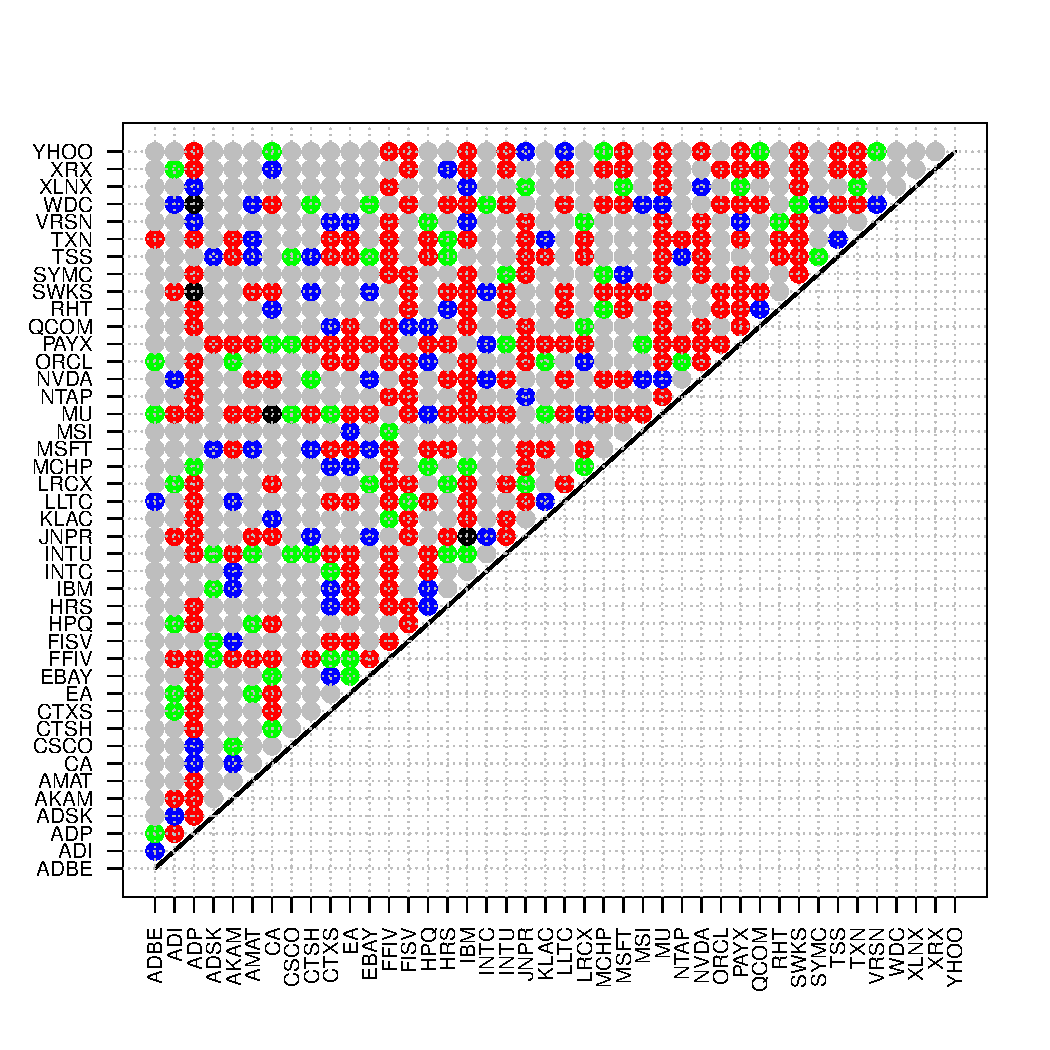
\includegraphics[
      width=\textwidth,
      trim={0.3cm, 0.8cm, 1cm, 0.6cm}, clip
    ]{Hoga_IT_pair_permuted.pdf}
  \end{minipage}
  \caption{
    Test for changing tail-index or scale parameter
    of losses
    using Hoga's test based on concatenated series of pairs of
    stocks.
    A random permutation is applied to the observations of each
    series.
    The green, blue and red points
    correspond to pairs of stock in a sector 
    when the test statistic $T_n$ exceeds the $85\%$-, $90\%$-,
    $95\%$-quantile of the limit \ds .
    Grey points stand for pairs for which the test statistic is below
    the \asy\ $85\%$-quantile. Black points represent 
    pairs for which the computation of $T_n$ fails for given precision  
    requirements and time limits.
  }
  \label{fig:PairTest:permuted} 
\end{figure}


\newpage
\section{Some theoretical arguments for equality of tail-indices}\setcounter{equation}{0}\label{sec:2}
\subsection{Multivariate GARCH models whose components have  equal tail-indices}\label{subsec:garch}
Among the models for returns the generalized autoregressive conditionally heteroscedastic (GARCH) model
is certainly most popular because it is parsimonious, captures various of the stylized facts of real return data
and can also be modified in various directions to capture specific behavior of \ts\ such a asymmetry, skewness, long memory; 
see for example Andersen et al. \cite{andersen:davis:kreiss:mikosch:2009}, Part 1, for a collection of results
on GARCH-type models.
The original  {\em univariate} GARCH model of Bollerslev \cite{bollerslev:1986} is a stochastic volatility model of the type $X_t=\sigma_t\,Z_t$, where 
$(Z_t)$ is an iid mean-zero unit-variance \seq . In the simple case of a GARCH the {\em squared volatility} satisfies the {\em stochastic recurrence equation} 
\beam\label{eq:5}
\sigma_t^2= \alpha_0+\alpha_1 X_{t-1}^2+\beta_1\sigma_{t-1}^2=\alpha_0+(\alpha_1Z_{t-1}^2+\beta_1)\sigma_{t-1}^2\,,\quad t\in\bbz\,.
\eeam
Here $\alpha_0>0$, $\alpha_1,\beta_1$ are non-negative constants. For suitable choices of $\alpha_1,\beta_1$ the equation \eqref{eq:5}
can be solved and the solution $(\sigma_t^2)$ constitutes a strictly stationary \seq , implying that $(X_t)$ 
is strictly stationary itself. A remarkable property of the process $(\sigma_t)$ is that it has a power-law tail 
of the form
\beam\label{eq:6}
\P(\sigma_t>x)\sim c\,x^{-\alpha}\,,\qquad \xto\,,
\eeam
for some positive $c>0$ and a positive tail-index $\alpha$ which is the unique solution of the equation 
$\E [(\alpha_1 Z_1^2+\beta_1)^{\alpha/2}]=1$
provided that the solution exists and some mild assumptions on the \ds\ of $Z_t$ hold. This result
follows by an application of the Kesten-Goldie theorem; see Kesten \cite{kesten:1973}, Goldie \cite{goldie:1991}, cf. 
Buraczewski et al. \cite{buraczewski:damek:mikosch:2016} for a 
recent textbook treatment. The latter result ensures power-law tails  for
the strictly stationary  solution $(Y_t)$ to the stochastic recurrence equation\ 
\beam\label{eq:7}
Y_t= A_t\,Y_{t-1}+B_t\,,\qquad t\in\bbz\,,
\eeam
for an iid \seq\ of pairs $(A_t,B_t)$, $t\in\bbz$, with non-negative components satisfying $\E [A_1^{\alpha/2}]=1$.  
In the model \eqref{eq:5} we can choose $Y_t=\sigma_t^2$, $A_t=\alpha_1\,Z_{t-1}^2+\beta_1$ and $B_t=\alpha_0$ to achieve
\eqref{eq:6}. In turn, by an application of Breiman's lemma (see \cite{buraczewski:damek:mikosch:2016}, p.~275)
it follows that
\beao
\P(\pm X_t>x)\sim \E[(Z_t)_\pm^\alpha]\,\P(\sigma_t>x)\,,\qquad \xto\,, 
\eeao
implying power-laws for the right and left tails of $X_t$ caused by the power-law tail of $\sigma_t$.

A GARCH process of the order $(p,q)$ can be embedded in a multivariate
equation of the type \eqref{eq:7}, where $(\bfA_t)$ are iid random
matrices and $\bfB=\bfB_t$ is a constant vector. Again, the Kesten
theory \cite{kesten:1973} applies, implying that the marginal and
\fidi s of the GARCH process are \regvary\ with a positive index
$\alpha$. We refrain from explaining the notion of multivariate
\regvar\ which is needed in this context. For further details, see
Buraczewski et al. \cite{buraczewski:damek:mikosch:2016} where the
Kesten theorem and \regvar\ of GARCH processes are explained in detail.
\par
There exist various extensions of the univariate GARCH
model to the multivariate case. For the sake of argument, we stick here to the 
{\em constant conditional correlation} (CCC) model of Bollerslev
\cite{bollerslev:1990} and Jeantheau \cite{jeantheau:1998}, and we only consider a special bivariate case.
It is the model 
\beao\bfX_t=
\left(\barr{l}X_{1,t}\\
X_{2,t}\earr\right)= \left(\barr{ll}\sigma_{1,t}& 0\\
0&\sigma_{2,t}\earr\right)\,\left(\barr{l}Z_{1,t}\\Z_{2,t}\earr\right)=\Sigma_t\,\bfZ_t\,,\qquad t\in\bbz\,.
\eeao
Thus both return components $X_{i,t}$ have the form of a univariate
stochastic volatility model $X_{i,t}=\sigma_{i,t}Z_{i,t}$ 
with non-negative volatility $\sigma_{i,t}$ and an iid bivariate noise \seq\ $(\bfZ_t)$ with zero mean and unit variance components.
We also have the specification
\beam\label{eq:8}
\bfY_t=\left(\barr{l}\sigma^2_{1,t}  \\  
\sigma^2_{2,t}\earr
\right)
&=& \left(
\barr{l}\alpha_{01}  \\\alpha_{02}   \earr\right)
+\left(\barr{cc}\alpha_{11} & \alpha_{12}  \\
      \alpha_{21} & \alpha_{22}\earr \right)\, 
\left(\barr{l}X_{1,t-1}^2  \\X_{2,t-1}^2   \earr\right)
 + \left(\barr{cc}\beta_{11} & \beta_{12}  \\\beta_{21} & \beta_{22} \earr
 \right)\,\left(\barr{c}\sigma^2_{1,t-1}  \\\sigma^2_{2,t-1}\earr
  \right)\nonumber\\
&=& \left(
\barr{l}\alpha_{01}  \\\alpha_{02}   \earr\right)+\left(\barr{cc}\alpha_{11}Z_{1,t-1}^2+\beta_{11}&\alpha_{12}Z_{2,t-1}^2+
\beta_{12}\\
\alpha_{21}Z_{1,t-1}^2+\beta_{21}& \alpha_{22}Z_{2,t-1}^2+\beta_{22}
\earr\right)\,\left(\barr{l}\sigma_{1,t-1}^2\\\sigma_{2,t-1}^2\earr
\right)\,,
\eeam
for positive $\alpha_{0i}$ and suitable non-negative 
$\alpha_{ij},\beta_{ij}$, $i,j=1,2$.
Writing
\beao
\bfB_t= \left(
\barr{l}\alpha_{01}  \\\alpha_{02}   \earr\right)\quad\mbox{and}\quad
\bfA_t=\left(\barr{cc}\alpha_{11}Z_{1,t-1}^2+\beta_{11}&\alpha_{12}Z_{2,t-1}^2+
\beta_{12}\\
\alpha_{21}Z_{1,t-1}^2+\beta_{21}& \alpha_{22}Z_{2,t-1}^2+\beta_{22}
\earr\right)\,,
\eeao
we see that we are again in the framework of a stochastic recurrence equation\ 
but this time for vector-valued $\bfB_t$ and matrix-valued $\bfA_t$:
\beam\label{eq:jan6b}
\bfY_t=\bfA_t\,\bfY_{t-1}+\bfB_t\,,\qquad t\in\bbz\,.
\eeam
Kesten \cite{kesten:1973} also provided the corresponding theory  
for stationarity and tails in this case. \sta\ \cite{starica:1999}
dealt with the corresponding problems for CCC-GARCH processes,
making use of the theory in Kesten \cite{kesten:1973},
Bougerol and Picard \cite{bougerol:picard:1992}
and its
specification to the tails of GARCH models 
in Basrak et al.~\cite{basrak:davis:mikosch:2002}. \sta\ \cite{starica:1999} assumed the 
Kesten conditions for the matrices $\bfA_t$. These conditions ensure that the product matrices $\bfA_1\cdots\bfA_n$ 
have positive entries for sufficiently large $n$. Then Kesten's theory implies that
all components of the vector $\bfX_t$ have power-law tails with the same index $\alpha$ and also
that the \fidi s of the process $(\bfX_t)$ are \regvary\ with index $\alpha$. 
\par
Various GARCH modifications are derived by considering linear combinations of CCC-GARCH models.
The property of multivariate \regvar\ of multivariate GARCH ensures that, after linear transformations,  
the new process in all components has again power-law tails with the same index as the original GARCH process; see 
Basrak et al.~\cite{basrak:davis:mikosch:2002}. 
Models which are constructed in this way are
the Orthogonal GARCH model of
Alexander and Chibumba \cite{alexander:chibumba:1996}, its
generalization GO-GARCH by van der Weide \cite{Weide2002},  the Full Factor GARCH model of Vrontos et al.
\cite{vrontos2003full} and the Generalized Orthogonal Factor GARCH
model of Lanne and Saikkonen  \cite{lanne2007modelling}. These
models are characterized by their treatment of each series as a linear
combination of factors, and each of the factors is modeled as a GARCH
process; see Silvennoinen and Ter\"asvirt\"a \cite{silventeras:2009}.
\par
Not all choices of $\alpha$- and $\beta$-parameters in the model \eqref{eq:8} allow for an
application of the Kesten theory. For example, assume that only the
diagonal elements $\alpha_{ii}$ and $\beta_{ii}$ are positive.
Then $\bfA_t$ is diagonal and, hence, the condition that
$\bfA_1\cdots\bfA_n$ have positive entries for sufficiently large $n$ 
cannot be satisfied. In the latter situation, both $(X_{1,t})$ and
$(X_{2,t})$ are univariate GARCH processes. Assuming the 
conditions of the univariate Kesten-Goldie theorem for each component
process, $(X_{1,t})$ and $(X_{2,t})$ have power-law tails 
with indices $\kappa_1$ and $\kappa_2$, respectively,  given by the solutions to the equations 
$\E [(\alpha_{ii} Z_{i,t}^2+\beta_{ii})^{\kappa_i/2}]=1$, $i=1,2$. In
this model, one can introduce dependence between the two component
series $(X_{1,t})$ and $(X_{2,t})$ by assuming dependence between the
noise variables $Z_{1,t}$ and $Z_{2,t}$. Another situation when the
Kesten theory fails 
appears when $\bfA_t$ is an upper or lower triangle matrix: then the
products  $\bfA_1\cdots\bfA_n$ are always of the same triangular
type. 
Similar remarks apply when one considers a CCC model in general
dimension. Of course, one may argue that the latter models 
are not natural: they are degenerate since they do not allow 
for a linear relationship
between all squared volatilities on a given day. 

\subsection{A utility based argument for equal tail-indices}\label{sec:3}
In this section we give an argument based on economic theory that
suggests equality of  tail-indices for equity return series.
We follow an approach by Routledge and Zin
\cite{routledge2010generalized} who introduced the notion of
Generalized Disappointment Aversion (GDA). We consider the risky
payoff $C$ of an investor and assume that it has a continuous \ds\ on
$(0,\infty)$ with distribution function $F_C$. Let $u$ be a utility \fct\ assumed to be
increasing and concave on $(0,\infty)$.  Following Routledge and Zin
\cite{routledge2010generalized},
the utility of an agent with GDA preferences is given by
\beao% \label{eq:xxie0}
  \wt u&=& \E [u(C)] - b\, \int_{0}^{\delta v}
  \big[ u(\delta \,v) - u(x) \big] F_C(dx)\,,
  %&=&
  %\E u(C) - b \E\big[\big(u(\delta \,v) - u(C)\big)\1( C \le  \delta \,v)\big]\,,
\eeao
where $\delta $ and $v$ are positive constants, and $b\ge 0$.
  Here $v$ can be thought of as the {\em certainty payoff} equivalent to the
 risky payoff $C$; $\delta$ tunes the {\em threshold of 
   disappointment} in proportion to $v$; $b$ determines the extra
 weight given to the expected return of $C$ when $C$ is below the
 disappointment threshold $\delta v$.
 If $b=0$, preferences are the classical expected utility. If
 $\delta=1$ and $b>0$ preferences follow Gul's \cite{gul:1991} 
disappointment aversion which were generalized by Routledge and Zin
\cite{routledge2010generalized}.
\par
An agent guided by the utility function $u$ will seek to maximize the
\fct al $\wt u$.
Routledge and Zin assumed a power-law utility function 
\beam\label{eq:hjyr}
u(x)=-\frac{1}{\xi}\,x^{-\xi}\,,\quad \xi>0\,. 
\eeam

For the sake of argument, we assume that an investor initially has one
unit of wealth. He invests $1-\phi\in (0,1)$ units in a risk-free 
bond with interest rate $r>0$ and $\phi$ units in a risky asset with
return $X$ over one time unit, i.e.,
\beam\label{eq:xxie1}
  C(X) = (1 - \phi)\, \ex^{r} + \phi \,\ex^{X}\,.
\eeam
Then we have 
\beao
\wt u(F_X, \phi) &=& \E [u(C)] + b\, \E \big[u(C)\1(C \le  \delta v)\big] - b \,u(\delta\, v) F_X(q)\,,
\eeao
where $F_X$ is the distribution function of $X$  and
\beao
  q = %q(r, \phi) &:=& \log \left( {
      %\delta v - (1 - \phi) e^r
      %\over
      %\phi
    % \right) 
\log\Big(
    \ex^r + {\delta \,v - \ex^r \over \phi}
  \Big)\,.
\eeao
Note that $C \le \delta v$ \fif\ $X \le  q$. 
\par
Naturally, if an agent invests in
a risky asset instead of a riskless bond, he expects to obtain a
higher (on average) return from the risky asset than he is guaranteed from the
riskless bond. In our notation, this means $\delta \,v > \ex^r$ or
$q > r $. For given $b,\delta,v$, the \fct al $\wt u$  depends only on $\phi$ and $F_X$,
$\wt u=\wt u (F_X, \phi)$.
We assume that
\beao
\wt u_{\rm max}=\wt u_{\rm max}(F_X) = \max_{0 \le  \phi \leq 1} \wt u (F_X,\phi)
\eeao
exists and that the maximum is achieved at a unique $\hat\phi \in (0, 1)$.

\subsection{Pareto-distributed returns}\label{sec:pareto_tail}
Since we are interested in the influence of heavy-tailed losses on the preferences of an investor 
we assume the following toy model. 
We consider the case when $X$ has a two-sided Pareto \ds\ given by
\beam\label{eq:pareto}
  F_X(x) = \left\{
  \begin{array}{ll}
    p \left(
    {K \over K - x}
    \right)^\alpha & x \leq 0 \,,\\
    1 - (1 - p) \left(
    {K' \over K' + x}
    \right)^\beta & x > 0\,,
  \end{array}
  \right.
\eeam
where
$\alpha, \beta > 0$, $K,K' > 0$, $0 < p < 1$. 
We also write $f_X$ for the density function of $F_X$.
\par
We have
  \beam\label{eq:xxie1.0}
  \wt u(F_X, \phi)\nonumber
  &=&
  \alpha\, K^\alpha\,  p\,
  \int_{-\infty}^0
  u\big( (1 - \phi) \ex^r + \phi \ex^x \big)\,
  {1 + b \over (K - x)^{\alpha + 1}} \,dx\\
  &&+
  \beta \,(K')^\beta\, (1 - p)
  \int_{0}^\infty
  u\big( (1 - \phi) \ex^r + \phi\, \ex^x \big)\,
  {1 + b \1(x <  q) \over (K' + x)^{\beta + 1}} \,dx
  \nonumber \\
  && -b \,u(\delta v) \,F_X(q) \,.\label{eq:pp}
  \eeam
\par
We observe the following property 
whose proof is given in Appendix~\ref{sec:thrmI_proof}. 
% which also applies to the special case 
%\eqref{eq:xxie1.0}. 
\ble\label{thrm:I}
Assume the two-sided Pareto model \eqref{eq:pareto},
that there is no \fct al relationship between $\alpha,K$ and $\beta,K'$
and the utility \fct\ $u$ is increasing and differentiable. Then
$\frac{\pd \wt u_{\rm max}}{\pd \alpha} > 0$ and
$\frac{\pd \wt u_{\rm max}}{\pd K} < 0$.
\ele
We conclude that
$\wt u_{\rm max}$ increases with $\alpha$ and decreases with
$K$. Therefore there is a curve of  equal preference on the $(\alpha,
K)$-plane. Moving along this curve in the direction of increasing
$\alpha$, one expects the values of $K$ to increase too, i.e., the
estimated values of $\alpha$ and $K$ 
should appear positively dependent. Figure~\ref{fig:preference_pareto}
illustrates this scenario for $\xi = 1/2, 4$ for the power-utility
\fct\ \eqref{eq:hjyr}.
In fact, this positive dependence is indeed observed for some
real return data, e.g. the ``Energy'', ``Consumer Staples'' and
``Information Technology'' sectors of the S\&P 500 index; see 
Figure~\ref{fig:sectors_parameters}.
\par
A particularly interesting case occurs  when 
$F_X$ is symmetric, i.e., when $\alpha = \beta$, $K =K'$ and $p=0.5$.
Then \eqref{eq:pareto} turns into 
\begin{eqnarray}
  \wt u(F_X, \phi) &=& {\alpha \over 2} K^\alpha (1 + b)
  \int_{0}^\infty {
    u(C(x)) \left[
      1 - {b \over 1 + b}\1_{\{x \ge q\}}
      \right]
    + u(C(-x))
    \over
    (K + x)^{\alpha + 1}
  } dx \nonumber \\
  && - b u(\delta v) F_X(q)\,.
  \label{eq:ipf}
\end{eqnarray} 
This situation is not covered by Lemma~\ref{thrm:I}:
for the proof of the latter result we used Lemma \ref{lemma:I} whose
assumptions are not satisfied in the present situation.
Indeed, the integrand 
\[
U_{\text{all}}(x) =
u(C(x)) \left[
  1 - {b \over 1 + b}\1(x \ge q)
  \right]
+ u(C(-x))
\]
is not monotone.\footnote{To see this we may plug \eqref{eq:hjyr} 
in $U_{\text{all}}$ and re-write it as
\[U_{\text{all}}(x) =
  -{\phi^{-\xi} \over \xi} \Big\{
  \underbrace{
    \Big(1 - {b \over 1 + b}\1(x \ge q)\Big)
    \big[a + e^x\big]^{-\xi}
    +
    \Big[a + e^{-x}\Big]^{-\xi}
  }_{U(x)} \Big\}\,,
\]
where $a = (1 - \phi) e^r/\phi$.
Direct computation gives
\begin{eqnarray*}
  U'(x)
  &=&
  -{(a + e^x)^{-\xi - 1} \xi e^x
    \over
    1 + b \1(x \ge  q)
  } + (a + e^{-x})^{-\xi - 1} \xi e^{-x}\,,
  \qquad x \neq q
\end{eqnarray*} 
The \fct\ $U(x)$, hence $U_{\text{all}}$, 
is not monotone because $U'(x)>0$ for all large $x$ while $U(x)$ decreases
in a small neighborhood of $q$.}
\par
We resort to numerical methods to gain some understanding of
how $\tilde u(F_X, \phi)$ changes with $\alpha$.
The value of $\hat\phi$ can be calculated
by numerical integration and optimization with respect to $\phi$ for
given values of $K, K', \alpha, \beta$.  This is shown in 
Figure~\ref{fig:phi_hat_pareto} for the power utility \fct\
\eqref{eq:hjyr} both for fixed $K', \beta$ and for $K=K'$, $\alpha=\beta$.  
The corresponding values $\tilde u_{\rm max}(\alpha, K)$
are shown in Figure \ref{fig:preference_pareto}.
If $K'$ and $\beta$ are fixed, both $\wt u_{\rm max}(\alpha, K)$ 
and $\hat\phi$ increase  with $\alpha$ and decrease with $K$. 
This is in agreement with Lemma~\ref{thrm:I}. 
In contrast, when $K=K'$ and $\alpha=\beta$
$\wt u_{\rm max}(\alpha, K)$ decreases with $\alpha$ 
but is rather insensitive with respect to $K$. On the
other hand, $\hat\phi$ is not monotone with respect to $\alpha$ or
$K$. For each fixed $K$, it peaks at an $\alpha$-value somewhere below
1. For realistic values $\alpha\in (2, 4)$, $\hat\phi$ is a
small value below 5\%.
Since $\wt u_{\rm max}(\alpha, K)$ decreases with
$\alpha$, investors who seek to maximize $\wt u_{\rm max}(\alpha, K)$
will prefer the smallest $\alpha$ in the market, resulting in similar
values of $\alpha$ for different equities.
\begin{figure}[htb!]
  \begin{minipage}{0.25\linewidth}
    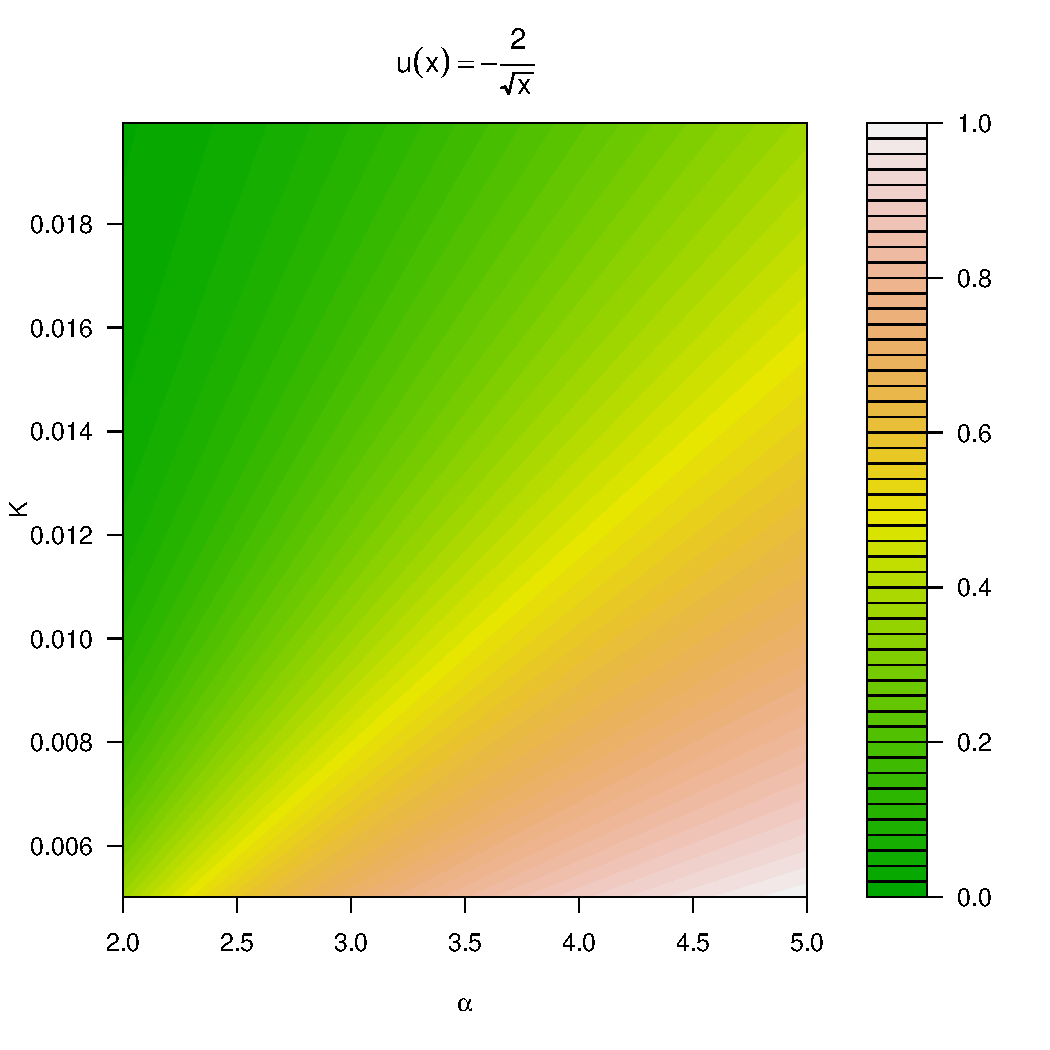
\includegraphics[width=\textwidth]{phi_hat_pareto5e-1_A.pdf}    
  \end{minipage}\hfill
  \begin{minipage}{0.25\linewidth}
    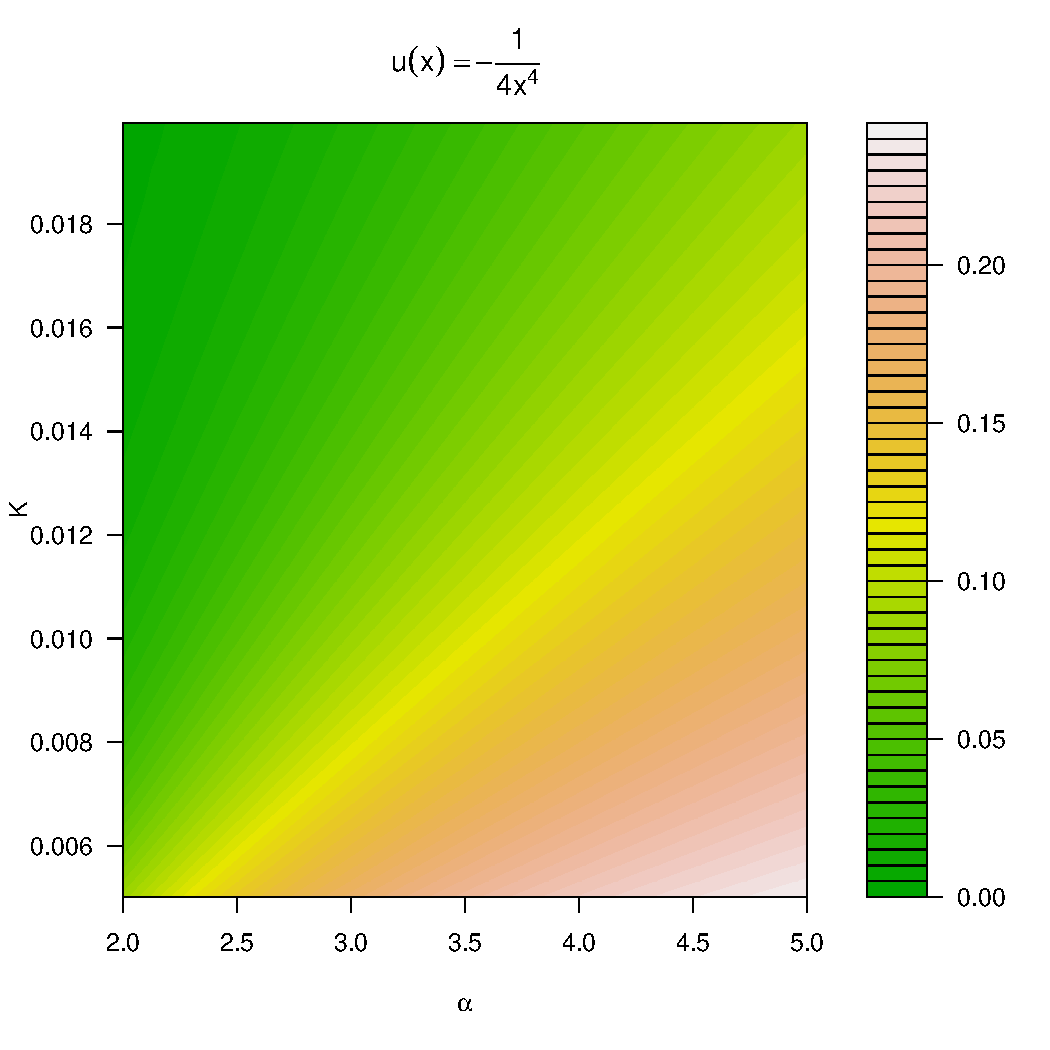
\includegraphics[width=\textwidth]{phi_hat_pareto4_A.pdf}
  \end{minipage}\hfill
  \begin{minipage}{0.25\linewidth}
    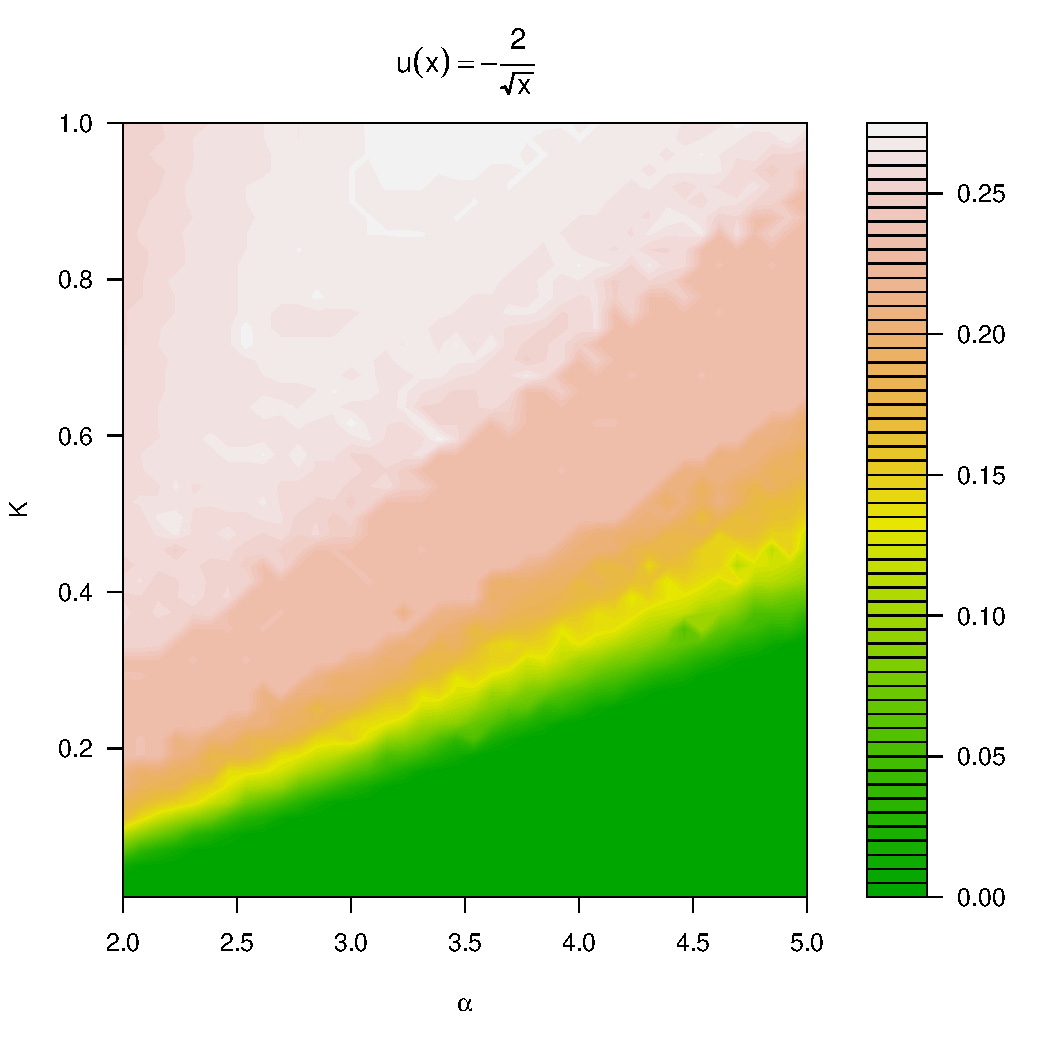
\includegraphics[width=\textwidth]{phi_hat_pareto5e-1.pdf}    
  \end{minipage}\hfill
  \begin{minipage}{0.25\linewidth}
    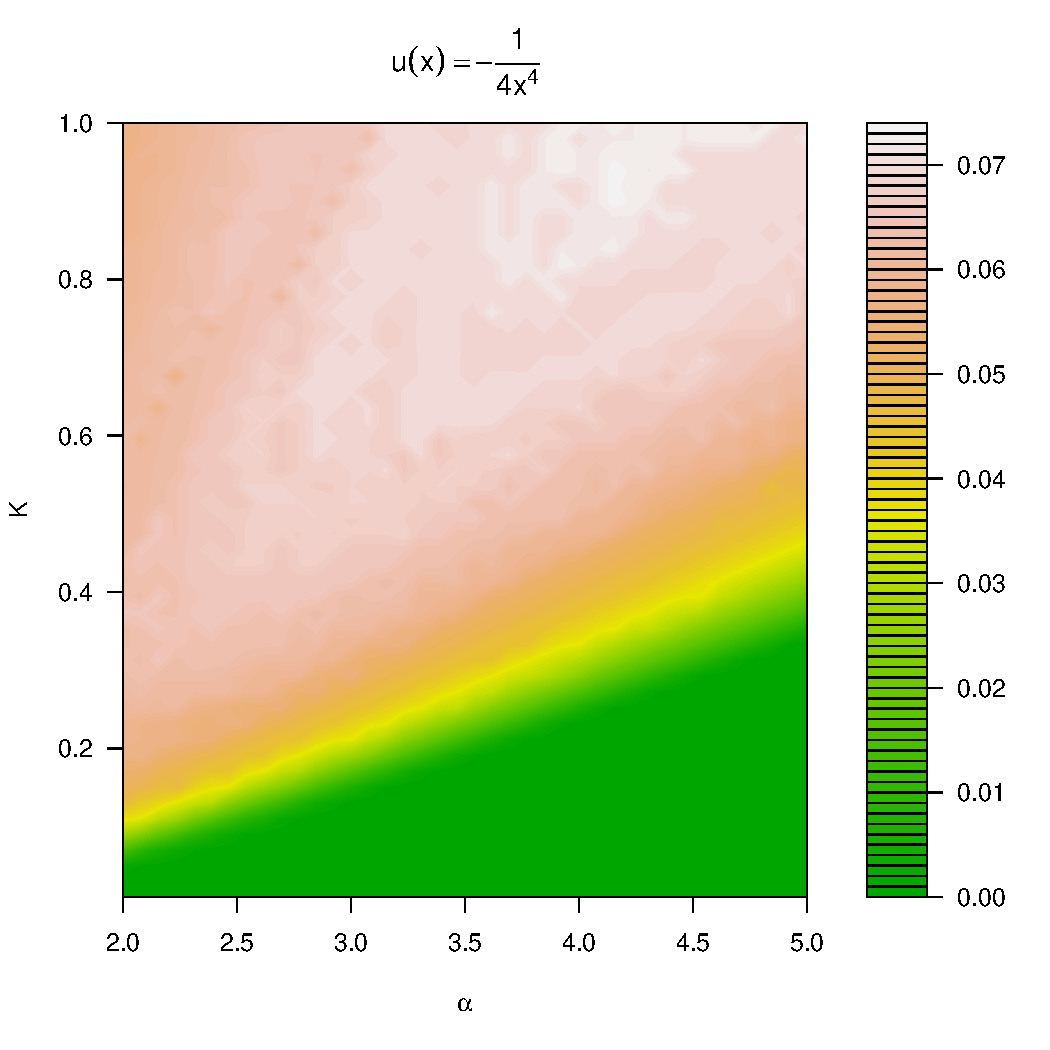
\includegraphics[width=\textwidth]{phi_hat_pareto4.pdf}
  \end{minipage}
 \caption{
   {\em The 1st and 2nd} graphs show $\hat\phi$, the optimal equity
   allocation as a \fct\ of $\alpha$ and $K$ in the two-sided Pareto model
   \eqref{eq:pareto} for fixed $K'=0.012$, $\beta = 1.4$.
   {\em The 3rd and 4th} graphs show $\hat\phi$ as a \fct\ of $\alpha$
   and $K$ with $\beta = \alpha$ and $K' = K$.
   We choose the utility \fct\ $u$ from \eqref{eq:hjyr} for $\xi = 1/2$
   and $\xi = 4$, $b = 0.01$ in all cases.
  }
  \label{fig:phi_hat_pareto}
\end{figure}

\begin{minipage}{0.5\linewidth}
  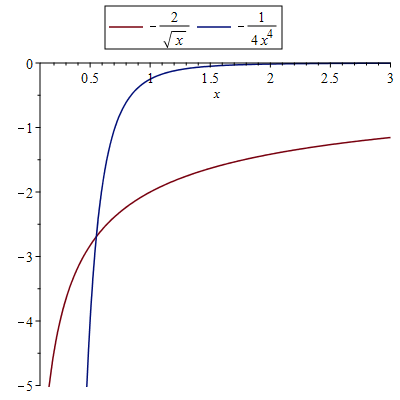
\includegraphics[width=\textwidth]{power_utilities.png}
\end{minipage}\hfill
\begin{minipage}{0.42\textwidth}
  The economitrical differences between the two utility functions
  are illustrated in the graph to the left.
  We see that
  $u(x)$ grows slower and saturates later for small $\xi$ than for
  large $\xi$. The latter case represents an agent who is more
  tolerant about low consumption and seeks wealth more
  aggressively. In other words, he is less risk-averse than one with a
  larger $\xi$. Such an agent will therefore invest more heavily in
  equity, as shown in Figure~\ref{fig:phi_hat_pareto}. Note that,
  while $\hat \phi$ changes nearly in the same way in both graphs, the
  scales in the graphcs are very different.
\end{minipage}

\begin{figure}[htb!]
  \begin{minipage}{0.25\linewidth}
    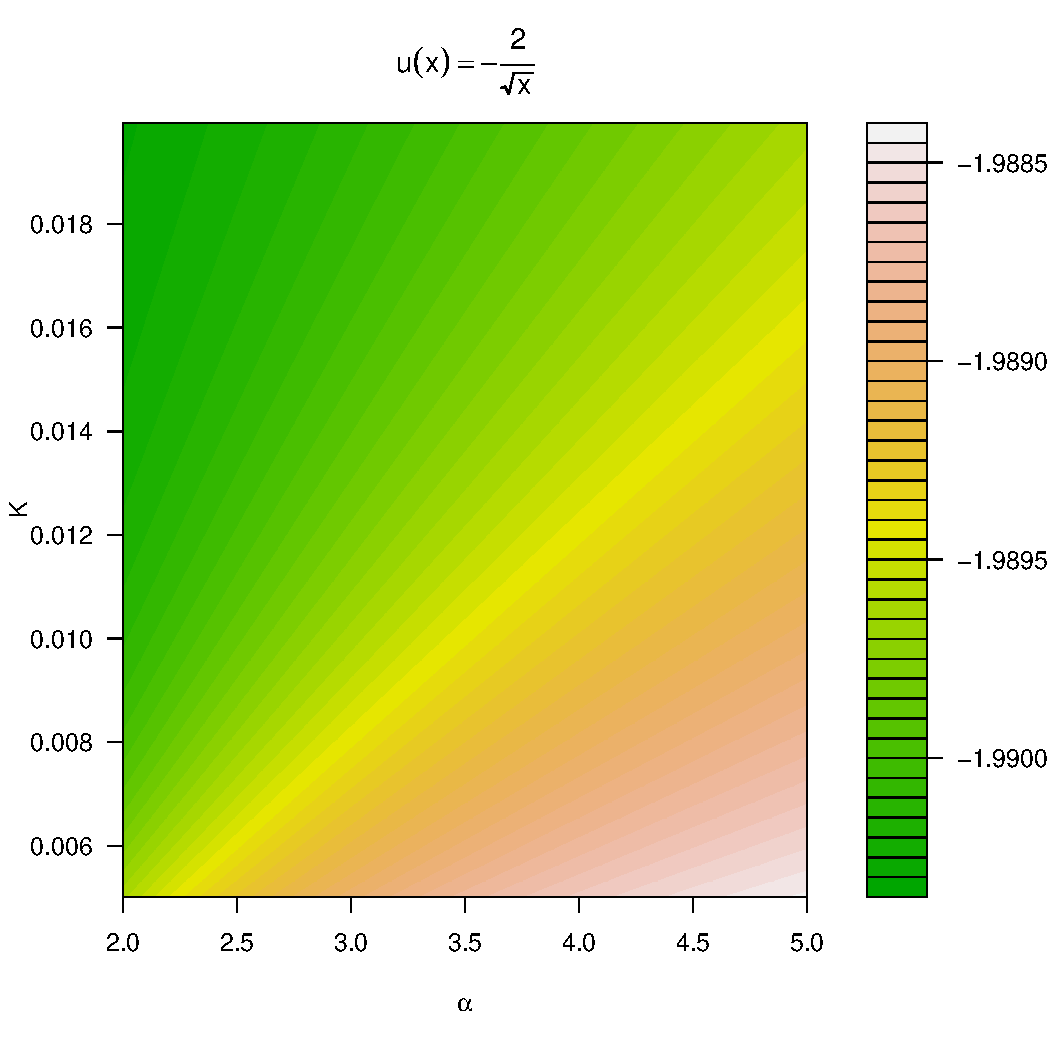
\includegraphics[width=\textwidth]{preference_pareto5e-1_A.pdf}
  \end{minipage}\hfill
  \begin{minipage}{0.25\linewidth}
    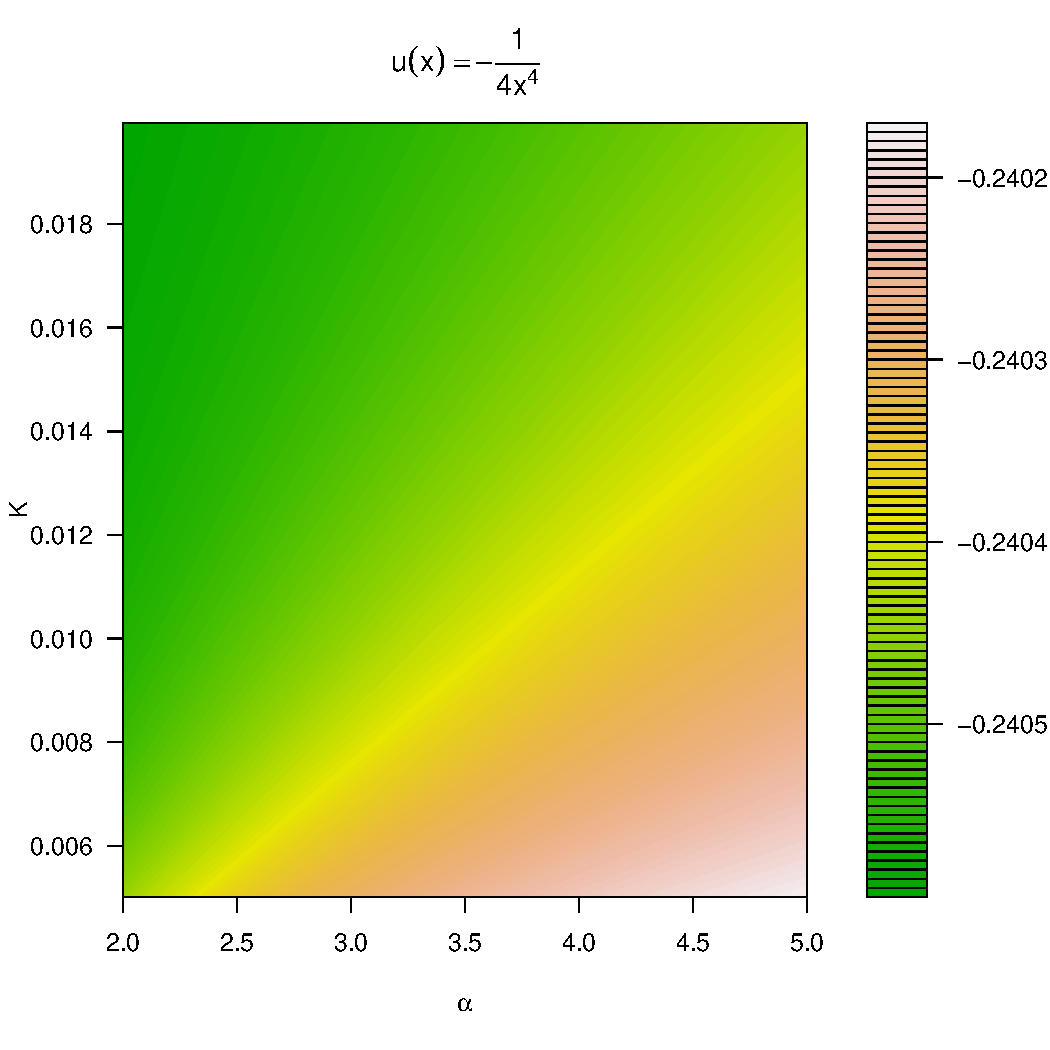
\includegraphics[width=\textwidth]{preference_pareto4_A.pdf}
  \end{minipage}\hfill
  \begin{minipage}{0.25\linewidth}
    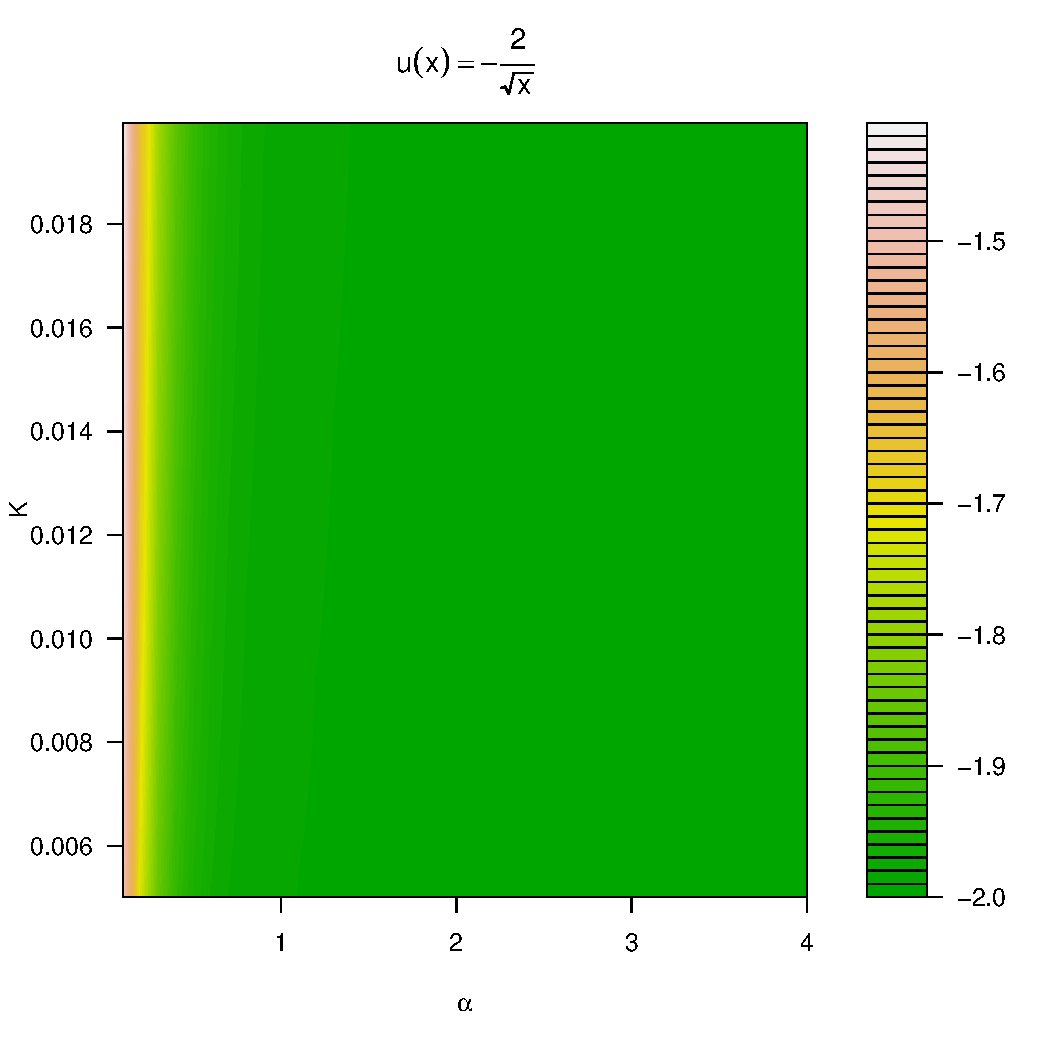
\includegraphics[width=\textwidth]{preference_pareto5e-1.pdf}
  \end{minipage}\hfill
  \begin{minipage}{0.25\linewidth}
    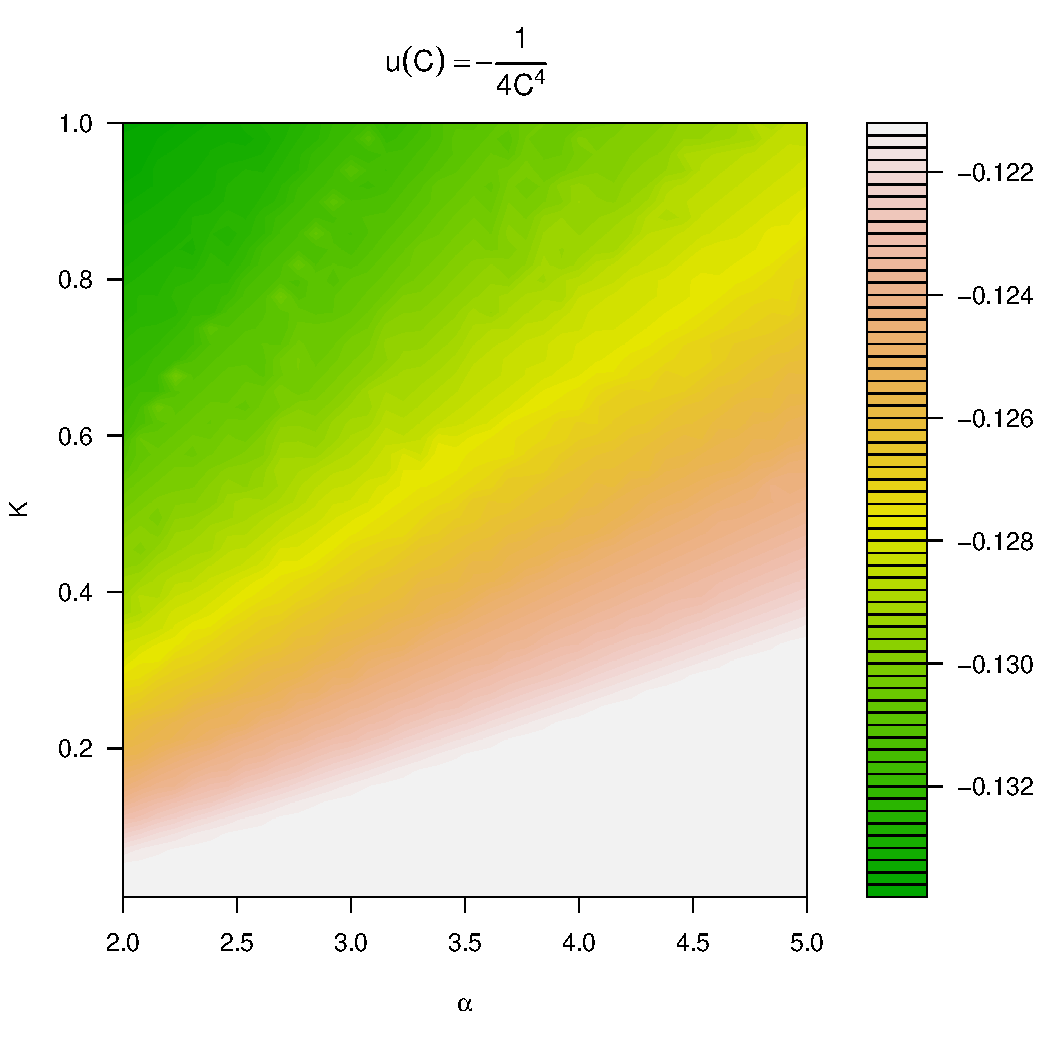
\includegraphics[width=\textwidth]{preference_pareto4.pdf}
  \end{minipage}
  \caption{
   {\em The 1st and 2nd} graphs show
   $\tilde u_{\rm max}(\alpha, K)$, as a \fct\ of $\alpha$ and $K$
   in the two-sided Pareto model \eqref{eq:pareto} with $K'=0.012$,
   $\beta = 1.4$.
   Clearly, $\tilde u_{\rm max}(\alpha, K)$ increases with $\alpha$
   and decreases with $K$ when $K'$ and $\beta$ are fixed.
   {\em The 3rd and 4th} graphs show
   $\tilde u_{\rm max}(\alpha, K)$ as a \fct\ of $\alpha$
   and $K$ with $\beta = \alpha$ and $K' = K$.
   We choose the utility \fct\ $u$ from \eqref{eq:hjyr} for $\xi = 1/2$
   and $\xi = 4$. $b = 0.01$ in all cases.
  }
  \label{fig:preference_pareto}
\end{figure}

If the parameter $b$ is very small the GDA preference is closely
approximated by the mean-utility preference, corresponding to $b = 0$. 
In this case, we show in the proof of Lemma \ref{lemma:III} that the function
$U_{\text{all}}(x)$ may increase or decrease depending on particular conditions
on the values of $\xi$ and $(1 - \phi) e^r / \phi$:
\begin{enumerate}
\item If $\max\{a, 1\} < \xi$, $U_{\text{all}}(\cdot)$ is
  monotone decreasing.
\item If $a < \xi < 1$ and $(a + y_-)/(a y_- + 1) <
  y_-^{(1-\xi)/(1+\xi)}$, $U_{\text{all}}(\cdot)$ is monotone
  decreasing.
\item If $\xi < a < 1$, $U_{\text{all}}(\cdot)$ is monotone
  increasing.
\item If $1 < \xi < a$ and $(a + y_+)/(a y_+ + 1) >
  y_+^{(1-\xi)/(1+\xi)}$, $U_{\text{all}}(\cdot)$ is monotone
  increasing.
\item In other cases, $U_{\text{all}}(\cdot)$ is not monotone.
\end{enumerate}
where
\begin{eqnarray*}
a &=& {
  (1 - \phi) e^r
  \over
  \phi
} \\
y_\pm &=& {
  a^2 - \xi \pm \sqrt{(a^2 - 1) (a^2 - \xi^2)}
  \over
  a (\xi - 1)
}
\end{eqnarray*}
Moreover, it is also easily checked that, when
$x \in (0, K(e^{1/\alpha} - 1)]$,
the density function in the integral of \eqref{eq:ipf} increases
with $\alpha$; when $x \in (K(e^{1/\alpha} - 1), \infty)$ it 
decreases with $\alpha$. Following the arguments for Lemma~\ref{thrm:I},
and applying Lemma \ref{lemma:I}, it can be seen that
$\wt u_{\rm max}(\alpha, K)$ increases/decreases with $\alpha$ when
$U_{\text{all}}(x)$  decreases/increases.

\section{Conclusion}
\label{sec:4}
We have established that, in the case of an equity return series with
two-sided, functionally independent Pareto tails, investor
preference functionals are monotone increasing/decreasing with the
tail index/scale parameters. Thus in a market dominated by such
equities, the investors would pursue the largest tail index in the
market, leading to a shared common tail index for all equities.

The empirical results presented in section \ref{sec:1} suggest this
may well be the case for the ``Consumer Staples'' sector of S\&P 500,
given the Hill estimates of tail indices shown in figure \ref{fig:1}
and the largely positive results of tests for equal tail indices shown
in figure \ref{fig:PairTest}.

On the other hand, we have also seen that, when the left and the right
tails have the same indices, investor preference over the equity has
more sophisticated variations in the parameters' space including the
tail parameters of the equity, the interest rate, the investor's risk
apetite as captured by his utility function, and his threshold of
disappointment.

We also acknowledge that our model of the market and the investor is a
simple one, not accoounting for the dependence between equities, nor
the categorization of investors and their interactions. These are
potential topics of future work.

\ifx\phdthesis\undefined
\appendix
\else
\begin{subappendices}
\fi

\section{A monotonicity lemma}
\setcounter{equation}{0}
\begin{lemma} \label{lemma:I}
  Assume distribution function $F(x, \theta)$ parameterized by 
  $\theta \in \Theta \subseteq \mathbb R$ has support
  $(a, b) \subseteq \mathbb R$,
  and in addition $F(x, \theta)$ has density
  function $f(x, \theta)$ that is differentiable with respect to
  $\theta$ for all $\theta \in \Theta$.
  Let $X \sim F$ and assume function $h(\cdot)$ is defined on $(a, b)$
  and is monotone throughout this interval.
  Moreover, we assume $h(x)$ and $f(x, \theta)$ satisfy
  \begin{equation}\label{eq:frt}
%    \E |h(X)| < \infty, \quad
    \int_a^b \left| {\pd f(x, \theta) \over \pd \theta} \right| dx
    < \infty \text { and }
    \int_a^b \left| h(x) {\pd f(x, \theta) \over \pd \theta} \right| dx
    < \infty
  \end{equation}
  Then the following holds true:
  \begin{enumerate}
  \item If $h(\cdot)$ is decreasing and $\exists x_0 \in (a, b)$ such that
    $\frac{\pd f}{\pd \theta}(x, \theta) > 0$ for $x \in (a, x_0)$ while
    $\frac{\pd f}{\pd \theta}(x, \theta) < 0$ for $x \in (x_0, b)$, then
    \[
    \frac{\pd \E h(X)}{\pd \theta} > 0
    \]
  \item If $h(\cdot)$ is increasing and $\exists x_0 \in (a, b)$ such that 
    $\frac{\pd f}{\pd \theta}(x, \theta) < 0$ for $x \in (a, x_0)$  while
    $\frac{\pd f}{\pd \theta}(x, \theta) > 0$ for $x \in (x_0, b)$, then
    \[
    \frac{\pd \E h(X)}{\pd \theta} > 0
    \]
  \end{enumerate}
\end{lemma}
\begin{remark}
  \label{remark:I}
  Two other cases follow trivially from lemma \ref{lemma:I}:
  \begin{enumerate}
  \item If $h(\cdot)$ is increasing and $\frac{\pd f}{\pd \theta}$
    satisfies the
    same conditions of the 1st case of lemma \ref{lemma:I},
    $\frac{\pd \E h(X)}{\pd \theta} < 0$. This immediately follows
    from applying 1st case of lemma \ref{lemma:I} to $-h(\cdot)$.
  \item By the same argument, if $h(\cdot)$ is decreasing and
    ${\pd f \over \pd \theta}$ satisfies the same conditions of the
    2nd case of lemma \ref{lemma:I}, ${\pd \E h(X) \over \pd \theta} < 0$.
  \end{enumerate}
\end{remark}

\begin{proof}
  Firstly, by dominated convergence theorem, conditions \eqref{eq:frt}
  imply, for all $S \subseteq (a, b)$,
  \begin{eqnarray*}
    {\pd \over \pd \theta}\int_S f(x, \theta) dx
    &=&
    \int_S {\pd \over \pd \theta} f(x, \theta) dx \\
    {\pd \over \pd \theta}\int_S h(x) f(x, \theta) dx
    &=&
    \int_S h(x) {\pd \over \pd \theta} f(x, \theta) dx \\
  \end{eqnarray*}
  Thus we have
  \begin{eqnarray*}
    {\pd \E h(X) \over \pd \theta}
    &=&
    {\pd \over \pd \theta}
    \int_a^b h(x)
    f(x, \theta) dx \\
    &=& \int_a^b h(x)
    {\pd f \over \pd \theta}(x, \theta) dx \\
    &=& \underbrace{\int_a^{x_0}
      h(x) {\pd f \over \pd \theta}(x, \theta) dx}_{I_1}
    + \underbrace{\int_{x_0}^b
      h(x) {\pd f \over \pd \theta}(x,
      \theta) dx}_{I_2}
  \end{eqnarray*}
  $x_0$ being located in the interior of $(a, b)$ and
  $h(\cdot)$ being monotone imply $h(x_0) < \infty$.
  \begin{enumerate}
  \item When $h(x)$ is decreasing on $(a, b)$ and ${\pd f \over \pd
    \theta}(x, \theta) > 0$ on $(a, x_0)$
    \[
    I_1 > h(x_0) \int_a^{x_0}
    {\pd f \over \pd \theta}(x, \theta) dx
    \]
    Similarly, because ${\pd f \over \pd \theta}(x, \theta) < 0$ for
    $x \in (x_0, b)$ and $h(x)$ is decreasing, we have
    \begin{eqnarray*}
      I_2 &=& \int_{x_0}^b -h(x_0)
      \left|{\pd f \over \pd \theta}(x, \theta) \right| dx
      > -h(x_0)
      \int_{x_0}^b \left| 
        {\pd f \over \pd \theta}(x, \theta)
      \right| dx
    \end{eqnarray*}
    Finally we have
    \begin{eqnarray*}
      {\pd \E h(X) \over \pd \theta}
      > h(x_0) \int_a^b
      {\pd f \over \pd \theta}(x, \theta) dx
      = h(x_0) {\partial \over \partial \theta}
      \int_a^b f(x, \theta) dx
      = 0
    \end{eqnarray*}
  \item If $h(\cdot)$ is increasing and $\exists x_0 \in (a, b)$ such that 
    ${\pd f \over \pd \theta}(x_0, \theta) < 0$ on $(a, x_0)$  while
    ${\pd f \over \pd \theta}(x_0, \theta) > 0$ on $(x_0, b)$, 
    by similar arguments, one can show
    \[
    {\pd \E h(X) \over \pd \theta}> 0
    \]
\end{enumerate}
\end{proof}

\section{When equity returns follow Student's t-distribution}
\setcounter{equation}{0}
It is a common practice to use Student's t-distribution to model the
stationary distribution of equity returns. So it is of interest to
find out what implications this distribution has when it is combined
with the PDA preference. Formally we assume
\[
f(x; \alpha) = c(\alpha) \left(
  1 + {x^2 \over \alpha}
\right)^{-(\alpha + 1)/2}
\]
where $\alpha > 1$ and
\[
c(\alpha) = {
  \Gamma({\alpha + 1 \over 2})
  \over
  \Gamma(\alpha/2) \sqrt{\alpha \pi}
}
\]
In the same way as for \eqref{eq:ipf}, we can write $\wt u(F, \phi)$
as
\begin{small}
  \begin{eqnarray}
    \wt u(F, \phi)
    &=&
    (1 + b)
    \int_{0}^{\infty}
    \underbrace{
      \left\{
      u(C(x)) \left[
        1 - {b \over 1 + b}\1_{\{x \ge q\}}
        \right]
      + u(C(-x))
      \right\}
    }_{U_{\text{all}}}
    f(x, \alpha) dx - b u(\delta v) F_X(q)
    \label{eq:t1}
  \end{eqnarray}
\end{small}
where $C(\cdot)$ is defined in \eqref{eq:xxie1}. As shown in lemma
\ref{lemma:III}, when $b = 0$ and $u(\cdot)$
takes the power-form of \eqref{eq:hjyr}, $U_{\text{all}}$ is monotone
depending on the values of $\xi$ and $(1 - \phi) e^r / \phi$. As given
in lemma \ref{lemma:II}, there is a point $x_0 > 0$ such that
${\pd f \over \pd \alpha}(x_0, \alpha) = 0$ and
$\forall x \in (0, x_0),
{\pd f \over  \pd \alpha}(x, \alpha) > 0$ and
$\forall x \in (x_0, \infty)$,
${\pd f \over \pd \alpha}(x, \alpha) < 0$. Thus it remains to verify
$\int_0^\infty |{\pd f \over \pd \alpha}(x, \alpha)| dx < \infty$ and
$\int_0^\infty |U_{\text{all}}(x){\pd f \over \pd \alpha}(x, \alpha)| dx < \infty$
if we are to apply lemma \ref{lemma:I}.

As computed in the proof of lemma \ref{lemma:II}, ${\pd f \over \pd
  \alpha}(x, \alpha)$ is given by \eqref{eq:xxie4.1}. It is also shown
there ${d \over d \alpha} c(\alpha) > 0$. Thus for
$\int_0^\infty |{\pd f \over \pd \alpha}(x, \alpha)| dx < \infty$
it suffices to show
\[
\int_ 0^\infty {
x^2
\over
(x^2 + \alpha) (1 + x^2 / \alpha)^{\alpha/2 + 1/2}
} dx < \infty
\]
We may write
\begin{eqnarray*}
&& \int_ 0^\infty {
x^2
\over
(x^2 + \alpha) (1 + x^2 / \alpha)^{\alpha/2 + 1/2}
} dx \\
&=& \left(\int_0^1 + \int_1^\infty \right) {
x^2
\over
(x^2 + \alpha) (1 + x^2 / \alpha)^{\alpha/2 + 1/2}
} dx \\
&=& I_1 + I_2
\end{eqnarray*}
Clearly
\[
I_1 < \int_0^1 {1 \over \alpha} dx < \infty
\]
while
\begin{eqnarray*}
  I_2 &=& \int_1^\infty {1 \over 1 + \alpha/x^2}
  {1 \over (1/x^2 + 1/\alpha)^{(\alpha+1) / 2}} {dx \over x^{\alpha +
      1}} \\
  &<& \int_1^\infty \alpha^{(\alpha+1) / 2} {dx \over x^{\alpha + 1}}
  < \infty
\end{eqnarray*}
So we conclude
$\int_0^\infty |{\pd f \over \pd \alpha}(x, \alpha)| dx < \infty$.
To see
$\int_0^\infty |U_{\text{all}}(x){\pd f \over \pd \alpha}(x, \alpha)| dx < \infty$, we note
\begin{eqnarray*}
  \xi |U_{\text{all}}(x)|
  &<& [(1 - \phi) e^r + e^x]^{-\xi} + [(1 - \phi) e^r + e^{-x}]^{-\xi} \\
  &<& 1 + (1 - \phi)^{-\xi} e^{-r \xi}
\end{eqnarray*}
Since $\int_0^\infty |{\pd f \over \pd \alpha}(x, \alpha)| dx < \infty$,
it follows from the above inequality $\int_0^\infty |U_{\text{all}}(x){\pd f \over \pd \alpha}(x, \alpha)| dx < \infty$.
Thus by lemma \ref{lemma:I}, $\wt u_{\rm max}$ is monotone
increasing/decreasing with $\alpha$ when $U_{\text{all}}(\cdot)$ is
monotone decreasing/increasing. Accordingly, an investor guided by the
utility function will seek the largest/smallest $\alpha$ observed in
the market.

If however $b > 0$, Lemma \ref{lemma:I} is not applicable
anymore. Nonetheless, numerical analysis lends some insight.
As shown in figure \ref{fig:htfg}, $\hat\phi$ is monotone increasing
for all 4 values of $b$, while $\tilde u_{\rm max}(\alpha)$ is
increasing with $\alpha$ when $b$ is relatively large, but
decreasing with $\alpha$ when $b$ is small. We note that a sizable
value of $b$ indicates a conservative, risk-averse investor.

\begin{figure}[htb!]
  \begin{minipage}{0.5\linewidth}
    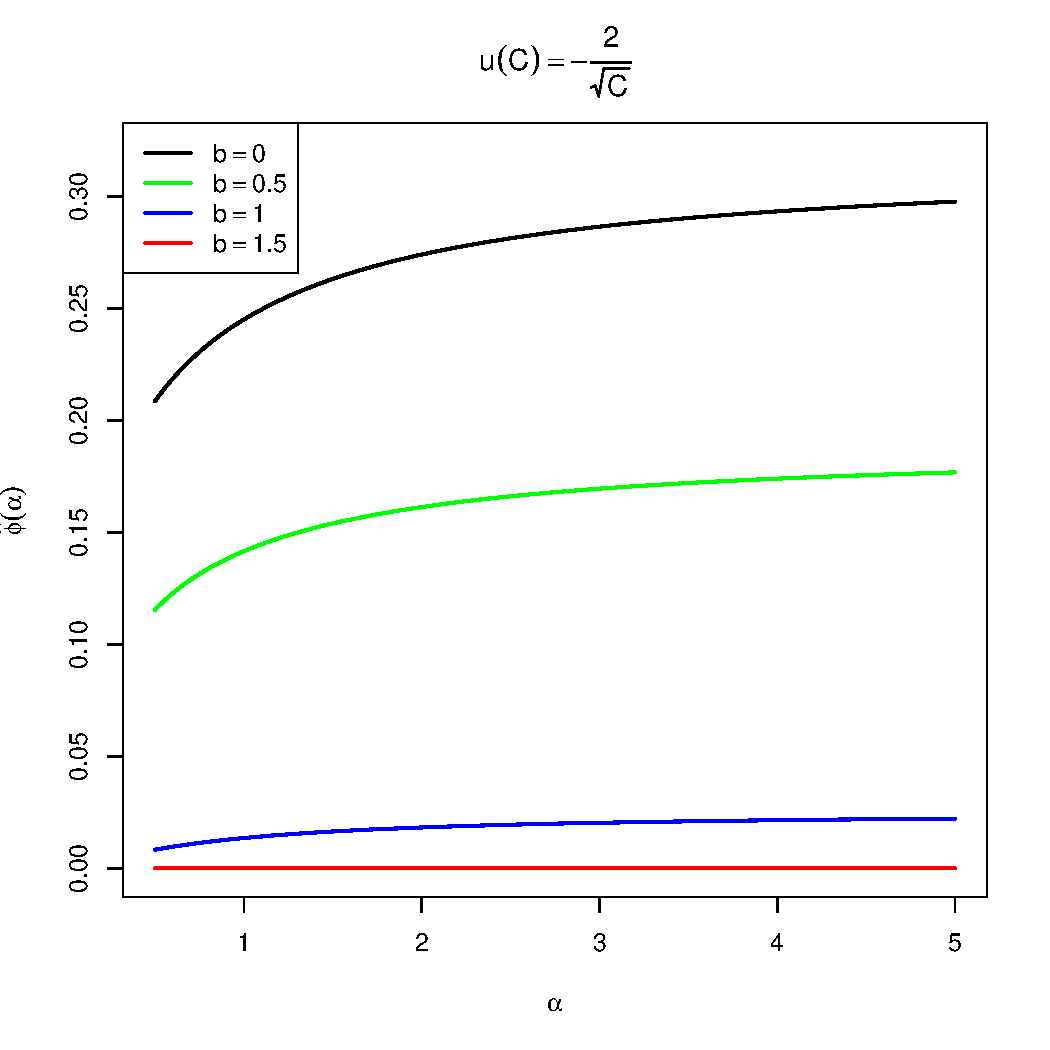
\includegraphics[width=\textwidth]{phi_hat_b_t_power.pdf}
  \end{minipage}\hfill
  \begin{minipage}{0.5\linewidth}
    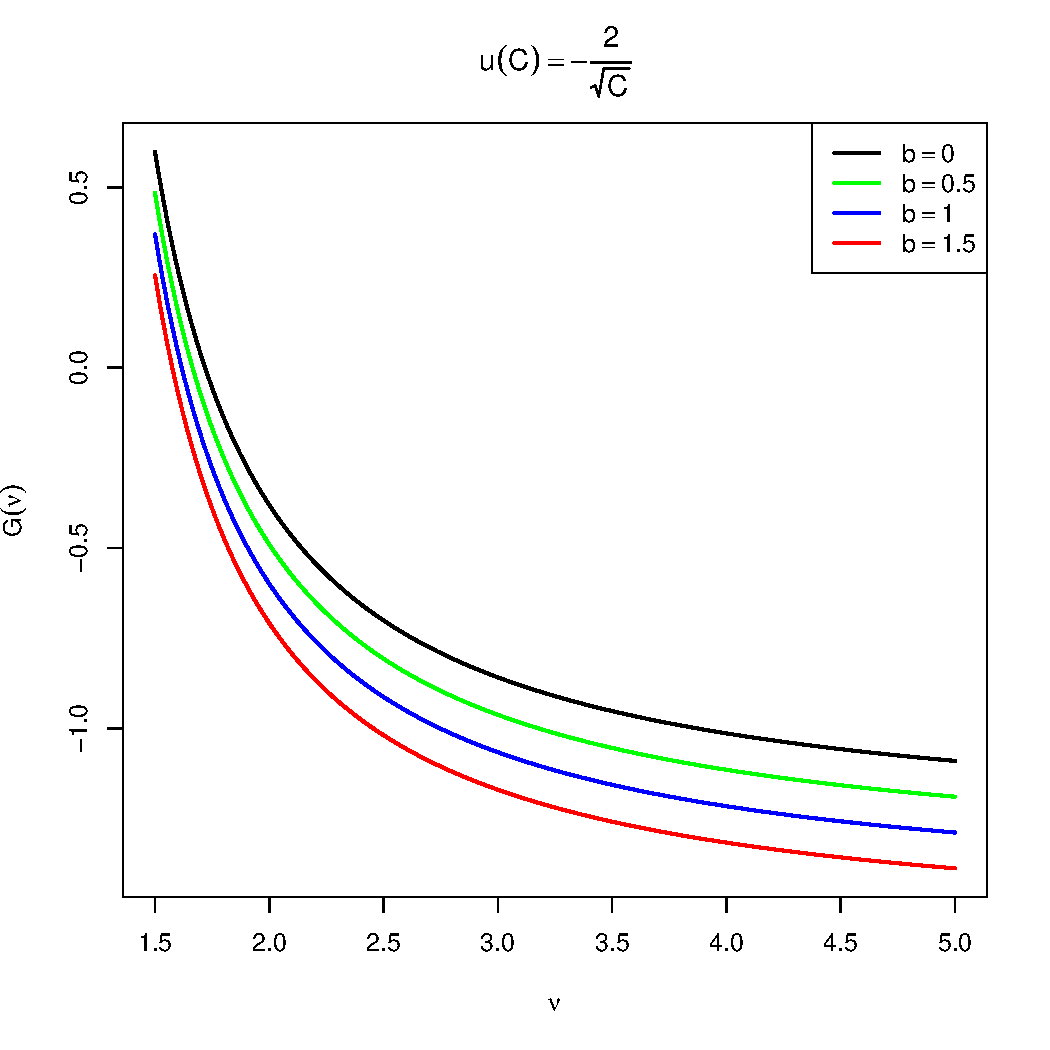
\includegraphics[width=\textwidth]{U_b_t_power.pdf}
  \end{minipage}
  \begin{minipage}{0.5\linewidth}
    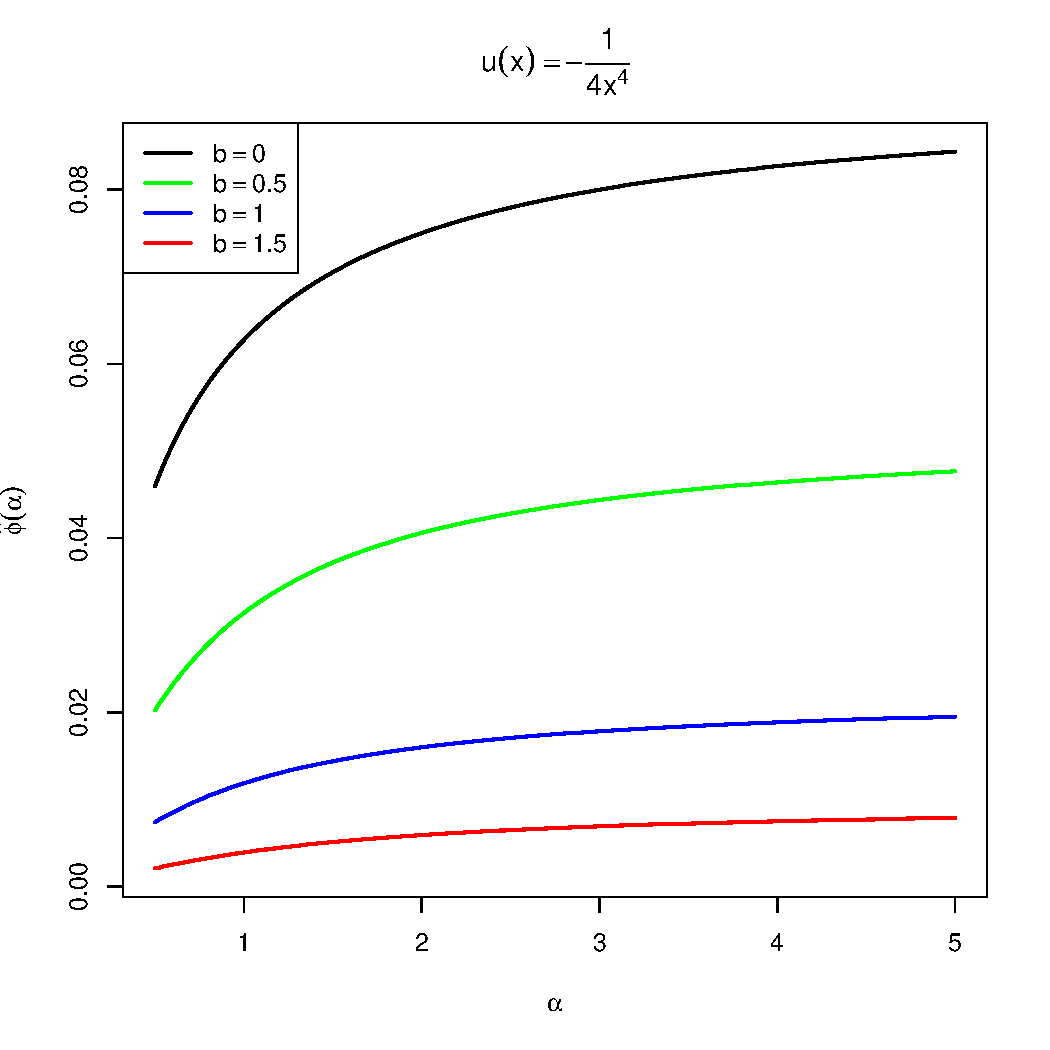
\includegraphics[width=\textwidth]{phi_hat_b_t_power4.pdf}
  \end{minipage}\hfill
  \begin{minipage}{0.5\linewidth}
    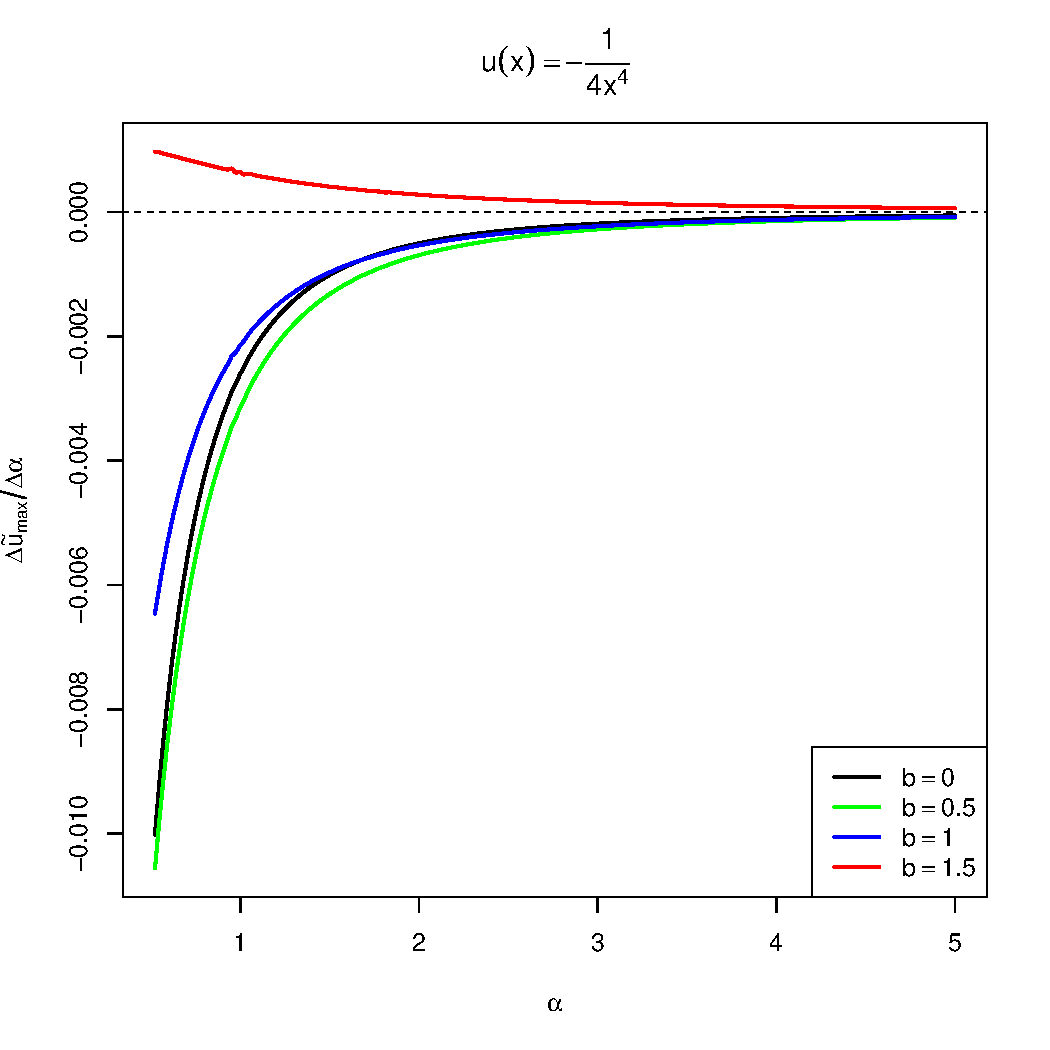
\includegraphics[width=\textwidth]{U_b_t_power4.pdf}
  \end{minipage}
  \caption{$\hat\phi$ (left) and ${\pd \tilde u_{\rm max} \over \pd
      \alpha}$ (right). {\em top:} $\xi = 1/2$. {\em bottom:} $\xi =
    4$.
  }
  \label{fig:htfg}
\end{figure}
\begin{lemma}
  \label{lemma:II}
  Let $f$ denotes the density function of the Student's
  t-distribution, i.e.
  \[
  f(x; \alpha) = c(\alpha) \left(
    1 + {x^2 \over \alpha}
  \right)^{-(\alpha + 1)/2}
  \]
  where $\alpha > 1$ and
  \[
  c(\alpha) = {
    \Gamma({\alpha + 1 \over 2})
    \over
    \Gamma(\alpha/2) \sqrt{\alpha \pi}
  }
  \]
  Then there exists $x_0 > 0$ such that ${\pd f \over
    \pd \alpha}(x_0, \alpha) = 0$ and $\forall x \in (0, x_0), {\pd f \over
    \pd \alpha}(x, \alpha) > 0$ and $\forall x \in (x_0, \infty), {\pd f
    \over \pd \alpha}(x, \alpha) < 0$.
\end{lemma}
\begin{proof}
  Straightforward computation gives
  \begin{eqnarray}
    {\pd f(x, \alpha) \over \pd \alpha} &=& {
      c(\alpha) x^2 (\alpha + 1) + (2 \alpha x^2 + 2 \alpha^2) c'(\alpha)
      -
      \alpha c(\alpha) (x^2 + \alpha) \log(1 + x^2/\alpha)
      \over
      2 \alpha (x^2 + \alpha) (1 + x^2 / \alpha)^{\alpha/2 + 1/2}
    } \nonumber \\
    &:=& {
      P(x^2, \alpha)
      \over
      2 \alpha (x^2 + \alpha) (1 + x^2 / \alpha)^{\alpha/2 + 1/2}
    }
    \label{eq:xxie4.1}
  \end{eqnarray}

  While the denominator of the right side of ${\pd f(x, \alpha) \over \pd \alpha}$ is
  always positive, its numerator $P(x^2, \alpha)$ has a single root:
  \begin{equation}
    \label{eq:xxie5}
    x_0^2 = \alpha\exp\left\{
      W\left[
        -\left(1 + {1 \over \alpha}\right)
        e^{-1 - 2 c'(\alpha)/c(\alpha) - 1/\alpha}
      \right]
      + 1 + {1 \over \alpha} + {2 c'(\alpha) \over c(\alpha)}
    \right\} - \alpha
  \end{equation}
  where $W(\cdot)$ is the principle branch of the Lambert $W$
  function. and $c'(\cdot)$ is the derivative of $c(\cdot)$. To check
  the right side of \eqref{eq:xxie5} for positivity, we first note
  $c'(\alpha) > 0$:
  \[
  c'(\alpha) = {
    \pi \Gamma(\alpha/2 + 1/2) \left\{
      \alpha \left[ \Psi(\alpha/2 + 1/2) - \Psi(\alpha/2)\right] - 1
    \right\}
    \over
    2 \Gamma(\alpha/2) (\pi \alpha)^{3/2}
  }
  \]
  where $\Psi(\cdot)$ is the digamma function:
  \[
  \Psi(x) = {d \log[\Gamma(x)] \over d x}
  \]
  \begin{minipage}{0.48\textwidth}
    $\Psi(x)$ \linebreak
    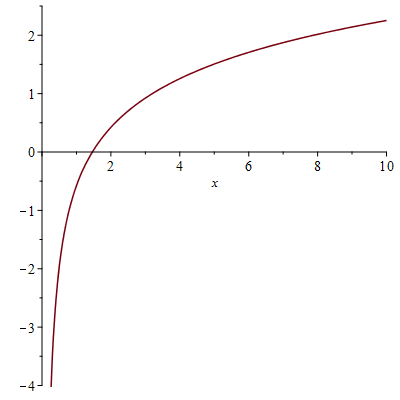
\includegraphics[width=\textwidth]{digamma.png}
  \end{minipage}\hfill
  \begin{minipage}{0.5\textwidth}
    As shown in the figure to the left, $\Psi(x)$ is increasing
    for $x > 0$. This immediately follows from the series
    representation
    \[
    \Psi(x + 1) = -\gamma + \sum_{n=1}^\infty {x \over n(n + x)}
    \quad x \neq -1, -2, -3,\dots
    \]
    which gives
    \[
    {\pd \Psi(x + 1) \over \pd x}
    = \sum_{n=1}^\infty {1 \over (n + x)^2} > 0
    \]
    See Abramowitz and Stegun \cite{abramowitz1972handbook}, p.259,
    formula 6.3.16. Therefore $\Psi(\alpha/2 + 1/2) - \Psi(\alpha/2) > 0$.
    So we have
    \begin{eqnarray*}
      && \alpha \left[
        \Psi(\alpha/2 + 1/2) - \Psi(\alpha/2)
      \right] - 1 \\
      &\geq& 1 \times \left[
        \Psi(1/2 + 1/2) - \Psi(1/2)
      \right] - 1 \\
      &=& \log(4) - \log(e) \\
      &>& 0
    \end{eqnarray*}
    Thus $c'(\alpha) > 0$. Furthermore, we recall
    $W(\cdot)$ is increasing on its principle branch. So
  \end{minipage}
  \begin{eqnarray*}
    &&
    W\left[
      -\left( 1 + {1 \over \alpha} \right)
      e^{-1 - 2 c'(\alpha)/c(\alpha) - 1/\alpha}
    \right]
    + 1 + {1 \over \alpha} + {2 c'(\alpha) \over c(\alpha)} \\
    &>& 
    W\left[
      -\left( 1 + {1 \over \alpha} + {2 c'(\alpha) \over c(\alpha)} \right)
      e^{-1 - 2 c'(\alpha)/c(\alpha) - 1/\alpha}
    \right]
    + 1 + {1 \over \alpha} + {2 c'(\alpha) \over c(\alpha)} \\
    &=& W(-y e^{-y}) + y
  \end{eqnarray*}
  where
  \[
  y = 1 + {1 \over \alpha} + {2 c'(\alpha) \over c(\alpha)} > 1
  \]
  Now notice
  \[
  \log(y e^{-y}) = \log(y) - y
  \]
  is a decreasing function for $y > 1$. Thus $-y e^{-y}$ is an
  increasing function. Hence we have
  \begin{eqnarray*}
    W(-y e^{-y}) + y &>& W(-e^{-1}) + 1 = 0
  \end{eqnarray*}
  Now it is clear
  \[
  \alpha\exp\left\{
    W\left[
      -\left(1 + {1 \over \alpha}\right)
      e^{-1 - 2 c'(\alpha)/c(\alpha) - 1/\alpha}
    \right]
    + 1 + {1 \over \alpha} + {2 c'(\alpha) \over c(\alpha)}
  \right\} - \alpha > 0
  \]
  Now that we have established that ${\pd f \over \pd \alpha}(x,
  \alpha) = 0$ has a single positive root, it remains to determine the
  sign of ${\pd f \over \pd \alpha}(x, \alpha)$ on the two sides of
  the root. For this purpose we observe
  \begin{equation}
    \label{eq:xxie5.1}
    P(0, \alpha) = 2 \alpha^2 c'(\alpha) > 0
  \end{equation}
  So we want to investigate ${\pd P \over \pd x}(x, \alpha)$:
  \begin{eqnarray}
    {\pd P \over \pd x}(x, \alpha) &=&
    2 \alpha c'(\alpha) + c(\alpha) - \alpha c(\alpha) \log\left(
      1 + {x \over \alpha}
    \right)
    \label{eq:xxie6}
  \end{eqnarray}
  Clearly, $\frac{\pd P}{\pd x}(0, \alpha) > 0$. Hence from
  \eqref{eq:xxie5.1} and
  \eqref{eq:xxie6} it is clear
  \begin{equation*}
    \text{sign}\left[
      {\pd f \over \pd\alpha}(x, \alpha)
    \right]
    = \left\{
    \begin{array}{rl}
      1 & 0 < x < x_0 \\
      -1 & x > x_0
    \end{array}
    \right.
  \end{equation*}
  where $x_0$ is the positive root of \eqref{eq:xxie5}.
\end{proof}

\section{Proof of Lemma~\ref{thrm:I}}
\setcounter{equation}{0}
\label{sec:thrmI_proof}
\begin{proof}
  Let
  \begin{equation}
    \label{eq:xxie2}
    \hat \phi := \underset{0 < \phi \leq 1}{\text{argmax}}\,
    \wt u(F_X, \phi)
  \end{equation}
  We have
  \[
  \tilde u_{\rm max}(F_X) = \wt u(F_X, \hat\phi)
  \]
  It follows
  \begin{eqnarray}
    {d \tilde u_{\rm max}(F_X) \over d \alpha}
    &=&
    \left.{\pd \wt u(\alpha, \phi) \over \pd \alpha}\right|_{\phi = \hat\phi}
    + \left.{\pd \wt u(\alpha, \phi) \over \pd \phi}\right|_{\phi = \hat\phi}
    {\pd \hat\phi \over \pd \alpha}
    \label{eq:xxie3}
  \end{eqnarray}
  The definition \eqref{eq:xxie2} implies for all $\alpha$
  \begin{equation}
    \label{eq:xxie4}
    \left.{\pd \wt u(\alpha, \phi) \over \pd \phi}\right|_{\phi = \hat\phi} = 0
  \end{equation}
  So the second term of \eqref{eq:xxie3} vanishes. It remains to show
  the first term is positive. From \eqref{eq:xxie1.0}, it follows
  \begin{eqnarray*}
    {\pd \wt u(\alpha, \phi) \over \pd \alpha}
    = {\partial \over \partial \alpha}\E[u((1 - \phi) e^r + \phi e^x) \1_{\{X < 0\}}]
  \end{eqnarray*}
  The function $u((1 - \phi) e^r + \phi e^x)$ is obviously
  increasing with $x$. It follows
  \begin{eqnarray*}
    {\pd f_X(x; \alpha, K) \over \pd \alpha}
    = {\partial \over \partial \alpha} {\alpha K^\alpha \over (K - x)^{\alpha + 1}} 
    = - {K^\alpha \over (K - x)^{\alpha + 1}}
    \left[
      \alpha
      \log\left(
        1 - {x \over K}
      \right) - 1
    \right]
  \end{eqnarray*}
  It is easily checked
  \[
  {\partial \over \partial \alpha}
  {\alpha K^\alpha \over (K - x)^{\alpha + 1}}
  \left\{
    \begin{array}{ll}
      > 0 & \text{ when } x < K(1 - e^{1/\alpha}) < 0 \\
      < 0 & \text{ when } K(1 - e^{1/\alpha}) < x < 0
    \end{array}
  \right.
  \]
% that when $x < K(1 - e^{1/\alpha}) < 0$,
%   \[
%   {\partial \over \partial \alpha} {\alpha K^\alpha \over (K - x)^{\alpha + 1}} < 0
%   \]
%   and when $K(1 - e^{1/\alpha}) < x < 0$,
%   \[
%   {\partial \over \partial \alpha} {\alpha K^\alpha \over (K - x)^{\alpha + 1}} > 0
%   \]
  This is the second case of lemma \ref{lemma:I}. So we have
  ${\pd \wt u(\alpha, \phi) \over \pd \alpha} > 0$.
  As for ${\pd \tilde u_{\rm max}(F_X) \over \pd K}$, by the same
  argument, it suffices to show ${\pd \wt u(K, \phi) \over \pd K} < 0$.
  We have
  \[
  {\pd \wt u(K, \phi) \over \pd K}
  = {\partial \over \partial K} \E \left[
    u((1 - \phi) e^r + \phi e^x) \1_{\{X < 0\}}
  \right] 
  \]
  and
  \begin{eqnarray*}
    {\pd f_X(x; \alpha, K) \over \pd K}
    = {\partial \over \partial K} {\alpha K^\alpha \over (K - x)^{\alpha + 1}}
   = -\alpha K^{\alpha - 1} {
      \alpha x + K
      \over
      (K - x)^{\alpha + 2}
    }
  \end{eqnarray*}
  Clearly,
  \[
  {\partial \over \partial K}
  {\alpha K^\alpha \over (K - x)^{\alpha + 1}}
  \left\{
    \begin{array}{ll}
      > 0 & \text{ when } x < -K/\alpha < 0\\
      < 0 & \text{ when } -K/\alpha < x < 0
    \end{array}
  \right.
  \]
  % Clearly, when $x < -K/\alpha$
  % \[
  % {\partial \over \partial K} {\alpha K^\alpha \over (K - x)^{\alpha + 1}} > 0
  % \]
  % and when $-K/\alpha < x < 0$
  % \[
  % {\partial \over \partial K} {\alpha K^\alpha \over (K - x)^{\alpha + 1}} < 0
  % \]
  So by the 1st case of Remark \ref{remark:I} we conclude $  {\pd \wt u(K, \phi) \over \pd K} < 0$.
\end{proof}

\section{Lemma~\ref{lemma:III}}
\setcounter{equation}{0}
\begin{lemma}\label{lemma:III}
Let $u(\cdot)$  and $C(\cdot)$ be defined as in \eqref{eq:hjyr} and
\eqref{eq:xxie1} respectively. Define
\begin{eqnarray*}
U_{\text{all}} &=& u(C(x))
+ u(C(-x))
\quad
x \geq 0 \\
a &=& {
  (1 - \phi) e^r
  \over
  \phi
} \\
y_\pm &=& {
  a^2 - \xi \pm \sqrt{(a^2 - 1) (a^2 - \xi^2)}
  \over
  a (\xi - 1)
}
\end{eqnarray*}
The following holds true:
\begin{enumerate}
\item If $\max\{a, 1\} < \xi$, $U_{\text{all}}(\cdot)$ is
  monotone decreasing.
\item If $a < \xi < 1$ and $(a + y_-)/(a y_- + 1) <
  y_-^{(1-\xi)/(1+\xi)}$, $U_{\text{all}}(\cdot)$ is monotone
  decreasing.
\item If $\xi < a < 1$, $U_{\text{all}}(\cdot)$ is monotone
  increasing.
\item If $1 < \xi < a$ and $(a + y_+)/(a y_+ + 1) >
  y_+^{(1-\xi)/(1+\xi)}$, $U_{\text{all}}(\cdot)$ is monotone
  increasing.
\item In other case, $U_{\text{all}}(\cdot)$ is not monotone.
\end{enumerate}
\end{lemma}
\begin{proof}
  It is convenient to re-write $U_{\text{all}}$ as
  \[
  U_{\text{all}} =
  -{\phi^{-\xi} \over \xi} \left\{
    \underbrace{
      \left[{(1 - \phi) \over \phi} e^r + e^x\right]^{-\xi}
      +
      \left[{(1 - \phi) \over \phi} e^r + e^{-x}\right]^{-\xi}
    }_{U(x)}
  \right\}
  \]
  Thus the monotonicity of $U_{\text{all}}(x)$ is the opposite of $U(x)$. For
  convenience of writing, let $a = (1 - \phi)e^r/\phi$.
  First of all, we find the conditions on which $U(x)$ is monotone.
  Direct differentiation yields
  \begin{eqnarray*}
    {\pd U(x) \over \pd x}
    &=&
    -{
      (a + e^x)^{-\xi - 1} \xi e^x
    } + (a + e^{-x})^{-\xi - 1} \xi e^{-x}
  \end{eqnarray*}
  ${\pd U(x) \over \pd x} = 0$ is equivalent to
  \begin{eqnarray*}
    {a + y \over a y + 1} &=& y^{1 -\xi \over 1+\xi} \\
    \underbrace{\log(a + y) - \log(a y + 1)}_{f(y)} &=&
    {1 -\xi \over 1+\xi} \log(y)
  \end{eqnarray*}
  where we have defined $y = e^x$, and $f(y)$, $g(y)$ as above. Observe
  \begin{equation}
    \label{eq:f-g-der}
    {\pd (f -g)(y) \over \pd y} = {
      a (\xi - 1) y^2 + 2 (\xi - a^2) y + a(\xi - 1)
      \over
      (1 + \xi) (a + y) (a y + 1) y
    }
  \end{equation}
  ${\pd (f -g)(y) \over \pd y} = 0$ has two roots when $\xi \ne 1$
  \begin{eqnarray*}
    y_\pm &=& {
      a^2 - \xi \pm \sqrt{(a^2 - 1) (a^2 - \xi^2)}
      \over
      a (\xi - 1)
    }
  \end{eqnarray*}
  \begin{enumerate}
  \item If $\min\{1, \xi\} < a < \max\{1, \xi\}$, $y_\pm$ are not
    real, ${\pd (f -g)(y) \over \pd y} = 0$ has no solution on
    $(1, \infty)$; $(f -g)(y)$ is monotone on $(1, \infty)$.
    \begin{enumerate}
    \item If in addition $\xi > 1$, i.e. $1 < a < \xi$, $(f - g)(y)$
      is monotone increasing on $(1, \infty)$, because the
      coefficient of the $y^2$ term of the numerator of
      \eqref{eq:f-g-der}, i.e. $a (\xi - 1)$ is positive. We note
      $f(1) = g(1) = 0$; thus on $(1, \infty)$, there is no solution
      to $f(y) = g(y)$. It can be concluded that $U(\cdot)$ is
      monotone on $(0, \infty)$. Furthermore
        \begin{eqnarray*}
          \left.{\pd U(x) \over \pd x}\right|_{x=0} &=& 0 \\
        \end{eqnarray*}
        For a small $\epsilon > 0$, the sign of ${\pd U(x) \over \pd
          x}$ on $(0, \epsilon)$ is thus the same as
        $\left.{\pd^2 U(x) \over \pd x^2}\right|_{x=0}$:
        \[
        \left.{\pd^2 U(x) \over \pd x^2}\right|_{x=0} =
        2 (a + 1)^{-\xi - 2} (\xi - a) > 0
        \]
        Thus ${\pd U(x) \over \pd x} > 0$ for $x \in (0, \infty)$;
        $U_{\text{all}}$ is monotone decreasing.
    \item If instead $\xi < 1$, i.e. $\xi < a < 1$, by a similar
      argument as in the previous case, $U_{\text{all}}$ is monotone
      increasing on $(0, \infty)$.
    \end{enumerate}
  \item If $a < \min\{1, \xi\}$ and $\xi > 1$, i.e. $a < 1 < \xi$, it
    is clear
    \[
    y_- = {
      a^2 - \xi - \sqrt{(a^2 - 1) (a^2 - \xi^2)}
      \over
      a (\xi - 1)
    } < 0
    \]
    It remains to compare $y_+$ with $1$ to determine whether
    ${\pd (f -g)(y) \over \pd y} = 0$ has a solution on $(1, \infty)$.
    Assume $y_+ > 1$. Then
    \begin{eqnarray}
      a^2 - \xi + \sqrt{(a^2 - 1) (a^2 - \xi^2)} &>& a (\xi - 1)
      \nonumber \\
      2 a (\xi - 1) (a + 1) (a - \xi) &>& 0 \label{eq:mi6}
    \end{eqnarray}
    This contradicts the assumption $a < \xi$ and $\xi > 1$. Hence
    $y_+ < 1$. So we conclude $(f - g)(y)$ is monotone increasing
    on $(1, \infty)$. Following the same analysis as in the case
    (1.a), one can see $U_{\text{all}}$ is monotone decreasing.

  \item If $a < \min\{1, \xi\}$ and $\xi < 1$, i.e. $a < \xi < 1$, it
    is clear $y_- > 0$ and $y_+ < y_-$. Moreover, $y_- > 1$ is equivalent
    to
    \[
    \sqrt{(a^2 - 1) (a^2 - \xi^2)} > a^2 - \xi a + a - \xi
    = (a + 1) (a - \xi)
    \]
    The last inequality is obviously true in this case. So $y_- >
    1$. ${\pd (f-g)(y) \over \pd y}$ has a maximum at
    $y_- \in (1, \infty)$. We know $(f - g)(y_-)$ is a maximum because
    \eqref{eq:f-g-der} shows that, for $y > y_-$,
    ${\pd (f-g)(y) \over \pd y} < 0$.

    If $(f-g)(y_-) < 0$, $(f-g)(y) = 0$ has no solution on $(1,
    \infty)$. Hence $U(\cdot)$ is monotone on both $(0, \infty)$.
    The same analysis as in the case (1.a) shows $U_{\text{all}}$
    is monotone decreasing on $(0, \infty)$.

    If $(f-g)(y_-) > 0$, $(f-g)(y) = 0$ must have a solution on $(y_-,
    \infty)$. So $U(\cdot)$ is not monotone.

    \item $a > \max\{1, \xi\}$ and $\xi > 1$, i.e. $1 < \xi < a$. By
      the same argument that leads to \eqref{eq:mi6}, we see
      $y_+ > 1$. From \eqref{eq:f-g-der} it is clear $(f-g)(y_+)$ is a
      minimum. If $(f-g)(y_+) > 0$, there is no solution to
      $(f-g)(y) = 0$ on $(1, \infty)$; $U(x)$ is monotone. By the
      same analysis as in the case (1.a), we know $U(x)$ is
      monotone decreasing and $U_{\text{all}}$ is monotone increasing.
      
      if $(f-g)(y_+) < 0$, there must be a solution to $(f-g)(y) = 0$
      on $(y_+, \infty)$. $U_{\text{all}}$ is not monotone.
  \end{enumerate}
\end{proof}

\ifx\phdthesis\undefined
\else
\end{subappendices}
\fi


\chapter[Rare event simulation for GARCH(p,q) processes]
        {{\huge Rare event simulation for GARCH(p,q) processes}}
\label{ch:ImportanceSampling}
\chaptermark{Rare event simulation for GARCH(p,q) processes}
\begin{abstract}
The abstract should summarize the contents of the paper.
It should be clear, descriptive, self-explanatory and not longer
than 200 words. It should also be suitable for publication in
abstracting services. Please avoid using math formulas as much as possible.

This is a sample input file.  Comparing it with the output it
generates can show you how to produce a simple document of
your own.
\end{abstract}

%% \begin{keyword}[class=MSC]
%% \kwd[Primary ]{60K35}
%% \kwd{60K35}
%% \kwd[; secondary ]{60K35}
%% \end{keyword}

%% \begin{keyword}
%% \kwd{sample}
%% \kwd{\LaTeXe}
%% \end{keyword}

\section{Introduction}
Since the seminal papers by Bollerslev~\cite{bollerslev:1986} and 
Taylor~\cite{taylor:2008} (cf. also Andersen et al
\cite{andersen:davis:kreiss:mikosch:2009}), the GARCH 
({\em Generalized Autoregressive Conditional Heteroscedasticity}) model
has been widely used in finance and economics, and has
inspired numerous variants such as GJR-GARCH of Glosten et
al~\cite{glosten:1993}, {\em Asymmetric} GARCH of Engle and
Ng~\cite{engle:Ng:1993} and the {\em Quadratic} GARCH of
Sentana~\cite{sentana:1995}, among others. The basic GARCH model of
Bollerslev~\cite{bollerslev:1986} and Taylor~\cite{taylor:2008}
defines the conditional variance via the stochastic recurrence
equation
\begin{eqnarray}
  R_t &=& \sigma_t Z_t \nonumber \\
  \sigma_{t}^2 &=& \omega + \sum_{i=1}^p \alpha_i R_{t-i}^2 +
  \sum_{j=1}^q \beta_j \sigma_{t-j}^2   \label{eq:garchpq}
\end{eqnarray}
where $\{R_t\}_{t \in \mathbb Z}$ is the return series in question;
$\{Z_t\}_{t \in \mathbb Z}$ is an iid sequence of random variables
with zero mean and unit variance; the distribution function of $Z_t$
is assumed to have a density.
$\omega, \alpha_i, i \in \{1,\dots,p\}$ and
$\beta_j, j \in \{1,\dots,q\}$ are constant parameters. A process
defined by \eqref{eq:garchpq} is called a GARCH($p,q$) process.
When $p = q = 1$,
\[
\sigma_t^2 = \omega + (\alpha_1 Z_{t-1}^2 + \beta_1) \sigma_{t-1}^2
\]
When $p > 1$ or $q > 1$, the GARCH($p, q$) process is given by
a matrix recurrence equation (cf. Davis and
Mikosch~\cite{davis:mikosch:2001}).
Define $d = p + q - 1$ and we can write the recurrence equation as
\begin{equation}
  \label{eq:garchpq_sre}
  V_t = A_t V_{t-1} + B_t
\end{equation}
where $V_t$ and $B_t$ are $d$-dimensional vectors; $A_t$ are
$d \times d$ matrices. The sequences $A_t$ and $B_t$ are both iid.
Of course, $B_t$ are really constant vectors, but we postpone this
specialization for now and generalize the equation
\eqref{eq:garchpq_sre} to the broader context of matrix recursions.
There is already a rich literature on this subject. Kesten
\cite{kesten:1973} showed that, when $A_t$ and $B_t$ were almost
surely non-negative, had no row or column of only zeros, and there was
a positive probability that $B_t$ was strictly positive, the strictly
stationary solution to the equation
$V \overset{d}{=} A V + B$ had power-law tails
for its marginal distributions, assuming the following conditions (M)
and (A):
\begin{itemize}
\item Condition (M)
  \begin{enumerate}
  \item The top Lyapunov exponent
    \[
    \gamma = \inf_{n \geq 1} {1 \over n}\E \log \|A_n \cdots A_1\|
    \]
    is negative.
  \item There exists $\xi > 0$ such that
    \[
    1 = \lambda(\xi) = \lim_{n \to \infty} {1 \over n} \log \E \|A_n \cdots A_1\|^\xi
    \]
  \item $\E (\|A_1\|^\xi \log^+\|A_1\|) < \infty$
  \item $\E |B_1|^\xi < \infty$
  \end{enumerate}
\item Condition (A) : The group generated by
  \[
  \{\log\rho(s): s = A_n \cdots A_1 \text{ for some } n \geq 1\}
  \]
  is dense in $\reals$, where $\rho(s)$ denotes the spectral
  radius of matrix $s$.
\end{itemize}
Upon these conditions, Kesten's theorem gives
\begin{equation}
  \label{eq:kesten}
  u^\xi \P(u^{-1} V \in \cdot) \overset{v}{\to} \mu_\xi(\cdot)
\end{equation}
where $\mu_\xi$ is a non-null Radon measure on
$\reals^d_+ \setminus \{0\}$ with the property
$\mu_\xi(a A) = a^{-\xi} \mu_\xi(A)$.

Recently, Collamore and Mentemeier \cite{collamore:mentemeier:2016}
extended Kesten's result and gave an explicit expression for $\mu_\xi$:
\begin{equation}
  \label{eq:CollamoreMentemeier}
  \lim_{u \to \infty} u^{\xi} \E \left[
    f(u^{-1} V)
    \right]
  =
  {C \over \lambda'(\xi)}  
  \int_{\sphere^{d-1}_+ \times \reals} e^{-\xi s} f(e^s x) \ell_\xi(dx) ds
\end{equation}
where $C$ is a constant (cf. eq.(2.15) of Collamore and Mentemeier
\cite{collamore:mentemeier:2016}), $f(\cdot)$ is any bounded
continuous function on $\reals^{d}_+ \setminus \{0\}$  and
$\ell_\xi$ is a probability measure on $\sphere_+^{d-1}$. Its definition
is also found in \eqref{eq:eigenmeasure}.

From \eqref{eq:CollamoreMentemeier} a representation for
$\mu_\xi (\cdot)$ immediately follows 
\[
\mu_\xi (\cdot) = {C \over \lambda'(\xi)} \mathcal L_\xi(\cdot)
\]
Here $\mathcal L_\xi$ is a non-null Radon measure  on
$\reals^d_+ \setminus \{0\}$ that satisfies, for all
bounded continuous function $f(\cdot)$ on
$\reals_+^{d} \setminus \{0\}$:
\[
\int_{\reals_+^d\setminus \{0\}} f(x) \mathcal L_\xi(dx)
=
\int_{\sphere^{d-1}_+ \times R} e^{-\xi s} f(e^s x) \ell_\xi(dx) ds
\]
A key ingredient of Collamore and Mentemeier's approach is Hennion's
uniform convergence result on the product of iid random matrices
\cite{hennion:1997}:
\[
\limsup_{n \to \infty}
\left\{
  {1 \over n} \1{n > T}
  \left|
  \log \inn{y, A_n \cdots A_1 x} - \gamma
  \right|
  :
  x, y \geq 0, |x| = 1, |y| = 1
  \right\} = 0
\]
where
\begin{equation}
  \label{eq:hennion_T}
  T = \min\{n \geq 1, A_n \cdots A_1 > 0\}.
\end{equation}
Conditions (I, II, III) of hypothesis \ref{hypo:1} and (ii) of remark
\ref{remark:fhrtgh} imply $T$ as defined in \eqref{eq:hennion_T} is
almost surely finite. Cf. Buraczewski et al
\cite{buraczewski:damek:mikosch:2016}, example 
  4.4.13, Kesten \cite{kesten:1973}, eq.(2.56) and Hennion
  \cite{hennion:1997}, lemma 3.1., $T$ is almost surely finite.
Here $x \geq 0$ means every component of $x$ is non-negative.

In addition to non-negative matrices, two other classes of random
matrices have been shown to lead to power-law tails via the recurrence
relation \eqref{eq:garchpq_sre}. Alsmeyer and Mentemeier
\cite{alsmeyer:mentemeier:2012} considered invertible matrices whose
distribution has a density. Let $M(d, \reals)$ denote the space of
$d \times d$ matrices with real entries that are invertible with
probability 1. They replaced Kesten's condition
$\E (\|A\|^\xi \log^+\|A\|) < \infty$ with a stronger
counterpart
$\E [\|A\|^\xi (\log^+\|A\| + \log \|A^{-1} \|)] < \infty$,
and lifted the condition (A). In addition, they assumed
\begin{enumerate}
  \item The Markov chain $X_n$ on $\sphere^{d-1}$, namely
    $X_n = A_n X_{n-1} / |A_n X_{n-1}|$, is irreducible, i.e. for any open
    set $U \subset \sphere^{d-1}$ and any $u \in \sphere^{d-1}$, 
    $\exists n \geq 1$ such that $\P(X_n u \in U) > 0$.
  \item There exist $N \geq 1$, $c, \epsilon > 0$ and an invertible
    matrix $\bar A \in M(d, \reals)$ such that for any set
    $C \subset M(d, \reals)$, it holds true
    $\P(A_N \cdots A_1 \in C) \geq c |B_\epsilon(\bar A) \cap C|$,
    where $|\cdot|$ denotes the Lebesgue measure.
\end{enumerate}
These assumptions are termed conditions (id). Furthermore, they assumed
that there was no point in $\reals^d$ such that the recurrence
equation \eqref{eq:garchpq_sre} was stuck at this point with probability 1: 
$\P(A X + B = X) < 1$ for all $X \in \reals^d$ and all $A \in M(d, \reals)$.
With these assumptions, they showed
\[
\lim_{u \to \infty} u^\xi \P(\inn{x, V} > u) = e_\xi(x)
\]
where $x \in \sphere^{d - 1}$ and $e_\xi(\cdot)$ is a continuous
function $\sphere^{d-1} \to \reals_+$.

The second of the (id) conditions, which is satisfied when the
distribution of $A$ has a Lebesgue density, can actually be lifted if
stronger moment conditions are imposed on $A$ and $B$, and in
addition, a proximity condition is satisfied by the support of
$A$. This is the result of Guivarc'h and Le Page, et al
\cite{guivarc:page:2016}. Let $G_A$ denote the semi-group generated
by $\{\Pi_n: \Pi_n = A_n \cdots A_1, A_i \in M(d, \reals)\}$. The
authors assumed
\begin{enumerate}
  \item There is no finite union $W$ of proper subspaces of $\reals^d$
    that satisfies $\forall a \in G_A, a W = W$.
  \item $G_A$ contains a proximal element, i.e. an element $a$ whose
    largest singular value is an algebraically simple eigenvalue of $a$.
\end{enumerate}
These two assumptions are termed (ip) conditions. Replacing the (id)
conditions of Alsmeyer and Mentemeier with (ip) and the moment
conditions of the former with
\[
\E \|A\|^{\xi + \delta} < \infty, \quad
\E (\|A\|^{\xi} \|A^{-1}\|^{\delta}) < \infty, \quad
\E (|B|^{\xi + \delta} < \infty),\quad
\text{ for some }\delta > 0
\]
Guivarc'h and Le Page et al proved the same vague convergence result
of \eqref{eq:kesten}.

In the special case of GARCH($p, q$),
Bollerslev \cite{bollerslev:1986} showed that the 
equation $X \overset{d}{=} A X + B$ has a unique, strictly
stationary solution with finite variance if and only if
\begin{equation}
  \sum_{i=1}^p \alpha_i + \sum_{j=1}^q \beta_j < 1
  \label{eq:bollerslev}
\end{equation}
In the rest of this paper, we always assume condition
\eqref{eq:bollerslev} is satisfied. For convenience of narration, let
$\pi$ denote this unique stationary probability measure and let
$V \sim \pi$, $Z \sim \mu_Z$. More generally we write $\mu_U$ for the
probability measure of $U$, no matter what type of object $U$ may be.

Buraczewski et al \cite{buraczewski:damek:mikosch:2016} (proposition
4.3.1) derived the support of $\pi$ assuming the condition of
Bollerslev \ref{eq:bollerslev}. We omit the formula here and refer to it as
$\chi$ hereafter.

%% According to Buraczewski et al 
%% \cite{buraczewski:damek:mikosch:2016}, proposition 4.3.1, the support
%% of $\pi$ is
%% \[
%% \chi = \overline{
%%   \left\{
%%   (I_{p+q-1} - a)^{-1} b:
%%   \exists n \geq 1,
%%   a = \prod_{i=1}^n A_i,
%%   \|a\| < 1,
%%   b = \left(\sum_{i=0}^{n-1} \prod_{j=1}^i A_{j}\right) B,
%%   \right\}
%% }
%% \]
%% where $I_{\cdot}$ denotes the $\cdot \times \cdot$ identity matrix and
%% $\overline S$ denotes the closure of set $S$.

In addition to \eqref{eq:bollerslev}, we assume:
\begin{hypothesis}
  All the following conditions hold:
  \label{hypo:1}
  \begin{enumerate}[(I)]
  \item $\exists s > 0$ such that
    $1 < \E (\alpha_1 Z^2 + \beta_1)^s < \infty$
  \item If $p, q \geq 2$, there exists an non-empty open set
    $S \subset \supp \mu_Z$.
  \item $\alpha_p > 0$  and $\beta_q > 0$.
  \end{enumerate}
\end{hypothesis}
Clearly, these conditions are satisfied when $Z$ has normal or $t$
distributions.
\begin{remark}
  \label{remark:fhrtgh}
  From hypothesis \ref{hypo:1}, a few implications immediately follow
  \begin{enumerate}[(i)]
  \item \eqref{eq:garchpq} implies
    \[
    \sigma_t^2 \geq \omega \left(
      1 - \sum_{j=1}^q \beta_j
    \right)^{-1} = \sigma_{\m}^2 > 0
    \]
    Then it follows
    $\chi \subseteq [\sigma_{\m}^2, \infty)^q \times [0, \infty)^{p-1}$, so
    $V_n \in \chi$ for all $n \geq 0$. Since the random variable
    $Z_{n-1}^2$ is assumed to have a continuously differentiable
    distribution function,
    $\P(Z_{n-1}^2 = x) = 0$ for all $x \in \text{supp } \mu_{Z^2}$.
    Furthermore, $Z_{n-1}^2$ uniquely determines the matrix $A_n$,
    so it follows $\P(A v + B = v) = 0$ for all $v \in \chi$.
  \item \eqref{eq:bollerslev} implies the top Lyapunov exponent of $A_n$
    \begin{equation}
      \label{eq:Lyapunov}
      \gamma = \inf_{n \geq 1} {1 \over n}
      \E \left(\log \| A_n \cdots A_1 \| \right)    
    \end{equation}
    is negative. Cf. Buraczewski et al
    \cite{buraczewski:damek:mikosch:2016}, prop. 4.1.12.

  \item That $\vec 0 \notin \chi$ and $A_n$ has a Lebesgue density
    implies the stationary distribution $\pi$ is absolutely continuous with
    respect to Lebesgue measure. This immediately follows from lemma
    4.2.2 of Buraczewski et al \cite{buraczewski:damek:mikosch:2016}.

  \item Condition (III) ensures that, with probability 1, every row and
    column of the matrix $A_n$ has at least one postive component.
  \end{enumerate}
\end{remark}
The implications (i), (ii), (iii) are in fact the conditions of
proposition 4.2.1 of Buraczewski et al
\cite{buraczewski:damek:mikosch:2016}, from which we conclude $V_n$ is
an aperiodic, positive Harris chain that is in addition
$\pi$-irreducible on $\chi$.
Moreover, from (I) it follows $0 < \exists \xi < s$ such that
\begin{equation}
  \label{eq:hyt}
  \lambda(\xi) = \lim_{n \to \infty} (\E \|A_n \cdots A_1\|^\xi)^{1/n} = 1
\end{equation}
and
\begin{equation}
  \label{eq:jui}
  \E \|A\|^\xi < \infty
\end{equation}
The existence of $\xi$ together with Conditions (ii, iv) and (I, II)
allow the application of Kesten's theorem (cf. Buraczewski et al
\cite{buraczewski:damek:mikosch:2016}, example 4.4.13).
% Here and in the rest of this paper, we use $\tilde V$ to denote $V/|V|$, $V'$ to
% denote the transpose of $V$ for a vector $V$,
% and $\tilde S$ to denote $\{\tilde v: v \in S\}$ for a set $S$.
% The Kesten's theorem gives
% \begin{equation}
%   \label{eq:kesten}
%   \lim_{x \to \infty} x^{\xi} \P(\tilde y' V > u) = e_\xi(\tilde y)  
% \end{equation}
% for some function $e_\xi: \tilde \chi \to \reals_+$ and
% all $\tilde y \in \tilde \chi$. Here $d = p + q - 1$.
% Cf. Kesten
% \cite{kesten:1973} and  Buraczewski et al
% \cite{buraczewski:damek:mikosch:2016},
% section 4.4.4.

Although the probability $\P(\inn{\tilde x, y} > u)$ has been given
asymptotically by Kesten's theorem, one often wishes to know
this probability more precisely, due to the importance of risk
management. Now that more detailed analytic description of the
probability is unknown, one has to resort to numerical methods. But
the occurrence of $\inn{\tilde x, V} > u$ for a large $u$ is a rare event; a
naive Monte-Carlo approach will be very inefficient. Cf. Asmussen and
Glynn \cite{opac-b1123521}.
One way to increase the efficiency of Monte-Carlo methods is
importance sampling.

%TODO: Add literature review of importance sampling%
% Jose Blanchet & Peter Glynn: Annals of appl. prob. 2008
The idea of importance sampling with exponential shift dates back
to Siegmund \cite{siegmund:1976}, who devised an algorithm for
estimating the excursion probability of 1D random walk with iid
increments. Following his work, various importance sampling algorithms
have been proposed for rare event simulation in a variety of problems.

Let $W_n = \sum_{i=1}^n X_n$ be a random walk. Blanchet and Glynn
\cite{blanchet:glynn:2008}
proposed a state-dependent importance sampling algorithm to estimate
the tail of $\max\{W_n, n \geq 1\}$ and showed that their estimator
had bounded relative error (cf. Asmussen and Glynn
\cite{opac-b1123521}). In the case of light tailed increments, their
estimator recovers that of Siegmund.

In 2010, Blanchet and Liu \cite{blanchet:liu:2010} presented an
importance sampling algorithm for the first passage time of a
multidimensional random walk with heavy-tailed increments.

However, to our best knowledge, no importance sampling
estimator has been proposed in the literature for the computation of
$\P(\inn{\tilde x, V} > u)$ or for the more general problem when the
defining recurrence equation of $V_n$ i.e. \eqref{eq:garchpq_sre} is 
more general than that of GARCH($p, q$). We present a solution in this
paper.

When $p = q = 1$, $V_n$ reduces to a scalar. An importance sampling
estimator was proposed and shown to be efficient in the sense of
bounded relative error by Collamore et al \cite{collamore2014}. We
consider our work as a multivariate extension to theirs.

\section{Statement of Results}
Our solution involves associating a {\em Markov Additive} process
$(X_n, S_n)$ to the Markov chain $V_n$:
\begin{eqnarray}
X_t &=& {
        A_t A_{t-1} \cdots A_1 \tilde V_0
        \over
        |A_t A_{t-1} \cdots A_1 \tilde V_0|
      }, \quad X_0 = \tilde V_0 \label{eq:X_def}\\
S_t &=& \log |A_t \cdots A_1 \tilde V_0| \label{eq:S_def}\\
\l_t &=& S_t - S_{t-1} = \log |A_t X_{t-1}| \label{l_def}
\end{eqnarray}
where $\tilde v = v/|v|$  for a vector $v$. From the GARCH($p, q$)
recurrence relation
\begin{tiny}
  \begin{equation*}
      \begin{pmatrix}
        \sigma_{t}^2 \\
        \sigma_{t-1}^2 \\
        \vdots \\
        \sigma_{t-q+2}^2 \\
        \sigma_{t-q+1}^2 \\
        R_{t-1}^2 \\
        R_{t-2}^2 \\
        \vdots \\
        R_{t-p+2}^2 \\
        R_{t-p+1}^2
      \end{pmatrix}
      =
      \begin{pmatrix}
        \alpha_1 Z_{t-1}^2 + \beta_1 & \beta_2 & \cdots &
        \beta_{q-1} & \beta_q & \alpha_2 & \alpha_3 &
        \cdots & \alpha_{p-1} & \alpha_p\\
        1 & 0 & \cdots & 
        0 & 0 & 0 & 0 & \cdots & 0 & 0 \\
        \vdots & \vdots & \ddots & 
        \vdots & \vdots & \vdots & \vdots &
        \ddots & \vdots & \vdots \\
        0 & 0 & \cdots &
        0 & 0 & 0 & 0 & \cdots & 0 & 0 \\
        0 & 0 & \cdots &
        1 & 0 & 0 & 0 & \cdots & 0 & 0 \\
        Z_{t-1}^2 & 0 & \cdots &
        0 & 0 & 0 & 0 & \cdots & 0 & 0 \\
        0 & 0 & \cdots &
        0 & 0 & 1 & 0 & \cdots & 0 & 0 \\
        \vdots & \vdots & \ddots &
        \vdots & \vdots & \vdots & \vdots &
        \ddots & \vdots & \vdots \\
        0 & 0 & \cdots &
        0 & 0 & 0 & 0 & \cdots & 0 & 0 \\    
        0 & 0 & \cdots &
        0 & 0 & 0 & 0 & \cdots & 1 & 0 \\    
      \end{pmatrix}
      \begin{pmatrix}
        \sigma_{t-1}^2 \\
        \sigma_{t-2}^2 \\
        \vdots \\
        \sigma_{t-q+1}^2 \\
        \sigma_{t-q}^2 \\
        R_{t-2}^2 \\
        R_{t-3}^2 \\
        \vdots \\
        R_{t-p+1}^2 \\
        R_{t-p}^2
      \end{pmatrix}
      +
      \begin{pmatrix}
        \omega \\
        0 \\
        \vdots \\
        0 \\
        0 \\
        0 \\
        0 \\
        \vdots \\
        0 \\
        0 \\
      \end{pmatrix}
  \end{equation*}
\end{tiny}
it is obvious that, by define mapping
\[
g: (x, y, l) \in \sphere^{d-1} \times \sphere^{d-1} \times \reals
\to
\reals_+ \ni {
  \inn{\vec e_{q+1}, e^l y}
  \over
  \inn{\vec e_{1}, x}
}
\]
one has the relation $Z_{n-1}^2 = g(X_{n-1}, X_n, l_n)$. Let
\[
\mathscr F_n = \mathcal B(X_0, X_1, \dots, X_n, l_1, l_2, \dots, l_n)
\]
where $\mathcal B(\cdot)$ denotes the $\sigma$-field generated by
$\cdot$. It is clear $\mathcal B(V_n) \subseteq \mathscr F_n$.
Let $P$ denote the transition kernel of $(X_n, S_n)$. We have
\[
  P(x, dy \times dl) = \P(X_n \in dy, l_n \in dl | X_{n-1} = x)
  = \P(Z_{n-1}^2 \in g(x, dy, dl))
  \]
Note $g(\sphere^{d-1}, \sphere^{d-1}, \reals) = \img Z^2$,
where $\img Z^2$ denotes the image of $Z^2$.
Choose a set $\mathcal S \subset \sphere^{d-1}$ such that
\[
\inf_{w \in g(\mathcal S, \sphere^{d-1}, \reals)} f_{Z^2}(w) > 0
\]
We have
\begin{eqnarray*}
  P(x, dy \times dl) \geq
  \I_{\mathcal S}(x) \inf_{w \in g(\mathcal S, dy, dl)} f_{Z^2}(w)
  | g(\mathcal S, dy, dl)| 
\end{eqnarray*}
where $f_{Z^2}(\cdot)$ is the density function of $Z^2$ with respect to the
Lebesgue measure and $|\cdot|$ denotes the Lebesgue measure. It is
easy to see
\[
\int_{\sphere^{d-1} \times \reals} \inf_{w \in g(\mathcal S, dy, dl)} f_{Z^2}(w)
| g(\mathcal S, dy, dl)| < \infty
\]
Clearly
\begin{eqnarray*}
  &&
  \int_{\sphere^{d-1} \times \reals} \inf_{w \in g(\mathcal S, dy, dl)} f_{Z^2}(w)
  | g(\mathcal S, dy, dl)| \\
  &\leq&
  \int_{\sphere^{d-1} \times \reals}
  \int_{g(\mathcal S, dy, dl)} f_{Z^2}(w) dw \\
  &=&
  \int_{g(\mathcal S, \sphere^{d-1}, \reals)} f_{Z^2}(w) dw \\
  &<&
  \int_{\img Z^2} f_{Z^2}(w) dw = 1
\end{eqnarray*}
Let
\[
\delta = \int_{\sphere^{d-1} \times \reals}
\inf_{w \in g(\mathcal S, dy, dl)} f_{Z^2}(w)
| g(\mathcal S, dy, dl)| < 1
\]
and
\[
\nu(dy \times dl) = {1 \over \delta}
\inf_{w \in g(\mathcal S, dy, dl)} f_{Z^2}(w)
| g(\mathcal S, dy, dl)|
\]
Now that $\nu(\sphere^{d-1} \times \reals) = 1$, $\nu(\cdot)$ is a
probability measure. We have the minorization condition
\begin{equation}
  \label{eq:minorization}
  P(x, dy \times dl) \geq \delta \I_{\mathcal S}(x) \nu(dy \times dl)
\end{equation}
By Ney and Nummelin \cite{ney:nummelin:1987}, lemma 3.1,
\eqref{eq:minorization} implies the MA-process $(X_n, S_n)$ has a
regenerative structure:
\begin{enumerate}[(1)]
\item There exist random variables $0 < \tau_0 < \tau_1 < \dots$,
  $i = 0, 1, 2, \dots$ such that $\tau_{i+1} - \tau_i$,  are iid.
\item The blocks
  \[
  (X_{\tau_i}, X_{\tau_i + 1}, \dots, X_{\tau_{i+1} - 1}, l_{\tau_i},
  l_{\tau_i + 1}, \dots, l_{\tau_{i+1} - 1}) \quad
  i = 0, 1, 2, \dots
  \]
  are independent of each other.
\item
  \[
  \P[(X_{\tau_i}, l_{\tau_i}) \in S \times \Gamma | \mathscr F_{\tau_i - 1}]
  = \nu(S \times \Gamma)
  \]
\end{enumerate}
Furthermore, \eqref{eq:minorization} means
$P(x, dy \times dl)$ can be decomposed as
\[
P(x, dy \times dl) = P'(dx, dy \times dl)
+
\delta \I_{\mathcal S}(x) \nu(dy \times dl)
\]
Thus the MA-process regenerates only when it is in $\mathcal S$ and in
this case it regenerates with probability $\delta$. That is
\[
\P[(X_n, S_n) \text{ regenerates } | X_{n-1} = x] = \delta \I_{\mathcal S}(x)
\]
There is yet another useful property of the iid matrices $A_n$. Define
mapping
\[
A \cdotp x: (A, x) \in \img(A) \times \sphere^{d-1} \to
\sphere^{d-1} \ni {
  A x \over |A x|
}
\]
and operator $\mathscr P^\theta$ for $\theta \in \reals$,
$f: \sphere^{d-1} \to \reals_+$:
\begin{equation}
  \label{eq:trhyh}
  \mathscr P^\theta f(x) =
  \E \left[
    |A x|^\theta f(A \cdotp x)
    \right]
\end{equation}
By Lemma 2.2 of Collamore and Mentemeier
\cite{collamore:mentemeier:2016}, \eqref{eq:jui} means
$\lambda(\xi) = 1$ is the spectral radius of $\mathscr P^\xi$ and
there is a unique, strictly positive eigenfunction $r_\xi(\cdot)$
associated with $\lambda(\xi)$ i.e.
$\mathscr P^\xi r_\xi(x) = \lambda(\xi) r_\xi(x)$.
Moreover, $r_\xi$ is $\max\{\xi, 1\}$-H\"older continuous, implying
$r_\xi$ is bounded from above and below by positive constants. From
now on, we use the notations
\[
\bar r_\xi = \sup_{x \in \sphere^{d-1}} r_\xi(x),\quad
\underline r_\xi = \inf_{x \in \sphere^{d-1}} r_\xi(x)
\]

There is also an eigenmeasure $\ell_\xi$ on $\mathcal B(\sphere^{d-1})$
associated with the operator $\mathscr P^\xi$ that corresponds to the
eigenvalue $\lambda(\xi) = 1$ and eigenfunction $r_\xi$:
\begin{equation}
  \label{eq:eigenmeasure}
  \E \left[ |A x|^\xi \ell(A \cdotp dx) \right]
  = \ell_\xi \mathscr P^\xi (dx)
  = \lambda(\xi) \ell_\xi(dx)
\end{equation}
The eigenfunction $r_\xi$ and eigenmeasure $\ell_\xi$ are called
right eigenfunction and left eigenmeasure, respectively. They
satisfy the identity
$\ell_\xi r_\xi = \int_{\sphere^{d-1}} r_\xi(x) \ell_\xi(dx) = 1$.
Cf. Collamore and Mentemeier \cite{collamore:mentemeier:2016},
Lemma 2.2.

%% When $\E \|A\|^\theta < \infty$, we define a shifted probability
%% measure $\mu_A^\theta$ on $\mathcal B(\text{dom}(A))$:
%% \[
%% \mu_A^\theta(S) = {
%%   \E [ \| A \|^\theta \I_S(A)]
%%   \over
%%   \E \|A\|^\theta
%% }
%% \]
%% Accordingly, we denote the expectation taken with respect to
%% $\mu_A^\theta$ as $\E^\theta$, in which we omit the marking of $A$
%% whose involvement should be obvious from the context.
%% Now we extend the definition of the operator $\mathscr P$ by replacing
%% the expectation taken with respect to the original measure with the
%% expectation taken with respect to the shifted measure, i.e. we
%% define
%% \[
%% \mathscr P^{\varphi, \theta} f(x)
%% = \E^\varphi \left[
%%   |A x|^\theta f(A \cdotp x)
%% \right], \quad
%% \eta \mathscr P^{\varphi, \theta}(dx)
%% =
%% \E^\varphi \left[ |A x|^\theta \eta(A \cdotp dx) \right]
%% \]
%% where $f$ is a function $f: \sphere^{d-1} \to \reals$ and
%% $\eta$ is a probability measure on $\mathcal B(\sphere^{d-1})$.
%% By Lemma 2.2 of Collamore and Mentemeier
%% \cite{collamore:mentemeier:2016}, when
%% $\E^\varphi \| A \|^\theta < \infty$, the spectral radius of
%% $\mathscr P^{\varphi, \theta}$ is
%% \[
%% \lambda_\varphi(\theta) = \lim_{n \to \infty}
%% \left(\E^\varphi \|A_n \cdots A_1 \|^\theta\right)^{1/n}
%% \]
%% and a unique pair of eigenfunction and eigenmeasure exists
%% for $\mathscr P^{\varphi, \theta}$ corresponding to
%% $\lambda_\varphi(\theta)$. Call them
%% $r_{\varphi, \theta}(\cdot)$ and $\ell_{\varphi, \theta}(\cdot)$,
%% respectively.

Naively one would estimate $\P(|V| > u)$ as
$n^{-1} \sum_{i=1}^n \1{|V_i| > u}$, applying the law of large
numbers. The difficulty with this naive method is that, when $u$ is
large, $|V_i| > u$ happens very rarely, resulting in a large variance
of the estimator. To tackle this problem, we use importance sampling
and exponentially shift the transition kernel of the MA process
$(X_i, S_i)$, i.e. the conditional probability $P(x, dy \times dl)$,
until $|V_t| > u$. Let
\[
P^\theta(x, dy \times dl)
=
{e^{\theta l} \over \lambda(\theta)}
{r_\theta(y) \over r_\theta(x)}
P(x, dy \times dl)
\]
Since the matrix $A_t$ depends only on $Z_{t-1}^2$, shifting the
transition kernel of $(X_t, S_t)$ is equivalent to shifting the
conditional distribution of $Z_{t-1}^2$. It follows from the above
equation
\begin{equation}
  \label{eq:sampling}
  {
    \P^\theta(Z_{t-1}^2 \in dw | X_{t-1} = x)
    \over
    \P(Z_{t-1}^2 \in dw | X_{t-1} = x)
  } = {|A(w) x|^\theta \over \lambda(\theta)}
  {
    r_\theta (A(w) \cdotp x)
    \over
    r_\theta(x)
  }
\end{equation}
where $\P^\theta(\cdot | \cdot)$ denotes the shifted conditional
probability measure.

% Once the threshold $u$ has been exceeded by $|V_t|$, we change the
% the distribution of $Z^2$ and hence the transition kernel of the
% MA-process back to their original, since the process is recurrent
% under the original kernel.
Now we are ready to introduce our importance sampling estimator.
%% For this estimator is be efficient, we need the following hypothesis to be true:
%% \begin{hypothesis}
%%   \label{hypo:1}
%%   This hypothesis is true if at least one of the following is true:
%%   \begin{enumerate}[(1)]
%%     \item $-\xi$ satisfies the assumption of Lemma \ref{lemma:2}, and in
%%       addition $b_{-\xi} \lambda(-\xi) < 1$.
%%     \item $b_0^{1- \xi/s} < e^\gamma$, where $s$ is the positive constant
%%     satisfying condition (I) and $\gamma$ is the top Lyapunov exponent
%%     defined by \eqref{eq:Lyapunov}.
%%   \end{enumerate}
%%   In both cases, $b_\varphi$ is defined by \eqref{eq:b_def}.
%% \end{hypothesis}
%% Define $M_{-\xi}$ and $M_0$ by \eqref{eq:M_def}. 
%% \begin{itemize}
%% \item If condition (1) of hypothesis \ref{hypo:1} holds true, we define
%% \begin{eqnarray*}
%%   \mathcal C &=& \{v \in \chi: |v| \leq M_{-\xi}\};
%% \end{eqnarray*}
%% \item if (1) is not true but (2) holds, we define
%% \begin{eqnarray*}
%%   \mathcal C &=& \{v \in \chi: |v| \leq M_{0}\}
%% \end{eqnarray*}
%% \end{itemize}
Define $M$ and $\{K_i\}_ {i=0,1,\dots}$ as in lemma \ref{lemma:2}.
We start the process $V_t$ from within
$\mathcal C = \{v \in \chi: |v| < M\}$
and let $V_0 \sim \eta$, where the probability
measure $\eta$ is defined as
\[
\eta(S) = \pi(S) / \pi(\mathcal C)
\quad \forall S \in \mathcal B(\mathcal C)
\]
Let
\begin{eqnarray*}
  R_n &:=& \sup\{i \geq 0: K_i \leq n\} \\
  T_u &=& \inf\{n \geq 1: |V_n| > u\} \\
  N_u &:=& \sum_{i=0}^{K_1 - 1} \1{V_i > u} \\
  \mathcal E_u &=& \pi(\mathcal C)
  N_u \1{T_u < K_1} e^{-\xi S_{T_u}}
  {r_\xi(X_0) \over r_\xi(X_{T_u})}
\end{eqnarray*}
$\mathcal E_u$ is our estimator. We have
\begin{theorem}
  \label{thrm:consistency}
  The estimator $\mathcal E_u$ is unbiased, i.e.
  \begin{equation}
    \label{eq:fbf}
    \P(|V| > u) = \E_\eta^{\mathcal D} \mathcal E_u
  \end{equation}
\end{theorem}
The superscript $\mathcal D$, short for ``dual'', is to remind us
that the expectation is taken with respect to the shifted kernel
$P_\xi$ before the threshold is exceeded, and with respect to the
original kernel $P$ thereafter. The subscript $\eta$ means that
$V_0$ is drawn from the distribution $\eta$.

While unbiased, the estimator $\mathcal E_u$ is also efficient,
i.e. its relative error is bounded. Cf. Asmussen and Glynn
\cite{opac-b1123521}. This constitutes the next theorem:
\begin{theorem}
  \label{thrm:efficiency}
  Let $M$ and $K_i, i=0, 1, 2, \dots$ be defined as in Lemma
  \ref{lemma:2} and $0 < b <1$ be the constant shown to exist by lemma
  \ref{lemma:2}.
  Assume $b^{1- \xi/s} < e^\gamma$, where $s$ is the
  positive constant satisfying condition (I) of hypothesis
  \ref{hypo:1} and $\gamma$ is the top 
  Lyapunov exponent defined by \eqref{eq:Lyapunov}.
  Then the estimator $\mathcal E_u$ has bounded relative error, i.e.
  \begin{equation*}
    \limsup_{u \to \infty} {\var(\mathcal E_u) \over [\P(|V| > u)]^2} < \infty
  \end{equation*}
\end{theorem}
In \S\ref{sec:drift} we show that, with certain shifted kernels, the
MA-process drifts towards a set of bounded $|V_t|$. This is a crucial
fact for the consistency and efficiency of $\mathcal E_u$.
Then in \S\ref{sec:consistency} we prove theorem
\ref{thrm:consistency} and in \S\ref{sec:efficiency} we prove theorem
\ref{thrm:efficiency}.

\section[The Chain Drifts towards a Small Set]{$V_n$ Drifts towards a Small Set}
\label{sec:drift}

\subsection{A drift condition}
\begin{lemma}
  \label{lemma:1}
  Let $0 < \theta < \xi$. Then there exist
  $0 < b_{\theta} < 1, M_{\theta} > 0$
  such that
  \begin{equation}
    \label{eq:drift}
    \E \left[\left.
      |V_n|^\theta r_\theta(\tilde V_n)
      \1{|V_{n-1}| > M_{\theta}} \right|
      \mathscr F_{n-1} \right]
    \leq
    b_{\theta} |V_{n-1}|^\theta
    r_{\theta}(\tilde V_{n-1})
  \end{equation}
\end{lemma}
% A note about the condition \eqref{eq:drift_cond} is that, when
% $\varphi > 0$, $\E \|A\| < \infty$ implies
% $\lambda(\varphi) < \infty$: 
% \begin{eqnarray*}
%   \lambda(\varphi) &=& \lim_{n \to \infty} \left(
%     \E \|A_n \cdots A_1\|^{\varphi}
%   \right)^{1/n} 
%   \leq \left(
%     \E \prod_{i=1}^n \|A_i\|
% \right)^{1/n} = \E \|A\|
% \end{eqnarray*}
% By the same argument, the inequality reverses when $\varphi < 0$. Now
% we prove the lemma.
\begin{proof}
  $\lambda(\cdot)$ is a convex continuous function (cf. Buraczewski et
  al \cite{buraczewski:damek:mikosch:2016}, \S 4.4.3), so
  $\lambda(0) = 1 = \lambda(\xi)$ implies $\lambda(\theta) < 1$.
  By Buraczewski et al \cite{buraczewski:damek:guivarch:mentemeier:2014} 
  Proposition 3.1, an eigenfunction $r_\theta(\cdot)$ and an
  eigenmeasure $\ell_\theta(\cdot)$ exist for the operator
  $\mathscr P^\theta$. 
  In particular, the right eigenfunction can be represented as
  \[
  r_{\theta}(x) = c(\theta) \int_{\sphere^{d-1}} \inn{x, y}^\theta
  \ell^*_{\theta}(dy)
  \]
  Thus we have
  \begin{eqnarray}
    && \E \left[ |V_n|^\theta r_{\theta}(\tilde V_n)
      \1{|V_{n-1}| > M_{\theta}} | \mathscr F_{n-1} \right]
    \label{eq:drift_proof_1} \\
    &=&
    \1{|V_{n-1}| > M_{\theta}}
    \E
    \left[
      c(\theta)\int_{\sphere^{d-1}} \inn{V_n, y}^\theta \ell^*_{\theta}(dy)|
      \mathscr F_{n-1} \right]
    \nonumber \\
    &=&
    \1{|V_{n-1}| > M_{\theta}}
    \E\left[c(\theta)\int_{\sphere^{d-1}} (\inn{A_n V_{n-1}, y} + \inn{B,
        y})^\theta \ell^*_{\theta}(dy) | \mathscr F_{n-1} \right]
    \nonumber
  \end{eqnarray}
  \begin{case}
    If $\theta \leq 1$, by subadditivity we have
  \end{case}
  \begin{eqnarray*}
    &&\E\left[c(\theta)\int_{\sphere^{d-1}} (\inn{A_n V_{n-1}, y} + \inn{B,
        y})^\theta \ell^*_{\theta}(dy) | \mathscr F_{n-1} \right]\\
    &\leq& \E\left[c(\theta)\int_{\sphere^{d-1}} \inn{A_n V_{n-1}, y}^\theta
      \ell^*_{\theta}(dy) | \mathscr F_{n-1} \right]
    + \E\left[c(\theta)\int_{\sphere^{d-1}} \inn{B, y}^\theta \ell^*_{\theta}(dy) |
      \mathscr F_{n-1} \right] \\
    &=&
    \E\left[|V_{n-1}|^\theta |A_n \tilde V_{n-1}|^\theta
      c(\theta)\int_{\sphere^{d-1}}
      \inn{ A_n \cdotp \tilde V_{n-1}, y}^\theta
      \ell^*_{\theta}(dy) | \mathscr F_{n-1} \right]
    + |B|^\theta r_{\theta}(\tilde B)\\
    &=&
    |V_{n-1}|^\theta
    \E \left[
      \left.
        | A_n  \tilde V_{n-1} |^{\theta}
        r_\theta(A_n \cdotp \tilde V_{n-1})
      \right|
      \mathscr F_{n-1}
    \right]
    + |B|^\theta r_{\theta}(\tilde B) \\
    &=&
    |V_{n-1}|^\theta
    \lambda(\theta)
    r_\theta(\tilde V_{n-1})
    + |B|^\theta r_{\theta}(\tilde B) \\
    &=&
    |V_{n-1}|^\theta
    r_\theta(\tilde V_{n-1})
    \lambda(\theta)
    \left[
      1 + 
      {|B|^\theta r_{\theta}(\tilde B) 
        \over
        \lambda(\theta) |V_{n-1}|^\theta r_\theta(\tilde V_{n-1})
      }
    \right]
  \end{eqnarray*}
  Then we have
  \begin{eqnarray*}
    \E
    \left[
      |V_n|^\theta r_{\theta}(\tilde V_n)
      \1{|V_{n-1}| > M_{\theta}} | \mathscr F_{n-1}
    \right]
    &\leq&
    |V_{n-1}|^\theta
    r_\theta(\tilde V_{n-1})
    \lambda(\theta)
    \left[
      1 + 
      {|B|^\theta r_{\theta}(\tilde B) 
        \over
        \lambda(\theta) |V_{n-1}|^\theta r_\theta(\tilde V_{n-1})
      }
    \right]
    \1{|V_{n-1}| > M_{\theta}} \\
    &\leq&
    |V_{n-1}|^\theta
    r_\theta(\tilde V_{n-1})
    \lambda(\theta)
    \left[
      1 + 
      {|B|^\theta r_{\theta}(\tilde B) 
        \over
        \lambda(\theta) M_{\theta} \underline r_\theta
      }
    \right]
  \end{eqnarray*}
  Since $\lambda(\theta) < 1$, there exists
  \begin{equation}
    \label{eq:ergyh}
    M_\theta ={
      |B|^\theta r_\theta(\tilde B)
      \over
          [1 - \lambda(\theta)] \underline r_\theta
    } + \epsilon
  \end{equation}
  for an $\epsilon > 0$ such that
  \begin{equation}
    \label{eq:kpofew}
    b_\theta = 
    \lambda(\theta)
    \left[
      1 + 
      {|B|^\theta r_{\theta}(\tilde B) 
        \over
        \lambda(\theta) M_{\theta} \underline r_\theta
      }
      \right] < 1
  \end{equation}
  Thus \eqref{eq:drift} holds.
  \begin{case}
    If $\theta > 1$,   applying Minkowski's inequality to the RHS
  of \eqref{eq:drift_proof_1} gives
  \end{case}
  \begin{eqnarray*}
    &&
    \E
    \left[
      c(\theta)\int_{\sphere^{d-1}} 
      (\inn{A_n V_{n-1}, y} + \inn{B, y})^\theta
      \ell^*_{\theta}(dy) | \mathscr F_{n-1} \right]\\
    &\leq&
    \left\{
      \left[
        \E
        \left(
          c(\theta)\int_{\sphere^{d-1}} 
          \inn{A_n V_{n-1}, y}^{\theta}
          \ell^*_{\theta}(dy) | \mathscr F_{n-1}
        \right)
      \right]^{1/\theta}
    \right. \\
    &&
    +
    \left.
      \left[
        \E
        \left(
          c(\theta)\int_{\sphere^{d-1}} 
          \inn{B, y}^{\theta}
          \ell^*_{\theta}(dy) | \mathscr F_{n-1}
        \right)
      \right]^{1/\theta} 
    \right\}^\theta\\
    &\leq&
    \left\{
      |V_{n-1}|
      \lambda(\theta)^{1/\theta}
      r_\theta(\tilde V_{n-1})^{1/\theta}
      + |B| r_\theta(\tilde B)^{1/\theta}
    \right\}^\theta \\
    &\leq&
    |V_{n-1}|^\theta
    r_\theta(\tilde V_{n-1})
    \left[
      \lambda(\theta)^{1/\theta} +
             {
               |B| r_\theta(\tilde B)^{1/\theta}
               \over
               |V_{n-1}| r_\theta(\tilde V_{n-1})
             }
    \right]^\theta
  \end{eqnarray*}
  Thus, as in the previous case, we have
  \begin{eqnarray*}
    \E
    \left[
      |V_n|^\theta r_{\theta}(\tilde V_n)
      \1{|V_{n-1}| > M_{\theta}} | \mathscr F_{n-1}
      \right]
    &\leq&
    |V_{n-1}|^\theta
    r_\theta(\tilde V_{n-1})
    \left[
      \lambda(\theta)^{1/\theta} +
             {
               |B| r_\theta(\tilde B)^{1/\theta}
               \over
               |V_{n-1}| r_\theta(\tilde V_{n-1})
             }
      \right]^\theta
    \1{|V_{n-1}| > M_{\theta}} \\
    &\leq&
    |V_{n-1}|^\theta
    r_\theta(\tilde V_{n-1})
    \left[
      \lambda(\theta)^{1/\theta} +
             {
               |B| r_\theta(\tilde B)^{1/\theta}
               \over
               M_\theta \underline r_\theta
             }
    \right]^\theta
  \end{eqnarray*}
  Choose
  \begin{eqnarray*}
    M_\theta &=& {
      |B| r_\theta(\tilde B)^{1/\theta}
      \over
      (1 - \lambda(\theta)^{1/\theta}) \underline r_\theta
    } + \epsilon \text{ for some } \epsilon > 0 \\
    b_\theta &=&
    \left[
      \lambda(\theta)^{1/\theta} +
             {
               |B| r_\theta(\tilde B)^{1/\theta}
               \over
               M_\theta \underline r_\theta
             }
    \right]^\theta < 1
  \end{eqnarray*}
  Then we have
  \[
  \E
  \left[
    |V_n|^\theta r_{\theta}(\tilde V_n)
    \1{|V_{n-1}| > M_{\theta}} | \mathscr F_{n-1}
    \right]
  \leq
  b_{\theta}
  |V_{n-1}|^\theta
  r_\theta(\tilde V_{n-1})
  \]
  We have proved the lemma.
\end{proof}
The conclusion of lemma \ref{lemma:1} allows us to bound the return
time of $V_n$ to the set $\mathcal C = \{v \in \chi, |v| < M\}$, where
$\M$ is a postive constant. This is the next lemma.

\subsection[A bound on the return time to C]{
  A bound on the return time to $\mathcal C$
} \label{sec:bound_to_C}
\begin{lemma}
  \label{lemma:2}
  %% Assume that $\varphi \in \reals$ satisfies
  %% \[
  %% \E \|A\| < \infty,\quad
  %% \lambda(\varphi) < \infty, \quad
  %%   {
  %%     \bar r_\varphi  \bar r_\theta
  %%     \over
  %%     \underline r_\varphi \underline r_\theta
  %%   } {1 \over \lambda(\varphi)}
  %%   \E \| A \|^{\varphi + \theta}
  %%   < 1 \quad \text{for some } \theta > 0
  %% \]
  %% Under these conditions,
  %% \begin{eqnarray*}
  %% \Theta(\varphi) &=& \left\{
  %% \theta > 0:
  %%   {
  %%     \bar r_\varphi  \bar r_\theta
  %%     \over
  %%     \underline r_\varphi \underline r_\theta
  %%   } {1 \over \lambda(\varphi)}
  %%   \E \| A \|^{\varphi + \theta}
  %%   < 1
  %%   \right\}
  %% \end{eqnarray*}
  %% is non-empty.
  Let $\Theta$ be a proper subset of $(0, \xi)$, i.e.
  $\inf \Theta > 0$ and $\sup \Theta < \xi$. Define
  \begin{eqnarray}
    M &=& \sup_{\theta \in \Theta} M_{\theta} \label{eq:M_def}\\
    K_0 &=& 0, \quad 
    K_i =
    \inf\{n > K_{i-1}: |V_n| \leq M \},\quad i \geq 1
    \label{eq:K_def}
  \end{eqnarray}
  Then there exist $0 < b < 1$ and $\rho > 0$ such that for
  $n \geq 1$,
  \begin{equation}
    \label{eq:koef}
    \P (K_{j+1} - K_j > n)
    \leq
    b^n \rho
  \end{equation}
\end{lemma}
% Add the proof here
\begin{proof}
  Iterating \eqref{eq:drift} yields, for $j \geq 0, n > 1$ and $\theta \in \Theta$,
  \[
  \E \left[
    \left.
    |V_{K_j + n}|^\theta r_{\theta}(\tilde V_{K_j + n})
    \prod_{i=1}^{n-1}\1{|V_{K_j + i}| > M_{\theta}}
    \right| \mathscr F_{K_j + 1}
    \right]
  \leq b_{\theta}^{n-1} |V_{K_j + 1}|^\theta r_{\theta}(\tilde V_{K_j+1})
  \]
  Because
  $\{K_{j+1} - K_j > n - 1\} \subseteq \bigcap_{i=K_j + 1}^{K_j + n-1}\{|V_i| > M_{\theta}\}$,
  \begin{eqnarray}
    \E \left[\left.
      |V_{K_j + n}|^\theta \underline r_{\theta}
      \1{K_{j+1} - K_j > n - 1}
      \right| \mathscr F_{K_j + 1}
      \right]
    &\leq&
    b_{\theta}^{n-1} |V_{K_j + 1}|^\theta \bar r_{\theta}
    \nonumber \\
    \E \left[
      |V_{K_j + n}|^\theta \underline r_{\theta}
      \1{K_{j+1} - K_j > n - 1}
      \right]
    &\leq&
    b_{\theta}^{n-1} \E |V_{K_j + 1}|^\theta \bar
    r_{\theta}
    \label{eq:psdv}
  \end{eqnarray}
  If $\theta < 1$, by subadditivity we have
  \begin{eqnarray*}
    \E |V_{K_j + 1}|^\theta
    \leq
    \E \left(
    |A_{K_j + 1} V_{K_j}|^\theta + |B|^\theta
    \right)
    =
    \E \left(
    |A_{K+1} \tilde V_{K}|^\theta |V_K|
    \right)
    \leq
    M^\theta \E \|A_{K+1}\|^\theta
  \end{eqnarray*}
  Since $0 < \theta < \xi$ and $\E \|A_{K+1} \|^0 = 1$, $\E \|A_{K+1} \|^\xi < \infty$,
  it follows by continuity $\E \|A_{k+1}\|^\theta < \infty$. So
  \[
  \E |V_{K_j + 1}|^\theta \leq M^\theta \E \|A\|^\theta + |B|^\theta
  \]
  If $\theta \geq 1$, by Minkowski inequality we have
  \begin{eqnarray*}
    (\E |V_{K+1}|^\theta)^{1/\theta}
    &\leq&
    (\E |A_{K+1} V_K|^\theta)^{1/\theta} + |B|
    \leq
    M (\E |A_{K+1} \tilde V_{K}|^\theta)^{1/\theta} + |B|
    \leq
    M (\E \|A\|^\theta)^{1/\theta} + |B| \\
    \E |V_{K+1}|^\theta
    &\leq&
    \left[
      M (\E \|A\|^\theta)^{1/\theta} + |B|      
    \right]^\theta < \infty
  \end{eqnarray*}
  Then it follows from \eqref{eq:psdv} for $n \geq 1$,
  \[
  \underline V^\theta \underline r_\theta
  \P(K_{j+1} - K_j > n - 1)
  \leq
  \E \left[
    |V_{K_j + n}|^\theta \underline r_{\theta}
    \1{K_{j+1} - K_j > n - 1}
    \right]
  \leq
  b_{\theta}^{n-1} \E |V_{K_j + 1}|^\theta \bar
  r_{\theta}
  \]
  That is
  \begin{equation}
    \label{eq:frth}
    \P (K_{j+1} - K_j > n) < b_{\theta}^n \rho_{\theta}
  \end{equation}
  where
  \[
  \rho_{\theta} = {
    \bar r_{\theta}
    \over
    \underline r_{\theta} \underline V^\theta
  } \times \left\{
  \begin{array}{ll}
    M^\theta \E \|A\|^\theta + |B|^\theta
    &
    \theta < 1
    \\
    \left[
      M (\E \|A\|^\theta)^{1/\theta} + |B|      
    \right]^\theta
    &
    \theta \geq 1
  \end{array}
  \right.
  \]
  Since the inequality \eqref{eq:frth} holds for all
  $\theta \in \Theta$, we have for $n \geq 1$,
  \[
  \P (K_{j+1} - K_j> n)
  \leq
  \inf_{\theta \in \Theta}
  b_\theta^n \rho_\theta
  \leq
  \left(
    \inf_{\theta \in \Theta}
    b_{\theta}
    \right)^n
  \sup_{\theta \in \Theta} \rho_{\theta}
  \]
  Thus \eqref{eq:koef} holds with
  \begin{equation}
    \label{eq:b_def}
    b = \inf_{\theta \in \Theta} b_{\theta},
    \quad
    \rho = \sup_{\theta \in \Theta} \rho_{\theta}
  \end{equation}
\end{proof}

\section{The Estimator is Unbiased}\label{sec:consistency}
In this section we prove theorem \ref{thrm:consistency}.
\begin{proof}
  By the {\em strong law of large numbers} for Markov chains,
  \begin{eqnarray*}
    {1 \over n} \sum_{i=0}^n \1{|V_i| > u} \overset{a.s.}{\to} \P(|V| > u)
  \end{eqnarray*}
  Define $R_n =\sup\{i \geq 0: K_i \leq n\}$. Then one can write
  \begin{eqnarray}
    {1 \over n} \sum_{i=1}^n \1{|V_i| > u}
    &=& 
    {1 \over n} \left[
      \sum_{i=0}^{K_{R_n}-1} \1{|V_i| > u} + \sum_{i=K_{R_n}}^n \1{|V_i| > u}
    \right]
    \label{eq:kioj}
  \end{eqnarray}
  For the 2nd term on the right side, we show in the following
  \begin{equation}
    \label{eq:frf}
    {1 \over n}\sum_{i=K_{R_n}}^n \1{|V_i| > u} \overset{a.s.}{\to} 0
  \end{equation}
  This is, by definition, for all $\epsilon > 0$
  \begin{eqnarray*}
    \P \left[
      \bigcup_{N=1}^\infty \bigcap_{n=N}^\infty
      \left\{
        {1 \over n} \sum_{i=K_{R_n}}^{n} \1{|V_i| > u} \leq \epsilon
      \right\}
    \right] &=& 1
    % \P \left[
    %   \bigcap_{N=1}^\infty \bigcup_{n=N}^\infty
    %   \left\{
    %     {1 \over n} \sum_{i=K_{R_n}}^{n} \1{|V_i| > u} > \epsilon
    %   \right\}
    % \right] &=& 0 \\
  \end{eqnarray*}
  By Borel-Cantelli lemma, it suffices to show
  \[
  \sum_{n=1}^\infty \P\left[
    {1 \over n} \sum_{i=K_{R_n}}^{n} \1{|V_i| > u} > \epsilon
  \right] < \infty
  \]
  Clearly
  \begin{eqnarray*}
    \sum_{n=1}^\infty \P\left[
      {1 \over n} \sum_{i=K_{R_n}}^{n} \1{|V_i| > u} > \epsilon
    \right]
    &\leq&
    \sum_{n=1}^\infty \P\left[
      {1 \over n} \sum_{i=K_{R_n}}^{K_{R_n + 1} - 1} \1{|V_i| > u} > \epsilon
    \right] \\
    &\leq&
    \sum_{n=1}^\infty \P\left(
      {K_{R_n + 1} - K_{R_n}} > \floor{\epsilon n}
    \right)
  \end{eqnarray*}
  It suffices to show
  \[
  \sum_{n=\ceil{1/\epsilon}}^\infty \P\left(
    {K_{R_n + 1} - K_{R_n}} > \floor{\epsilon n}
  \right) < \infty
  \]
  By Lemma \ref{lemma:2}, $\P(K_{j + 1} - K_j > k) < b^n \rho$ for $k \geq 1$.
  Thus
  \[
    \sum_{n=\ceil{1/\epsilon}}^\infty \P\left(
    {K_{R_n + 1} - K_{R_n}} > \floor{\epsilon n}
  \right)
  <
  \sum_{n=\ceil{1/\epsilon}}^\infty b^{\floor{\epsilon n}} \rho < \infty
  \]
  This shows \eqref{eq:frf} holds.
  For the 1st term on the right side of \eqref{eq:kioj}, we have
  \[
  {1 \over n} \sum_{i=0}^{K_{R_n}-1} \1{|V_i| > u}
    =
    {R_n \over n} {1 \over R_n} \sum_{i=1}^{R_n}
    \sum_{j=K_{i-1}}^{K_i-1}\1{|V_i| > u}
  \]
  It can be shown $(V_{K_i}, \sum_{j=K_{i-1}}^{K_i-1}\1{|V_i| > u})$
  is a positive Harris chain. Moreover
  \[
  \E \left(
    \sum_{j=K_{i-1}}^{K_i-1}\1{|V_i| > u}
  \right)
  \leq
  \E (K_i - K_{i-1}) < \sum_{n=1}^\infty n b_0^n \rho_0 < \infty
  \]
  Therefore, by the law of large numbers for Markov chains,
  \begin{eqnarray*}
    {R_n \over n} {1 \over R_n} \sum_{i=1}^{R_n}
    \sum_{j=K_{i-1}}^{K_i-1}\1{|V_i| > u}
    &\overset{a.s.}{\to}& \pi(\mathcal C) \E_\eta N_u
  \end{eqnarray*}
  On the other hand, by the very definition of $N_u$,
  $\E_\eta N_u = \E_\eta \left( N_u \1{T_u < K_1}\right)$. We have
  \begin{small}
    \begin{eqnarray*}
      && \E_\eta \left( N_u \1{T_u < K_1}\right) \\
      &=&
      %% \underbrace{
      %%   \int_{\sphere^{d-1}} \int_{\reals}
      %%   \cdots
      %%   \int_{\sphere^{d-1}} \int_{\reals}
      %% }_{K_1 - 1\text{ folds}}
      \int_{(\sphere^{d-1} \times \reals)^{K_1 - 1}}
      N_u \1{T_u < \tau}
      \prod_{i=1}^{T_u} e^{-\xi l_i}
      {r_\xi(x_{i-1}) \over r_\xi(x_{i})}P_\xi(x_{i-1}, dx_i \times dl_i)
      \prod_{i=T_u+1}^{K_1 - 1} P(x_{i-1}, dx_i \times d l_i) \\
      &=&
      \E^{\mathcal D}_\eta
      \left[
        N_u \1{T_u < K_1} e^{-\xi S_{T_u}}
        {r_\xi(X_0)
          \over
          r_\xi(X_{T_u})
        }
      \right]
    \end{eqnarray*}
  \end{small}
  Thus we have proved the theorem.
\end{proof}

\section{The Estimator Has Bounded Relative
  Error}\label{sec:efficiency}
In this section we prove that the estimator $\mathcal E_u$ is
efficient, i.e. theorem \ref{thrm:efficiency}.
\begin{proof}\setcounter{case}{0}
  The assertion is implied by, for all $X_0 \in \mathcal C$,
  \[
  \limsup_{u \to \infty} {\E^{\mathcal D}_{X_0} \mathcal E_u^2 \over [\P(|V|
    > u)]^2} < \infty
  \]
  For notational simplicity, we omit the subscript $X_0$ and write
  $\E^{\mathcal D}$ for $\E^{\mathcal D}_{X_0}$ in the rest of the proof.
  By Kesten's theorem \cite{kesten:1973},
  $\P(|V| > u) \sim C u^{-\xi}$.
  Hence, to prove the assertion, one needs to check
  \[
  \limsup_{u \to \infty} u^{2\xi}\E^{\mathcal D} \mathcal E_u^2
  <
  \infty
  \]
That is,
  \[
  \limsup_{u \to \infty} \E^{\mathcal D}
  \left[
    u^{2\xi}
    N_u^2 \1{T_u < K_1} e^{-2\xi S_{T_u}} {r_\xi^2(X_0)
      \over r_\xi^2(X_{T_u})}
  \right] < \infty
  \]
  We note $V_t = \sum_{n=0}^t A_{t} \cdots A_{n+1} B$ and
  $|V_{T_u}| > u$. Moreover $r_\xi$ is bounded
  from above and below by positive constants. So it suffices to show
  \begin{eqnarray}
    \limsup_{u \to \infty} \E^{\mathcal D} \left(
      \left|
        \sum_{n=0}^{T_u}
        \frac{
          N_u^{1/\xi} A_{T_u} \cdots A_{n+1} B 
        }{
          |A_{T_u} \cdots A_1 X_0|
        }
        \1{T_u < K_1}
      \right|^{2 \xi}
    \right) &<& \infty \label{eq:efficiency_target}
  \end{eqnarray}
  In the rest of the proof, we write $c, c_1, c_2, \dots$ for
  constants whose values have no importance and depend on the
  context. Moreover, we use the notation
  \[
  \Pi_{i,j} = \left\{
    \begin{array}{ll}
      A_i A_{i-1} \cdots A_j & i \geq j \\
      1 & i < j
    \end{array}
  \right.
  \]

  If $2 \xi > 1$, by Minkowski's inequality it suffices to show
  \begin{eqnarray*}
    \limsup_{u \to \infty}
    \sum_{n=0}^{\infty}
    \left(
      \E^{\mathcal D} \left|
        N_u^{1/\xi}
        \frac{
          \Pi_{T_u, n+1} B 
        }{
          |\Pi_{T_u, 1} X_0|
        }
        \1{n \leq T_u < K_1}
      \right|^{2 \xi}
    \right)
    < \infty
  \end{eqnarray*}
  The sum on the left side is bounded by
  \begin{eqnarray*}
    && c \sum_{n=0}^\infty
    \E^{\mathcal D}
    \left(
      {
        |\Pi_{T_u, n+1} X_n|^{2\xi}
        N_u^2
        \1{n \leq T_u < K_1}
        \over
        |\Pi_{T_u, n+1} X_n|^{2\xi}
        |\Pi_{n,1} X_0|^{2\xi}
      }
    \right)\\
    &\leq&
    c \sum_{n=0}^\infty
    \E
    \left(
      {
        |\Pi_{T_u, n+1} X_n|^\xi
        \over
        |\Pi_{n,1} X_0|^{\xi}
      }
      N_u^2
      \1{n \leq T_u < K_1}
    \right)
  \end{eqnarray*}
  If $2\xi < 1$, due to subadditivity, the sum on the left side of
  \eqref{eq:efficiency_target} is bounded by
  \begin{eqnarray*}
    && \sum_{n=0}^\infty
    \E^{\mathcal D} \left(
      {
        | \Pi_{T_u, n+1} B |^{2\xi}
        \over
        | \Pi_{T_u, 1} X_0 |^{2\xi}
      }
      N_u^2
      \1{n \leq T_u < K_1}
    \right) \\
    &\leq&
    c \sum_{n=0}^\infty
    \E^{\mathcal D} \left(
      {
        | \Pi_{T_u, n+1} X_n |^{2\xi}
        \over
        | \Pi_{T_u, 1} X_0 |^{2\xi}
      }
      N_u^2
      \1{n \leq T_u < K_1}
    \right) \\
    &\leq&
    c \sum_{n=0}^\infty
    \E \left(
      {
        | \Pi_{T_u, n+1} X_n |^{\xi}
        \over
        | \Pi_{n,1} X_0 |^{\xi}
      }
      N_u^2
      \1{n \leq T_u < K_1}
    \right)
  \end{eqnarray*}
  This is the same sum as in the previous case except for the
  multiplicative constant. So in either case we need to show
  \begin{equation}
    \label{eq:rhjd}
    \limsup_{u \to \infty}
    \sum_{n=0}^\infty
    \E \left(
      {
        | \Pi_{T_u, n+1} X_n |^{\xi}
        \over
        | \Pi_{n,1} X_0 |^{\xi}
      }
      N_u^2
      \1{n \leq T_u < K_1}
    \right) < \infty
  \end{equation}
  %% Since $\Pi_{n,1}$ becomes positive for an almost surely finite $n$,
  %% i.e. $T$ as defined in \eqref{eq:hennion_T} is almost surely finite, it
  %% immediately follows, for any $n \geq T$,
  %% $\|\Pi_{n,1}\| \geq \max_{i,j} \Pi_{n,1}(i, j) > 0$. 
  
  We write the sum of \eqref{eq:rhjd} as
  \begin{eqnarray*}
    &&
    \sum_{n=0}^\infty \sum_{m=n}^\infty
    \E \left[
      {
        |\Pi_{m, n+1} X_n |^{\xi}
        \over
        |\Pi_{n, 1} X_0 |^{\xi}        
      }
      N_u^2
      \1{m < K_1}
      \1{T_u = m}
    \right]
  \end{eqnarray*}
Since $\| \Pi_{n+m,n+1} \| \to 0$ a.s. as $m \to \infty$
(cf. Buraczewski et al \cite{buraczewski:damek:mikosch:2016},
theorem 4.1.3), it is useful to consider the family of sets
$S_1(\epsilon)$ for each $\epsilon > 0$:
\begin{equation}
  \label{eq:S1}
  S_1(\epsilon) = \left\{
    \exists N_1 \geq 1, \text{ such that } \forall m \geq N_1,
    \| \Pi_{n+m,n+1} \| < \epsilon
  \right\}
\end{equation}
Note
\[
\P(S_1(\epsilon)) = 1
\]
Thus we have  
  \begin{eqnarray}
    \sum_{n=0}^\infty \sum_{m=n}^\infty
    \E \left[
      {
        |\Pi_{m, n+1} X_n |^{\xi}
        \over
        |\Pi_{n, 1} X_0 |^{\xi}        
      }
      N_u^2
      \1{m < K_1} \1{T_u = m} \1{S_1(\epsilon)}
      \right]
    &=& \mathscr D \label{eq:pkce}
  \end{eqnarray}
  
  Let's temporarily specialize the general norm to
  1-norm. In this case
  \begin{eqnarray*}
    &&
    |\Pi_{n, 1} X_0|_1 = \sum_{i=1}^d \sum_{j=1}^d \Pi_{n, 1}(i, j)
    X_0(j) \\
    &=&
    d \sum_{k} X_0(k)
    \sum_{i=1}^d {1 \over d}
    \sum_{j=1}^d
    {
      \Pi_{n, 1}(i, j) X_0(j)
      \over
      \sum_{k} X_0(k)      
    }
  \end{eqnarray*}
  where $\Pi_{n, 1}(i, j)$ refers to the $(i, j)$-th component of
  matrix $\Pi_{n, 1}$ and $X_0(j)$ to the $j$-th component of $X_0$.
  By theorem 2 of Hennion \cite{hennion:1997}, for every
  $\epsilon > 0$:
  \begin{eqnarray*}
    &&
    \P \left(
    \exists N_2 > T \text{ such that }
      \sup_{n \geq N_2}
      \left|
        {1 \over n} \log \left[
          {|\Pi_{n, 1} X_0|_1 \over d |X_0|_1}
        \right]
        - \gamma
        \right|
        < \epsilon
    \right) = 1
  \end{eqnarray*}
  which implies
  \[
    \P \left(
    \exists N_2 > T \text{ such that }
      \forall n \geq N_2,\;
      |\Pi_{n, 1} X_0|_1 > d |X_0|_1 e^{(\gamma - \epsilon) n}
    \right) = 1
  \]
  By equivalence of vector norms on $R^d$,
  $|\Pi_{n, 1} X_0| \geq c_1 | \Pi_{n, 1} X_0|_1$ and
  $|X_0|_1 \geq c_2 |X_0| = c_2$
  for some constants $c_1, c_2 > 0$. Thus we may define sets
  $S_2(\epsilon)$:
  \[
  S_2(\epsilon) = \left\{
  \exists N_2 > T \text{ such that }
    \forall n \geq N_2,\;
    |\Pi_{n, 1} X_0| > c \cdot d \cdot e^{(\gamma - \epsilon) n}
  \right\}
  \]
  where $c > 0$ is a constant. With $S_2(\epsilon)$ defined as such,
  we have $\P(S_2(\epsilon)) = 1$. Now that we have
  $\P(S_1(\epsilon)) = 1$ and $\P(S_2(\epsilon)) = 1$, we may
  restrict the expectation in \eqref{eq:pkce} to the set
  $S_1(\epsilon) \cap S_2(\epsilon)$, i.e.
  \begin{eqnarray*}
    \mathscr D
    &=&
    \sum_{n = 0}^\infty \sum_{m = n}^\infty
    \E \left[
            {
        |\Pi_{m, n+1} X_n |^{\xi}
        \over
        |\Pi_{n, 1} X_0 |^{\xi}        
      }
      N_u^2
      \1{m < K_1} \1{T_u = m} \1{S_1(\epsilon) \cap S_2(\epsilon)} 
      \right] \\
    &=&
    \left(
    \sum_{n = 0}^{N_2 - 1} \sum_{m = n}^{n + N_1 - 1}
    +
    \sum_{n = 0}^{N_2 - 1} \sum_{m = n + N_1}^\infty
    +
    \sum_{n = N_2}^{\infty} \sum_{m = n}^{n + N_1 - 1}
    +
    \sum_{n = N_2}^{\infty} \sum_{m = n + N_1}^\infty
    \right) \nonumber \\
    &&
    \E \left[
            {
        |\Pi_{m, n+1} X_n |^{\xi}
        \over
        |\Pi_{n, 1} X_0 |^{\xi}        
      }
      N_u^2
      \1{m < K_1} \1{T_u = m} \1{S_1(\epsilon) \cap S_2(\epsilon)} 
      \right] \nonumber \\
    &=& \mathscr D_1 + \mathscr D_2 + \mathscr D_3 + \mathscr D_4
  \end{eqnarray*}
  To show $\mathscr D < \infty$, it suffices to show
  $\mathscr D_i < \infty$ for each $i = 1, 2, 3, 4$.
  $\mathscr D_1$ sums only finitely many terms, so it
  suffices to show for each fixed $n$ and $m$,
  \begin{equation}
    \label{eq:ceh}
    \E \left[
      {
        |\Pi_{m, n+1} X_n |^{\xi}
        \over
        |\Pi_{n, 1} X_0 |^{\xi}        
      }
      N_u^2
      \1{m < K_1} \1{T_u = m} \1{S_1(\epsilon) \cap S_2(\epsilon)} 
      \right] < \infty
  \end{equation}
  Firstly, we observe $|\Pi_{n, 1} X_0 |$ is bounded from below by a positive
  constant for any $n < \infty$
  \[
  |\Pi_{n, 1} X_0|_2 > d^{-1/2} \min_l X_0(l) \|\Pi_{n,1}\|_2 > 0
  \]
  The first inequality is due to Kesten \cite{kesten:1973}.
  Thus \eqref{eq:ceh} is implied by
  \[
    \E \left[
        \|\Pi_{m, n+1}\|^{\xi}
      N_u^2
      \1{m < K_1}
      \right] < \infty
  \]
By H\"older's inequality, the left side of the above inequality is
bounded by
\begin{eqnarray*}
  &&
  (\E \|\Pi_{m, n+1}\|^{p \xi}){1/p}
  [\E (N_u^{2q} \1{m < K_1})]^{1/q} \\
  &\leq&
  (\E \|A\|^{p \xi})^{(m-n)/p}
  [\E (K_1^{2q} \1{m < K_1})]^{1/q}
\end{eqnarray*}
where $p,q>1$ and $1/p + 1/q = 1$.
Because $\E \|A\|^{s} < \infty$ for some $s > \xi$ as assumed in
condition (I), $p$ can be chosen sufficiently close to 1 such that
$\E \|A\|^{p \xi} < \infty$. Meanwhile
\begin{eqnarray*}
  &&
  \E (K_1^{2q} \1{m < K_1}) 
  \leq
  \sum_{i=m+1}^\infty i^{2q} \P(K_1 > i - 1)
  \leq
  \sum_{i=m+1}^\infty i^{2q} \rho_0 b_0^{i-1} < \infty
\end{eqnarray*}
where we have used lemma \ref{lemma:2} to reach the
last line.

As for $\mathscr D_2$, we note
$\|\Pi_{m, n+1}\|\1{S_1(\epsilon)} < \epsilon$
for $m \geq n + N_1$, and for $n < N_2$,
$|\Pi_{n, 1} X_0| > 0$. So for $\mathscr D_2 < \infty$, it suffices to
show
\[
\sum_{n=0}^{N_2 - 1} \sum_{m=n+N_1}^\infty
\E (N_u^2 \1{K_1 > m}) < \infty
\]
The left side is bounded by
\begin{eqnarray*}
  &&
  \sum_{n=0}^{N_2 - 1} \sum_{m=n+N_1}^\infty \sum_{i=m+1}
  i^2 \P(K_1 > i - 1) \\
  &=&
  \sum_{n=0}^{N_2 - 1} \sum_{m=n+N_1}^\infty
  (c_2 m^2 + c_1 m + c_0)b_0^m < \infty
\end{eqnarray*}
where $c_0, c_1, c_2$ are constants.

For $\mathscr D_3$, we have for $n \geq N_2$,
$|\Pi_{n, 1} X_0| \1{S_1(\epsilon)} > c \cdot d e^{(\gamma - \epsilon) n}$.
Thus
\begin{eqnarray*}
  \mathscr D_3
  &<&
  \sum_{n=N_2}^\infty \sum_{m=n}^{n + N_1 - 1}
  \E \left[
    {
      e^{(\epsilon - \gamma) n}
      \over
      cd
    } \|\Pi_{m, n+1}\|^\xi
    N_u^2
    \1{K_1 > m}
    \right] \\
  &\leq&
  \frac{1}{cd}
  \sum_{n=N_2}^\infty
  e^{(\epsilon - \gamma) n}
  \sum_{m=n}^{n + N_1 - 1}
  \sum_{i=m+1}^\infty
  i^2
  \E \left[
    \|\Pi_{m, n+1}\|^\xi
    \1{K_1 = i}
    \right] \\
  &\leq&
  \frac{1}{cd}
  \sum_{n=N_2}^\infty
  e^{(\epsilon - \gamma) n}
  \sum_{m=n}^{n + N_1 - 1}
  \sum_{i=m+1}^\infty
  i^2
  [\E  \|\Pi_{m, n+1}\|^{p \xi}]^{1/p}
  [\P(K_1 > i-1)]^{1/q} \\
  &\leq&
  \frac{1}{cd}
  \sum_{n=N_2}^\infty
  e^{(\epsilon - \gamma) n}
  [\E \|A\|^{p \xi}]^{-n/p}
  \sum_{m=n}^{n + N_1 - 1}
   [\E  \|A\|^{p \xi}]^{m/p}
  \sum_{i=m+1}^\infty
  i^2 \rho_o^{1/q} b_0^{(i-1)/q}
\end{eqnarray*}
The last sum over $i$ evaluates to
$(c_2 m^2 + c_1 m + c_0) b_0^{m/q}$. So, by Cauchy-Schwarz inequality
we have
\begin{eqnarray*}
  \mathscr D_3
  &\leq&
  c_3 \rho_o^{1/q}
  \sum_{n=N_2}^\infty
  e^{(\epsilon - \gamma) n}
  [\E \|A\|^{p \xi}]^{-n/p} \times \\
  &&
  \left(
  \sum_{m=n}^{n + N_1 - 1}
      [\E  \|A\|^{p \xi}]^{2m/p}
      b_0^{2m/q}
 \right)^{1/2}
 \left(      
 \sum_{m=n}^{n + N_1 - 1}
 (c_2 m^2 + c_1 m + c_0)^2
  \right)^{1/2}
\end{eqnarray*}
where $c_3$ is a positive constant. Since positive multiplicative
constants do not affect the finiteness, we shall no longer keep
track of their values but recycle the symbols $c, c_0, c_1, c_2, \dots$
to denote different constants in different contexts. In this notation,
the second sum over $m$ is bounded by $c_4 (n + N_1 -1)$. We have
\begin{eqnarray*}
  \mathscr D_3
  &\leq&
  c \sum_{n=N_2}^\infty
  e^{(\epsilon - \gamma) n}
  [\E \|A\|^{p \xi}]^{-n/p}
  (n + N_1 - 1)
  \left(
  \sum_{m=n}^{n + N_1 - 1}
      [\E  \|A\|^{p \xi}]^{2m/p}
      b_0^{2m/q}
 \right)^{1/2}
\end{eqnarray*}
To show $\mathscr D_3 < \infty$, it is sufficient to show
\[
\sum_{n=N_2}^\infty
n e^{(\epsilon - \gamma) n}
%% [\E \|A\|^{p \xi}]^{-n/p}
%% [\E  \|A\|^{p \xi}]^{n/p}
b_0^{n/q}
< \infty
\]
Condition (I) gives $\E \|A\|^{s} < \infty$. So we may choose
$p = s/\xi$, i.e. $q = (1 - \xi/s)^{-1}$. We have assumed
$b_0^{1/q}  e^{-\gamma} < 1$, so there exists $\epsilon > 0$
as small as to make $e^{(\epsilon - \gamma) n} b_0^{1/q} < 1$.
Therefore the last inequality holds. We have shown
$\mathscr D_3 < \infty$.

To see $\mathscr D_4 < \infty$, we observe
\[
  {
    |\Pi_{m, n+1} X_n |^{\xi}
    \over
    |\Pi_{n, 1} X_0 |^{\xi}        
  } \1{S_1(\epsilon) \cap S_2(\epsilon)}
  <
  c e^{(\epsilon - \gamma) n} 
\]
using the previous convention about multiplicative constants. Thus, to
show $\mathscr D_4 < \infty$, it suffices to show
\[
\sum_{n=N_2}^\infty
e^{(\epsilon - \gamma) n} 
\sum_{m=n+N_1}^\infty
\E (N_u^2 \1{m < K_1}) < \infty
\]
The left side is bounded by
\begin{eqnarray*}
  &&
  c \sum_{n=N_2}^\infty
  e^{(\epsilon - \gamma) n} 
  \sum_{m=n+N_1}^\infty
  \sum_{i=m+1}^\infty
  i^2 b_0^{i-1} \\
  &\leq&
  c \sum_{n=N_2}^\infty
  e^{(\epsilon - \gamma) n}   
  \sum_{m=n+N_1}^\infty
  (c_2 m^2 + c_1 m + c_0) b_0^m \\
  &\leq&
  c \sum_{n=N_2}^\infty
  e^{(\epsilon - \gamma) n} b_0^{n + N_1}
  [c_2 (n + N_1)^2 + c_1 (n + N_1) + c_0]
\end{eqnarray*}
Since $b_0 < 1$, it is clear $b_0 < b_0^{1/q}$.
As argued in the case of $\mathscr D_3$,
$b_0^{1/q} e^{\epsilon - \gamma} < 1$. So the last sum is finite.
Thus $\mathscr D_4 < \infty$ and
\[
\mathscr D
=
\mathscr D_1 + \mathscr D_2 + \mathscr D_3 + \mathscr D_4
< \infty
\]
The proof is complete.
\end{proof}

\section[Estimation of tail index]{Estimation of $\xi$}
\subsection{The algorithm}
The idea is to estimate $\Lambda(\alpha)$ according to
\begin{equation}
  \label{eq:Lambda}
  \Lambda(\alpha) = \lim_{n \to \infty}{1 \over n} \log \left(
    \E |\Pi_{n, 1} X_0|^\alpha
  \right)
\end{equation}
and then solve $\Lambda(\xi) = 0$ for $\xi$.
\begin{figure}[htb!]
  \centering
  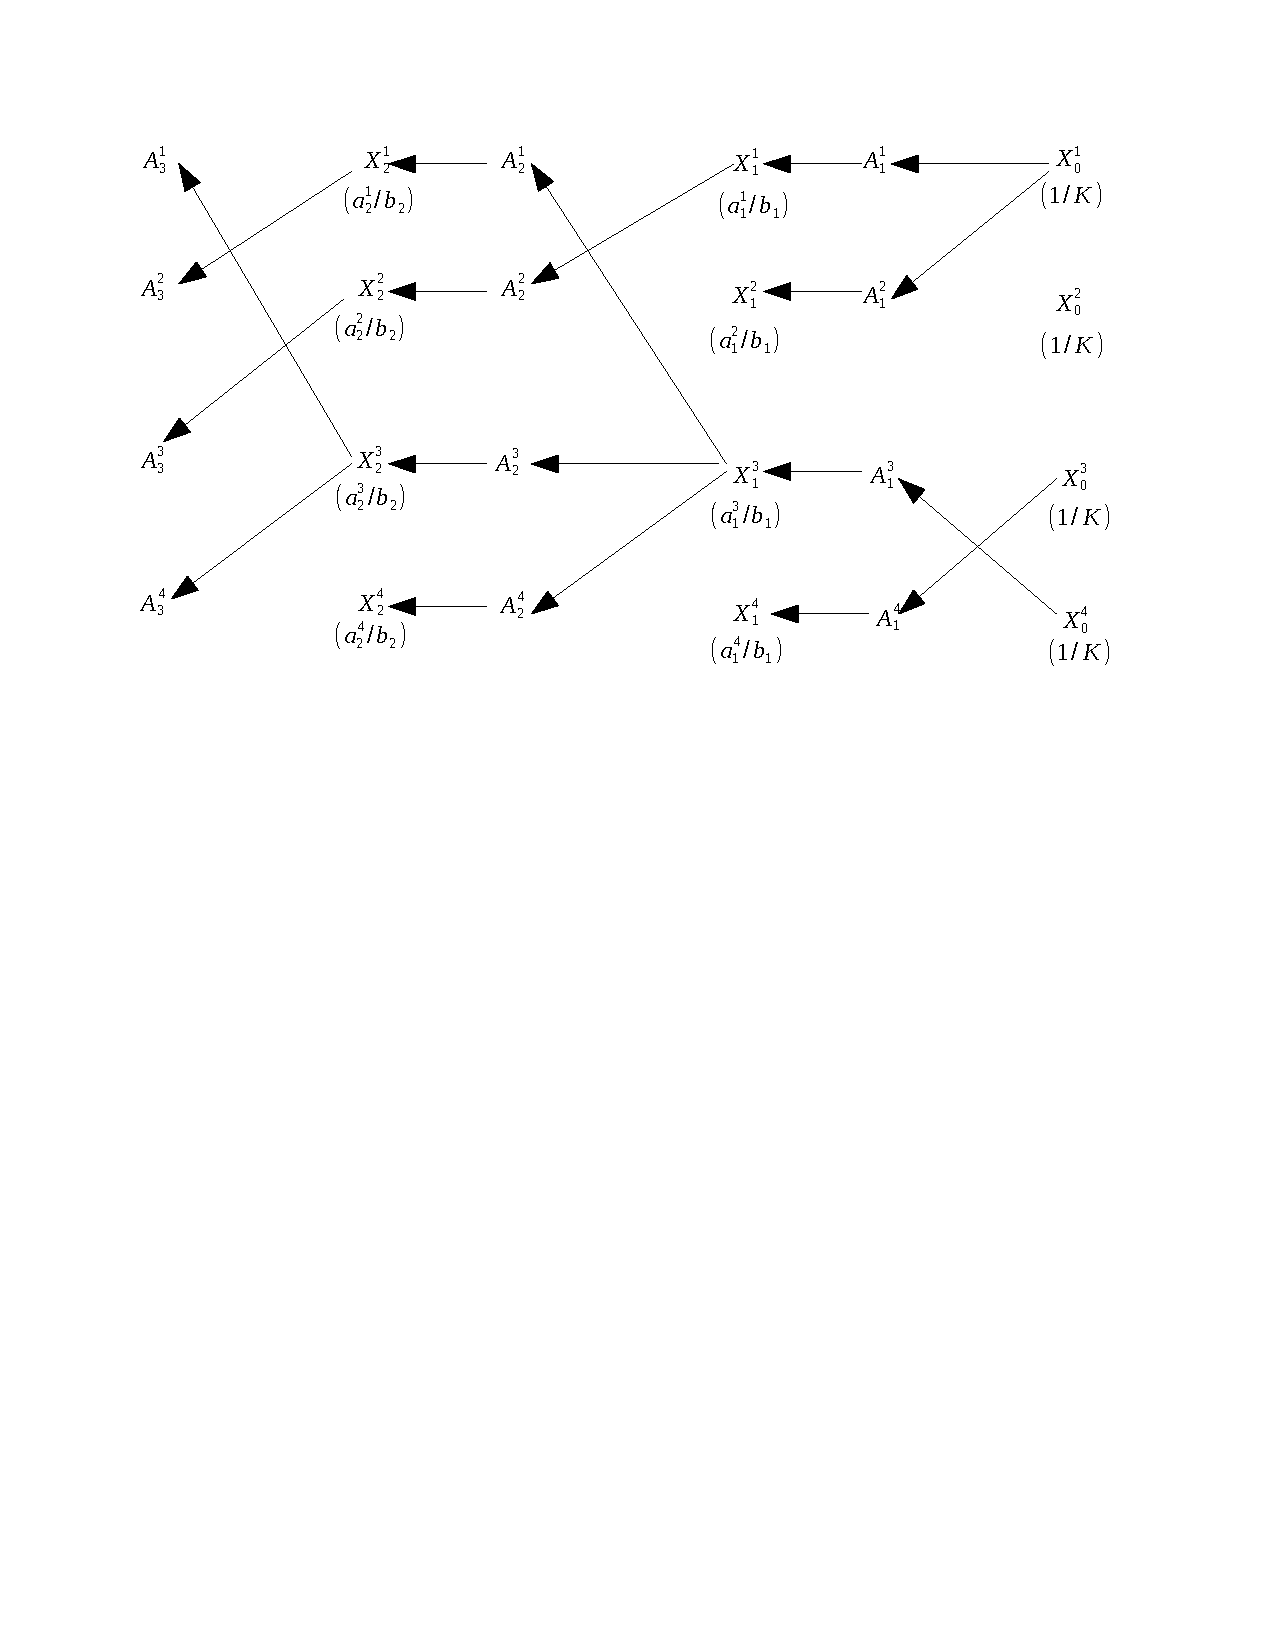
\includegraphics[width=\linewidth, trim=2cm 16cm 2.5cm 2cm, clip]{AnandsEstimator.pdf}
  \caption{A possible realization of the re-sampling procedure. $n =
    3$, $K = 4$. A number in a parenthesis indicates the probability
    of the unit vector above it being chosen to the next step.}
  \label{fig:AnandsEstimator}
\end{figure}
The difficulty with brute-force simulation and estimation is that,
when $n$ is large, the variance of $|\Pi_{n, 1} X_0|^\alpha$
is very large too, resulting in uselessly inaccurate estimations. One
approach of variance reduction is re-sampling. We divide the
estimation of $\Lambda(\alpha)$ into $n$ steps and we are prepared to
simulate $K$ realizations of $A_n, \dots, A_1$ and $X_0$. For
convenience, let
\begin{eqnarray*}
  M_n &=& \Pi_{n, 1} X_0 \\
  X_n &=& {M_n \over |M_n|}
\end{eqnarray*}
We can write
\begin{eqnarray*}
  M_n &=& A_n X_{n - 1} |M_{n - 1}| \\
  &=& A_n X_{n - 1} |A_{n-1} X_{n-2}| \cdot |M_{n-2}| \\
  &=& \cdots \\
  |M_n|^\alpha &=& \prod_{i=1}^n |A_i X_{i-1}|^\alpha
\end{eqnarray*}
With $K$ realizations of $A_n, \dots, A_1$ and $X_0$, a brute-force
estimator of ${1 \over n} \log(\E |M_n|^\alpha)$ can be
\[
{1 \over n} \log \left(
  {1 \over K} \sum_{l=1}^K \prod_{i=1}^n |A_i^l X^l_{i-1}|^\alpha
\right)
\]
where $A_i^l$ denotes the $l$-th realization of $A_i$ and
$X^l_{i-1} = A_{i-1}^l X^l_{i-2}/|A_{i-1}^l X^l_{i-2}|$. To reduce the
variance of the estimator, we introduce a re-sampling procedure:
\begin{equation}
  \label{eq:AnandsEstimator}
  \mathscr E_\alpha =
  {1 \over n}
  \sum_{i=1}^n \log \left(
    {1 \over K}\sum_{l=1}^K |A_i^l X^{w_{l, i-1}}_{i-1}|^\alpha
  \right)
\end{equation}
where the random variable $w_{l, i-1}$ has conditional distribution
\begin{eqnarray*}
  \P(w_{l, i-1} = j | w_{1, i-2}, \dots, w_{K, i-2}) &=& {a^j_{i-1} \over b_{i-1}} \\
  a_{i-1}^j &=& |A_{i-1}^j X_{i-2}^{w_{j, i-2}}|^\alpha \\
  b_{i-1} &=& \sum_{l=1}^K a_{i-1}^l
\end{eqnarray*}
\begin{theorem}
  \[
  \E \left\{
    \sum_{i=1}^n \log \left(
      {1 \over K}\sum_{l=1}^K |A_i^l X^{w_{l, i-1}}_{i-1}|^\alpha
    \right)
  \right\} = \log \left(
    \E |\Pi_{n, 1} X_0|^\alpha
  \right)
  \]
\end{theorem}
Figure \ref{fig:AnandsEstimator} shows a possible realization of the
resampling procedure and algorithm \ref{alg:Lambda_estimation}
outlines an implementation of $\mathscr E_\alpha$. We take
$|\cdot|$ as the max norm.
For an GARCH($p, q$) processes, the $A_i$ matrices have dimension
$d \times d$, where $d = p + q - 1$, and the $X_i$ are $d$-dimensional
unit vectors. 
\begin{algorithm}[H]
  \caption{Algorithm for estimating
    $\Lambda(\alpha) = \lim_{n \to \infty} {1 \over n} \log\left(\E |\Pi_{n, 1}|^\alpha \right)$}
  \label{alg:Lambda_estimation}
  \begin{algorithmic}
    \Procedure{$\mathscr E_\alpha$}{$n, K$}
    \State Define $K$ $d$-dimensional vectors $X^1, \dots, X^K$
    \State Define $K$ $d$-dimensional vectors $Y^1, \dots, Y^K$
    \State Define $K$-dimensional vector $a \gets (1, 1, \dots, 1)$
    \Comment{Initialize the weights}
    \For {$i$ from 1 to $K$}\Comment{Generate initial unit vectors}
    \For {$k$ from 1 to $d$}
    \State Generate a $U(0, 1)$ variable $U$
    \State $X^i(k) \gets U$ \Comment{$X^i(k)$ is the $k$-th component of $X^i$}
    \EndFor
    \State $X^i \gets X^i/|X^i|$
    \EndFor

    $\Lambda \gets 0$

    \For{$j$ from 1 to $n$}

    \State Define $K$-dimensional vector $Q$
    \State $Q(k) \gets \sum_{i=1}^k a(i)$ for all $k=1,2,\dots, K$
    \State Generate $K$ $d \times d$ random matrices $A^1, \dots, A^K$.

    \For{$k$ from 1 to $K$}
    \State Generate a $U(0, Q(K))$ variable $U$.
    \State $l \gets \min\{1 \leq i \leq K: Q(i) > U\}$
    \State $Y^k \gets A^k X^l$
    \State $a(k) \gets |Y^k|$
    \State $Y^k \gets Y^k/a(k)$
    \State $a(k) \gets a(k)^\alpha$
    \EndFor

    \State For all $k=1,\dots,K$, $X^k \gets Y^k$
    \State $\Lambda \gets \Lambda + {1 \over n}\log\left( { Q(K) \over K} \right)$
    \EndFor
    \State $\Lambda \gets \Lambda + {1 \over n}\log\left[ {1 \over K}\sum_{k=1}^K a(k) \right]$

    \Return $\Lambda$
    \EndProcedure
  \end{algorithmic}
\end{algorithm}

%% \ifestimation
\section{Sampling from the shifted conditional distribution}
While the Radon-Nikodym derivative of the shifted conditional
probability measure with respect to the original measure is given by
\eqref{eq:sampling}, the procedure of sampling from the shifted
conditional distribution is not trivial. For this purpose, we first
sample from the original distribution, and obtain an iid sample
$\hat Z_1^2, \hat Z_2^2, \dots, \hat Z_n^2$. This allows us to
compute, empirically, the shifted conditional distribution function
and its inverse:
\begin{eqnarray*}
  F_\xi(a, x) =
  \P^\xi(Z_t^2 \leq a | X_{t-1} = x) 
  &=&
  \int_0^a {
    |A(w)|^\xi r_\xi(A(w) \cdot x)
    \over
    r_\xi(x)
  } f_{Z^2}(w) dw \\
  \hat F_\xi(a, x)
  &=&
  \sum_{i=1}^n {
    |A(\hat Z_i^2)|^\xi r_\xi(A(\hat Z_i^2) \cdot x)
    \over
    r_\xi(x)
  } \1{\hat Z_i^2 \leq a } f_{Z^2}(\hat Z_i^2)
\end{eqnarray*}
where $f_{Z^2}$ denotes the original distribution of
$Z^2 \sim Z_i^2, i=1,2,\dots$ and  $\hat F_\xi(a, x)$ denotes the
empirical conditional distribution function. Now that $\hat F_\xi(a,
x)$ can be computed, one can also compute $\hat F_\xi^{-1}(p, x)$. Let
\[
k = \left\{
  \begin{array}{ll}
    \max\{1 \leq i \leq n: F_\xi(\hat Z_{(i)}^2, x) \leq p\} &
    \hat F_\xi(\hat Z_{(1)}, x) \leq p \\
    0 & \text{ otherwise }
  \end{array}
\right.
\]
where $\hat Z_{(1)}^2 < \cdots < \hat Z_{(i-1)}^2 < \hat Z_{(i)}^2 < \cdots <
\hat Z_{(n)}^2$ denote the order statistics of the sample $\{\hat
Z_{i}^2\}_{i=1}^n$. Then we assign
\[
\hat F_\xi^{-1}(p, x)
= \left\{
  \begin{array}{ll}
    \hat Z_{(1)}^2 + \left[p - \hat F_\xi(\hat Z_{(1)}^2, x)\right] {
      \hat Z_{(2)}^2 - \hat Z_{(1)}^2
      \over
      \hat F_\xi(\hat Z_{(2)}^2, x) - \hat F_\xi(\hat Z_{(1)}^2, x)
    } & k = 0 \\
    \hat Z_{(k)}^2 + \left[p - \hat F_\xi(\hat Z_{(k)}^2, x)\right] \cdot {
      \hat Z_{(k+1)} - \hat Z_{(k)}
      \over
      \hat F_\xi(Z_{(k+1)}, x) - \hat F_\xi(Z_{(k)}, x)
    } & 1 \leq k < n \\
    \hat Z_{(n)}^2 + \left[p - \hat F_\xi(\hat Z_{(n)}^2, x)\right] {
      \hat Z_{(n)}^2 - \hat Z_{(n-1)}^2
      \over
      \hat F_\xi(\hat Z_{(n)}^2, x) - F_\xi(\hat Z_{(n-1)}^2, x)
    } & k = n
  \end{array}
\right.
\]
In plain words, if $\hat F_\xi(\hat Z_{(1)}^2, x) < p < \hat F_\xi(\hat
Z_{(n)}^2, x)$, we interpolate the empirical quantile function; if
$p < \hat F_\xi(\hat Z_{(1)}^2, x)$, we compute $\hat F_\xi^{-1}(p,
x)$ by approximating the probability density function between
$\hat F_\xi^{-1}(p, x)$ and $\hat Z_{(1)}^2$ with ${\hat Z_{(2)}^2 - \hat
  Z_{(1)}^2 \over \hat F_\xi(\hat Z_{(2)}^2, x) - \hat F_\xi(\hat
  Z_{(1)}^2, x)}$; if $p > \hat F_\xi(\hat Z_{(n)}^2, x)$, $\hat F_\xi^{-1}(p,
x)$ is similarly approximated as in the previous case.

With a procedure to compute $\hat F^{-1}_\xi(p, x)$, we can sample
from the conditional distribution $\hat F_\xi(\cdot, x)$ by first
generating a $U(0, 1)$ random variable $U$ and giving
$\hat F^{-1}_\xi(U, x)$ as the desired random variable.

\section{An example: The GARCH(2,1) process}
As an example of the algorithms described in the previous sections, we
consider GARCH(2,1) processes. In this particular case we have
\begin{eqnarray*}
  \sigma_t^2 &=& \omega + \alpha_1 R_{t-1}^2 + \alpha_2 R_{t-2}^2 +
  \beta_1 \sigma_{t-1}^2
\end{eqnarray*}
Or in matrix forms
\begin{eqnarray}
  \begin{pmatrix}
    \sigma_t^2 \\
    R_{t-1}^2
  \end{pmatrix}
  &=&
  \begin{pmatrix}
  \alpha_1 Z_{t-1}^2 + \beta_1 & \alpha_2 \\
  Z_{t-1}^2 & 0
  \end{pmatrix}
  \begin{pmatrix}
    \sigma_{t-1}^2 \\
    R_{t-2}^2
  \end{pmatrix}
  +
  \begin{pmatrix}
    \omega \\
    0
  \end{pmatrix}
  \label{eq:garch21} \\
  V_t &=& A_t V_{t-1} + B \nonumber
\end{eqnarray}
where $R_t$ is the $t$-th observation of the sequence in question and
$Z_t$ are i.i.d $N(0,1)$ random variables. In the following we check
the conditions of theorem \ref{thrm:efficiency} against this process. 

As mentioned in remark \ref{remark:fhrtgh}, Bollerslev's assumption
$\alpha_1 + \alpha_2 + \beta_1 < 1$ implies that the top Lyapunov
exponent associated with the model \eqref{eq:garch21} is
negative. In the following we check the condition of theorem
\ref{thrm:efficiency} with regard to this model.

\begin{lemma}
  \label{lemma:frth}
  Assume $Z_t$ are i.i.d $N(0,1)$ random variables. Then
  $b^{1 - \xi/s} < e^\gamma$, where $b$ is defined in lemma
  \ref{lemma:2}, $\xi$ is the tail index of the stationary
  distribution of the markov chain $V_t$ as defined by
  \eqref{eq:garch21} and $\gamma$ is the top Lyapunov
  exponent of the matrices $A_t$ in \eqref{eq:garch21}.
\end{lemma}
\begin{proof}
First of all, we note $s$ of condition (I), hypothesis \ref{hypo:1}
can be arbitrarily large since $Z_t$ are i.i.d $N(0,1)$ random
variables. Therefore $b^{1 - \xi/s} < e^\gamma$ holds if $b <
e^\gamma$. To show the latter inequality holds, it suffices to show
there exists $\theta \in (0, \xi)$ such that $b_\theta < e^\gamma$,
where $b_\theta$ is defined in lemma \ref{lemma:1}.

If $\theta < 1$, $b_\theta$ is given by \eqref{eq:kpofew}:
\[
b_\theta = 
\lambda(\theta)
\left[
  1 + 
  {|B|^\theta r_{\theta}(\tilde B) 
    \over
    \lambda(\theta) M_{\theta} \underline r_\theta
  }
  \right]
\]
Because $M_\theta$ can be chosen arbitrarily large,
$b_\theta < e^\gamma$ holds if $\lambda(\theta) < e^\gamma$, or
equivalently $\log(\lambda(\theta)) < \gamma$.
Applying theorem 2 of Hennion \cite{hennion:1997} gives, for
an arbitrary fixed $\epsilon > 0$, there exists $N > T$ such that for
all $n > N$, ${1 \over n} \log \|\Pi_{n,1}\| < \gamma + \epsilon$.
This implies
\begin{equation*}
  {1 \over n} \log\left(
  \E \|\Pi_{n,1} \|^\theta
  \right)
  <
  \theta (\gamma + \epsilon)
  \]
  Thus
  \[
  \log(\lambda(\theta))
  =
  \lim_{n \to \infty} {1 \over n} \log\left(
  \E \|\Pi_{n,1} \|^\theta
  \right)
  <
  \theta (\gamma + \epsilon)
\end{equation*}
Thus, if $\theta$ is chosen such that
$0 < \theta < {\gamma \over \gamma + \epsilon} < 1$,
we have $b_\theta < e^\gamma$. The proof is complete.
\end{proof}

\subsection{Evaluation of the right eigenfunction}
Recall that, for $0 < \theta < \xi$, the right eigenfunction
$r_\theta(\cdot)$ corresponding to eigenvalue $\lambda(\theta)$ of the
operator $\mathscr P^\theta$ defined in \eqref{eq:trhyh} satisfies
\begin{eqnarray}
  \label{eq:trhj}
  \E \left[
    |A x|^\theta r_\theta(A \cdotp x)
    \right]
  &=&
  \mathscr P^\theta r_\theta(x) = \lambda(\theta) r_\theta(x)
\end{eqnarray}
In the following we take $|\cdot|$ as the Euclidean norm. Then $x$
can be written as $x = (\cos w, \sin w)^\top$, $w \in (0, \pi/2)$ and
\begin{eqnarray*}
  A x &=&
  \begin{pmatrix}
    \alpha_2 \sin w + (Z_t^2 \alpha_1 + \beta_1) \cos w \\
    Z^2 \cos w
  \end{pmatrix}
\end{eqnarray*}
Let $A \cdot x = (\cos \varphi, \sin\varphi)^\top$. Then
\begin{eqnarray}
  Z_t^2 &=&
  {\tan\varphi (\alpha_2 \sin w + \beta_1 \cos w)
    \over
    \cos w (1- \alpha_1 \tan\varphi)
  } \label{eq:rthy} \\
  {d Z_{t}^2 \over d\varphi}
  &=&
  {
    (\alpha_2 \sin w + \beta_1 \cos w) \sec^2\varphi
    \over
    \cos w (1 - \alpha_1 \tan\varphi)^2
  } \nonumber
\end{eqnarray}
Using \eqref{eq:rthy} we can write
\[
|A x|^{\theta}
=
(\alpha_2^2 + \beta_1^2)^{\theta/2}
{
  \sin^\theta\left(
  w + \arctan{\beta_1 \over \alpha_2}
  \right)
  \over
  \cos^\theta\varphi (1 - \alpha_1 \tan\varphi)^\theta
}
\]
It also becomes clear from \eqref{eq:rthy}
\[
x \in \left\{(\cos w, \sin w)^\top:
w \in \Omega = \left[0, \arctan{1 \over \alpha_1}\right)
\right\}
\quad
t = 0,1,2,\dots
\]
Define
\[
h_\theta(w): w \in \Omega \to (\underline r_\theta, \bar r_\theta)
\ni r_\theta((\cos w, \sin w)^\top)
\]
Then \eqref{eq:trhj} can be rewritten as
\begin{eqnarray}
  \lambda(\theta) h_\theta(w)
  &=&
\int_\Omega (\alpha_2^2 + \beta_1^2)^{\theta/2} {
  \sin^\theta\left(
  w + \arctan{\beta_1 \over \alpha_2}
  \right)
  \over
  \cos^\theta\varphi (1 - \alpha_1 \tan\varphi)^\theta
}
f_{\chi^2}\left[
{\tan\varphi (\alpha_2 \sin w + \beta_1 \cos w)
  \over
  \cos w (1- \alpha_1 \tan\varphi)
} \right] \times \nonumber\\
&&
h_\theta(\varphi)
{
  (\alpha_2 \sin w + \beta_1 \cos w) \sec^2\varphi
  \over
  \cos w (1 - \alpha_1 \tan\varphi)^2
}
d\varphi \nonumber \\
\lambda(\theta) h_\theta(w)
&=&
\int_\Omega H_\theta(w, \varphi) h_\theta(\varphi) d\varphi
\end{eqnarray}
where $f_{\chi^2}(\cdot)$ is the probability density function of the
$\chi^2$ distribution; the function $H_\theta(w, \varphi)$ has been defined
for convenience.
We may approximate the last integral with a sum and the function
$h_\theta(\cdot)$ with a vector:
\[
\lambda(\theta) h_\theta(i \Delta_n)
\approx
\Delta_n \sum_{j=0}^{n-1} H_\theta(i \Delta_n, j \Delta_n) h_\theta(j \Delta_n)
\]
where $\Delta_n = {\arctan(1/\alpha_1) \over n}$.
Thus $\lambda(\theta)$ can be found as the spectral radius of 
matrix $\Delta_n H_\theta(i \Delta_n, j \Delta_n)$ and 
$\{h_\theta(i \Delta_n)\}_ {i=1,2,\dots, n}$ as the associated
eigenvector (cf. Collamore and Mentemeier
\cite{collamore:mentemeier:2016}, lemma 2.2).

\subsection{Simulaton and Results}
In this section we describe the implementation of the estimator
$\mathcal E_u$ when $V_t$ is a GARCH($2, 1$) process. In previous
sections we have shown that $\mathcal E_u$ is efficient for
GARCH($2, 1$) and described how the right eigenfunctions can be
approximately evaluated. It remains to choose the set
$\mathcal C = \{v \in \chi, |V_n| < M\}$.

For convenience, we take $\Theta = [\xi/4, 3\xi/4]$
(cf. \S\ref{sec:bound_to_C}).


% To estimate the 
% values of $\omega, \alpha_1, \alpha_2, \beta_1$, we use the ``fGarch''
% package of the ``R'' language. Its ``garchFit'' function provides
% routine to fit a specified type of model to a given series.
% The ``garchFit'' function provides 4 algorithms for maximum likelihood
% estimation of the parameters. We choose its default algorithm ``nlminb'',
% i.e. ``unconstrained and box-constrained optimization using PORT
% routines''. The ``fGarch'' package is developed and maintained by {\it
% Rmetrics} (https://www.rmetrics.org/).

  
% \subsubsection{S\&P 500}
% \begin{itemize}
% \item GARCH(1, 1)
%   When modeled as a GARCH(1, 1) process, the S\&P 500 return series
%   has the coefficients as shown in the following equation
%   \[
%   \sigma_t^2 = 0.15 R_{t-1}^2 + 0.72 \sigma_{t-1}^2 + 7.4 \times 10^{-6}
%   \]
%   The tail index of the stationary distribution of $\sigma_t^2$ is
%   estimated at 4.4465. On the other hand, the Hill estimator puts the
%   tail index of the inferred $\sigma_t^2$ at 4.3372.

% \item GARCH(2, 1)
%   When fitted to a GARCH(2, 1) process, the S\&P 500 return series has
%   the following model
%   %% 7.949678e-02, 8.765884e-02, 9.376992e-06
%   \[
%   \sigma_t^2 = 0.079 R_{t-1}^2 + 0.088 R_{t-2}^2 + 0.668 \sigma_{t-1}^2 + 9.4 \times 10^{-6}
%   \]
%   Using the proposed re-sampling algorithm, our estimate of the tail
%   index is $4.30026$. The values of $\Lambda(\alpha)$ in the
%   neighborhood of $\alpha = \xi$ is listed in table
%   \ref{tab:SP500_garch21_tail_index}.
%   \begin{table}[htb!]
%     \centering
%     \begin{tabular}{l|l|l|l||l|l|l|l}
%       $\alpha$ & $\Lambda(\alpha)$ & err. & rel. err. & $\alpha$ & $\Lambda(\alpha)$ & err. & rel. err. \\
%       \hline
%       0.1000 & -0.0186 & 0.0007 & 0.0378 & 3.1000 & -0.2020 & 0.2175 & 1.0766\\
%       0.2000 & -0.0366 & 0.0012 & 0.0329 & 3.2000 & -0.1921 & 0.2360 & 1.2286\\
%       0.3000 & -0.0539 & 0.0016 & 0.0293 & 3.3000 & -0.1829 & 0.2765 & 1.5116\\
%       0.4000 & -0.0706 & 0.0020 & 0.0281 & 3.4000 & -0.1705 & 0.3121 & 1.8308\\
%       0.5000 & -0.0866 & 0.0024 & 0.0279 & 3.5000 & -0.1595 & 0.3335 & 2.0914\\
%       0.6000 & -0.1018 & 0.0030 & 0.0299 & 3.6000 & -0.1458 & 0.3665 & 2.5140\\
%       0.7000 & -0.1163 & 0.0045 & 0.0387 & 3.7000 & -0.1264 & 0.4249 & 3.3627\\
%       0.8000 & -0.1301 & 0.0059 & 0.0456 & 3.8000 & -0.1165 & 0.4285 & 3.6778\\
%       0.9000 & -0.1432 & 0.0083 & 0.0581 & 3.9000 & -0.0996 & 0.5233 & 5.2545\\
%       1.0000 & -0.1552 & 0.0104 & 0.0668 & 4.0000 & -0.0819 & 0.5479 & 6.6896\\
%       1.1000 & -0.1666 & 0.0137 & 0.0825 & 4.1000 & -0.0653 & 0.5806 & 8.8930\\
%       1.2000 & -0.1771 & 0.0168 & 0.0947 & 4.2000 & -0.0403 & 0.7173 & 17.8196\\
%       1.3000 & -0.1867 & 0.0206 & 0.1105 & 4.3000 & -0.0365 & 0.6749 & 18.5091\\
%       1.4000 & -0.1958 & 0.0246 & 0.1255 & 4.4000 & -0.0055 & 0.7390 & 135.2172\\
%       1.5000 & -0.2038 & 0.0299 & 0.1467 & 4.5000 & 0.0186 & 0.8443 & 45.4573\\
%       1.6000 & -0.2107 & 0.0353 & 0.1675 & 4.6000 & 0.0267 & 0.7493 & 28.0286\\
%       1.7000 & -0.2169 & 0.0398 & 0.1836 & 4.7000 & 0.0614 & 0.9068 & 14.7576\\
%       1.8000 & -0.2226 & 0.0467 & 0.2099 & 4.8000 & 0.0867 & 0.9380 & 10.8220\\
%       1.9000 & -0.2271 & 0.0543 & 0.2392 & 4.9000 & 0.0973 & 0.8703 & 8.9467\\
%       2.0000 & -0.2299 & 0.0607 & 0.2642 & 5.0000 & 0.1275 & 0.9424 & 7.3918\\
%       2.1000 & -0.2320 & 0.0685 & 0.2953 & 5.1000 & 0.1618 & 1.0582 & 6.5403\\
%       2.2000 & -0.2344 & 0.0760 & 0.3244 & 5.2000 & 0.1721 & 0.8950 & 5.2004\\
%       2.3000 & -0.2343 & 0.0903 & 0.3856 & 5.3000 & 0.2081 & 0.9849 & 4.7334\\
%       2.4000 & -0.2341 & 0.0994 & 0.4246 & 5.4000 & 0.2411 & 1.0852 & 4.5009\\
%       2.5000 & -0.2320 & 0.1106 & 0.4767 & 5.5000 & 0.2378 & 0.9362 & 3.9375\\
%       2.6000 & -0.2291 & 0.1273 & 0.5555 & 5.6000 & 0.2605 & 0.9805 & 3.7635\\
%       2.7000 & -0.2273 & 0.1365 & 0.6007 & 5.7000 & 0.3306 & 1.0445 & 3.1596\\
%       2.8000 & -0.2214 & 0.1595 & 0.7205 & 5.8000 & 0.3301 & 1.0014 & 3.0333\\
%       2.9000 & -0.2143 & 0.1667 & 0.7781 & 5.9000 & 0.3562 & 1.0427 & 2.9270\\
%       3.0000 & -0.2075 & 0.2034 & 0.9804 & 6.0000 & 0.3891 & 0.9544 & 2.4525
%     \end{tabular}
%     \caption{SP500: $\Lambda(\alpha)$ around $\alpha = \xi$. N = 400, K = 40000}
%     \label{tab:SP500_garch21_tail_index}
%   \end{table}

%   \begin{minipage}{0.5\linewidth}
%     \centering
%     $\Lambda(\alpha)$
%     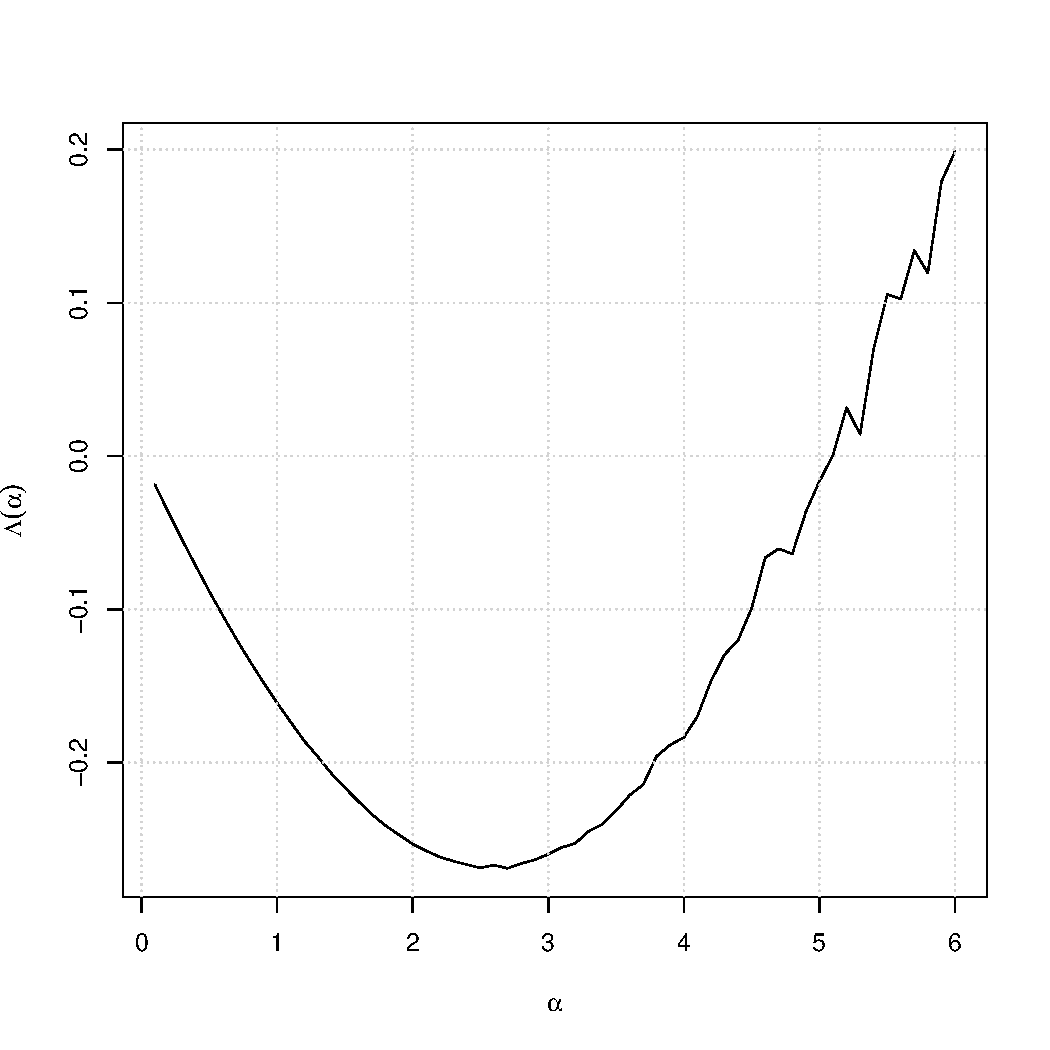
\includegraphics[width=\textwidth]{SP500_xi.pdf}
%   \end{minipage}\hfill
%   \begin{minipage}{0.5\linewidth}
%     \centering
%     $r_\xi(x)$ corresponding to $\xi$
%     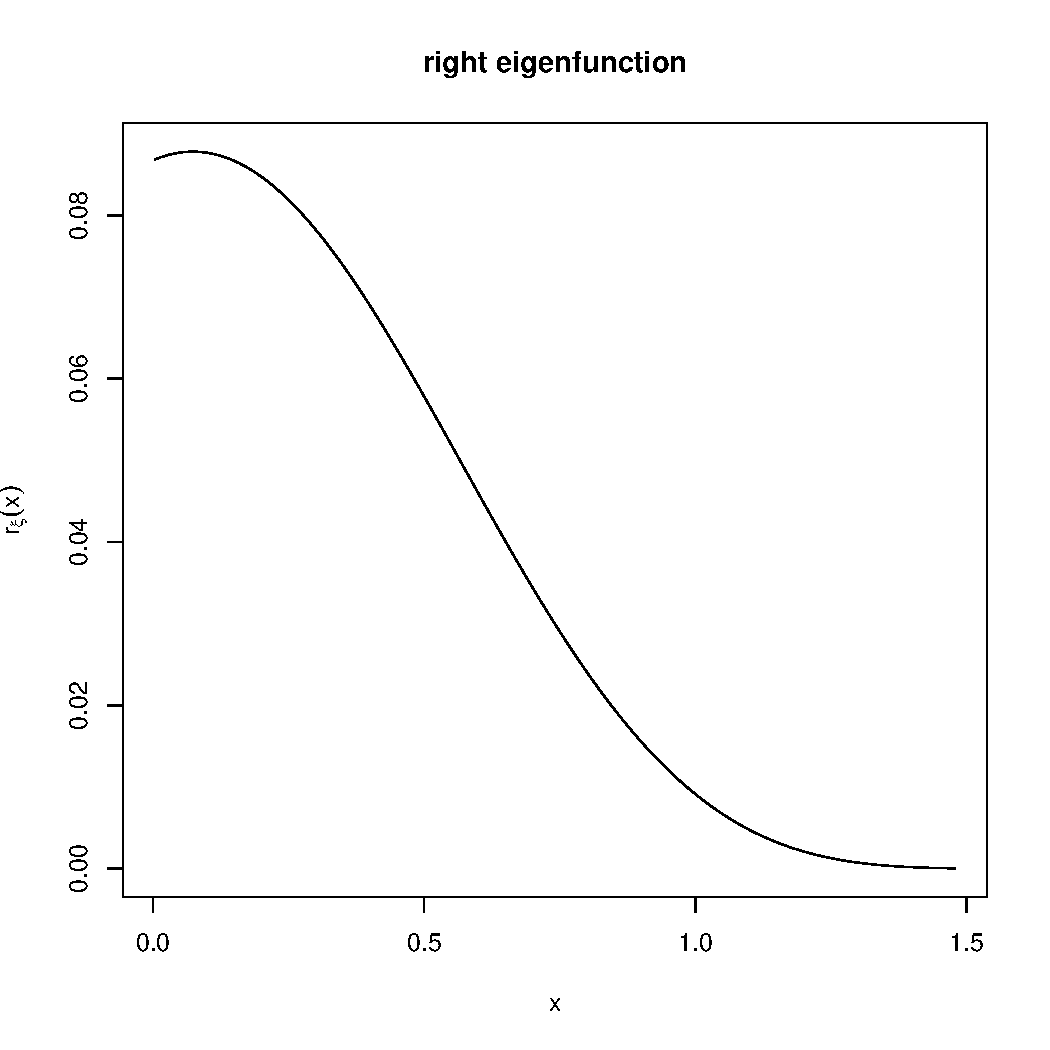
\includegraphics[width=\textwidth]{SP500_r.pdf}
%   \end{minipage}
% \end{itemize}

% \subsubsection{DAX}
% \begin{itemize}
% \item GARCH(1, 1)
%   When modeled as a GARCH(1, 1) process, the DAX return series
%   has the coefficients as shown in the following equation
%   \[
%   \sigma_t^2 = 0.06 R_{t-1}^2 + 0.92 \sigma_{t-1}^2 + 3.1 \times 10^{-6}
%   \]
%   The tail index of the stationary distribution of $\sigma_t^2$ is
%   estimated at 6.4269. The Hill estimator of this
%   sequence is computed at 6.6020.

% \item GARCH(2, 1)
%   When fitted to a GARCH(2, 1) process, the DAX return series has the following model
%   \[
%   \sigma_t^2 = 0.027 R_{t-1}^2 + 0.042 R_{t-2}^2 + 0.897 \sigma_{t-1}^2 + 4.0 \times 10^{-6}
%   \]
%   The algorithm with its current implementation has difficulty to
%   estimate $\Lambda(\alpha)$ as $\alpha$ becomes large. This is shown
%   in the figure below:
%   \begin{figure}[htb!]
%     \centering
%     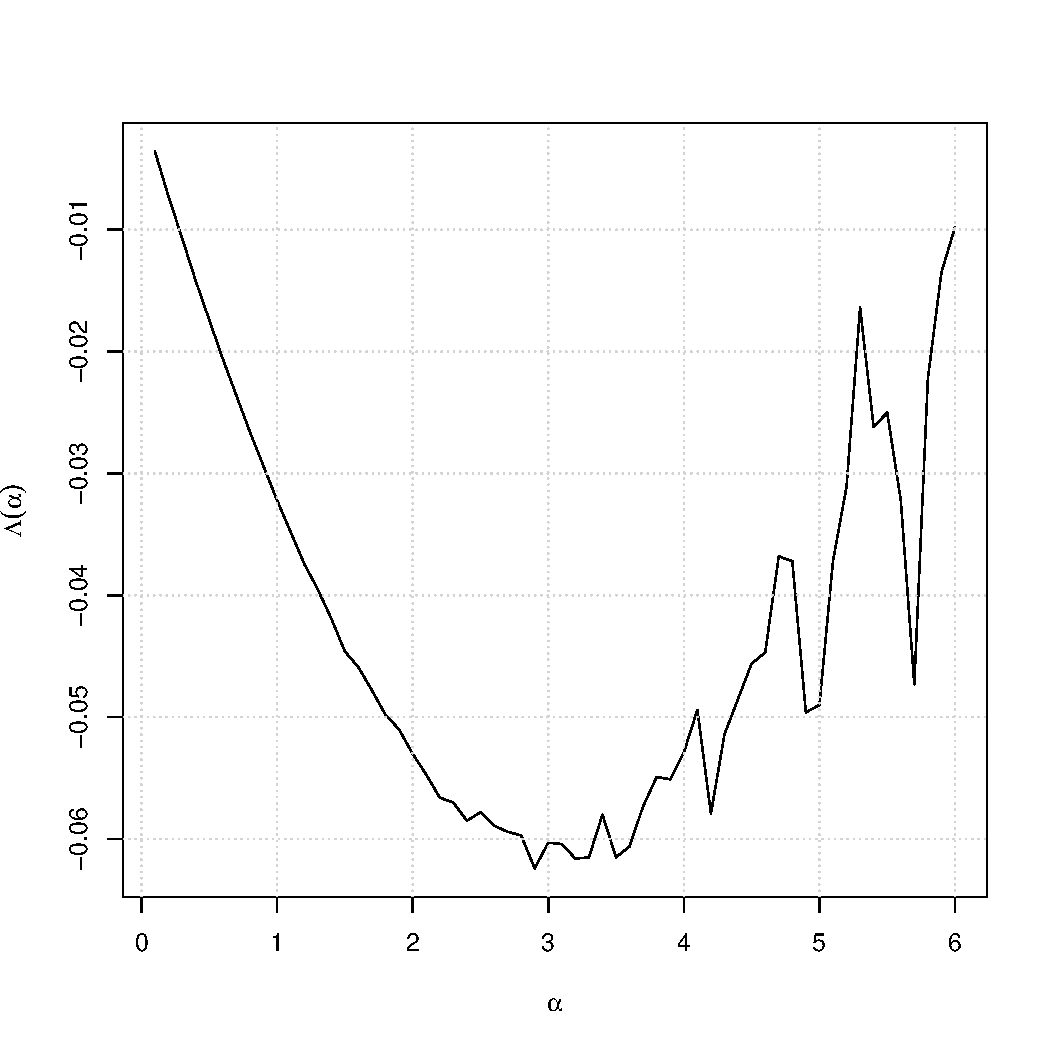
\includegraphics[width=\textwidth]{DAX_xi.pdf}
%     \caption{$\Lambda(\alpha)$ estimates for DAX}
%     \label{fig:DAX_garch21_tailindex}
%   \end{figure}
%   The estimated values of $\Lambda(\alpha)$ are listed table \ref{tab:DAX_garch21_tail_index}.
%     \begin{table}[htb!]
%     \centering
%     \begin{tabular}{l|l|l|l||l|l|l|l}
%       $\alpha$ & $\Lambda(\alpha)$ & err. & rel. err. & $\alpha$ & $\Lambda(\alpha)$ & err. & rel. err. \\
%       \hline
%       0.1000 & -0.0036 & 0.0009 & 0.2535 & 3.1000 & -0.0604 & 0.2027 & 3.3558 \\
%       0.2000 & -0.0073 & 0.0017 & 0.2340 & 3.2000 & -0.0616 & 0.2585 & 4.1940 \\
%       0.3000 & -0.0107 & 0.0020 & 0.1903 & 3.3000 & -0.0615 & 0.2669 & 4.3419 \\
%       0.4000 & -0.0142 & 0.0025 & 0.1763 & 3.4000 & -0.0580 & 0.3232 & 5.5729 \\
%       0.5000 & -0.0174 & 0.0027 & 0.1531 & 3.5000 & -0.0615 & 0.3719 & 6.0467 \\
%       0.6000 & -0.0206 & 0.0030 & 0.1445 & 3.6000 & -0.0606 & 0.3794 & 6.2604 \\
%       0.7000 & -0.0236 & 0.0038 & 0.1624 & 3.7000 & -0.0573 & 0.4485 & 7.8213 \\
%       0.8000 & -0.0266 & 0.0050 & 0.1884 & 3.8000 & -0.0549 & 0.5345 & 9.7438 \\
%       0.9000 & -0.0294 & 0.0073 & 0.2469 & 3.9000 & -0.0551 & 0.5655 & 10.2685 \\
%       1.0000 & -0.0322 & 0.0089 & 0.2774 & 4.0000 & -0.0529 & 0.6865 & 12.9826 \\
%       1.1000 & -0.0348 & 0.0109 & 0.3127 & 4.1000 & -0.0494 & 0.7077 & 14.3304 \\
%       1.2000 & -0.0374 & 0.0146 & 0.3904 & 4.2000 & -0.0579 & 0.7418 & 12.8088 \\
%       1.3000 & -0.0395 & 0.0178 & 0.4515 & 4.3000 & -0.0514 & 0.8021 & 15.6075 \\
%       1.4000 & -0.0419 & 0.0218 & 0.5210 & 4.4000 & -0.0485 & 0.9369 & 19.3079 \\
%       1.5000 & -0.0446 & 0.0260 & 0.5821 & 4.5000 & -0.0456 & 0.9525 & 20.8980 \\
%       1.6000 & -0.0459 & 0.0304 & 0.6634 & 4.6000 & -0.0447 & 1.0402 & 23.2610 \\
%       1.7000 & -0.0478 & 0.0356 & 0.7443 & 4.7000 & -0.0368 & 1.0678 & 28.9796 \\
%       1.8000 & -0.0498 & 0.0421 & 0.8452 & 4.8000 & -0.0372 & 1.1068 & 29.7502 \\
%       1.9000 & -0.0510 & 0.0482 & 0.9443 & 4.9000 & -0.0496 & 1.1848 & 23.8698 \\
%       2.0000 & -0.0530 & 0.0543 & 1.0236 & 5.0000 & -0.0490 & 1.1304 & 23.0528 \\
%       2.1000 & -0.0547 & 0.0650 & 1.1877 & 5.1000 & -0.0372 & 1.3674 & 36.7623 \\
%       2.2000 & -0.0566 & 0.0713 & 1.2610 & 5.2000 & -0.0311 & 1.3533 & 43.5658 \\
%       2.3000 & -0.0570 & 0.0820 & 1.4393 & 5.3000 & -0.0164 & 1.3191 & 80.2003 \\
%       2.4000 & -0.0585 & 0.0914 & 1.5631 & 5.4000 & -0.0262 & 1.4752 & 56.2897 \\
%       2.5000 & -0.0578 & 0.1070 & 1.8514 & 5.5000 & -0.0250 & 1.3379 & 53.5797 \\
%       2.6000 & -0.0589 & 0.1163 & 1.9759 & 5.6000 & -0.0322 & 1.4219 & 44.1810 \\
%       2.7000 & -0.0594 & 0.1302 & 2.1913 & 5.7000 & -0.0473 & 1.3915 & 29.4468 \\
%       2.8000 & -0.0597 & 0.1516 & 2.5405 & 5.8000 & -0.0222 & 1.6773 & 75.3996 \\
%       2.9000 & -0.0624 & 0.1663 & 2.6664 & 5.9000 & -0.0135 & 1.4893 & 110.0806 \\
%       3.0000 & -0.0603 & 0.1877 & 3.1148 & 6.0000 & -0.0098 & 1.5522 & 158.6270
%     \end{tabular}
%     \caption{DAX: $\Lambda(\alpha)$ around $\alpha = \xi$. N = 400, K = 40000}
%     \label{tab:DAX_garch21_tail_index}
%   \end{table}

% \end{itemize}





%extremes Chapter
\chapter[Extreme value analysis for the sample autocovariance matrices of heavy-tailed multivariate time series]{{\huge Extreme value analysis for the sample autocovariance matrices of heavy-tailed multivariate time series}}\label{ch:extremes}
\chaptermark{Sample autocovariance matrices}

\begin{center}
\textsc{Richard Davis, Johannes Heiny, \\Thomas Mikosch \& Xiaolei Xie\\
{\em Extremes 19}, 3 (2016), 517--547.}
\end{center}

\begin{abstract}{We  provide some  asymptotic theory for the largest eigenvalues of a sample covariance matrix
of a $p$-dimensional time series where the dimension $p=p_n$ converges to infinity when the sample size $n$ increases.
We give a short overview of the literature on the topic both in the light- and heavy-tailed cases when the data have
finite (infinite) fourth moment, respectively.
Our main focus is on the heavy-tailed case. In this case, one has a theory for the point process of the normalized eigenvalues
of the sample covariance matrix in the iid case but also when rows and columns of the data are linearly dependent.
We provide limit results for the weak convergence of these point processes to Poisson or cluster Poisson processes. Based o
this convergence we can also derive the limit laws of various functionals of the ordered eigenvalues such as the
joint convergence of a finite number of the largest order statistics, the joint limit law of the largest eigenvalue and the trace,
limit laws for successive ratios of ordered eigenvalues,
etc. We also develop some
limit theory for the singular values of the sample autocovariance matrices and their sums of squares. The theory is illustrated
for simulated data and for the components of the S\&P 500 stock index.
\medskip

\noindent {\bf Keywords:} Regular variation, sample covariance matrix, dependent entries,
largest  eigenvalues, trace, point process
  convergence, cluster Poisson limit,
infinite variance stable limit, Fr\'echet distribution.}
\end{abstract}

\newpage
\section[Estimation of the largest eigenvalues]{Estimation of the largest eigenvalues: an overview in the iid case}\label{sec:motivationch3}
\subsection{The light-tailed case}
%In recent years, \asy\ theory for large random matrices has a
%attracted a
%great deal of attention; see for example the monographs
%Bai and Silverstein \cite{bai:silverstein:2010} and Anderson et al.
%\cite{anderson:guionnet:zeitouni:2008}. The literature about {\em
%  heavy-tailed random matrices} is rather sparse. Here and in what
%follows, we call a random matrix {\em heavy-tailed} if its entries have
%\ds s with \regvary\ tails, typically with tail index below 4.
%The eigenvalues of heavy-tailed matrices
%with iid entries and dimension $p\times n$, where $p=p_n\to\infty$ and $p/n\to
%\gamma\in (0,\infty)$, were studied by Soshnikov \cite{soshnikov:2004,
%  soshnikov:2006} and  Auffinger et
%al. \cite{auffinger:arous:peche:2009}. In the latter reference and in
%Belinschi et al. \cite{belinschi:dembo:guionnet:2009},
%the sample covariance matrices of iid heavy-tailed \seq s were also studied.
%Bose et al. \cite{bose:hazra:saha:2009,bose:hazra:saha:2010}
%investigated the spectral norm of circulant-type heavy-tailed matrices
%and Ben Arous and Guionnet \cite{arous:guionnet:2008}
%studied the limits of heavy-tailed random Wigner matrices with
%infinite variance.
One of the exciting new areas of statistics is concerned with analyses of large data sets.
For such data one often studies the dependence structure via covariances and correlations.
In this paper we focus on one aspect: the estimation of the eigenvalues of the covariance matrix of a multivariate  \ts\
when the dimension $p$ of the series increases with the sample size $n$. In particular, we are interested in limit theory for the largest eigenvalues of the sample covariance matrix. This theory is closely related to topics from classical \evt\ such as
maximum domains of attraction with the corresponding normalizing and centering constants for maxima; cf. Embrechts et al.~\cite{embrechts:kluppelberg:mikosch:1997}, Resnick~\cite{resnick:2007,resnick:1987}.
Moreover, \pp\ \con\ with limiting Poisson and cluster Poisson processes enters in a natural way when one describes
the joint \con\ of the largest eigenvalues of the sample covariance matrix. Large deviation techniques find applications,
linking \evt\ with random walk theory and \pp\ \con . The objective of this paper is to illustrate some of the main
developments in random matrix theory for the particular case of the sample covariance matrix of multivariate \ts\ with
independent or dependent entries. We give special emphasis to the heavy-tailed case when \evt\ enters in a rather
straightforward way.
%We do not cover other parts of random matrix theory such as limit theory for the eigen-spectrum of random matrices with
%iid entries or other special types of matrices. Also in this case one can find many parallels with \evt.
\par
Classical multivariate \tsa\ deals with
observations which assume values in a $p$-dimensional space
where $p$ is ``relatively small'' compared to the sample size $n$.  With
the availability of large data sets $p$ can be ``large''
relative to $n$. One of the possible con\seq s is that standard asymptotics (such as the \clt )
break down and may even cause misleading results.
\par
The dependence
structure in multivariate data is often summarized by the covariance matrix which is typically
estimated by its sample analog.  For example, principal component analysis (PCA)
extracts principal component vectors corresponding to the largest
eigenvalues of the sample covariance matrix. The magnitudes of these eigenvalues provide an empirical \ms\ of the importance
of these components.
\par
If $p,n$ are fixed, a column of the $p\times n$ data matrix
\beao
\X =\X_n = \big(X_{it}\big)_{i=1,\ldots,p;t=1,\ldots,n}\,
\eeao
represents an observation of a $p$-dimensional \ts\ model with unknown parameters.
In this section we assume that the real-valued entries $X_{it}$ are iid, unless mentioned otherwise, and we write $X$ for a generic element.
One challenge is to infer information about the parameters
from the eigenvalues $\lambda_1,\ldots,\lambda_p$
of the {\em sample covariance matrix} $\X\X'$. In the notation we suppress the dependence of $(\la_i)$ on $n$ and $p$.
If $p$ and $n$ are finite and the columns of $\X$ are iid and multivariate normal,
Muirhead \cite{muirhead} derived a (rather complicated) formula for the joint distribution of the eigenvalues $(\lambda_i)$.
%Therefore a theoretical solution is already available in the finite $n$ case.
%The expression, however, contains an integral over the orthogonal group $\mathbb{O}(p)$.
%\begin{figure}[htb!]
%  \centering
 % \includegraphics[scale=0.5]{eigen_normal_qqplot1.pdf}
 % \caption{Largest eigenvalues of $500$ simulated sample covariance matrices against standard normal quantiles.}
 % \label{fig:QQ}
%\end{figure}

For $p$ fixed and $\nto$, assuming
$\X$ has centered normal entries and a diagonal covariance matrix $\Sigma$,
Anderson~\cite{anderson:1963}  derived the joint \asy\ density of $(\lambda_1, \ldots, \lambda_p)$.
%If the largest eigenvalue of the underlying covariance matrix appears with multiplicity one, he
%showed that the largest eigenvalue of the sample covariave matrix
%is asymptotically normal.
We quote from Johnstone~\cite{johnstone:2001}:
``The classic paper by Anderson~\cite{anderson:1963} gives the limiting joint distribution of the roots, but the
marginal distribution of the largest eigenvalue is hard to extract even in the null case'' (i.e., when the covariance matrix $\Sigma$ is
proportional to the identity matrix).
%If the largest entry of $\Sigma$ exceeds its second largest, one obtains a central limit type theorem for the largest eigenvalue of the sample covariance matrix.
%In Figure~\ref{fig:QQ} we chose $n=10000, p=50$ and $\Sigma =\diag(1024,1,\ldots,1)$, and plot the properly normalized and
%standardized largest eigenvalue against standard normal quantiles.

It turns out that limit theory for the largest eigenvalues becomes ``easier''
when the dimension $p$ increases with $n$.
Over the last 15 years there has been increasing interest in the case when $p=p_n\to\infty$ as $\nto$. In most of
the literature (exceptions are El Karoui \cite{elkaroui:2003}, Davis et al. \cite{davis:mikosch:pfaffel:2015,davis:pfaffel:stelzer:2014} and Heiny and Mikosch
\cite{heiny:mikosch:2015:iid})
one assumes that $p$ and $n$ grow at the same rate:
\beam\label{eq:gammach3}
\dfrac p n\to \gamma\qquad \mbox{for some $\gamma \in (0,\infty)$.}
\eeam
%One explanation for the commonly used condition \eqref{eq:gamma} is that much of the theory was developed for $n \times n$ {\em Wigner matrices}, which is a Hermitean matrix $H$ such that $\{ H_{ij}:i<j \}$ and $\{ H_{ii}:0\le i\le n \}$ are two sets of iid random variables. If $p =\gamma n$, it turns out that the limit theory for the eigenvalues of Wigner matrices and sample covariance matrices is closely connected by the convergence of the empirical spectral distributions to the semicircle and the Mar\v cenko--Pastur law, respectively; see Bai and Silverstein \cite{bai:silverstein:2010}, Chapters 1-3.

In random matrix theory,  the convergence of the {\em empirical spectral distributions} $(F_{n^{-1}\X \X'})$ of a sequence $(n^{-1}\X \X')$ of non-negative definite matrices is the principle object of study. The empirical spectral distribution $F_{n^{-1}\X \X'}$ is constructed from the eigenvalues via
\begin{equation*}
F_{n^{-1}\X \X'}(x)= \frac{1}{p}\; \# \{ 1\le j\le p : n^{-1} \lambda_j \le x \}, \quad x\in \R,\quad n\ge1.
\end{equation*}
In the literature convergence results for the sequence of empirical spectral distributions are established under the assumption that $p$ and $n$ grow at the same rate.
Suppose that the iid entries $Z_{it}$ have mean $0$ and variance $1$. If \eqref{eq:gammach3} holds, then, with probability one, $(F_{n^{-1}\X \X'})$ converges weakly to the celebrated Mar\v cenko--Pastur law $F_\gamma$. If $\gamma \in (0,1]$,  $F_\gamma$  has density,
\begin{eqnarray}\label{eq:MPch3}
f_\gamma(x) =
\left\{\begin{array}{ll}
\frac{1}{2\pi x\gamma} \sqrt{(b-x)(x-a)} \,, & \mbox{if } a\le x \le b, \\
 0 \,, & \mbox{otherwise,}
\end{array}\right.
\end{eqnarray}\noindent
where $a=(1-\sqrt{\gamma})^2$ and $b=(1+\sqrt{\gamma})^2$. If $\gamma>1$, the \MP law is a mixture of a point mass at $0$ and the density function $f_{1/\gamma}$ with weights $1-1/\gamma$ and $1/\gamma$, respectively.  The point mass at $0$ is intuitively explained by the fact that, with probability $1$, $\min(p,n)$ eigenvalues $\lambda_i$ are non-zero. When $n=(1/\gamma) \; p$ and $\gamma >1$ one sees that the proportion of non-zero eigenvalues of the sample covariance matrix is $1/\gamma$ while the proportion of zero eigenvalues is $1-1/\gamma$.

While the finite second moment is the central assumption to obtain the Mar\v cenko--Pastur law as the limiting spectral distribution, the finite fourth moment plays a crucial role when studying the largest eigenvalues
\beam\label{eq:orderch3}
\la_{(1)}\ge \cdots \ge \la_{(p)}
\eeam
of $\X\X'$, where we suppress the dependence on $n$ in the notation.

\begin{figure}[htb!]
  \centering
  \subfigure[Standard normal entries]{
    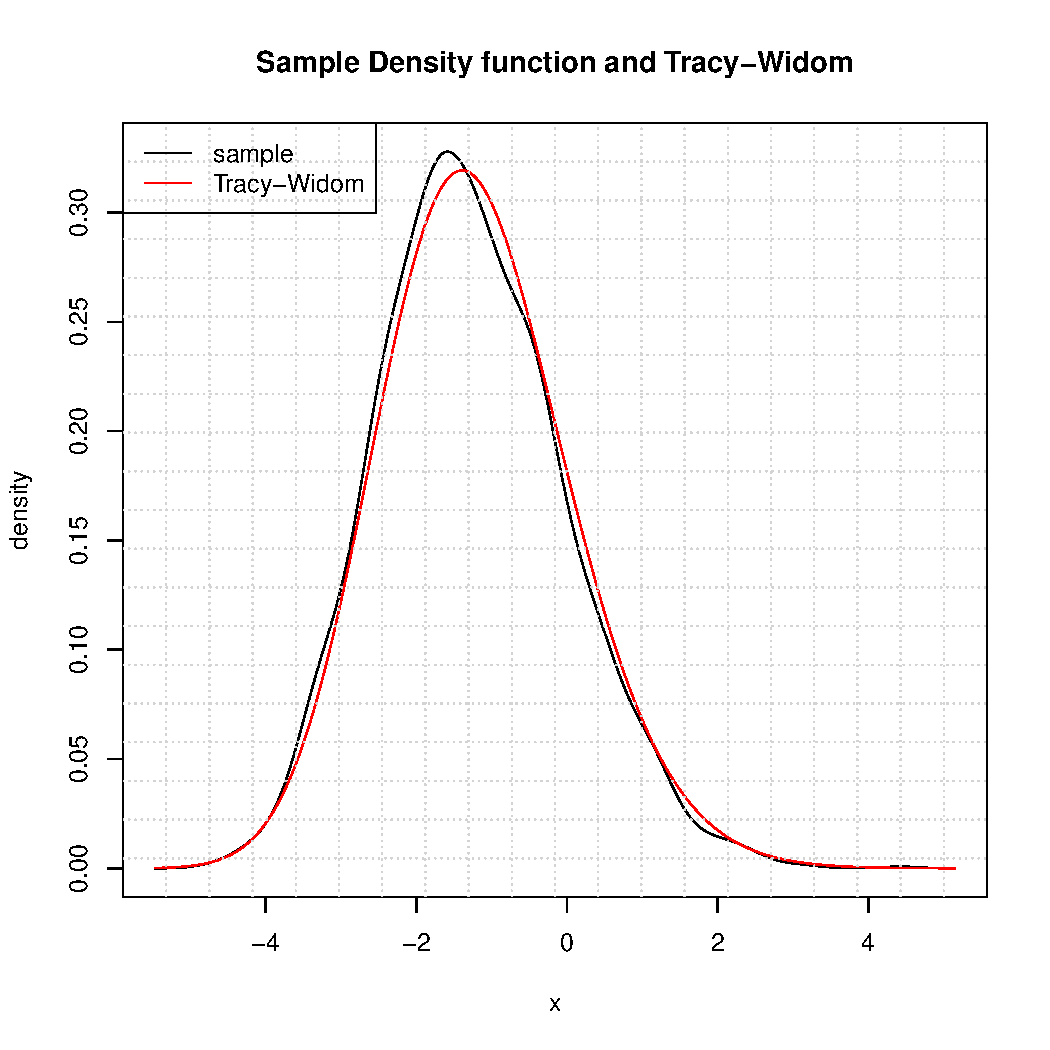
\includegraphics[scale=0.34]{normal-TW.pdf}
  }
  \subfigure[Entry distribution: $\P(X=\sqrt{3}) = \P(X=-\sqrt{3} ) =
  1/6$, $\P(X=0)=2/3$. Note $\E X = 0$, { $\E[ X^2] = 1$, $\E [X^3] = 0$ and
  $\E[ X^4] = 3$, i.e., the first 4 moments of $X$ match those of the standard normal \ds .}]{
    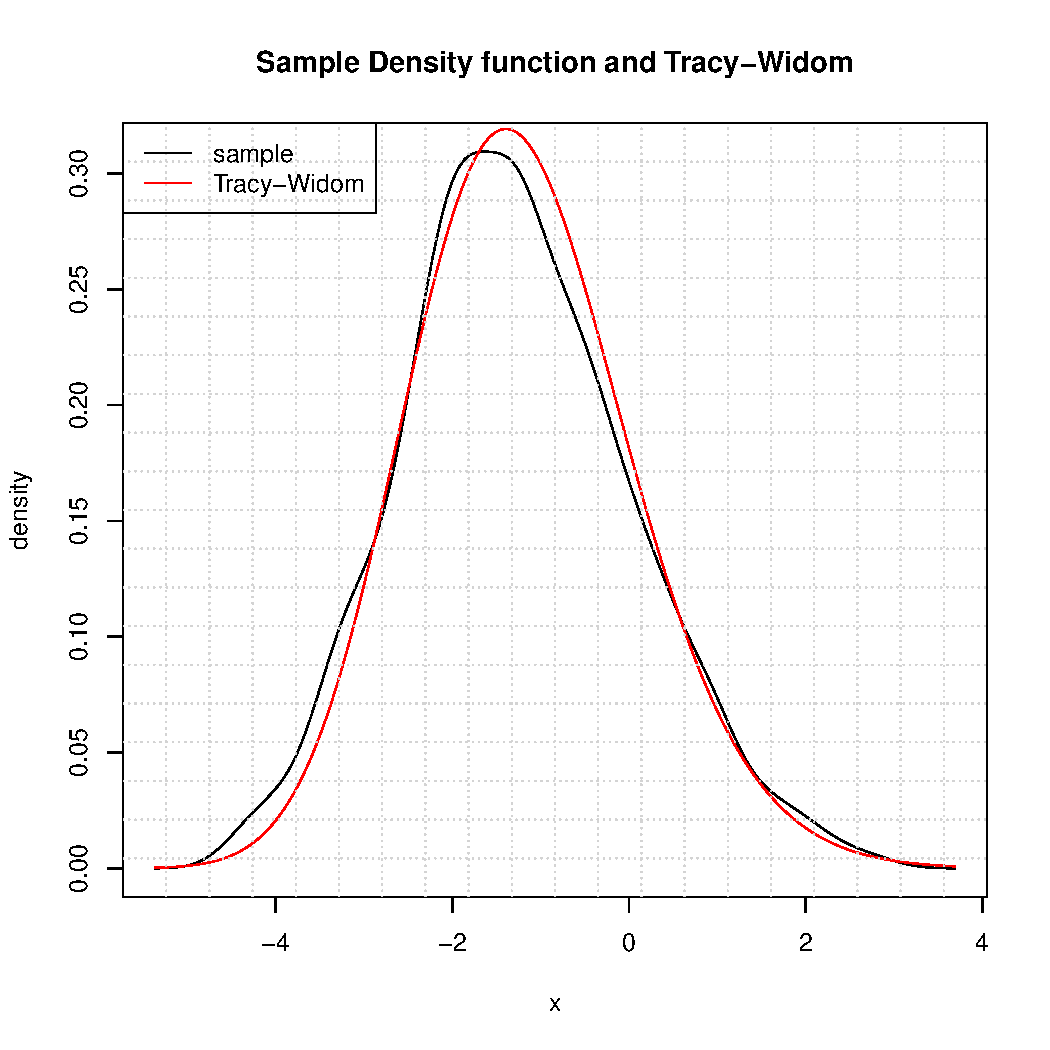
\includegraphics[scale=0.34]{3point-TW.pdf}
  }
  \caption{Sample density function of the largest eigenvalue compared
    with the Tracy--Widom density function. The data matrix $ \X$ has
    dimension $200 \times 1000$. An ensemble of 2000 matrices is
    simulated.}
  \label{fig:normal-3point-TW}
\end{figure}

Assuming \eqref{eq:gammach3} and iid entries $X_{it}$ with zero mean, unit variance and finite fourth moment,  Geman~\cite{geman}
showed that
\beam\label{eq:gemanch3}
\dfrac {\la_{(1)}}{n} \stas \big(1+\sqrt{\gamma}\big)^2\,,\qquad \nto\,.
\eeam
Johnstone \cite{johnstone:2001} complemented this \slln\ by the corresponding \clt\ in the special case of iid standard normal
entries:
\beam\label{eq:tcch3}
 n^{2/3}\,\dfrac{(\sqrt{\gamma})^{1/3}}{\big(1+\sqrt{\gamma}\big)^{4/3}}\Big(\dfrac {\la_{(1)}}{n} -
\big(1+\sqrt{\tfrac pn }\big)^2\Big)
\std {\rm TW}\,,
\eeam
where the limiting \rv\ has a {\em Tracy--Widom \ds} of order 1. Notice that the centering
$\big(1+\sqrt{\tfrac pn }\big)^2$ can in general not be replaced by $(1+\sqrt{\gamma})^2$.
This \ds\ is ubiquitous in random matrix theory.
%It is defined via some ordinary differential equation; we refer to \cite{tracy:widom:2012} for a definition and properties.
Its distribution function $F_1$ is given by
\begin{equation*}
F_1(s) = \exp\Big\{
  -\frac{1}{2} \int_{s}^\infty [
    q(x) + (x - s) q^2(x)
 ] \dint x
\Big\}\,,
\end{equation*}
where $q(x)$ is the unique solution to the Painlev\'e II differential
equation
\begin{equation*}
  q''(x) = xq(x) + 2 q^3(x)\,,
\end{equation*}
where $ q(x)\sim {\rm Ai}(x)$ as $x \to \infty$ and Ai$(\cdot)$ is the Airy kernel; see Tracy and Widom~\cite{tracy:widom:2012} for details.
We notice that the rate $n^{2/3}$ compares favorably to the $\sqrt{n}$-rate in the classical \clt\ for sums
of iid finite variance \rv s.
The calculation of the spectrum is facilitated by the fact that the distribution of
the classical Gaussian matrix ensembles is invariant under orthogonal transformations. The corresponding
computation for non-invariant matrices with non-Gaussian entries is more complicated and was a major challenge for several years; a first step was made by Johansson \cite{johansson}.
Johnstone's result was extended to matrices $\X$ with iid non-Gaussian entries
by Tao and Vu \cite[Theorem~1.16]{tao09b}. Assuming that the first four moments of the entry \ds\ match  those of
the standard normal \ds , they showed \eqref{eq:tcch3} by
employing {\em Lindeberg's replacement method}, i.e., the iid non-Gaussian entries are replaced
step-by-step by iid Gaussian ones.
This approach is well-known from summation theory for \seq s of iid \rv s. Tao and Vu's result is a consequence of the so-called {\em Four Moment Theorem}, which describes the insensitivity of the eigenvalues with respect to changes in the distribution of the entries. To some extent (modulo the strong moment matching conditions) it shows the universality of Johnstone's limit
result \eqref{eq:tcch3}. Later we will deal with entries with infinite fourth moment. In this case, the weak limit
for the normalized largest eigenvalue $\la_{(1)}$ is distinct from the Tracy--Widom \ds : the classical Fr\'echet extreme value
\ds\ appears.
In Figure~\ref{fig:normal-3point-TW} we illustrate how the Tracy--Widom approximation works for Gaussian and non-Gaussian entries of $\X$
and in Figure~\ref{fig:MyDist-Frechet} we also illustrate that this approach fails when $\E[X^4]=\infty$.


Figure \ref{fig:normal-3point-TW} compares the sample density function
of the properly normalized largest eigenvalue estimated from 2000 simulated sample covariance matrices $\X\X'$ ($n=1000, p=200$) with
the Tracy--Widom density. If  $X$ has infinite fourth moment and further regularity conditions on the tail hold then the
Tracy--Widom limiting law needs to be replaced by the \Frechet
distribution; see Section~\ref{subsec:1.2} for details. Figure \ref{fig:MyDist-Frechet} illustrates this fact with a
simulated ensemble whose entries are distributed according to
the heavy-tailed distribution from \eqref{eq:distrsimch3} below with $\alpha = 1.6$.
\begin{figure}[htb!]
  \centering
  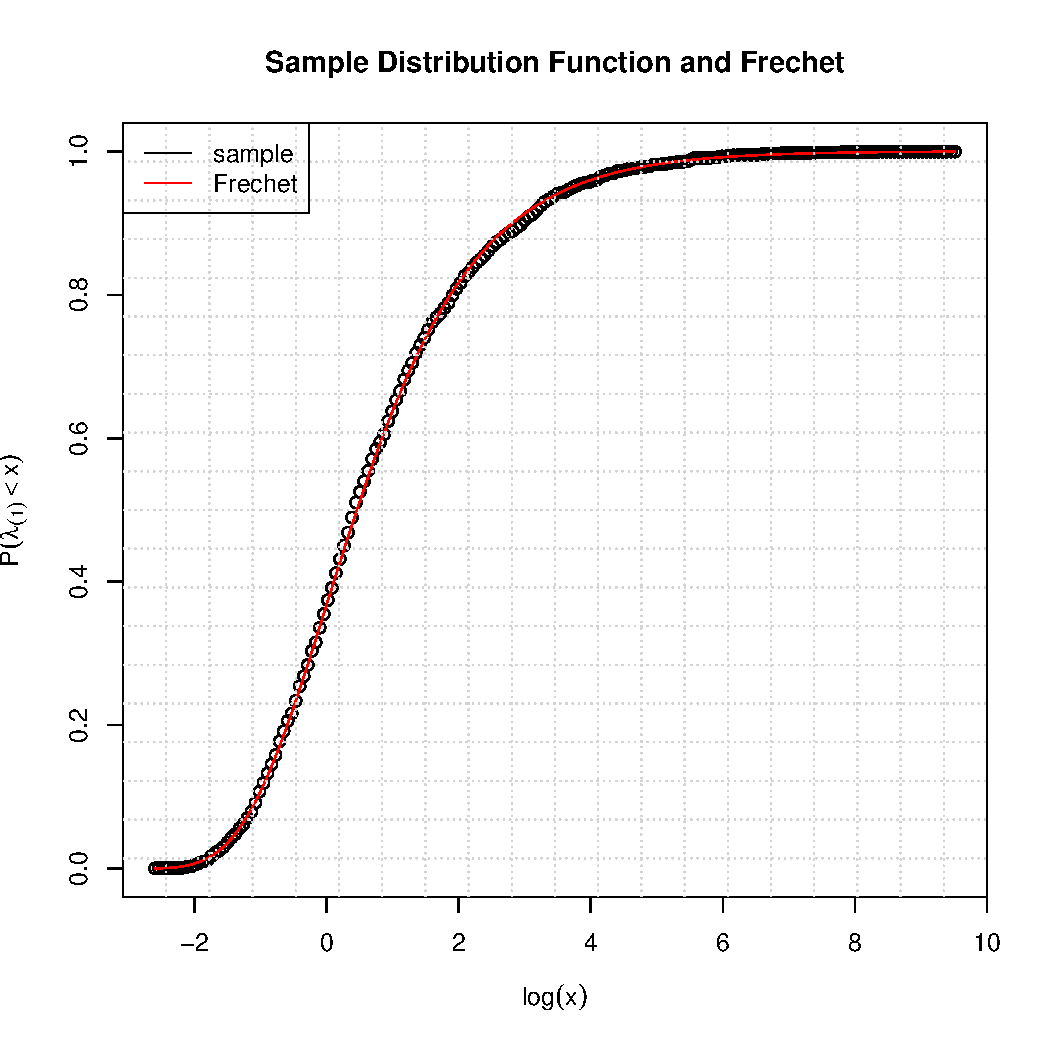
\includegraphics[scale=0.5]{MyDist-Frechet.pdf}
  \caption{Sample distribution function of the largest eigenvalue $\la_{(1)}$
    compared to the \Frechet distribution (solid line) with $\alpha=1.6$. The data matrices have dimension
    $200 \times 1000$ and iid entries with infinite fourth moment. The results are based on 2000 replicates.}
  \label{fig:MyDist-Frechet}
\end{figure}

\subsection{The heavy-tailed case}\label{subsec:1.2}
So far we focused on ``light-tailed'' $\X$
in the sense that its entries have finite fourth moment.  However, there is statistical evidence that the assumption
of finite fourth moment may be violated when dealing with data from
insurance, finance or telecommunications. We illustrate this fact
in Figure~\ref{fig:SP500_tail_indices} where we show the pairs $(\alpha_L,\alpha_U)$ of
lower and upper tail indices
of $p=478$  log-return series composing
the S\&P 500 index estimated from $n=1,345$ daily observations from 01/04/2010 to 02/28/2015.
This means we assume for every row  $(X_{it})_{t=1,\ldots,n}$ of $\X$ that the tails behave like
\beao
\P(X_{it}>x)\sim c_U\,x^{-\alpha_U}\qquad\mbox{and}\qquad \P(X_{it}<-x)\sim c_L\,x^{-\alpha_L}\,,\qquad \xto\,,
\eeao
for non-negative constants $c_L,c_U$. We apply the Hill estimator (see Embrechts et al.~\cite{embrechts:kluppelberg:mikosch:1997}, p.~330,
de Haan and Ferreira \cite{dehaan:ferreira:2006}, p.~69)
to the \ts\ of the gains and losses in a naive way,
neglecting the dependence and non-stationarity in the data; we also omit confidence bands.
From the figure it is evident that the majority of the return series have tail indices below
four, corresponding to an infinite fourth moment.
\begin{figure}[htb!]
\centering
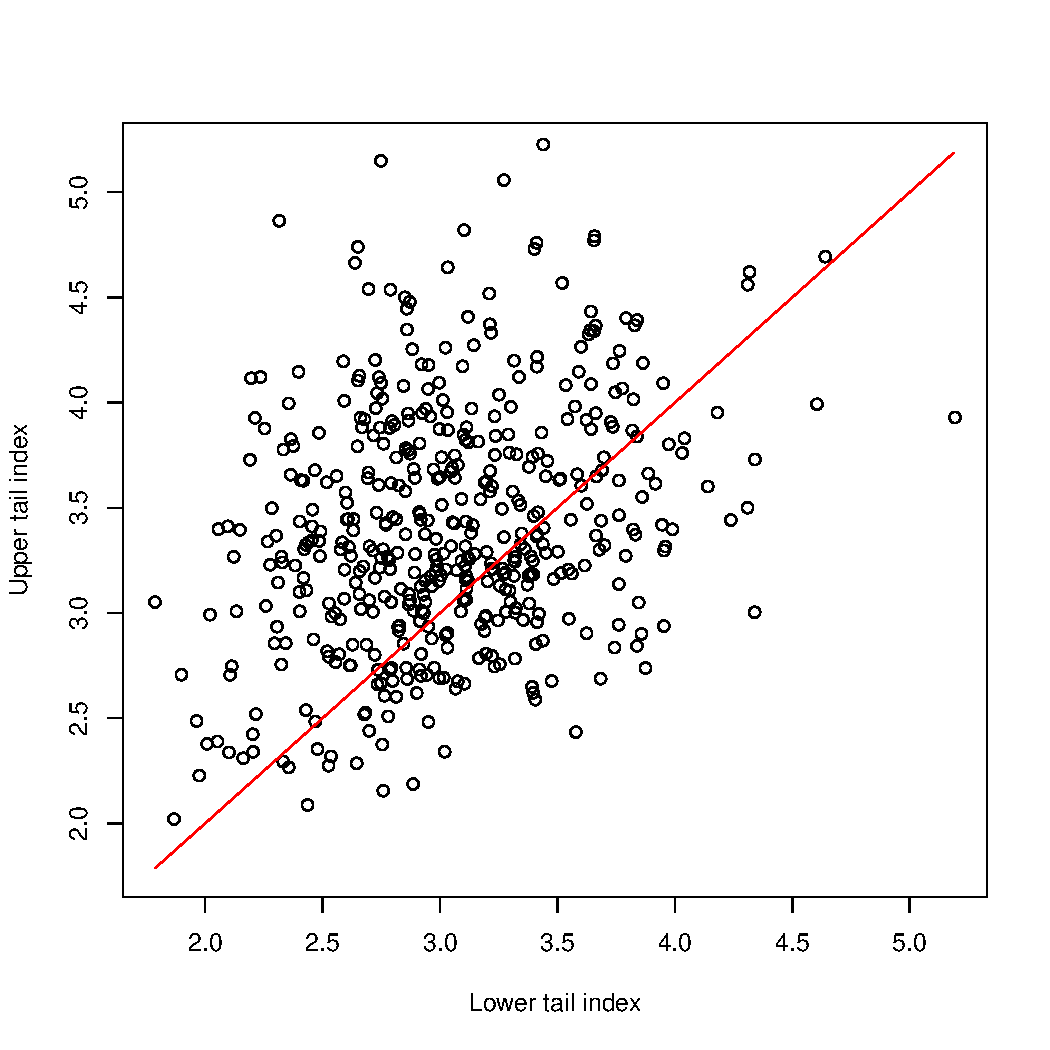
\includegraphics[scale=0.5]{SP500_tail_indices.pdf}
\caption{Tail indices of log-returns of 478 \ts\ from the S\&P 500 index. The values  $(\hat \alpha_L,\hat \alpha_U)$ of the
lower and upper tail indices are provided by
Hill's estimator.  We also draw the line $\hat\alpha_U=\hat\alpha_L$.}
\label{fig:SP500_tail_indices}
\end{figure}
The behavior of the largest eigenvalue $\la_{(1)}$
changes dramatically when $\X$ has infinite fourth moment.
Bai and Silverstein~\cite{baisilv} proved for an $n\times n$ matrix $\X$ with iid centered entries
that
\beam\label{eq:wdfrch3}
\limsup_{\nto} \dfrac{\la_{(1)}}{n}=\infty \qquad {\rm a.s.}
\eeam
This is in stark contrast to Geman's result \eqref{eq:gemanch3}.
%It is also unlikely that the
%Tracy--Widom \ds\ yields a good approximation to the \ds\ of the largest eigenvalue of the sample covariance matrix;
%see Figure~\ref{fig:MyDist-Frechet} for some simulation evidence.
\par
In the heavy-tailed case it is common to assume a {\em \regvar\ condition:}
\beam\label{eq:regvarch3}
\P(X>x)\sim p_+\,\dfrac{L(x)}{x^{\alpha}}\qquad\mbox{and}\qquad \P(X<-x) \sim p_-\,\dfrac{L(x)}{x^\alpha}\,,\qquad \xto\,,
\eeam
where $ p_\pm$ are non-negative constants \sth\ $p_++p_-=1$ and $L$ is a \slvary\ \fct . In particular, if $\alpha<4$ we have $\E [X^4]= \infty$. The \regvar\ condition
on $X$ (we will also refer to $X$ as a \regvary\ \rv ) is needed for proving \asy\ theory for
the eigenvalues of $\X\X'$. This is similar to proving limit theory for sums
of iid \rv s with infinite variance stable limits; see for example Feller~\cite{feller}.
\par

In \eqref{eq:MPch3} we have seen that the sequence $(F_{n^{-1}\X \X'})$ of empirical spectral distributions converges to the Mar\v cenko--Pastur law if the centered iid entries possess a finite second moment. Now we will discuss the situation when the entries are still iid and centered, but have an infinite variance. Here we assume the entries to be regularly varying with index $\alpha \in (0,2)$.
Assuming \eqref{eq:gammach3} with $\gamma\in (0,1]$ in this infinite variance case, Belinschi et al.~\cite[Theorem~1.10]{belinschi:dembo:guionnet:2009} showed that the sequence $(F_{a_{n+p}^{-2}\X \X'})$ converges with probability one to a non-random probability measure with density $\rho_{\alpha}^\gamma$ satisfying
\begin{equation*}
\rho_{\alpha}^\gamma(x) x^{1+\alpha/2} \to \frac{\alpha \gamma}{2(1+\gamma)}, \quad x \to \infty,
\end{equation*}
see also Ben Arous and Guionnet \cite[Theorem~1.6]{arous:guionnet:2008}.
The normalization $(a_k)$ is chosen \sth\ $\P(|X|>a_k)\sim k^{-1}$ as $k\to\infty$. An application of the Potter bounds (see Bingham et al. \cite[p.~25]{bingham:goldie:teugels:1987}) shows that $a_{n+p}^2/n \to \infty$.



It is interesting to note that there is a phase change in the extreme eigenvalues in going from finite to infinite fourth moment, while the phase change occurs for the empirical spectral distribution going from finite to infinite variance.
%In the case of finite fourth moment, \eqref{eq:geman} and \eqref{eq:MP} imply that $\lambda_{(k)}/n$ has to converge to the right endpoint of the Mar\v cenko--Pastur law for any finite $k$. However, if we assume an infinite fourth moment but finite second moment the empirical spectral distributions  $(F_{{n}^{-1}\X \X'})$ still converge to the Mar\v cenko--Pastur law with the same support, while $\lambda_{(1)}/n$ will tend to infintity due to \eqref{eq:wdfr}. This means that the proportion of the normalized eigenvalues taking values larger than $(1+\sqrt{\gamma})^2$ has to be negligible; otherwise we would have a contradiction to the convergence of the empirical spectral distributions to the Mar\v cenko--Pastur law.

%Finally, if the second moment is infinity, i.e.~regularly varying entries with index $\alpha \in (0,2)$, then the much larger values of the eigenvalues are visible in the limiting spectral distribution even when using a much stronger normalization \cite[Theorem~1.10]{belinschi:dembo:guionnet:2009}.
\par





The theory for the largest eigenvalues of sample covariance matrices with heavy tails is less developed than in the light-tailed case.
Pioneering work for $\la_{(1)}$ in the case of iid \regvary\ entries $X_{it}$ with index $\alpha\in (0,2)$
is due to Soshnikov~\cite{soshnikov:2004,soshnikov:2006}. He showed the \pp\ \con\
\beam\label{eq:nn}
N_n=\sum_{i=1}^p \vep_{a_{np}^{-2}\la_i} \std N=\sum_{i=1}^\infty \vep_{\Gamma_i^{-2/\alpha}}\,,\qquad \nto\,,
\eeam
under the growth condition \eqref{eq:gammach3} on $(p_n)$.
%The normalization $(a_k)$ is chosen \st\ $\P(|X|>a_k)\sim k^{-1}$ as $k\to\infty$.
Here
\beam\label{eq:Gamma}
\Gamma_i=E_1+\cdots + E_i\,,\qquad i\ge 1\,,
\eeam
and $(E_i)$ is an iid standard exponential \seq . In other words, $N$ is a Poisson point process on $(0,\infty)$ with mean \ms\
$\mu(x,\infty)= x^{-\alpha/2}$, $x>0$. Convergence in \ds\ of \pp es is understood in the sense of weak \con\
in the space of point \ms s equipped with the vague topology; see Resnick \cite{resnick:2007,resnick:1987}.
We can easily derive the limiting distribution of $a_{np}^{-2} \lambda_{(k)}$ for fixed $k\ge 1$ from \eqref{eq:nn}:
\begin{equation*}
\begin{split}
\lim_{\nto}\P(a_{np}^{-2} \lambda_{(k)}\le x)&= \lim_{\nto}\P(N_n(x,\infty)<k)
=  \P(N(x,\infty)<k) =\P(\Gamma_k^{-2/\alpha}\le x)\\ &= \sum_{s=0}^{k-1} \frac{\big(\mu(x,\infty)\big)^s}{s!} \e^{-\mu(x,\infty)}, \quad  x>0.
\end{split}
\end{equation*}
In particular,
\beao
\dfrac{\la_{(1)}}{a_{np}^2}\std \Gamma_1^{-\alpha/2}\,,\qquad \nto\,,
\eeao
where the limit has {\em Fr\'echet \ds } with parameter $\alpha/2$ and distribution function
\beao
\Phi_{\alpha/2}(x) =\ex^{-x^{-\alpha/2}}\,,\qquad x>0\,.
\eeao

\noindent We mention that the tail balance condition \eqref{eq:regvarch3} may be replaced in this case by the weaker assumption
$\P(|X|>x)= L(x) x^{-\alpha}$ for a \slvary\ \fct\ $L$. Indeed, it follows from the proof %(see also the comments below)
that only the squares $X_{it}^2$ contribute to the \pp\ limits of the eigenvalues $(\la_i)$. A con\seq\ of the
\cmt\ and \eqref{eq:nn} is the joint \con\ of the upper order statistics: for any $k\ge 1$,
\beao
a_{np}^{-2} \big(\la_{(1)},\ldots,\la_{(k)}\big)\std \big(\Gamma_1^{-2/\alpha},\ldots,\Gamma_k^{-2/\alpha}\big)\,,\qquad \nto\,.
\eeao

It follows from standard theory
for \pp es with iid points (e.g. Resnick \cite{resnick:2007,resnick:1987})
that \eqref{eq:nn} remains valid if
we replace  $N_n$  by the \pp\ $\sum_{i=1}^p\sum_{t=1}^n\vep_{X_{it}^2/a_{np}^2}$. Then we also have for any $k\ge 1$,
\beam\label{eq:nna}
a_{np}^{-2} \big(X_{(1),np}^2,\ldots,X_{(k),np}^2\big)\std \big(\Gamma_1^{-2/\alpha},\ldots,\Gamma_k^{-2/\alpha}\big)\,,\qquad \nto\,,
\eeam
where
\beao
X_{(1),np}^2\ge \cdots \ge X_{(np),np}^2
\eeao
denote the order statistics of $(X_{it}^2)_{i=1,\ldots,p;t=1,\ldots,n}$.
\par
Auffinger et al.~\cite{auffinger:arous:peche:2009} showed that \eqref{eq:nn}
remains valid under the \regvar\ condition \eqref{eq:regvarch3} for  $\alpha\in (2,4)$, the growth condition
\eqref{eq:gammach3} on $(p_n)$ and the
additional assumption $\E [X]=0$. Of course, \eqref{eq:nna} remains valid as well.
Davis et al.~\cite{davis:pfaffel:stelzer:2014} extended these results to the case when the rows of $\X$
are iid linear processes with iid \regvary\ noise. The Poisson \pp\ \con\ result of \eqref{eq:nn} remains valid in this case.
Different limit processes can only be expected if there is dependence across rows and columns.
\par
In what follows, we refer to the  {\em heavy-tailed case} when we assume the \regvar\ condition \eqref{eq:regvarch3}
for some $\alpha\in (0,4)$.%{\blue This hypothesis is confirmed in}

\subsection{Overview}

The primary objective of this overview  is to make a connection between extreme value theory and the behavior of the largest eigenvalues of sample covariance matrices from heavy-tailed multivariate time series.  For time series that are linearly dependent through time and across rows, it turns out that the extreme eigenvalues are essentially determined by the extreme order statistics from an array of iid random variables.  The asymptotic behavior of the extreme eigenvalues is then derived routinely from classical extreme value theory.  As such, explicit joint distributions of the extreme order statistics can be given which yield a plethora of ancillary results.  
%These include the limit behavior of ratios of consecutive extreme eigenvalues, ratios of extreme order statistics to the sample variance, etc..
%%The underlying multivariate \ts\ will assumed to be heavy-tailed and linearly dependent through time and across the rows.We consider asymptotic theory for the largest eigenvalues of a sample covariance matrix,
%and we will also address the largest singular values of the sample autocovariance matrix.
%To our knowledge, the present paper is the first to consider bonafide dependence among the components in the time series which renders a multivariate analysis, such as PCA, meaningful.
Convergence of the point process of extreme eigenvalues, properly normalized, plays a central role in establishing the main results.
\par
In Section~\ref{sec:2ch3} we continue the study of the case when the data matrix $\X$ consists of iid heavy-tailed entries.  We will consider power-law growth rates on the dimension $(p_n)$ that is more general than prescribed by \eqref{eq:gammach3}.
In Section~\ref{sec:model} we introduce a model for $X_{it}$ which allows for linear dependence across the rows and through time.
The point process convergence of normalized eigenvalues is presented in Section~\ref{sec:mainresult}.
This result lays the foundation for new insight into the spectral behavior of the sample covariance matrix, which is the content of Section~\ref{sec:samplecov}.

Sections~\ref{sec:samplecov} and \ref{sec:possemidef} are devoted to {\em sample autocovariance matrices}.  Motivated by \cite{lam:yao}, we study the eigenvalues of sums of transformed matrices and illustrate the results in two examples. These results are applied to the time series of S\&P 500 in Section \ref{sec:sp500}.
%The technical proofs are collected in Section~\ref{sec:proof}. 
Appendix~\ref{appendix:Ach3} contains useful facts about regular variation and point processes.




\section[General growth rates for $p_n$]{General growth rates for $p_n$ in the iid heavy-tailed case}\label{sec:2ch3}
This section is based on ideas in Heiny and Mikosch \cite{heiny:mikosch:2015:iid} where one can also find detailed proofs.
\subsection*{Growth conditions on $(p_n)$}\label{subsec:pn}
In many applications it is not realistic to assume
that the dimension $p$ of the data and the sample size $n$ grow at the same rate.
The aforementioned results of Soshnikov~\cite{soshnikov:2004,soshnikov:2006} and Auffinger et al. \cite{auffinger:arous:peche:2009} already indicate that the value $\gamma$ in the growth
rate~\eqref{eq:gammach3} does not appear in the \ds al limits.
This obervation is in contrast to the light-tailed case; see \eqref{eq:gemanch3}
and \eqref{eq:tcch3}.  Davis et al.~\cite{davis:mikosch:pfaffel:2015,davis:pfaffel:stelzer:2014}
and Heiny and Mikosch ~\cite{heiny:mikosch:2015:iid} allowed for more general rates for
$p_n\to\infty$ than linear growth in $n$.
Recall that $p=p_n\to\infty$ is the number of rows in the
matrix $\X_n$. We need to specify the growth rate of $(p_n)$ to ensure
a non-degenerate limit distribution of the normalized singular values of the sample autocovariance
matrices. To be precise, we assume
\begin{equation}\label{eq:pch3}
p=p_n=n^\beta \ell(n), \quad n\ge1,\tag{$C_p(\beta)$}
\end{equation}
where $\ell$ is a slowly varying function and $\beta\ge 0$. If $\beta =0$, we also assume $\ell(n) \to \infty$.
Condition~\ref{eq:pch3} is more general than the growth conditions in the literature; see
\cite{auffinger:arous:peche:2009,davis:mikosch:pfaffel:2015,davis:pfaffel:stelzer:2014}.
\begin{theorem}\label{thm:intro}
Assume that $\X=\X_n$ has iid entries satisfying the \regvar\ condition \eqref{eq:regvarch3} for some
$\alpha \in (0,4)$. If $\E[|X|]<\infty$ we also suppose that $\E [X]=0$. Let $(p_n)$ be an integer sequence
satisfying \ref{eq:pch3} with $\beta\ge 0$. In addition, we require
\begin{equation}\label{Cbeta}
\min(\beta,\beta^{-1})\in (\alpha/2-1,1] \qquad \mbox{ for } \alpha\in [2,4), \tag{$\widetilde{C}_\beta(\alpha)$}
\end{equation}
Then
\beam\label{eq:2}
\sum_{i=1}^p \vep_{a_{np}^{-2}\la_i}\std \sum_{i=1}^\infty \vep_{\Gamma_i^{-2/\alpha}}\,,\qquad \nto\,,
\eeam
where the \con\ holds in the space of point \ms s with state space $(0,\infty)$ equipped with the vague toplogy; see Resnick \cite{resnick:2007}.
\end{theorem}


\subsubsection*{A discussion of the case $\beta\in [0,1]$}
We mentioned earlier that in the heavy-tailed case, limit theory for the
largest eigenvalues of the sample covariance matrix is rather insensitive to
the growth rate of $(p_n)$ and that the limits are essentially
determined by the diagonal of this matrix. This is confirmed by the following result.

\begin{proposition}\label{prop:offdiagonalch3}
Assume that $\X=\X_n$ has iid entries satisfying the \regvar\ condition \eqref{eq:regvarch3} for some
$\alpha \in (0,4)$. If $\E[|X|]<\infty$ we also suppose that $\E [X]=0$. Then for any \seq\ $(p_n)$
satisfying \ref{eq:pch3} with $\beta\in [0,1]$ we have
\beao
a_{np}^{-2} \twonorm{\X \X' - \diag(\X \X')}\stp 0\,,\qquad\nto\,,
\eeao
where $\| \cdot\|_2$ denotes the spectral norm; see \eqref{specnorm} for its definition.
\end{proposition}


\par
Proposition~\ref{prop:offdiagonalch3} is not unexpected for two reasons:
\begin{itemize}
\item
It is well-known from classical theory (see Embrechts and Veraverbeke \cite{embrechts:veraverbeke:1982}) that for any iid \regvary\ non-negative \rv s
$Y,Y'$ with index  $\alpha'>0$, $Y\,Y'$ is \regvary\ with index $\alpha'$ while $Y^2$ is \regvary\ with index $\alpha'/2$.
Therefore $X^2$ and $X_{11}X_{12}$  are \regvary\ with indices $\alpha/2$ and $\alpha$, respectively.
\item
The aforementioned tail behavior is inherited by the entries of $\X\X'$ in the following sense.
By virtue of Nagaev-type \ld\ results for an iid \regvary\ \seq\ $(Y_i)$ with index $\alpha'\in (0,2)$ where we also assume that
$\E [Y_0]=0$ if $\E[|Y_0|]<\infty$
(see Theorem~\ref{thm:nagaevch3}) %S.V. Nagaev \cite{nagaev:1979} and
%Cline and Hsing \cite{cline:hsing:1998})
we have that $\P(Y_1+\cdots +Y_n >b_n)/(n \,\P(|Y_0|>b_n))$ converges to a non-negative constant
provided $b_n/a_n'\to\infty$, where $\P(|Y_0|>a_n')\sim n^{-1}$ as $\nto$. As a con\seq\ of the tail behaviors of $X_{it}^2$ and $X_{it}X_{jt}$ for $i\ne j$
and Nagaev's results we have for $(b_n)$ \sth\ $b_n/a_n^2\to\infty$,
\beam \label{eq:dfsdfjl}
\dfrac{\P\big((\X\X')_{ij}> b_n\big)}{\P\big((\X\X')_{ii}- c_n> b_n\big)}\sim \dfrac{n\,\P( X_{11}X_{12}>b_n)}{n\,\P(X^2>b_n)}\to 0\,,\qquad \nto\,,
\eeam
where $c_n=0$ or $n\,\E[X^2]$ according as $\alpha\in (0,2)$ or $\alpha\in (2,4)$.
This means that the diagonal and off-diagonal entries of
$\X\X'$ inherit the tails of $X_{it}^2$ and $X_{it}X_{jt}$, $i\ne j$, respectively, above the high threshold $b_n$.
\end{itemize}
\par
Proposition~\ref{prop:offdiagonalch3} has some immediate con\seq s for the approximation of the eigenvalues
of $\X\X'$ by those of ${\rm diag}(\X\X')$. Indeed, let $C$ be a symmetric $p\times p$ matrix with
eigenvalues $\la_1(C),\ldots,\la_p(C)$ and
ordered eigenvalues
\beam \label{eq:weyl}
\la_{(1)}(C)\ge \cdots \ge \la_{(p)}(C)\,.
\eeam
Then for any symmetric $p\times p$ matrices $A,B$, by {\em Weyl's inequality} (see Bhatia \cite{bhatia:1997}),
\beao
\max_{i=1,\ldots,p}\big|\la_{(i)}(A+B)-\la_{(i)}(A)\big|\le \|B\|_2\,.
\eeao
If we now choose
$A+B=\X\X'$ and $A= \diag (\X\X')$ we obtain the following result.
\begin{corollary}\label{cor:687ch3}
Under the conditions of Proposition~\ref{prop:offdiagonalch3},
\beao
a_{np}^{-2}\,\max_{i=1,\ldots,p}\big|\la_{(i)}-\la_{(i)}(\diag(\X\X'))\big|\stp 0\,,\quad\nto \,.
\eeao
\end{corollary}
Thus the problem of deriving limit theory for the order statistics of $\X\X'$ has been reduced to limit theory for the order
statistics of the iid row-sums
\beao
D_i^{\rightarrow}= (\X\X')_{ii}=\sum_{t=1}^n X_{it}^2\,,\qquad i=1,\ldots,p\,,
\eeao
which are the eigenvalues of $\diag(\X\X')$. This theory is completely described by the \pp es constructed from the points $D_i^\rightarrow/a_{np}^2$ $i=1,\ldots,p$. Necessary
and sufficient conditions for the weak \con\ of these \pp es are provided by  Lemma~\ref{lem:pprch3}
which in combination with the Nagaev-type \ld\ results of  Theorem~\ref{thm:nagaevch3}
yield the following result; see also Davis et al.~\cite{davis:mikosch:pfaffel:2015}.
\begin{lemma}\label{lem:ppch3}
Assume the conditions of Proposition~\ref{prop:offdiagonalch3} hold. Then
\beao
\sum_{i=1}^p \vep_{a_{np}^{-2}(D_i^\rightarrow-c_n)}\std \sum_{i=1}^\infty \vep_{\Gamma_i^{-2/\alpha}}\,,\qquad \nto\,,
\eeao
where $(\Gamma_i)$ is defined in \eqref{eq:Gamma} and $c_n=0$ if $\E[D^\rightarrow]=\infty$ and $c_n=\E[D^\rightarrow]$ otherwise.
\end{lemma}
In this result, centering is only needed for $\alpha\in [2,4)$ when $n/a_{np}^2\not\to 0$. Under the additional condition \ref{Cbeta},
%\begin{equation}\label{Cbetaor}
%\beta\in (\alpha/2-1,1], \quad \mbox{ for } \alpha\in [2,4),
%\end{equation}
$n/a_{np}^2\to 0$ in view of the Potter bounds; see Bingham et al. \cite[p.~25]{bingham:goldie:teugels:1987}.
Combining Lemma~\ref{lem:ppch3} and Corollary~\ref{cor:687ch3}, we conclude that Theorem~\ref{thm:intro} holds for $\beta\in [0,1]$.

%In  Davis et al. \cite{davis:mikosch:pfaffel;2015} relation \eqref{eq:2} was derived for $\alpha\in (0,1)$ even for \seq s
%$p_n\to\infty$ \st\ $p_n= O(\ex^{s_n/n})$, where $s_n=o(n)$ but with stronger limitations on the growth of $(p_n)$ for $[1,4]$.
%In the case $\alpha\in (2,4]$ they proved \eqref{eq:center} with $(\la_i)$ replaced by $(\la_i(\X\X'-n\E[ \X\X']))$. It is surprising that
%\eqref{eq:center} also holds since, in general, $\la_i(\X\X'-\E [\X\X'])\not = \la_i-n\,\E X$.


\subsubsection*{Extension to general $\beta$}%\label{subsec:generalb}
Next we explain that it suffices to consider only the case $\beta\in [0,1]$ and how to proceed when $\beta>1$.
The main reason is that
the $p \times p$ sample covariance matrix
$\X\X'$ and the $n \times n$ matrix $\X'\X$  have the same rank and their non-zero eigenvalues coincide; see Bhatia \cite[p.~64]{bhatia:1997}. When proving limit
theory for the eigenvalues  of the sample covariance matrix one may switch to $\X'\X$ and vice versa,
hereby interchanging the roles of $p$ and $n$. By switching to $\X'\X$, one basically replaces $\beta$ by $\beta^{-1}$. Since $\min(\beta,\beta^{-1})\in [0,1]$ for any $ \beta \ge 0$, one can assume without loss of generality that $\beta\in [0,1]$.  This trick allows one to extend results for
$(p_n)$ satisfying \ref{eq:pch3} with $\beta\in [0,1]$  to $\beta>1$. We illustrate this approach by providing the direct analogs of Proposition~\ref{prop:offdiagonalch3} and Corollary~\ref{cor:687ch3}.


\begin{proposition}\label{prop:offdiagonal1}
Assume that $\X=\X_n$ has iid entries satisfying the \regvar\ condition \eqref{eq:regvarch3} for some
$\alpha \in (0,4)$. If $\E[|X|]<\infty$ we also suppose that $\E [X]=0$. Then for any \seq\ $(p_n)$
satisfying \ref{eq:pch3} with $\beta>1$ we have
\beao
a_{np}^{-2} \twonorm{\X' \X - \diag(\X' \X)}\stp 0\,,\qquad\nto\,,
\eeao
where $\| \cdot\|_2$ denotes the spectral norm.
\end{proposition}
Note that for $\beta>1$ we have $\lim_{\nto} p/n= \infty$. This means that
$\X'\X$ has  asymptotically a much smaller dimension than $\X\X'$ and therefore it is more convenient to work with $\X' \X$
when bounding the spectral norm.
\begin{corollary}\label{cor:6871}
Under the conditions of Proposition~\ref{prop:offdiagonal1},
\beao
a_{np}^{-2}\,\max_{i=1,\ldots,n}\big|\la_{(i)}-\la_{(i)}(\diag(\X'\X))\big|\stp 0\,,\quad\nto \,.
\eeao
\end{corollary}
Now, Theorem~\ref{thm:intro} for $\beta > 1$ is a consequence of Corollary~\ref{cor:6871}.
\par

%-----------------------------------------------------------------------
\section{Introducing dependence between the rows and columns}\label{sec:model}
For details on the results of this section, we refer to Davis et al.~\cite{davis:mikosch:pfaffel:2015}, Heiny and Mikosch \cite{heiny:mikosch:2015:iid} and Heiny et al.~\cite{heiny:mikosch:2016:noniid}. 

\subsection{The model}
When dealing with covariance matrices of a multivariate \ts\ $(\X_n)$ it is rather natural to assume dependence
between the entries $X_{it}$.
In this section we introduce a model which allows for {\em linear dependence}
between the rows and columns of $\X$:
\begin{equation}\label{eq:1}
X_{it}=\sum_{l\in \Z}\sum_{k\in \Z} h_{kl} Z_{i-k,t-l}\,,\qquad i,t\in\Z\,,
\end{equation}
where $(Z_{it})_{i,t\in \Z}$ is a field of iid \rv s and $(h_{kl})_{k,l\in\Z}$ is an array of real numbers.
Of course, linear dependence is restrictive in some sense. However, the particular dependence structure allows one to
determine those ingredients in the sample covariance matrix which contribute to its largest eigenvalues.
If the series in \eqref{eq:1} converges a.s. $(X_{it})$ constitutes a strictly stationary random field.
We denote generic elements of the $Z$- and $X$-fields by $Z$ and $X$, respectively. We assume that $Z$ is \regvary\ in the sense that
\begin{equation}\label{eq:27}
\P(Z>x)\sim p_+ \dfrac{L(x)}{x^{\alpha}}\quad\mbox{and}\quad  \P(Z\le -x)\sim p_-
\dfrac{L(x)}{x^{\alpha}}\,,\qquad \xto\,,
\end{equation}
for some tail index $\alpha>0$, constants $p_+,p_-\ge 0$ with $p_++p_-=1$ and a \slvary\ $L$. We will assume $\E[ Z]=0$ whenever $\E [Z^2]<\infty$.
Moreover, we require the summability condition
\begin{equation}\label{eq:2a}
\sum_{l \in \Z} \sum_{k\in \Z} |h_{kl}|^{\delta} <\infty
\end{equation}
for some $\delta\in (0,\min({\alpha/2},1))$ which ensures
the a.s.~absolute convergence of the series in \eqref{eq:1}. Under the conditions \eqref{eq:27} and \eqref{eq:2a}, the marginal and
\fidi s of the field $(X_{it})$ are \regvary\ with index $\alpha$; see
Embrechts et al. \cite{embrechts:kluppelberg:mikosch:1997}, Appendix A3.3. Therefore we also refer to $(X_{it})$ and $(Z_{it})$
as \regvary\ fields.
\par
The model \eqref{eq:1} was introduced by Davis et al. \cite{davis:pfaffel:stelzer:2014}, assuming the rows iid, and in the
present form by Davis et al. \cite{davis:mikosch:pfaffel:2015}.
\subsection{Sample covariance and autocovariance matrices}
From the field $(X_{it})$ we construct the $p\times n$ matrices
\begin{equation}\label{eq:26}
\X_n(s)= (X_{i,t+s})_{i=1,\ldots,p;t=1,\ldots,n}\,,\qquad s=0,1,2,\ldots\,,
\end{equation}
As before, we will write $\X=\X_n(0)$.
Now we can introduce the (non-normalized)
{\em sample autocovariance matrices}
\beam\label{eq:sample}
\X_n(0)\X_n(s)'\,,\qquad s=0,1,2,\ldots\,.
\eeam
We will refer to $s$ as the {\em lag}. For $s=0$, we obtain the {\em sample covariance matrix.}
In what follows, we will be interested in the asymptotic behavior (of \fct s) of the eigen- and singular values of the
sample covariance and autocovariance matrices in the heavy-tailed case. Recall that the {\em singular values} of a matrix $A$ are the square roots of the
eigenvalues of the non-negative definite matrix $AA'$ and its {\em spectral norm} $\twonorm{A}$ is its largest singular value. We notice that $\X_n(0)\X_n(s)'$ is not symmetric
and therefore its eigenvalues can be complex. To avoid this situation, we use
%\beao
%\X_n(0)\X_n(s)' +\X_n(s)\X_n(0)'
%\eeao
%(this matrix is symmetric and therefore it has real eigenvalues) or use
the squares
\beam\label{eq:squares}
\X_n(0)\X_n(s)' \X_n(s)\X_n(0)'
\eeam
%(this matrix is  non-negative definite  and therefore it has non-negative eigenvalues).
whose eigenvalues are the squares of the singular values of $\X_n(0)\X_n(s)'$.
The idea of using the sample autocovariance matrices and \fct s of their squares \eqref{eq:squares}
originates from a paper by Lam and Yao~\cite{lam:yao} who used a model different from \eqref{eq:1}.
This idea is quite natural in the context of \tsa .
\par
In Theorem~\ref{thm:mains} below, we provide a general approximation result for the ordered singular values of the sample
autocovariance matrices in the heavy-tailed case. This result is rather technical. To formulate it we introduce further notation.
As before, $p=p_n$ is any integer \seq\ converging to infinity.
\subsection{More notation}
Important roles are played by the quantities $(Z_{it}^2)_{i=1,\ldots,p;t=1,\ldots,n}$ and their order statistics
 \begin{equation}\label{eq:zorderch3}
Z_{(1),np}^2 \ge Z_{(2),np}^2 \ge  \ldots \ge Z_{(np),np}^2, \qquad n,p\ge 1\,.
\end{equation}
As important are the row-sums
\begin{equation}\label{eq:llch3}
D_i^\rightarrow=D_i^{(n),\rightarrow}=\sum_{t=1}^n Z_{it}^2\,, \qquad
i=1,\ldots,p;\quad  n=1,2,\ldots\,,
\end{equation} with generic element $D^\rightarrow$ and their ordered values
\beam\label{eq:help6ch3}
D_{(1)}^\rightarrow=D_{L_1}^\rightarrow\ge \cdots \ge D_{(p)}^\rightarrow=D_{L_p}^\rightarrow\,,
\eeam
where we assume without loss of generality that $(L_1,\ldots,L_p)$ is
a permutation of $(1,\ldots,p)$ for fixed~$n$.
\par
Finally, we introduce the column-sums
\beao
D_t^\downarrow=D_t^{(n),\downarrow}= \sum_{i=1}^p Z_{it}^2\,,\qquad t=1,\ldots,n;\; \quad p=1,2,\ldots\,,
\eeao
with generic element $D^\downarrow$ and we also adapt the notation from \eqref{eq:help6ch3} to these quantities.
\subsubsection*{Matrix norms} For any $p\times n $ matrix $\A=(a_{ij})$, we will use the following norms:
\begin {itemize}
\item
{\em Spectral norm:}
\beam\label{specnorm}
\|\A\|_2=\sqrt{\la_{(1)}(\A\A')}\,,
\eeam
\item
{\em Frobenius norm:}
\beao
\frobnorm{\A}= \Big( \sum_{i=1}^p \sum_{j=1}^n |a_{ij}|^2\Big)^{1/2}\,.
\eeao
%\item
%{\em Max-row sum norm:}
%\beao
%\inftynorm{A}= \max_{i=1,\ldots,p} \sum_{j=1}^n |a_{ij}|\,.
%\eeao
%\item
%{\em Max-column sum norm:}
%\beao
%\|{A}\|_1 = \max_{j=1,\ldots,n} \sum_{i=1}^p |a_{ij}|\,.
%\eeao
\end{itemize}
We will frequently make use of the bound $\|\A\|_2\le \|\A\|_ F$. Standard references for matrix norms are \cite{belitski,bhatia:1997, horn, shores}.
\subsubsection*{Singular values of the sample autocovariance matrices} Fix integers $n\ge 1$ and $s\ge 0$. We recycle the $\la$-notation
for the singular values
$\la_1(s), \ldots, \la_p(s)$ of the sample autocovariance matrix $\X_n(0)\X_n(s)'$, suppressing the dependence on $n$.
Correspondingly, the  order statistics are denoted by
\begin{equation}\label{eq:sigma}
\la_{(1)}(s) \ge \cdots \ge \la_{(p)}(s)\,.
\end{equation}
When $s=0$ we typically write $\la_i$ instead of $\la_i(0)$.
\subsubsection*{The matrix $\M(s)$} We introduce some auxiliary matrices
derived from the coefficient matrix $\H=(h_{kl})_{k,l\in \Z}$:
\beao
\H(s)=(h_{k,l+s})_{k,l\in \Z}, \qquad \M(s)= \H(0)\H(s)'\qquad s\ge 0\,.
\eeao
Notice that
\begin{equation}\label{eq:m}
(\M(s))_{ij}= \sum_{l\in \Z} h_{i,l} h_{j,l+s}, \qquad i,j \in \Z .
\end{equation}
We denote the ordered singular values of $\M(s)$ by
\begin{equation}\label{eq:v1}
v_1(s) \ge v_2(s) \ge\cdots \,.
\end{equation}
Let $r(s)$ be the rank of $\M(s)$ so that $v_{r(s)}(s)>0$ while $v_{r(s)+1}(s)=0$ if $r(s)$ is
finite, otherwise $v_i(s)>0$ for all $i$. We also write $r=r(0)$.
\par
Under the summability condition \eqref{eq:2a} on $(h_{kl})$ for fixed $s\ge 0$,
\beam\label{eq:tracea}
\sum_{i=1}^\infty (v_i(s))^2 &=&  \frobnorm{\M(s)}^2= \sum_{i,j\in \Z} \sum_{l_1,l_2 \in \Z} h_{i,l_1} h_{j,l_1+s}h_{i,l_2}
h_{j,l_2+s}\nonumber\\
&\le& c \,\Big(\sum_{l_1,l_2 \in \Z} \sum_{i\in \Z} |h_{i,l_1} h_{i,l_2}|\Big)^2
\le c \,\sum_{l_1\in \Z} \sum_{i \in \Z} |h_{i,l_1}| <\infty\,.
\eeam
Therefore all singular values $v_i(s)$ are finite and the ordering
  \eqref{eq:v1}
is justified.
\par
{\em Here and in what follows, we write $c$ for any constant whose value is not of interest.}

\subsubsection*{Normalizing sequence}
We define $(a_k)$ by
\beao
\P(|Z|>a_k)\sim k^{-1}\,,\qquad k\to\infty\,,
\eeao
and choose the normalizing \seq\ for the singular values as $(a_{np}^2)$ for suitable \seq s $p=p_n\to\infty$.
\subsubsection*{Approximations to singular values}\label{subsec:defdelta}
We will give approximations to the singular values $\la_i(s)$  in
terms of the  $p$ largest ordered values for $s\ge 0$,
\beao
&&\delta_{(1)}(s)\ge \cdots \ge \delta_{(p)}(s)\,,\\
&&\gamma_{(1)}^\rightarrow(s)\ge \cdots \ge \gamma_{(p)}^\rightarrow(s)\,,\\
&&\gamma_{(1)}^\downarrow(s)\ge \cdots \ge \gamma_{(n)}^\downarrow(s)\,,
\eeao
from the sets
\beao
&&\big\{Z_{(i),np}^2 v_j(s)\,, i=1,\ldots,p\,;j=1,2,\ldots\big\}\,,\notag\\
&&\big\{D_{i}^\rightarrow v_j(s), i=1,\ldots,p\,;j=1,2,\ldots\big\}\,,\notag\\
&&\big\{D_{t}^\downarrow v_j(s), t=1,\ldots,n\,;j=1,2,\ldots\big\}\,,
\eeao
respectively.
%---------------------------------------------------------------------------
\subsection{Approximation of the singular values}\label{sec:mainresult}
%Furthermore, let $\tau_{(1)}(s)  \ge \ldots \ge \tau_{(p)}(s)$ be  the singular values of $\tfrac{1}{2}(\X_n(0)\X_n(s)'+\X_n(s)\X_n(0)' )$ and let $\tilde{\tau}_{(1)}(s) \ge  \ldots \ge\tilde{\tau}_{(p)}(s)$ be the singular values of
%\begin{equation*}
%\tfrac{1}{2}(\X_n(0)\X_n(s)'-\E[\X_n(0)\X_n(s)']+\X_n(s)\X_n(0)' -\E[\X_n(s)\X_n(0)'])
%\end{equation*}
In the following result we povide some useful approximations to the singular values of the sample autocovariance matrices of
the linear model \eqref{eq:1}.
\begin{theorem}\label{thm:mains}
Consider the linear process \eqref{eq:1} under
\begin{itemize}
\item
the \regvar\ condition \eqref{eq:27}
for some $\alpha\in (0,4)$,
\item the centering condition
$\E[Z]=0$ if $\E[|Z|]<\infty$,
\item
the summability condition
\eqref{eq:2a} on the coefficient matrix  $(h_{kl})$,
\item
the growth condition \ref{eq:pch3} on $(p_n)$ for some $\beta\ge 0$.
\end{itemize}
Then the following statements hold for $s\ge 0$:
\begin{enumerate}
\item We consider two disjoint cases:
$\alpha \in (0,2)$ and $\beta\in (0,\infty)$, or
$\alpha\in [2,4)$ and $\beta$ satisfying \ref{Cbeta}. Then
\begin{equation}\label{eq:mains1}
a_{np}^{-2} \max_{i=1,\ldots,p} |\la_{(i)}(s)-\delta_{(i)}(s)| \cip 0, \quad \nto.
\end{equation}
\item
Assume $\beta\in [0,1]$.
If $\alpha \in (0,2]$, $\E[Z^2]=\infty$ or $\alpha\in [2,4)$, $\E [Z^2]<\infty$ and $\beta\in (\alpha/2-1,1]$ then
\beao
a_{np}^{-2} \max_{i=1,\ldots,p} |\la_{(i)}(s)-\gamma_{(i)}^\rightarrow(s)| \cip 0, \quad \nto.
\eeao
Assume $\beta>1$. If $\alpha \in (0,2]$, $\E[Z^2]=\infty$ or $\alpha\in [2,4)$, $\E [Z^2]<\infty$ and $\beta^{-1}\in(\alpha/2-1,1]$. Then
\beao
a_{np}^{-2} \max_{i=1,\ldots,p} |\la_{(i)}(s)-\gamma_{(i)}^\downarrow(s)| \cip 0, \quad \nto.
\eeao
\end{enumerate}
\end{theorem}
\begin{remark}\em
The proof of Theorem~\ref{thm:mains} is given in Heiny et al.~\cite{heiny:mikosch:2016:noniid}. Part (2) of this  result
with more restrictive conditions on the growth rate of $(p_n)$ is contained in Davis et al.~\cite{davis:mikosch:pfaffel:2015}.
These proofs are very technical and lengthy.
\end{remark}
\begin{remark}\em
If we consider a random array $(h_{kl})$ independent of  $(X_{it})$ and
assume that the summability
condition \eqref{eq:2a} holds a.s.
then Theorem~\ref{thm:mains} remains valid conditionally on
$(h_{kl})$, hence  unconditionally in $\P$-probability; see also \cite{davis:mikosch:pfaffel:2015}.\end{remark}
\subsection{Point process \con }\label{sec:lkasfj}
Theorem~\ref{thm:mains}  and arguments similar to the proofs in Davis et al. \cite{davis:mikosch:pfaffel:2015}
enable one to derive the weak \con\ of
the point processes of the normalized singular values. Recall
the representation of the points $(\Gamma_i)$ of a unit rate homogeneous Poisson process on $(0,\infty)$
given in \eqref{eq:Gamma}. For $s\ge 0$, we define the point processes of the normalized singular values:
\begin{equation}\label{eq:ppdef}
N_n^{\lambda,s}=\sum_{i=1}^p \vep_{a_{np}^{-2}(\lambda_{(i)}(0),\ldots,\lambda_{(i)}(s))} \,.
\end{equation}

\begin{theorem}\label{cor:1ch3}
Assume the conditions of Theorem~\ref{thm:mains}.
Then $(N_n^{\lambda,s})$ converge weakly in the space of point measures
with state space $(0,\infty)^{s+1}$ equipped with the vague topology.
If either $\alpha \in (0,2]$, $\E[Z^2]=\infty$ and $\beta \ge 0$,
or $\alpha \in [2,4)$, $\E[Z^2]<\infty$ and \ref{Cbeta} hold then
\begin{equation}\label{eq:pp}
N_n^{\lambda,s} \cid N= \sum_{i=1}^\infty
\sum_{j=1}^{\infty} \vep_{\Gamma_i^{-2/\alpha} (v_j(0),\ldots,v_j(s))}, \qquad \nto.
\end{equation}
\end{theorem}

\begin{proof}
Regular variation of $Z^2$ is equivalent to
\begin{equation}\label{eq:wwa}
n\,p\, \P(a_{np}^{-2} Z^2  \in \cdot ) \civ \mu(\cdot),
\end{equation}
where $\civ$ denotes vague convergence of Radon measures on  $(0,\infty)$ and the \ms\ $\mu$ is given by $\mu(x,\infty)=x^{-\alpha/2}$, $x>0$.
In view of Resnick \cite{resnick:1987}, Proposition~3.21, \eqref{eq:wwa} is equivalent
to the weak \con\ of the following \pp es:
\begin{equation*}
\sum_{i=1}^p\sum_{t=1}^n \vep_{a_{np}^{-2} Z_{it}^2}=\sum_{i=1}^{np} \vep_{a_{np}^{-2} Z^2_{(i),np}}\cid
\sum_{i=1}^\infty\vep_{\Gamma_i^{-2/\alpha} }=\widetilde{N}\,,\quad
\nto\,,
\end{equation*}
where the limit $\widetilde{N}$ is a Poisson random measure (PRM) with state space $(0,\infty)$ and
mean measure~$\mu$.
\par
Since $a_{np}^{-2} Z^2_{(p),np}\cip 0$ as $\nto$,
the point processes $\sum_{i=1}^{p} \vep_{a_{np}^{-2} Z^2_{(i),np}}$ converge weakly to the same PRM:
\begin{equation}\label{eq:ppc}
\sum_{i=1}^{p} \vep_{a_{np}^{-2} Z^2_{(i),np}}\cid
\sum_{i=1}^\infty\vep_{\Gamma_i^{-2/\alpha} }\,,\quad
\nto\,.
\end{equation}
A continuous mapping argument together with the fact that $\sum_{i=1}^\infty (v_i(s))^2<\infty$ (see  \eqref{eq:tracea})
shows that
\begin{equation*}
\sum_{j=1}^{ \infty}\sum_{i=1}^p\vep_{a_{np}^{-2} Z^2_{(i),np}(v_j(0),\ldots,v_j(s))}\cid
\sum_{j=1}^{ \infty}\sum_{i=1}^\infty\vep_{\Gamma_i^{-2/\alpha}  (v_j(0),\ldots,v_j(s))}\,.
\end{equation*}
If the assumptions of part (1) of Theorem~\ref{thm:mains} are satisfied
an application of \eqref{eq:mains1} (also recalling the definition of $(\delta_{(i)}(s))$) shows that \eqref{eq:ppc} remains
valid with the points  $(a_{np}^{-2} Z^2_{(i),np}(v_j(0),\ldots,v_j(s)))$ replaced by
$(a_{np}^{-2} (\lambda_{(i)}(0),\ldots,\lambda_{(i)}(s))$.
\par
The only cases which are not covered by Theorem~\ref{thm:mains}(1) are $\alpha\in (0,2)$, $\beta=0$ and $\alpha=2$, $\E[Z^2]=\infty$, $\beta\ge0$.
In these cases we get from Theorem~\ref{thm:nagaevch3} that
\begin{equation*}
 p \, \P(a_{np}^{-2} D^\rightarrow>x ) \sim p\,n\, \P( Z^2>a_{np}^{2} x )\to \mu(x,\infty)\,,\quad x>0\,,
\end{equation*}
i.e., $
 p \, \P(a_{np}^{-2} D^\rightarrow\in \cdot ) \stackrel{v}{\rightarrow} \mu(\cdot)$.
It follows from Lemma~\ref{lem:pprch3} that
$\sum_{i=1}^p\vep_{a_{np}^{-2} D_i^\rightarrow}\std \widetilde{N}$. As before,
a continuous mapping argument in combination with
the approximation obtained in Theorem~\ref{thm:mains}(2)
justifies the replacement of the points $(a_{np}^{-2} D_{(i)}^\rightarrow(v_j(0),\ldots,v_j(s)))$ by
$(a_{np}^{-2} (\lambda_{(i)}(0),\ldots,\lambda_{(i)}(s)))$ in the case $\beta\in [0,1]$. If $\beta>1$ one has to work with the
quantities $(D_i^\downarrow)_{i=1,\ldots,n}$ instead of  $(D_i^\rightarrow)_{i=1,\ldots,p}$ and one may follow the same argument as above.
This finishes the proof.
\end{proof}

\section{Some applications}
\subsection{Sample covariance matrices}\label{sec:samplecov}%\setcounter{equation}{0}
The sample covariance matrix $\X_n(0)\X_n(0)'=\X\X'$ is a non-negative definite matrix. Therefore
its eigenvalues and singular values coincide.  Moreover, $v_j=v_j(0)$, $j\ge 1$, are the eigenvalues of $\M=\M(0)$.
\par
Theorem~\ref{thm:mains}(1) yields an approximation of the ordered eigenvalues $(\la_{(i)})$ of $\X\X'$ by
the quantities $(\delta_{(i)})$ which are derived from the order statistics of $(Z_{it}^2)$.
Part (2) of this result provides an approximation of $(\la_{(i)})$ by the quantities
$(\gamma_{(i)}^{\rightarrow/\downarrow})$ which are derived from the order statistics
of the partial sums $(D_i^{\rightarrow/\downarrow})$.
\par
In the following example we illustrate the
quality of the two approximations.
\begin{example}\label{ex:xiao}\em
We choose a Pareto-type \ds\ for $Z$ with density
\beam\label{eq:distrsimch3}
f_Z(x) =
\left\{\begin{array}{cc}
 \frac{\alpha}{(4|x|)^{\alpha + 1}}\,, & \mbox{if } |x| > 1/4 \\
1\,, & \mbox{otherwise.}
\end{array}\right.
\eeam
We simulated $20,000$ matrices $\X_n$ for $n=1,000$ and $p=200$ whose
iid entries have this density. We assume $\beta=1$.
Note that $\M=\M(0)$ has rank one and $v_1=1$.
The estimated densities of the deviations $a_{np}^{-2}(\lambda_{(1)}-D_{(1)}^\rightarrow)$ and
$a_{np}^{-2}(\lambda_{(1)}-Z^2_{(1),np})$  based on the simulations are shown in
Figure~\ref{fig:lambda_comparisonch3}. The approximation error is very small indeed.
\begin{figure}[htb!]
  \centering
  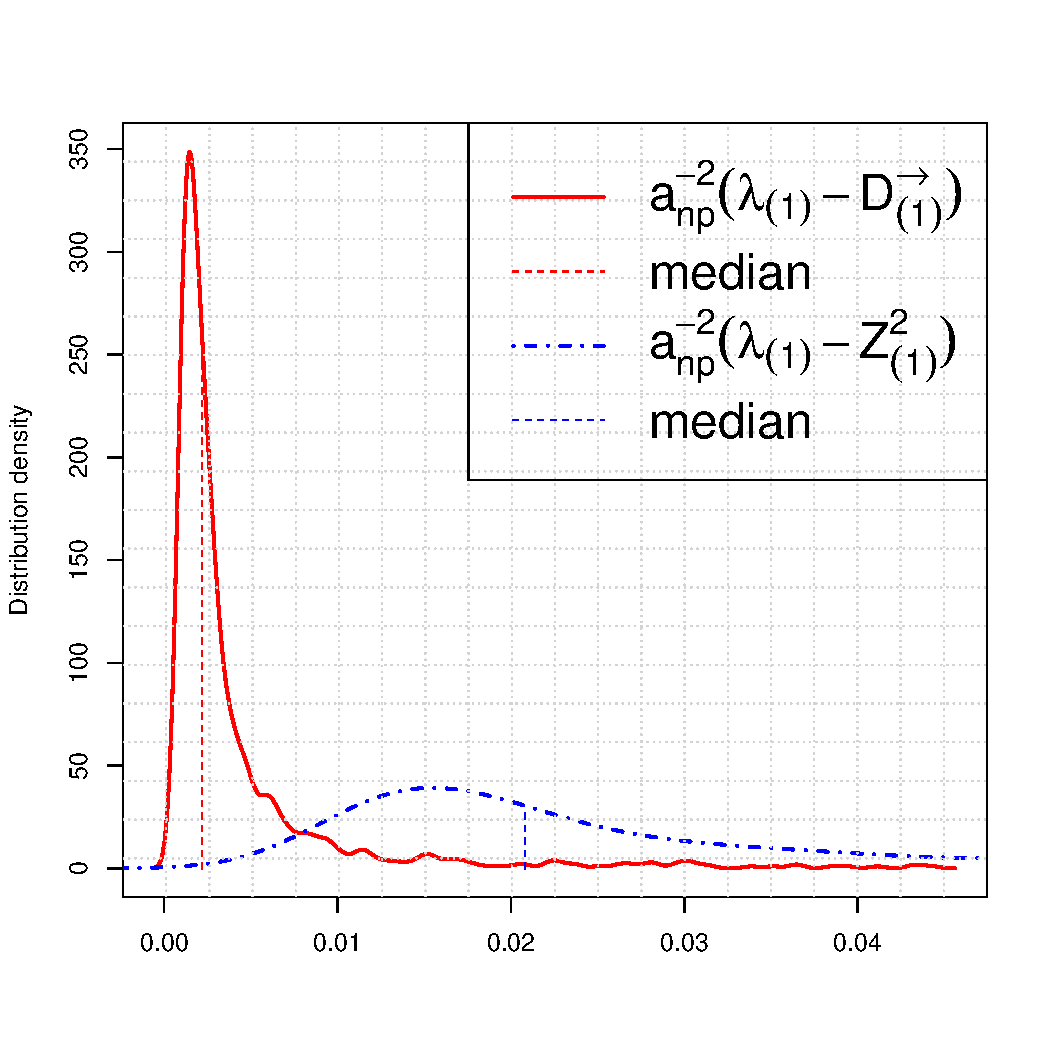
\includegraphics[scale=0.40]{lambda_comparison.pdf}
  \caption{Density of the approximation errors for the eigenvalues of $a_{np}^{-2}\X\X'$.
The entries of $\X$ are iid with density \eqref{eq:distrsimch3} and $\alpha=1.6$.}
  \label{fig:lambda_comparisonch3}
\end{figure}
According to the theory,
\beao
a_{np}^{-2}\sup_i|D_{(i)}^\rightarrow-\lambda_{(i)}| +a_{np}^{-2}\sup_i |Z^2_{(i),np}-\lambda_{(i)}|\stp 0\,,
\eeao
but  for finite $n$ the $(D_{(i)}^\rightarrow)$ sequence yields a better approximation to $(\la_{(i)})$. By construction,
the considered differences
have a tendency to be positive but Figure~\ref{fig:lambda_comparisonch3} also shows that the median of the
approximation error for $a_{np}^{-2}(\lambda_{(1)}-D_{(1)}^\rightarrow)$ is almost zero.
\end{example}
\par
Theorem~\ref{cor:1ch3} and the continuous mapping theorem immediately yield results about
the joint convergence of the largest eigenvalues of the matrices $a_{np}^{-2}\X_n\X_n'$ for $\alpha\in (0,2)$ and
$\alpha\in (2,4)$ when $\beta$ satisfies \ref{Cbeta}.
For fixed $k\ge 1$ one gets
\begin{equation*}
a_{np}^{-2} \big(\la_{(1)},\ldots,\la_{(k)}\big)\cid
\big(d_{(1)},\ldots, d_{(k)}\big)\,,
\end{equation*}
where $d_{(1)}\ge \cdots\ge d_{(k)}$ are the $k$ largest ordered
values of the set $\{\Gamma_i^{-2/\alpha} v_j, i=1,2,\ldots,j=1,\ldots,r\}$.
The continuous mapping theorem yields for $k\ge 1$,
\begin{equation}\label{eq:u}
\dfrac{\la_{(1)}}{\la_{(1)}+\cdots+ \la_{(k)}}\cid
\dfrac{d_{(1)}}{d_{(1)}+\cdots+ d_{(k)}}\,,\quad \nto\,.
\end{equation}

An application of the continuous mapping theorem to  the distributional convergence of the point processes in Theorem~\ref{cor:1ch3} in the spirit of Resnick
\cite{resnick:2007}, Theorem 7.1, also yields the following result; see Davis et al. \cite{davis:mikosch:pfaffel:2015} for a proof and a similar result in the case $\alpha \in (2,4)$.
\begin{corollary}\label{cor:1q} Assume the conditions of Theorem~\ref{thm:mains}.
If $\alpha \in (0,2]$ and $\E[Z^2]=\infty$, then
\begin{equation*}
a_{np}^{-2}\Big(\la_{(1)},\sum_{i=1}^p \la_i\Big) \cid
\Big( v_1\,\Gamma_1^{-2/\alpha}\,,\sum_{j=1}^r v_j\,\sum_{i=1}^\infty \Gamma_i^{-2/\alpha}\Big)\,,
\end{equation*}
where $\Gamma_1^{-2/\alpha}$ is Fr\'echet $\Phi_{\alpha/2}$-distributed.
and $\sum_{i=1}^\infty \Gamma_i^{-2/\alpha}$ has the distribution
of a positive $\alpha/2$-stable random variable.
In particular,
\begin{equation}\label{eq:limit}
\dfrac{\la_{(1)}}{\la_{1}+\cdots+ \la_{p}}\cid
\dfrac{v_1}{\sum_{j=1}^r v_j}\;
\dfrac{\Gamma_1^{-2/\alpha}}{\sum_{i=1}^\infty\Gamma_i^{-2/\alpha}}\,,\quad
\nto\,.
\end{equation}
\end{corollary}

\begin{remark}\label{rem:4.5}\em
The ratio
\begin{equation*}
\dfrac{\la_{(1)}+\cdots +\la_{(k)}}{\la_1+\cdots+\la_p}, \qquad k\ge 1\,,
\end{equation*}
plays an important role in PCA. It reflects the proportion of the total variance in the data that we can explain by the first $k$ principal components.
It follows from Corollary~\ref{cor:1q} that for fixed $k\ge 1$,
\begin{equation*}
\dfrac{\la_{(1)}+\cdots \la_{(k)}}{\la_1+\cdots+\la_p}\cid
\dfrac{d_{(1)}+\cdots +d_{(k)}} {d_{(1)}+d_{(2)}+\cdots}\,.
\end{equation*}
Unfortunately, the limiting variable does in general not have a clean
form.
An exception is the case when $r=1$; see Example~\ref{exam:separable}.
Also notice that the trace of $\X\X'$ coincides with $\la_1+\cdots+\la_p$.
\end{remark}



To illustrate the theory we consider a simple moving average example
taken from Davis et al.~\cite{davis:mikosch:pfaffel:2015}.
\begin{example} \rm
\begin{figure}[htb!]
  \centering
  \subfigure[iid data]{
    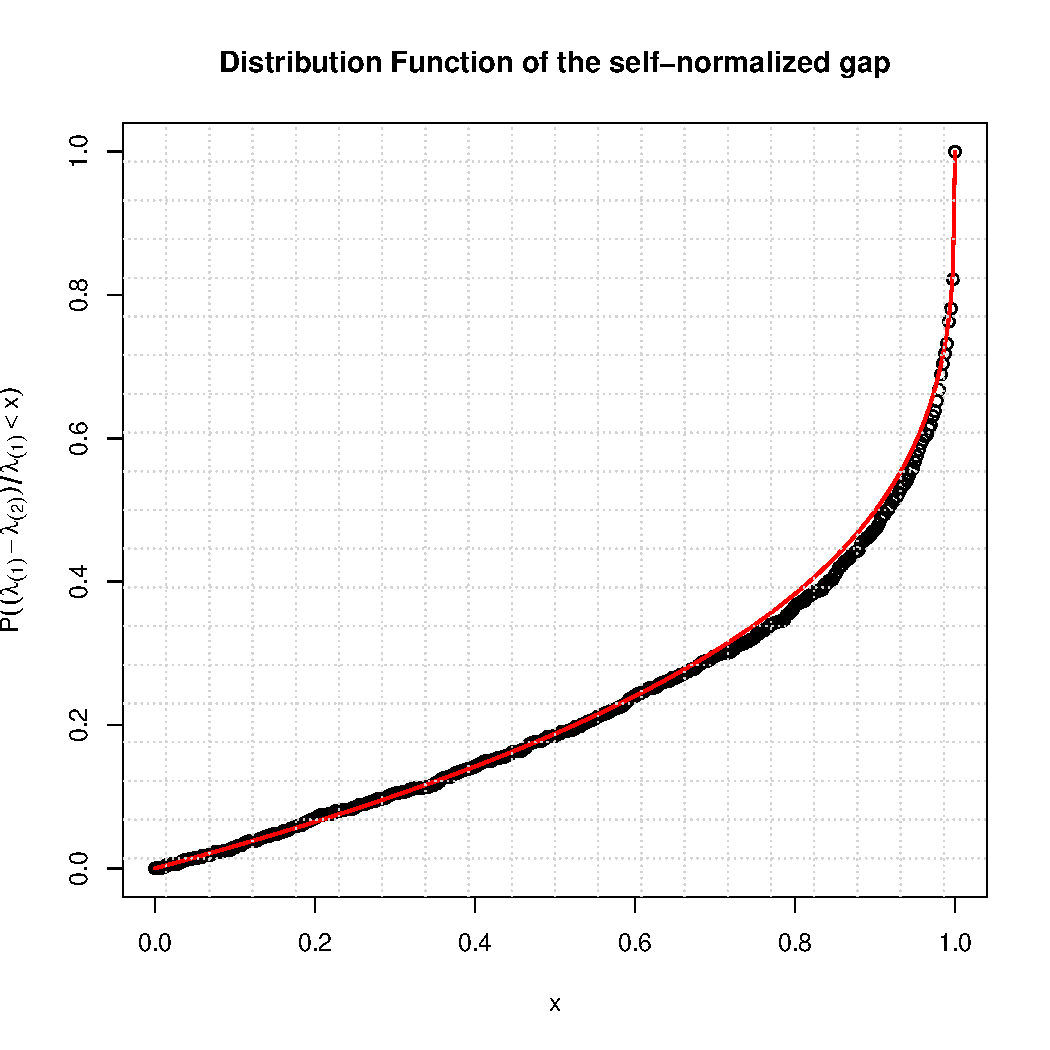
\includegraphics[scale=0.34]{lambda_1_2_Gaps_iid.pdf}
  }
  \subfigure[data from model \eqref{ex:4.6}]{
    \includegraphics[scale=0.34]{lambda_1_2_Gaps.pdf}
  }
  \caption{Distribution function of $(\lambda_{(1)} - \lambda_{(2)})/\lambda_{(1)}$ for iid data (left) and
    data generated from the model \eqref{ex:4.6} (right). In each graph we compare the empirical \ds\ \fct\
(dotted line, based on
1000 simulations of $200 \times 1000$ matrices with $Z$-\ds\ \eqref{eq:distrsimch3}) with the theoretical curve (solid line).}
  \label{fig:ProbMass}
\end{figure}
Assume that $\alpha\in (0,2)$ and
\begin{equation}\label{ex:4.6}
X_{it}= Z_{it}+ Z_{i,t-1}-2 (Z_{i-1,t}- Z_{i-1,t-1})\,,\quad i,t\in\Z\,.
\end{equation}
In this case, the non-zero entries of $\H$ are
\begin{equation*}
h_{00}=1, h_{01}=1,h_{10}=-2 \quad \mbox{ and }\quad h_{11}=2.
\end{equation*}
Hence $\M=\H\H'$ has the positive eigenvalues
$v_1=8$ and $v_2=2$. The limit point process in \eqref{eq:pp} is
\begin{equation*}
N=\sum_{i=1}^\infty \vep_{8\Gamma_i^{-2/\alpha}}+ \sum_{i=1}^\infty \vep_{2\Gamma_i^{-2/\alpha}}\,,
\end{equation*}
so that
\begin{equation*}
a_{np}^{-2}\,\big(\la_{(1)},\la_{(2)}\big) \cid
\big(8\Gamma_{1}^{-2/\alpha}, 2\Gamma_1^{-2/\alpha}\vee 8
\Gamma_2^{-2/\alpha}\big)\,.
\end{equation*}
Using the fact that $U=\Gamma_1/\Gamma_2$ has a uniform \ds\ on $(0,1)$ we calculate
\begin{equation*}
\P(2\Gamma_1^{-2/\alpha}>8\Gamma_2^{-2/\alpha})= \P(\Gamma_1/\Gamma_2<2^{-\alpha})= 2^{-\alpha} \in (1/4,1).
\end{equation*}
In particular, we have for the normalized spectral gap
\begin{equation*}
a_{np}^{-2} \big(\la_{(1)}-\la_{(2)}\big)\cid
6 \,\Gamma_1^{-2/\alpha} \1_{\{\Gamma_1 4^{\alpha/2 }<\Gamma_2\}}+
8\,
\big(\Gamma_1^{-2/\alpha}-\Gamma_2^{-2/\alpha}\big)\1_{\{\Gamma_14^{\alpha/2
  }> \Gamma_2\}}
\end{equation*}
and for the self-normalized spectral gap (see also Example~\ref{exam:spectralgap} for a detailed analysis)
\begin{equation*}
\begin{split}
\dfrac{\la_{(1)}-\la_{(2)}}{\la_{(1)}}&\cid
\dfrac{6}{8} \, \1_{\{\Gamma_1 2^{\alpha }<\Gamma_2\}}+
\big(1-(\Gamma_1/\Gamma_2)^{2/\alpha}\big)\1_{\{\Gamma_12^{\alpha
  }> \Gamma_2\}}\\
& =\dfrac{3}{4}\,  \1_{\{U 2^{\alpha }<1\}}+
\big(1-U^{2/\alpha}\big)\1_{\{U2^{\alpha
  }> 1\}}=Y\,.
\end{split}
\end{equation*}
The limit  distribution of the spectral gap
has an atom at $3/4$ with probability $2^{-\alpha}$, i.e.,~$\P(Y=3/4)=2^{-\alpha}$, and
\begin{equation*}
\P(Y\le x)= 1- (1-x)^{\alpha/2},\qquad x\in (0,3/4).
\end{equation*}
In the iid case the limit distribution of the self-normalized spectral gap has distribution function $F(x) = 1- (1-x)^{\alpha/2}$ for $x\in [0,1]$. This means that the atom disappears if the entries are iid. Figure~\ref{fig:ProbMass} compares the distribution function of $Y$
with $F$ for $\alpha=0.6$; the atom at $3/4$ is clearly visible.

Along the same lines, we also have
\begin{equation*}
(a_{np}^{-2}\lambda_{(1)},\lambda_{(2)}/\lambda_{(1)}) \cid(
8\,\Gamma_1^{-2/\alpha},\frac{1}{4}\,\1_{\{U<2^{-\alpha}\}}+U^{2/\alpha}\,\1_{\{U\ge
  2^{-\alpha}\}})\,
\end{equation*}
and hence the limit distribution of $\lambda_{(2)}/\lambda_{(1)}$ is supported on $[1/4,1)$ with  mass of $2^{-\alpha}$ at $1/4$.  The histogram of the ratio $\left(\lambda_{(2)}/\lambda_{(1)}\right)^{2/\alpha}$ based on 1000 replications from the model \eqref{ex:4.6} with noise given by a $t$-distribution with $\alpha=1.5$ degrees of freedom, $n=1000$ and $p=200$ is displayed in Figure \ref{fig:1}.
\begin{figure} [h]
\begin{center}
\includegraphics[scale=.35]{histogram.pdf}
\end{center}
\caption{Histogram based on 1000 replications of $\left(\lambda_{(2)}/\lambda_{(1)}\right)^{2/\alpha}$ from model \eqref{ex:4.6}.}
\label{fig:1}
\end{figure} Observing that $2^{-\alpha}=0.3536\ldots$,
the histogram is remarkably close to what one would expect from a sample from the truncated
uniform \ds , $2^{-\alpha}\, \1_{\{U<2^{-\alpha}\}}+U\, \1_{\{U\ge 2^{-\alpha} \}}$.
The mass of the limiting discrete component of the ratio can be much
larger if one conditions on $a_{np}^{-2}\lambda_{(1)}$ being large.
Specifically, for any $\epsilon\in (0,1/4)$ and $x>0$,
\begin{equation*}
\lim_{n\to\infty} \P(\epsilon<\lambda_{(2)}/\lambda_{(1)}\le 1/4|\lambda_{(1)}>a_{np}^2x)
=\P(\Gamma_1/\Gamma_2\le 2^{-\alpha}|\Gamma_1<(x/8)^{-\alpha/2})=G(x)\,.
\end{equation*}
The function $G$ approaches $1$ as $x\to\infty$ indicating the speed at which the
two largest eigenvalues get linearly related; see Figure \ref{fig:2} for a graph of $G$ in the case $\alpha=1.5$.
\begin{figure} [h]
\begin{center}
\includegraphics[scale=.35]{Hfunction.pdf}
\end{center}
\caption{Graph of $G(x)=\P(\Gamma_1/\Gamma_2\le2^{-\alpha}|\Gamma_1<(x/8)^{-\alpha/2})$ when $\alpha=1.5$.}
\label{fig:2}
\end{figure}
In addition, from Remark~\ref{rem:4.5}, we also have
\begin{equation*}
\dfrac{\la_{(1)}}{\la_1+\cdots +\la_p} \cid \dfrac{4}{5}\,
\dfrac{\Gamma_1^{-2/\alpha}}{\sum_{i=1}^\infty \Gamma_i^{-2/\alpha}}\,.
\end{equation*}
Clearly, the limit \rv\ is stochastically smaller than what one would get in the iid case; see \eqref{eq:limit}.
\end{example}
\begin{example}\label{exam:spectralgap}\rm
The previous example also illustrates the behavior of the two largest eigenvalues in the general case
when the rank $r$ of the matrix $\M$ is larger than one.
We have in general
\begin{equation*}
\dfrac{\lambda_{(2)}}{\lambda_{(1)}}\cid
\frac{v_2}{v_1}\,\1_{\{U<(v_2/v_1)^{\alpha/2}\}}+U^{2/\alpha}\,\1_{\{U\ge (v_2/v_1)^{\alpha/2}\}}\,.
\end{equation*}
In particular, the limiting
{\em self-normalized spectral gap} has \rep
\beao
\dfrac{\la_{(1)}-\la_{(2)}}{\la_{(1)}} \cid \dfrac{v_1-v_2}{v_1}\,\1_{\{U<(v_2/v_1)^{\alpha/2}\}}+(1-U^{2/\alpha})\,\1_{\{U\ge (v_2/v_1)^{\alpha/2}\}}\,.
\eeao
The limiting variable assumes values in $(0,1-v_2/v_1]$  and has an atom at the right end-point.
This is in contrast to the iid case
and to the case when $r=1$ (hence $v_2=0$) including the case of iid rows and the separable case; see Example~\ref{exam:separable}.
\end{example}
\begin{example}\label{exam:separable}
{\em We consider the separable case when  $h_{kl}=\theta_kc_l$, $k,l \in \Z$, where $(c_l)$, $(\theta_k)$ are
  real sequences such that the conditions on $(h_{kl})$ in
  Theorem~\ref{thm:mains} hold. In this case,
\begin{equation*}
\M= \sum_{l\in \Z} c_l^2\;\; (\theta_i\theta_j)_{i,j \in \Z}\,.
\end{equation*}
Note that $r=1$ with the only non-negative eigenvalue
\beao
v_1=\sum_{l\in \Z} c_l^2\;\;\sum_{k\in \Z}\theta_k^2\,.
\eeao
In this
case, the limiting point process in Theorem~\ref{cor:1ch3} is a PRM on
$(0,\infty)$ with mean measure of $(y,\infty)$ given by $(v_1/
y)^{\alpha/2}$, $y>0$. The normalized eigenvalues have similar asymptotic behavior as
in the case of iid entries. For example, the log-spacings have the same limit as in the iid case for fixed $k$,
\beao
\big(\log \la_{(1)}-\log \la_{(2)},\ldots,\log \la_{(k+1)}-\log \la_{(k)}\big)\std
-\dfrac{2}{\alpha}\,\big(\log(\Gamma_1/\Gamma_2),\ldots,\log (\Gamma_{k}/\Gamma_{k+1})\big)\,.
\eeao
The same observation applies to the ratio of the largest eigenvalue and the trace in the case $\alpha\in (0,2)$:
\beao
\dfrac{\la_{(1)}}{{\rm tr} (\X \X')}=\dfrac{\la_{(1)}}{\la_1+\cdots +\la_p} \std
\dfrac{\Gamma_1^{-2/\alpha}}{\sum_{i=1}^\infty \Gamma_i^{-2/\alpha}}\,.
\eeao
We also mentioned in Example~\ref{exam:spectralgap} that the \ds al limit of the self-normalized spectral gap has no atom
as in the iid case.
}
\end{example}

\subsection{S\&P 500 data}\label{sec:sp500}
We conduct a short analysis of the largest eigenvalues of the univariate log-return time series which compose
the S\&P 500 stock index; see Section~\ref{subsec:1.2} for a description of the data.
Although there is strong empirical evidence that these univariate series have power-law tails
(see Figure~\ref{fig:SP500_tail_indices}) we  do not expect that they
have the same tail index. One way to proceed would be to ignore this fact because the tail indices are
in a close range and the differences are due to large sampling errors for estimating such quantities.  One could also collect \ts\ with similar
tail indices in the same group.
In this case, the dimension $p$ decreases. This grouping would be a rather arbitrary classification method.
We have chosen a third way: to use rank transforms.
This approach has its merits because it aims at standardizing the tails but it also has a major disadvantage: one destroys
the covariance structure underlying the data.
\par
Given a $p\times n$ matrix $(R_{it})_{i = 1, \cdots, p;t=1,\cdots, n}$,
we construct a matrix $\X$ via the rank transforms
\begin{equation*}
  X_{it} = -\Big[
    \log \Big(\frac{1}{n+1} \sum_{\tau=1}^n \1_{\{R_{i\tau} \leq R_{it}\}} \Big)
  \Big]^{-1} \,,\qquad i=1,\ldots,p;t=1,\ldots,n\,.
\end{equation*}
\begin{figure}[htb!]
  \centering
    \includegraphics[scale=0.550]{EigenRatioSP500_ranks_log_50_shown.pdf}
  \caption{The logarithms of the ratios $\lambda_{(i+1)} / \lambda_{(i)}$ for the S\&P 500 series after rank transform.
We also show the 1, 50 and 99\% quantiles (bottom, middle, top lines, respectively) of the variables
$\log((\Gamma_i/ \Gamma_{i+1})^{2})$. }
  \label{fig:EigenRatio}
\end{figure}
\begin{figure}[htb!]
  \centering
    \includegraphics[scale=0.550]{EigenRatioSP500_log_50_shown.pdf}
  \caption{The logarithms of the ratios $\lambda_{(i+1)} / \lambda_{(i)}$ for the original (non-rank transformed) S\&P 500 log-return data.
We also show the 1, 50 and 99\% quantiles (bottom, middle, top lines, respectively) of the variables
$\log((\Gamma_i/ \Gamma_{i+1})^{2/2.3})$; see also Figure~\ref{fig:EigenRatio} for comparison.}\label{fig:22}
\end{figure}

%\begin{figure}[htb!]
%  \centering
%    \includegraphics[scale=0.550]{EigenRatioSP500_lin2_250_shown.pdf}
%  \caption{{\green Same as Figure \ref{fig:EigenRatio} but on original scale, no logarithm. Choose one.}}
%\end{figure}

If the rows $R_{i1}, \ldots, R_{in}$ were iid (or, more generally, stationary ergodic)
with a continuous \ds\  then
the averages under the logarithm would be  asymptotically uniform
on $(0,1)$ as $n \to \infty$. Hence $X_{it}$ would  be \asy ally standard
Fr\'echet $\Phi_1$-distributed.
In what follows, we assume that the aforementioned univariate \ts\ of the S\&P 500 index have undergone the rank transform and that
their marginal \ds s are close to $\Phi_1$; we
always use the symbol $\X$ for the resulting multivariate series.
\par
In Figure~\ref{fig:EigenRatio} we show the ratios of the consecutive ordered eigenvalues $(\la_{(i+1)}/\la_{(i)})$
of the matrix $\X\X'$. This graph shows the rather surprising fact that the ratios are close to one even for small values $i$.
We also show the 1, 50 and 99 \% quantiles of the variables $((\Gamma_{i}/\Gamma_{i+1})^{2/\alpha})$ calculated from the formula
\beam\label{eq:iid}
\P\big((\Gamma_{i} /\Gamma_{i+1})^{2/\alpha}\le x \big) = x^{i \cdot \alpha/2}, \quad x\in (0,1)\,.
\eeam
For increasing $i$, the \ds\ is concentrated closely to 1, in agreement with the \slln\ which yields
$\Gamma_{i} /\Gamma_{i+1}\stas 1$ as $i\to\infty$.
The \asy\ \ds s \eqref{eq:iid} correspond to the case when the matrix
$\M$ has rank $r=1$. It includes the iid and separable cases;
see Example~\ref{exam:separable}. The shown \asy\ quantiles are in agreement with the rank $r=1$ hypothesis.
\par
For comparison, in Figure~\ref{fig:22} we also show the ratios  $(\la_{(i+1)}/\la_{(i)})$ for the 
non-rank transformed S\&P 500 data and the 1, 50 and 99\% quantiles of the variables
$\log((\Gamma_i/ \Gamma_{i+1})^{2/\alpha})$, where we choose $\alpha=2.3$ motivated by the estimated tail indices in 
Figure~\ref{fig:SP500_tail_indices}.
The two graphs in Figure~\ref{fig:EigenRatio} and Figure~\ref{fig:22} are quite similar but the smallest ratios for the original data are slightly larger than
for the rank-transformed data.




%--------------------------------------------------------------------------------------
\subsection{Sums of squares of sample autocovariance matrices}\label{sec:possemidef}
In this section we consider some additive \fct s
of the squares of $\A_n(s)=\X_n(0)\X_n(s)'$ given by $\A_n(s)\A_n(s)'$ for $s=0,1,\ldots$. By definition of the singular values of a matrix
(see  \eqref{eq:sigma}), the non-negative definite
matrix $\A_n(s)\A_n(s)'$ has eigenvalues $(\la_i^2(s))_{i=1,\ldots,p}$.
\par
The following result is a corollary of Theorem~\ref{thm:mains}.
\begin{proposition}\label{thm:mainstr} Consider the linear process \eqref{eq:1} under
the conditions of Theorem~\ref{thm:mains}. Then the following statements hold for $s\ge 0$:
\begin{enumerate}
\item[$(1)$]
We consider two disjoint cases:
$\alpha \in (0,2)$ and $\beta\in (0,\infty)$, or
$\alpha\in [2,4)$ and $\beta$ satisfying \ref{Cbeta}. Then
\beao
a_{np}^{-4} \max_{i=1,\ldots,p} |\lambda_{(i)}^2(s)-\delta_{(i)}^2(s)| \cip 0, \quad \nto.
\eeao
\item[$(2)$]
Assume $\beta\in [0,1]$.
If $\alpha \in (0,2]$, $\E[Z^2]=\infty$ or $\alpha\in [2,4)$, $\E [Z^2]<\infty$ and $\beta \in (\alpha/2-1,1]$, then
\beao
a_{np}^{-4} \max_{i=1,\ldots,p} |\la_{(i)}^2(s)-(\gamma_{(i)}^\rightarrow(s))^2| \cip 0, \quad \nto.
\eeao
Assume $\beta>1$. If $\alpha \in (0,2]$, $\E[Z^2]=\infty$ or $\alpha\in [2,4)$, $\E [Z^2]<\infty$ and $\beta^{-1} \in (\alpha/2-1,1]$. Then
\beao
a_{np}^{-4} \max_{i=1,\ldots,p} |\la_{(i)}^2(s)-(\gamma_{(i)}^\downarrow(s))^2| \cip 0, \quad \nto.
\eeao
\end{enumerate}
\end{proposition}
To the best of our knowledge, sums of squares of sample autocovariance matrices were used first in the paper by Lam and Yao
\cite{lam:yao}; their \ts\ model is quite different from ours.
\begin{proof}
Part (1).
The proof follows from Theorem~\ref{thm:mains} if we can show that
\beao
a_{np}^{-2}\max_{i=1,\ldots,p} \big(\la_{(i)}(s)+\delta_{(i)}(s) \big)=O_\P(1)\,\quad \nto\,.
\eeao
We have by Theorem~\ref{cor:1ch3},
\beam \label{eq:gdfg}
a_{np}^{-2}\max_{i=1\ldots,p} \la_{(i)}(s)=a_{np}^{-2}\la_{(1)}(s) \cid c\, \xi_{\alpha/2}\,,
\eeam
where $\xi_{\alpha/2}$ has a $\Phi_{\alpha/2}$ \ds . In view of Theorem~\ref{thm:mains}(1) we also have
\beao
a_{np}^{-2}\max_{i=1\ldots,p} \delta_{(i)}(s)\cid c\, \xi_{\alpha/2}\,.
\eeao
Therefore, again using Theorem~\ref{thm:mains}(1), we have
\beao
\lefteqn{a_{np}^{-4} \max_{i=1,\ldots,p} |\lambda_{(i)}^2(s)-\delta_{(i)}^2(s)|}\\
&\le &\big[a_{np}^{-2} \max_{i=1,\ldots,p} |\lambda_{(i)}(s)-\delta_{(i)}(s)|\big]\,
\big[a_{np}^{-2} \max_{i=1,\ldots,p}\big ( |\lambda_{(i)}(s)|+|\delta_{(i)}(s)|\big)\big]
\cip 0, \quad \nto.
\eeao
This proves part (1).\\[1mm]
Part (2). Now assume $\beta\in [0,1]$ and $\alpha \in (0,2]$, $\E[Z^2]=\infty$ or $\alpha\in [2,4)$, $\E [Z^2]<\infty$ and $\beta\in (\alpha/2-1,1]$. Then \eqref{eq:gdfg} is still true and we have by Theorem~\ref{thm:mains}(2) and Theorem~\ref{cor:1ch3}
\beao
a_{np}^{-2}\max_{i=1\ldots,p} \gamma_{(i)}^{\rightarrow}(s)\cid c\, \xi_{\alpha/2}\,.
\eeao
We then have
\beao
\lefteqn{a_{np}^{-4} \max_{i=1,\ldots,p} |\lambda_{(i)}^2(s)-(\gamma_{(i)}^\rightarrow(s))^2|}\\
&\le &\big[a_{np}^{-2} \max_{i=1,\ldots,p} |\lambda_{(i)}(s) -\gamma_{(i)}^\rightarrow(s)|\big]\,
\big[a_{np}^{-2} \max_{i=1,\ldots,p}\big ( \lambda_{(i)}(s)+\gamma_{(i)}^\rightarrow(s)
\big)\big]
\cip 0\,, \, \nto.
\eeao
The proof of the remaining part is similar and therefore omitted.
\end{proof}
Now, using Proposition~\ref{thm:mainstr} and a continuous mapping argument, we can show
limit theory for the eigenvalues
\beao
w_{(1)}(s_0,s_1)\ge \cdots \ge w_{(p)}(s_0,s_1)\,,\qquad 0\le s_0\le s_1\,,
\eeao
of the non-negative definite random matrices
\begin{equation}\label{eq:sumA}
\sum_{s=s_0}^{s_1} \A_n(s) \A_n(s)'\,.
\end{equation}

\begin{proposition}\label{prop:sumsmal}
Assume $0\le s_0\le s_1$ and the conditions of Theorem~\ref{thm:mains} hold.
If $\alpha \in (0,4)$ and $\beta\in (0,1] \cap  (\alpha/2-1,1]$ then
\begin{equation*}
a_{np}^{-4} \max_{i=1,\ldots,p} |w_{(i)}(s_0,s_1)-\omega_{(i)}(s_0,s_1)| \cip 0, \quad \nto,
\end{equation*}
where $\omega_{(i)}(s_0,s_1)$ are the ordered values of the set $\{Z_{(i),np}^4 v_j(s_0,s_1), i=1,\ldots,p;j=1,2,\ldots\}$
and $(v_j(s_0,s_1))$ are the ordered eigenvalues of $ \sum_{s=s_0}^{s_1} \M(s)\M(s)'$.
\end{proposition}


\begin{example}\label{exam:additive}{\em
\begin{figure}[htb!]
  \centering
  \subfigure[]
{
    \includegraphics[scale=0.34]{eigen_sum.pdf}
    \label{fig:LamYao:a}
  }
  \subfigure[] {
    \includegraphics[scale=0.31]{eigen_sum_ratio.pdf}
    \label{fig:LamYao:b}
  }
  \caption{The largest eigenvalues of the sums of the squared autocovariance
    matrices compared with the sums of the largest eigenvalues of these matrices
    for the S\&P 500 data for different values $s_1$. The two values are surprisingly close to each other; mind the scale
of the $y$-axis. We also show their ratios.}
  \label{fig:LamYao}
\end{figure}
Recall the separable case from Example~\ref{exam:separable}, i.e.,
$h_{kl}=\theta_kc_l$, $k,l \ge 0$, where $(c_l)$, $(\theta_k)$ are
real sequences such that the conditions on $(h_{kl})$ in
Theorem~\ref{thm:mains} hold.
%Let $\alpha \in (0,2)$ and set
%\begin{equation*}
%\theta = (\theta_0, \theta_1,\theta_2,\ldots)' \quad \mbox{and} \quad
%c= (c_0,c_1,c_2, \ldots)'.
%\end{equation*}
Write $\Theta_{ij}=\theta_i \theta_j$. It is symmetric and has rank one; the only non-zero
eigenvalue is $\gamma_\theta(0)=\sum_{k=0}^\infty \theta_k^2$. Hence $\Theta$  is non-negative definite.
We get from \eqref{eq:m} that
\begin{equation*}
\M(s)=\gamma_c(s)\, \Theta, \quad s\ge 0\,,
\end{equation*}
where
\beao
\gamma_c(s)=\sum_{l=0}^\infty c_lc_{l+s}\,,\qquad s\ge 0\,.
\eeao
The matrix $\M(s)$ has the only non-zero eigenvalue $\gamma_c(s)\gamma_\theta(0)$.
The factors $(\gamma_c(s))$ can be positive or negative; they constitute the autocovariance \fct\ of a stationary linear process
with coefficients $(c_l)$.
Accordingly, $\M(s)$ is either non-negative or non-positive definite. %This explains why a symmetrization of $\M(s)$ is irrelevant.
Now we consider the non-negative definite matrix
\beao
\sum_{s=s_0}^{s_1} \M(s)\,\M(s)'= \sum_{s=s_0}^{s_1}\gamma_c^2(s)\,\Theta\Theta'\,.
\eeao
This matrix has rank $1$ and its largest eigenvalue is given by
\begin{equation*}
C_{c,\theta}(s_0,s_1)=\sum_{s=s_0}^{s_1}\gamma_c^2(s)\,\gamma_\theta^2(0)\,.
\end{equation*}
An application of
Proposition~\ref{prop:sumsmal} yields that the ordered eigenvalues of the matrix $a_{np}^{-4}\sum_{s=s_0}^{s_1}\A_n(s)\A_n(s)'$
are uniformly approximated by the quantities
\begin{equation}\label{eq:drtgdfg}
a_{np}^{-4} Z_{(i),np}^4 C_{c,\theta}(s_0,s_1)\,,\qquad  i=1,\ldots,p\,.
\end{equation}
Since
\beao
C_{c,\theta}(s_0,s_1)= \sum_{i=s_0}^{s_1} C_{c,\theta}(i,i)
\eeao
one gets the remarkable property that
\beao
&&a_{np}^{-4}\max_{i=1,\ldots,p} \Big| \la_{(i)}\Big(\sum_{s=s_0}^{s_1}\A_n(s)\A_n(s)'\Big)- Z_{(i),np}^4 C_{c,\theta}(s_0,s_1)\Big|\\
&=&a_{np}^{-4}\max_{i=1,\ldots,p} \Big|\sum_{s=s_0}^{s_1}\la_{(i)}(\A_n(s)\A_n(s)')- Z_{(i),np}^4 C_{c,\theta}(s_0,s_1)\Big|+o_P(1)\,.
\eeao
In particular, for $s_1\ge s_0$ we get the weak \con\ of the \pp es towards a PRM:
\begin{equation*}
\begin{split}
\sum_{i=1}^p &\varepsilon_{a_{np}^{-4}\Big(\la_{i}\Big(\sum_{s=s_0}^{s_0}\A_n(s)\A_n(s)'\big)\,,\ldots,\la_{i}\big(\sum_{s=s_0}^{s_1}\A_n(s)\A_n(s)'\big)\Big)}\\
&\std \sum_{i=1}^\infty \varepsilon_{\Gamma_i^{-4/\alpha} \Big(C_{c,\theta}(s_0,s_0),\ldots,C_{c,\theta}(s_0,s_1)\Big)}\,,\quad \nto\,.
\end{split}
\end{equation*}

}
\end{example}
\begin{example}\em
In Figure~\ref{fig:LamYao} we calculate the largest eigenvalues\\
$\la_{(1)}\big(\sum_{s=0}^{s_1}\A_n(s)\A_n(s)'\big)$ for $s_1=0,\ldots,5$ as well as the sums of the largest eigenvalues
$\sum_{s=0}^{s_1}\la_{(1)}\big(\A_n(s)\A_n(s)'\big)$
the log-return series from the S\&P 500 index described in Section~\ref{subsec:1.2}. The data are not rank-transformed.
We notice that
the two values are surprisingly close across the values $s_0=0,\ldots,5$. This phenomenon
could be explained by the structure of the eigenvalues in Example~\ref{exam:additive}.
Also note that the largest eigenvalue $\A_n(0)\A_n(0)'$ makes a major contribution to the values in Figure~\ref{fig:LamYao};
the contribution of the squares $\A_n(s)\A_n(s)'$, $s=1,\ldots,5,$ to the largest eigenvalue of the sum of squares is less substantial.
%Figure~\ref{fig:LamYao}(b) shows the same calculations for the matrices studied in Example~\ref{exam:4.6cont}. Here cancellation is possible (see \eqref{eq:Xrgsdf}) which is indicated by the fact that the red line does not follow the blue line as well as in (a).
\end{example}
%\section{\red Some conclusions?}\setcounter{equation}{0}
%{\em Say something about EVT and largest eigenvalues}


\section{Auxiliary results}\label{appendix:Ach3}

Let $(Z_i)$ be iid copies of $Z$ whose distribution satisfies
\begin{equation*}
\P(Z>x)\sim p_+ \dfrac{L(x)}{x^{\alpha}}\quad\mbox{and}\quad  \P(Z\le -x)\sim p_-
\dfrac{L(x)}{x^{\alpha}} \,,\quad \xto\,,
\end{equation*}
 for some tail index $\alpha>0$,
where $p_+,p_-\ge 0$ with $p_++p_-=1$ and $L$ is a slowly varying function. If $\E[|Z|]<\infty$ also assume $\E[Z]=0$. The product $Z_1Z_2$ is regular varying with the same index $\alpha$ and $\P(|Z_1Z_2|>x)= x^{-\alpha} L_1(x)$, where $L_1$ is slowly varying function different from $L$;
see Embrechts and Goldie \cite{embrechts:goldie:1980}.
Write
\begin{equation*}
S_n=Z_1+\cdots +Z_n\,,\quad n\ge 1,
\end{equation*} and consider a sequence $(a_n)$ such that $\P(|Z|>a_n)\sim n^{-1}$.

\subsection{Large deviation results}
The following theorem can be found in
Nagaev \cite{nagaev:1979} and Cline and Hsing
\cite{cline:hsing:1998} for $\alpha>2$ and $\alpha\le 2$,
respectively; see also  Denisov et al.~\cite{denisov:dieker:shneer:2008}.
\begin{theorem}\label{thm:nagaevch3}
Under the assumptions on the iid sequence $(Z_t)$
given above the following relation holds
\begin{equation*}
\sup_{x\ge c_n}\left|\dfrac{\P(S_n>x )}{n\P(|Z|>x)} -p_+ \right|\to 0\,,
\end{equation*}
where $(c_n)$ is any sequence satisfying $c_n/a_n\to  \infty$ for
$\alpha\le 2$ and $c_n\ge \sqrt{(\alpha-2)n\log n}$ for $\alpha>2$.
\end{theorem}




\subsection{A point process convergence result}
Assume that the conditions at the beginning of Appendix \ref{appendix:Ach3} hold.
Consider a sequence of iid copies $(S_{n}^{(t)})_{t=1,2,\ldots}$
of $S_n$ and the sequence of point processes
\begin{equation*}
N_n= \sum_{t=1}^{p} \vep_{a_{np}^{-1} S_{n}^{(t)}}, \quad n=1,2,\ldots\,,
\end{equation*}
for an integer sequence $p=p_n\to\infty$. We assume that the state space of the
point processes $N_n$ is $\overline{\R}_0=[\R\cup\{\pm \infty\}]\backslash \{0\}$.
\begin{lemma}\label{lem:pprch3}
Assume $\alpha \in (0,2)$ and the
conditions of  Appendix~\ref{appendix:Ach3}
on the iid sequence $(Z_t)$ and the normalizing sequence $(a_n)$. Then the limit relation
$N_n\cid N$ holds in the space of point measures on $\overline{\R}_0$
equipped with the vague topology (see
\cite{resnick:1987,resnick:2007})
for a  Poisson random measure $N$ with state space $\overline{\R}_0$ and intensity measure $\mu_\alpha(dx)=\alpha |x|^{-\alpha-1} (p_+ \1_{\{x>0\}}+ p_- \1_{\{x<0\}}) dx$.
\end{lemma}
\begin{proof}
According to Resnick \cite{resnick:1987}, Proposition 3.21, we need to
show that
$p\, \P(a_{np}^{-1}S_n\in \cdot)\civ \mu_\alpha
$,
where $\civ$ denotes vague convergence of Radon measures on  $\overline{\R}_0$.
Observe that we have $a_{np}/a_n\to\infty$ as $\nto$. This fact and
$\alpha\in (0,2)$ allow one to apply
Theorem~\ref{thm:nagaevch3}:
\begin{equation*}
\dfrac{\P( S_n >x a_{np})}{n\,\P(|Z|>  a_{np})}\to p_+ x^{-\alpha}
\quad \mbox{and}\quad \dfrac{\P( S_n \le -x a_{np})}{n\,\P(|Z|>
  a_{np})}\to p_-\, x^{-\alpha}\,,\quad x>0\,.
\end{equation*}
On the other hand, $n\,\P(|Z|>  a_{np})\sim p^{-1}$ as $\nto$.
This proves the lemma.
\end{proof}

%\section*{Acknowledgments}

%We thank Olivier Wintenberger for reading the manuscript and fruitful discussions.
\chapter[Eigenvalues of the sample covariance matrix of a   
stochastic volatility model]{{\huge The eigenvalues of the sample covariance matrix of a multivariate heavy-tailed stochastic volatility model}}\label{ch:bernoulli}
\chaptermark{Sample cov. matrix of heavy-tailed SV model}

\begin{center}
\textsc{Anja Jan\ss en, Thomas Mikosch, \\Mohsen Rezapour \& Xiaolei Xie\\
{\em Bernoulli}, to appear}
\end{center}

\begin{abstract}
We consider a multivariate heavy-tailed stochastic volatility model
and analyze the large-sample behavior of its sample covariance
matrix. We study the limiting behavior of its entries in the
infinite-variance case and derive results for the ordered eigenvalues
and corresponding eigenvectors. Essentially, we consider two different
cases where the tail behavior either stems from the iid\ innovations
of the process or from its volatility sequence. In both cases, we make
use of a large deviations technique for regularly varying time series
to derive multivariate $\alpha$-stable limit distributions of the
sample covariance matrix. While we show that in the case of
heavy-tailed innovations the limiting behavior resembles that of
completely independent observations, we also derive that in the case
of a heavy-tailed volatility sequence the possible limiting behavior
is more diverse, i.e.\ allowing for dependencies in the limiting
distributions which are determined by the structure of the underlying
volatility sequence.
\end{abstract}
% \keywords{Regular variation, sample covariance matrix, dependent entries,
% largest eigenvalues, eigenvectors, stochastic volatility}

% \subjclass{Primary 60B20; Secondary 60F05 60G10 60G70 62M10}

% \maketitle

\section{Introduction}\label{sec:intro}
\subsection{Background and Motivation}\label{subsec:motivation}

The study of sample covariance matrices is fundamental for the
analysis of dependence in multivariate time series. Besides from
providing estimators for variances and covariances of the observations
(in case of their existence), the sample covariance matrices are a
starting point for dimension reduction methods like principal
component analysis. Accordingly, the special structure of sample
covariance matrices and their largest eigenvalues has been intensively
studied in random matrix theory, starting with iid\ Gaussian
observations and more recently extending results to arbitrary
distributions which satisfy some moment assumptions like in the four
moment theorem of Tao and Vu \cite{tao:vu:2012}.

However, with respect to the analysis of financial time series, such a
moment assumption is often not suitable. Instead, in this work, we
will analyze the large sample behavior of sample covariance matrices
under the assumption that the marginal distributions of our
observations are regularly varying with index $\alpha<4$ which implies
that fourth moments do not exist. In this case, we would expect the
largest eigenvalues of the sample covariance matrix to inherit
heavy-tailed behavior as well; see for example Ben Arous and Guionnet
\cite{benarous:guionnet:2007}, 
Auffinger et al. \cite{auffinger:arous:peche:2009}, Soshnikov
\cite{soshnikov:2004,soshnikov:2006}, Davis et
al. \cite{davis:mikosch:heiny:xie:2015}, Heiny and Mikosch
\cite{heiny:mikosch:2016} for the case of iid entries. Furthermore, in
the context of financial time series we have to allow for dependencies
both over time and between different components and indeed it is the
very aim of the analysis to discover and test for these dependencies
from the resulting sample covariance matrix as has for example been done in  
Plerou et al. \cite{plerou:et:al:2002} and Davis et
al. \cite{davis:pfaffel:stelzer:2014,davis:mikosch:pfaffel:2016}. 
The detection of dependencies among assets also plays a crucial role
in portfolio optimization based on multi-factor prizing models, where
principal component analysis is one way to derive the main driving
factors of a portfolio; cf.\ Campbell et
al. \cite{campbell:lo:macKinlay:1997} and recent work by Lam and Yao
\cite{lam:yao:2012}.
\par
The literature on the asymptotic behavior of sample covariance
matrices derived from dependent heavy-tailed data is, however,
relatively sparse up till now. Starting with the analysis of the
sample autocorrelation of univariate linear heavy-tailed time series
in Davis and Resnick \cite{davis:resnick:1985, davis:resnick:1986},  
the theory has recently been extended to multivariate heavy-tailed time series with linear structure in 
Davis et al. \cite{davis:pfaffel:stelzer:2014,davis:mikosch:pfaffel:2016}, cf.\ also the recent 
survey article by Davis et
al. \cite{davis:mikosch:heiny:xie:2015}. But most of the standard
models for financial time series 
such as GARCH and stochastic volatility models
are non-linear. In this paper we will therefore focus on a class of
multivariate stochastic volatility models of the form
\beam\label{Eq:intro:sv}
X_{it}=\sigma_{it}\,Z_{it}\,,\qquad t\in\bbz\,, \quad 1\leq i \leq p,
\eeam
where $(Z_{it})$ is an iid random field independent of a strictly
stationary ergodic field $(\sigma_{it})$ of non-negative \rv s;
see Section \ref{sec:model:anja} for further details.  Stochastic
volatility models have been studied in detail in the financial \ts\
literature; see for example Andersen et
al. \cite{andersen:davis:kreiss:mikosch:2009}, Part II. They are among
the simplest models allowing for conditional heteroscedasticity of a
time series. In view of independence between the $Z$- and
$\sigma$-fields dependence conditions on $(X_{it})$ are imposed only
via the stochastic volatility $(\sigma_{it})$. Often it is assumed
that $(\log \sigma_{it})$ has a linear structure, most often Gaussian.
\par
In this paper we are interested in the case when the marginal and
\fidi s of $(X_{it})$ have power-law tails.
Due to independence between  $(\sigma_{it})$ and $(Z_{it})$ heavy
tails of $(X_{it})$ can be due to the $Z$- or the $\sigma$-field. 
Here we will consider two cases: (1) the tails of $Z$ dominate the
right tail of $\sigma$ and (2) the right tail of $\sigma$ dominates
the tail of $Z$. The third case when both $\sigma$ and $Z$ have heavy
tails and are tail-equivalent will not be considered in this
paper. Case (1) is typically more simple to handle; see Davis and Mikosch
\cite{davis:mikosch:1999,davis:mikosch:2001,davis:mikosch:2009} for
\evt , \pp\ \con\ and central limit theory 
with infinite variance stable limits. Case (2) is more subtle as
regards the tails of the \fidi s. The literature on stochastic
volatility models with a heavy-tailed volatility sequence is so far
sparse but the interest in these models has been growing recently; see
Mikosch and Rezapour \cite{mikosch:rezapour:2013}, Kulik and Soulier
\cite{kulik:soulier:2015} and Jan\ss en and Drees
\cite{janssen:drees:2016}. In particular, it has been shown that these
models offer a lot of flexibility with regard to the extremal
dependence structure of the time series, ranging from asymptotic
dependence of consecutive observations (cf.\
\cite{mikosch:rezapour:2013}) to asymptotic independence of varying
degrees (cf.\ \cite{kulik:soulier:2015} and
\cite{janssen:drees:2016}).


\subsection{Aims, main results and structure} 
After introducing the general model in Section \ref{sec:model:anja} we
first deal with the case of heavy-tailed innovations and a
light-tailed volatility sequence in Section \ref{sec:case1}. The first
step in our analysis is to describe the extremal structure of the
corresponding process by deriving its so-called tail process; see 
Section~\ref{subsec:rvts} and Proposition~\ref{prop:regvarsv}. This
allows one to apply an infinite variance stable \clt\  from Mikosch and Wintenberger 
\cite{mikosch:wintenberger:2016} (see Appendix \ref{App:A}) to derive
the joint limiting behavior of the entries of the sample covariance
matrix of this model. This leads to the main results  
in the first case: Theorems~\ref{the:1} and \ref{lem:1}. They say,
roughly speaking, that all values on the off-diagonals of the sample
covariance matrix are negligible compared to the values on the
diagonals. Furthermore, the values on the diagonal converge, under
suitable normalization, to independent $\alpha$-stable random
variables, so the limiting behavior of this class of stochastic
volatility  models is quite similar to the case of iid heavy-tailed
random variables. This fairly tractable structure allows us also to
derive explicit results about the asymptotic behavior of the ordered
eigenvalues and corresponding eigenvectors which can be
found in Sections \ref{subsec:eigen} and \ref{subsec:appl}. In
particular, we will see that in this model  
the eigenvectors are basically the unit canonical basis vectors which
describe a very weak form of extremal dependence. With a view towards
portfolio analysis, our assumptions imply that large movements of the
market are mainly driven by one single asset, where each asset is
equally likely to be this extreme driving force.  

In the second case of a heavy-tailed volatility sequence combined with
light-tailed innovations, which we analyze in Section \ref{Sec:case2},
we see that the range of possible limiting behaviors of the entries of
the sample covariance matrix is more diverse and depends on the
specific structure of the underlying volatility process. We make the
common assumption that our volatility process is log-linear, where we
distinguish between two different cases for the corresponding
innovation distribution of this process. Again, for both cases, we
first derive the specific form of the corresponding tail process (see
Proposition~\ref{prop:rv:2})
which then allows us to derive the limiting behavior of the sample
covariance matrix entries, leading to the main results in the second
case: Theorems~\ref{thm:1} and \ref{thm:2}. We show that the sample
covariance matrix can feature non-negligible off-diagonal components,
therefore clearly distinguishing from the iid\ case, if we assume that
the innovations of the log-linear volatility process are convolution
equivalent. We discuss concrete examples for both model specifications
and the corresponding implications for the asymptotic behavior of
ordered eigenvalues and corresponding eigenvectors at the end of
Section \ref{Sec:case2}.

Section \ref{sec:simulation} contains a small simulation study which
illustrates our results for both cases and also includes a real-life
data example for comparison. From the foreign exchange rate data that
we use, it is notable that the corresponding sample covariance matrix
features a relatively large gap between the largest and the second
largest eigenvalue and that the eigenvector corresponding to the
largest eigenvalue is fairly spread out, i.e.,\ all its components are
of a similar order of magnitude. This implies that the model discussed
in Section~\ref{sec:case1} may not be that suitable to catch the
extremal dependence of this data, and that there is not one single
component that is most affected by extreme movements but instead all
assets are affected in a similar way. We perform simulations for three
different specifications of models from Sections~\ref{sec:case1} and
\ref{Sec:case2}. They illustrate that the models analyzed 
in Section~\ref{Sec:case2} are capable of exhibiting more diverse
asymptotic behaviors of the sample covariance matrix and in particular
non-localized dominant eigenvectors.

Some useful results for the (joint) tail and extremal behavior of
random products are gathered in Appendix~\ref{App:B}.
These results may be of independent interest when studying the
extremes of multivariate stochastic volatility models with possibly
distinct tail indices. We mention in passing that there is great
interest in non-linear models for log-returns of speculative prices
when the number of assets $p$ increases with the sample size $n$. We
understand our analysis as a first step in this direction. 



\section{The model}\label{sec:model:anja}\setcounter{equation}{0}
We consider a stochastic volatility model
\beam\label{eq:1a:anja}
X_{it}=\sigma_{it}\,Z_{it}\,,\qquad i,t\in\bbz\,,
\eeam
where $(Z_{it})$ is an iid field independent of a strictly stationary
ergodic field $(\sigma_{it})$ of non-negative \rv s.
We write $Z$, $\sigma$, $X$ for generic elements of the $Z$-,
$\sigma$- and $X$-fields \st\ $\sigma$ and $Z$ are independent.
A special case appears when $\sigma>0$ is a constant: then $(X_{it})$ constitutes an iid field. 

For the stochastic volatility model as in \eqref{Eq:intro:sv} we construct the 
multivariate \ts\ 
\beam\label{eq:multvts}
 \bfX_t= (X_{1t},\ldots,X_{pt})', \;\;\; t \in \mathbb{Z},
\eeam 
for a given dimension $p\ge 1$. For $n\geq 1$ we write $\bfX^n={\rm
  vec}\big((\bfX_t)_{t=1, \ldots, n}\big) \in \mathbb{R}^{p \times n}$
and consider the non-normalized sample covariance matrix
\beam\label{eq:esses}
\bfX^n(\bfX^n)'= (S_{ij})_{i,j=1,\ldots,p}\,,\qquad S_{ij}=
\sum_{t=1}^n X_{it}X_{jt}\,,\qquad S_i=S_{ii}\,.
\eeam

\subsection{Case (1): $Z$ dominates the tail}
We assume that $Z$ is \regvary\ with index $\alpha>0$, i.e.,
\beam\label{eq:10b}
\P(Z>x)\sim p_+\,\dfrac{L(x)}{x^\alpha}\qquad \mbox{and}\qquad
\P(Z<-x)\sim p_-\,\dfrac{L(x)}{x^\alpha}\,,\qquad \xto\,,
\eeam
where $p_+$ and $p_-$ are non-negative numbers with $p_++p_-=1$ and $L$ is a \slvary\ \fct . 
If we assume $\E[\sigma^{\alpha+\delta}]<\infty$ for some $\delta>0$ then, in view of a result 
by Breiman \cite{breiman:1965} (see also Lemma~\ref{lem:product}), it follows that
\beam\label{eq:br1}
\P(X>x)\sim \E[\sigma^\alpha]\,\P(Z>x)\quad \mbox{and}\quad
\P(X<-x)\sim \E[\sigma^\alpha]\,\P(Z<-x)\,,\qquad \xto\,, 
\eeam
i.e., $X$ is \regvary\ with index $\alpha$. Moreover, we know from a
result by Embrechts and Goldie \cite{embrechts:goldie:1980} 
that for independent copies $Z_1$ and $Z_2$ of $Z$, $Z_1Z_2$ is again
\regvary\ with index $\alpha$; cf. Lemma~\ref{lem:product}. Therefore,
using again 
Breiman's result under the 
condition that $\E[(\sigma_{i0}\sigma_{j0})^{\alpha+\delta}\I(i\ne
j)+\sigma_{i0}^{\alpha+\delta}]<\infty$ for some $\delta>0$, we have
\beam\label{eq:br2}
\P(\pm X_{it}\, X_{jt}>x) \sim
\left\{\begin{array}{ll}\E[(\sigma_{it}\,\sigma_{jt})^{\alpha}]\,\P(\pm
    Z_i\,Z_j>x)& i\ne j\,,\\[2mm]
 \E[\sigma^{\alpha}]\,\P(Z^2>x)& i=j\,,
\end{array}\qquad \xto\,.
\right.
\eeam 

\subsection{Case (2): $\sigma$ dominates the tail}\label{subsec:Case:2}
We assume that $\sigma\ge 0$ is \regvary\ with some index $\alpha>0$: for some \slvary\ \fct\ $\ell$,
\beao
\P(\sigma>x)= x^{-\alpha}\,\ell(x)\,,
\eeao 
and $\E [|Z|^{\alpha+\delta}]<\infty$ for some $\delta>0$. Now the Breiman result yields
\beao
\P(X>x) \sim \E [Z_+^\alpha]\,\P(\sigma>x)\qquad \mbox{and} \qquad
\P(X<-x) \sim \E[Z_-^\alpha]\,\P(\sigma>x)\,,\qquad \xto\,.
\eeao
Since we are also interested in the tail behavior of the products $X_{it}X_{jt}$ we need to
be more precise about the joint \ds\ of the \seq s $(\sigma_{it})$. We assume
\beam\label{eq:sv2model}
\sigma_{it}= \exp\Big(\sum_{k,l=-\infty}^\infty \psi_{kl} \,\eta_{i-k,t-l}\Big)\,,\qquad i,t\in\bbz\,,
\eeam
where $(\psi_{kl})$ is a field of non-negative numbers (at least one
of them being positive) \st\ (without loss of generality)
$\max_{kl}\psi_{kl}=1$
and 
$(\eta_{it})$ is an iid random field  \st\ a generic element $\eta$ satisfies
\beam\label{Eq:tail:eta}
\P\big(\ex^{\eta}>x)= x^{-\alpha}\,L(x)\,, 
\eeam
for some $\alpha>0$ and a \slvary\ \fct\ $L$. 
We also assume  
$\sum_{k,l}\psi_{kl}<\infty$ to ensure absolute summability of 
$\log \sigma_{it}$. 
A distribution of $\eta$ that fits into this scheme is for example the
exponential distribution; cf.\ also Rootz\'{e}n \cite{rootzen:1986}
for further examples and extreme value theory for linear processes of
the form $\sum_{l=-\infty}^\infty \psi_{l} \,\eta_{t-l}$. 

\subsection{Regularly varying \seq s}\label{subsec:rvts}
In Sections~\ref{subsec:regvar} and \ref{subsec:regvar2} 
we will elaborate on the joint tail behavior of the \seq s
$(\sigma_{it})$, $(X_{it})$, $(\sigma_{it}\sigma_{jt})$, 
and $(X_{it}X_{jt})$. We will show that, under suitable conditions,
these \seq s are \regvary\ with positive indices. 

%\par
The notion of a {\em univariate \regvary\ \seq } was introduced by
Davis and Hsing \cite{davis:hsing:1995}. 
Its extension to the multivariate case does not represent
difficulties; see Davis and Mikosch \cite{davis:mikosch:2009b}.
An $\bbr^d$-valued strictly stationary \seq\ $(\bfY_t)$ is {\em
  \regvary\ with index $\gamma>0$} if each of the vectors 
$(\bfY_t)_{t=0,\ldots,h}$, $h\ge 0$, is \regvary\ with index $\gamma$,
i.e., there exist non-null Radon s $\mu_h$ on 
$[-\infty,\infty]^{d(h+1)}\backslash\{\bf0\}$ which are homogeneous of
order $-\gamma$ such that

\beam \label{eq:multvtsvague}
\dfrac{\P(x^{-1} (\bfY_t)_{t=0,\ldots,h}\in \cdot)}{\P(\|\bfY_0\|>x)} \stv \mu_h(\cdot)\,.
\eeam
Here $\stv$ denotes vague \con\ on the Borel $\sigma$-field of
$[-\infty,\infty]^{d(h+1)}\backslash\{\bf0\}$ and $\|\cdot\|$ denotes
any given norm; see Resnick's books \cite{resnick:1987,resnick:2007}
as general references to multivariate \regvar.
%\par

Following Basrak and Segers \cite{basrak:segers:2009}, 
an $\bbr^d$-valued strictly stationary \seq\ $(\bfY_t)$ is \regvary\
with index $\gamma>0$ \fif\ there exists a \seq\ of $\bbr^d$-valued
random vectors $(\bfTh_h)$ independent of a Pareto($\gamma$) \rv\ 
$Y$, i.e., $\P(Y>x)=x^{-\gamma}$, $x>1$,  \st\ for any $k\ge 0$, 
\beam\label{eq:basseg}
\P( x^{-1} (\bfY_0,\ldots,\bfY_k)\in \cdot \mid \|\bfY_0\|>x)\stw
\P\big(Y\,(\bfTh_0,\ldots,\bfTh_k)\in\cdot\big)\,,\qquad
\xto\,.
\eeam

We call $(\bfTh_h)$ the {\em spectral tail process} of $(\bfY_t)$ and
$(Y \bfTh_h)$ the {\em tail process}. We will use both defining
properties (i.e.,\ \eqref{eq:multvtsvague} and \eqref{eq:basseg}) of a
\regvary\ \seq.


\section{Case (1): $Z$ dominates the tail}\label{sec:case1}\setcounter{equation}{0}
\subsection{Regular variation of the stochastic volatility model and
  its product processes}\label{subsec:regvar}
\begin{proposition}\label{prop:regvarsv}
We assume the stochastic volatility model \eqref{eq:1a:anja} and that $Z$
is \regvary\ with index $\alpha>0$ in the sense of \eqref{eq:10b}.
\begin{enumerate}
\item
If $\E[\sigma^{\alpha+\vep}]<\infty$ for some $\vep>0$
the \seq\ $(X_{it})_{t \in\bbz}$ is \regvary\ with index $\alpha$ and
the corresponding spectral tail process $(\Theta^i_h)_{h\ge 1}$
vanishes.
\item
For any $i\ne j$, if
$\E[(\sigma_{i0}\sigma_{j0})^{\alpha+\vep}]<\infty$ for some $\vep>0$
then the \seq\ $(X_{it}X_{jt})$ is \regvary\ with index $\alpha$ and
the corresponding spectral tail process $(\Theta_h^{ij})_{h\ge 1}$ vanishes.
\end{enumerate}
\end{proposition}
\bre
If  $\E[(\sigma_{ik}\sigma_{jl})^{\alpha+\vep_{ik,jl}}]<\infty$ for
some $\vep_{ik,jl}>0$ and any $(i,k)\ne (j,l)$ it is also possible to
show the joint \regvar\ of the processes $(X_{it}X_{jt})$, $i\ne j$,
with index $\alpha$. The description of the corresponding spectral
tail process is slightly tedious. It is not needed for the purposes of
this paper and therefore omitted.
\ere
\begin{proof} Regular variation of the marginal \ds s of  $(X_{it})$
  and $(X_{it}X_{jt})$ follows from Breiman's result; see
  \eqref{eq:br1} and \eqref{eq:br2}. As regards the \regvar\ of the
  \fidi s of $(X_{it})$, we have for $h\ge 1$,
\beao
\P(|X_{ih}|>x\mid |X_{i0}|>x)&=&\dfrac{\P(\min(|X_{i0}|,|X_{ih}|)>x)}{\P(|X_{i0}|>x)}\\
&\le &\dfrac{\P(\max(\sigma_{i0},\sigma_{ih}) \min(|Z_{i0}|,|Z_{ih}|)>x)}{\P(|X_{i0}|>x)}\to 0\,,\qquad \xto\,.
\eeao
In the last step we used Markov's inequality together with the moment
condition $\E[\sigma^{\alpha+\vep}]<\infty$ and the fact that 
$\min(|Z_{i0}|,|Z_{ih}|)$ is \regvary\ with index $2\alpha$.
This means that $\Theta^i_h=0$ for $h\ge 1$. 
\par
Similarly, for $i\ne j$, $h\ge 1$,
\beao
\P(|X_{ih}X_{jh}|>x\mid |X_{i0}X_{j0}|>x)&\le
&\dfrac{\P(\max(\sigma_{i0}\sigma_{j0},\sigma_{ih}\sigma_{jh})
  \min(|Z_{i0}Z_{j0}|, |Z_{ih}Z_{jh}|)>x)}{\P(|X_{i0}X_{j0}|>x)}\to 0\,.
\eeao
In the last step we again used Markov's inequality, the fact that $Z_{i0}Z_{j0}$ is \regvary\ with index $\alpha$
(see  Embrechts and Goldie \cite{embrechts:goldie:1980}; cf.\
Lemma~\ref{lem:product}(1) below), hence
$\min(|Z_{i0}Z_{j0}|,|Z_{ih}Z_{jh}|)$ is \regvary\ with
index~$2\alpha$, and the moment condition $\E
[(\sigma_{i0}\sigma_{j0})^{\alpha+\vep}]<\infty$.
Hence $\Theta_h^{ij}=0$ for $i\ne j$, $h\ge 1$.
\end{proof}
\subsection{Infinite variance stable limit theory for the stochastic
  volatility model and its product processes}\label{subsec:limit}
\bth\label{the:1}
Consider the stochastic volatility model \eqref{eq:1a:anja} and assume the following conditions:
\begin{enumerate}
\item
$Z$ is \regvary\ with index $\alpha\in (0,4) \setminus \{2\}$.
\item
$\big((\sigma_{it})_{t=1,2,\ldots}\big)_{i=1,\ldots,p}$  is strongly
mixing with rate \fct\ $(\alpha_h)$ \st\ for some $\delta>0$,
\beam\label{eq:mixi}
\sum_{h=0}^\infty \alpha_h^{\delta/(2+\delta)}<\infty\,.
\eeam
\item
The moment condition
\beam\label{eq:moment}
\E[\sigma^{2\max(2+\delta,\alpha+\epsilon)} ]<\infty
\eeam
holds for the same $\delta>0$ as in \eqref{eq:mixi} and some $\epsilon>0$. 
\end{enumerate}
Then 
\beam\label{eq:feller}
a_n^{-2}\big(S_{1}-c_n,\ldots,S_{p}-c_n\big) \std (\xi_{1,\alpha/2},\ldots,\xi_{p,\alpha/2})\,,
\eeam
where $(\xi_{i,\alpha/2})$ are iid $\alpha/2$-stable \rv s which are totally skewed to the right,
\beam\label{eq:6:anja}
c_n=\left\{\begin{array}{ll}
0& \alpha \in (0,2)\,,\\
n \,\E[X^2] &\alpha\in (2,4)\,,
\end{array}
\right.
\eeam
and $(a_n)$ satisfies $n\,\P(|X|>a_n)\to 1$ as $\nto$.
\ethe
\bre\label{rem:feller}
From classical limit theory (see Feller \cite{feller}, Petrov \cite{petrov:1995}) we know 
that \eqref{eq:feller} holds for an iid random field $(X_{it})$ with
\regvary\ $X$ with index $\alpha\in (0,4)$. In the case $\alpha=2$ one
needs the special centering $c_n=n\,\E [X^2 \I(|X|\le a_n)]$ which
often leads to some additional technical difficulties. For this reason
we typically exclude this case in the sequel.
\ere
\bre\label{rem:mix}
It follows from standard theory that $\alpha$-mixing of
$(\sigma_{it})$ with rate \fct\ $(\alpha_h)$ implies $\alpha$-mixing
of $(X_{it})$ with rate \fct\ $(4\alpha_h)$; see Davis and Mikosch
\cite{davis:mikosch:2009}.
\ere
\begin{proof} 
Recall the definition of $(\bfX_t)$ from \eqref{eq:multvts}. We will
verify the conditions of Theorem~\ref{thm:mikwin} 
for $\bfX_t^2=(X_{it}^2)_{i=1,\ldots,p}$, $t=0,1,2,\ldots$.\\[2mm]
(1) We start by verifying the \regvar\ condition for $(\bfX_t)$;  see  \eqref{eq:basseg}.
We will determine the \seq\ $(\bfTh_h)$ corresponding to $(\bfX_t)$.
We have for $t\ge 1$, with the max-norm $\|\cdot\|$,
\beao
\P\big(\|\bfX_t\|> x \mid \|\bfX_0\|>x\big)&\le &
\dfrac{\P\big( \|\bfX_t\|> x\,, \cup_{i=1}^p\{|X_{i0}|>x\}\big)}{\P(\|\bfX_0\|>x)}\\
&\le &\sum_{i=1}^p \dfrac{\P\big(  \|\bfX_t\|> x\,, |X_{i0}|>x\big)}{\P(\|\bfX_0\|>x)}\\
&\le &\sum_{i=1}^p \sum_{j=1}^p\dfrac{\P\big( |X_{jt}|> x\,, |X_{i0}|>x\big)}{\P(|X|>x)}\\
&\le &\sum_{i=1}^p \sum_{j=1}^p\dfrac{\P\big(
  \max(\sigma_{jt},\sigma_{i0})\min(|Z_{jt}|,|Z_{i0}|)>
  x\big)}{\P(\sigma|Z|>x)}\,.
\eeao
We observe that by Breiman's result and in view of the moment
condition \eqref{eq:moment}, for $t\ge 1$ and some positive constant
$c$,
\beao
\dfrac{\P\big( \max(\sigma_{jt},\sigma_{i0})\min(|Z_{jt}|,|Z_{i0}|)>
  x\big)}{\P(\sigma|Z|>x)} \sim c\, \dfrac{\P(\min(|Z_{jt}|,|Z_{i0}|)>
  x)}{\P(|Z|>x)}\,,
\eeao
and the \rhs\ converges to zero as $\xto$.
We conclude that $\bfTh_h=\bf0$ for $h\ge 1$. We also have for $i\ne j$,
\beao
\dfrac{\P(|X_{i0}|>x\,,|X_{j0}|>x)}{\P(|X|>x)} \leq \dfrac{\P\big(
  \max(\sigma_{i0},\sigma_{j0})\min(|Z_{i0}|,|Z_{j0}|)>
  x\big)}{\P(\sigma|Z|>x)} \to 0\,,\qquad \xto \,.
\eeao
Then, in a similar way, one can show
\beam\label{eq:Theta}
\P(\bfX_0/\|\bfX_{0}\|\in \cdot \mid \|\bfX_0\|>x)
&\stw & \P(\bfTh_0 \in \cdot) =\dfrac  1p \sum_{i=1}^p \big(p_+\vep_{\bfe_i}(\cdot)+p_-\vep_{-\bfe_i}(\cdot)\big)\,.
\eeam
where $\bfe_i$ are the canonical basis vectors in $\bbr^p$,
$\vep_{\bfx}$ is Dirac measure at $\bfx$ and $p_\pm$ are the tail 
balance factors in \eqref{eq:10b}. 
\par
We conclude that the spectral tail process $(\bfTh_h^{(2)})$ of $(\bfX_t^2)$ is given by 
$\bfTh_h^{(2)}=\bf0$ for $h\ge 1$ and from \eqref{eq:Theta} we also have
\beam\label{Eq:Theta_0:measure}
\P(\bfTh_0^{(2)}\in\cdot) =\dfrac  1p \sum_{i=1}^p \vep_{\bfe_i}(\cdot)\,.
\eeam
In particular, the condition $\sum_{i=1}^\infty  \E [\|\bfTh_i^{(2)}\|]<\infty$  in Theorem~\ref{thm:mikwin}(4)
is trivially satisfied.\\[2mm]
(2) Next we want to prove the mixing condition~\eqref{eq:chfa} for the \seq\ $(\bfX_t^2)$.  
We start by observing that there are integer \seq s  $(l_n)$ and
$(m_n)$ \st\ $k_n\,\alpha_{l_n}\to 0$, $l_n=o(m_n)$ and
$m_n=o(n)$. Then we  also have for any $\gamma>0$,
\beam\label{eq:neg}
k_n\,\P\big( \sum_{t=1}^{l_n} \bfX_t^2 \I(\|\bfX_t\|>\vep a_n)>\gamma
a_n^2 \big)\le k_n\,l_n\,\P(\|\bfX_t\|>\vep a_n)\le c\,
l_n/m_n=o(1)\,.\eeam
Relation \eqref{eq:chfa} turns into
\beao
\E \ex^{i \bfs 'a_n^{-2} \sum_{t=1}^n \bfX_t^2 \I(\|\bfX_t\|>\vep
  a_n)}- \big(\E \ex^{i\bfs' a_n^{-2}\sum_{t=1}^{m_n} \bfX_t^2
  \I(\|\bfX_t\|>\vep a_n)}\big)^{k_n}\to 0\,,\qquad \bfs\in\bbr^p\,.
\eeao
In view of \eqref{eq:neg} it is not difficult to see that we can
replace the sum in the former characteristic function by the sum over the index set
$J_n=\{1,\ldots,m_n-l_n,m_n+1,\ldots,2m_n-l_n,\ldots,\}\subset
\{1,\ldots,n\}$ and in the latter characteristic function by the sum
over the index set $\{1,\ldots,m_n-l_n\}$. 
Without loss of generality we may assume that $n/m_n$ is an
integer. Thus it remains to show that the following difference
converges to zero for every $\bfs\in\bbr^p$:
\beao\lefteqn{\Big|
\E \big[\ex^{i \bfs 'a_n^{-2} \sum_{t\in J_n} \bfX_t^2 \I(\|\bfX_t\|>\vep a_n)}\big]- 
\Big(\E\big[ \ex^{i\bfs' a_n^{-2}\sum_{t=1}^{m_n-l_n} \bfX_t^2
  \I(\|\bfX_t\|>\vep a_n)}\big]\Big)^{k_n}\Big|}\\&=&\Big|
\sum_{v=1}^{k_n} \E\Big[
\prod_{j=1}^{v-1} \ex^{i \bfs 'a_n^{-2} \sum_{t=(j-1)m_n+1}^{jm_n-l_n} \bfX_t^2 
\I(\|\bfX_t\|>\vep a_n)}\\&&\times  \big(\ex^{i \bfs 'a_n^{-2} \sum_{t=(v-1)m_n+1}^{vm_n-l_n} \bfX_t^2 
\I(\|\bfX_t\|>\vep a_n)} -\E \big[\ex^{i \bfs 'a_n^{-2} \sum_{t=(v-1)m_n+1}^{vm_n-l_n} \bfX_t^2 
\I(\|\bfX_t\|>\vep a_n)}\big] \big)\Big]\\&&\times
\prod_{j=v+1}^{k_n} \E \big[\ex^{i \bfs 'a_n^{-2}
  \sum_{t=(j-1)m_n+1}^{jm_n-l_n} \bfX_t^2
\I(\|\bfX_t\|>\vep a_n)}\big]\Big|\,.  
\eeao 
In view of a standard inequality for covariances of strongly mixing
\seq s of bounded \rv s (see Doukhan \cite{doukhan:1994}, p.~3) the
\rhs\ is bounded by $c\,k_n\alpha_{l_n}$ which converges to zero by
construction. Here and in what follows, $c$ stands for any
positive constant whose value is not of interest. Its value may change from line to line.
This finishes the proof of the mixing condition.\\[2mm]
(3)~Next we check the anti-clustering condition \eqref{eq:acl} for
$(\bfX_t)$ with normalization $(a_n)$, implying the corresponding 
condition for $(\bfX_t^2)$ with normalization $(a_n^2)$.
By similar methods as for part (1) of the proof, assuming that $\|\cdot\|$ is the max-norm, we have 
\beao\lefteqn{
\P\big(\max_{t=l,\ldots,m_n} \|\bfX_t\|>\gamma a_n\mid \|\bfX_0\|>\gamma a_n\big)}\\&\le &
\sum_{t=l}^{m_n} \P\big( \|\bfX_t\|>\gamma a_n\mid \|\bfX_0\|>\gamma a_n\big)\\
&\le &c\,\sum_{t=l}^{m_n} \sum_{i=1}^p\sum_{j=1}^p\dfrac{\P\big(
  |X_{it}|>\gamma a_n\,,|X_{j0}|>\gamma a_n\big)}{\P(|Z|>\gamma
  a_n)}\\
&\le &c\,\sum_{t=l}^{m_n} \sum_{i=1}^p\sum_{j=1}^p
\dfrac{\P\big(\max (\sigma_{it},\sigma_{j0})\min (|Z_{it}|,|Z_{j0}|)>\gamma a_n\big)}{\P(|Z|>\gamma a_n)}\\
&\le &c\,\sum_{t=l}^{m_n} \sum_{i=1}^p\sum_{j=1}^p
\dfrac{\P\big(\sigma_{it}\min (|Z_{it}|,|Z_{j0}|)>\gamma a_n\big)}{\P(|Z|>\gamma a_n)}\,.
%+\dfrac{\P\big(\sigma_{0j}\min (|Z_{it}|,|Z_{0j}|)>\delta a_n\big)}{\P(|Z|>\delta a_n)}\Big]
\eeao
By stationarity the \pro ies on the \rhs\ do not depend on $t\ge
l$. Therefore and by Breiman's result, the \rhs\ is bounded by
\beao
c\, m_n \dfrac{\P\big(\min (|Z_{it}|,|Z_{j0}|)>\gamma
  a_n\big)}{\P(|Z|>\gamma a_n)}=O((m_n/n) [n\,\,\P(|Z|>a_n)])=o(1)\,.
\eeao
This proves \eqref{eq:acl} for $(\bfX_t)$.\\[2mm]
(4)
Next we check the vanishing small values condition \eqref{eq:vansm} for the partial sums of 
$(\bfX_t^2)$ and $\alpha\in (2,4)$. 
It is not difficult to see that it suffices to prove the corresponding result for the component
processes:
\beam\label{eq:van2}
&&\lim_{\vep\downarrow 0}\limsup_{\nto}\P\Big(\Big|\sum_{t=1}^n
\big(X_{it}^2\I(|X_{it}|\le \vep a_n)-\E [X_{it}^2\I(|X_{it}|\le \vep
a_n)]\big)\Big|>\gamma a_n^2\Big)=0\,,\\&& \quad
\gamma>0\,,\;i=1,\ldots,p\,.\nonumber
\eeam
We have 
\beao\lefteqn{
a_n^{-2}\sum_{t=1} ^n\sigma_{it}^2
\E\big[Z_{it}^2\I(|X_{it}|\le \vep a_n)\mid \sigma_{it}] -a_n^{-2}\,n\,\E[X_{it}^2\I(|X_{it}|\le \vep a_n)]}\\
&=&  a_n^{-2}\sum_{t=1} ^n(\sigma_{it}^2 -\E[\sigma_{it}^2])\, \E[Z^2] -
a_n^{-2} \sum_{t=1} ^n \big(\sigma_{it}^2 \E[Z_{it}^2 \I(|X_{it}|>\vep
a_n)\mid \sigma_{it}] - \E[X_{it}^2 \I(|X_{it}|>\vep
a_n)]\big)\\&=&I_1+I_2\,.
\eeao
The \seq\ $(\sigma_{it}^2)$ satisfies the \clt\ with normalization
$\sqrt{n}$. This follows from Ibragimov's \clt\ for strongly mixing
\seq\ 
whose rate \fct\ $(\alpha_h)$ satisfies \eqref{eq:mixi} and has moment
$\E [\sigma^{2(2+\delta))}]<\infty$ (see \eqref{eq:moment}); 
cf. Doukhan \cite{doukhan:1994}, p.~45. We know that
$\sqrt{n}/a_n^2\to 0$ for $\alpha\in (2,4)$. Therefore $I_1\stp 0$.
We also have
\beao
\E[I_2^2]&\le& \,\dfrac n {a_n^{4}} \E \big[\sigma^4 (\E
[Z^2\I(|X|>\vep a_n)\mid \sigma])^2\big]\\&& + 2\, \dfrac {n}{a_n^{4}}
\sum_{h=1}^n |\cov(\sigma_{i0}^2 \E\big[Z_{i0}^2\I(|X_{i0}^2|> \vep
a_n)\mid \sigma_{i0}], \sigma_{ih}^2 \E\big[Z_{ih}^2\I(|X_{ih}^2|>
\vep a_n)\mid \sigma_{ih}])| \\
&=&I_3+I_4\,.
\eeao
%By Karamata's theorem 
In view of the moment conditions on $\sigma$ and since  $\E[Z^2]<\infty$,
$I_3\le c (n/a_n^4)\to 0$. In view of Doukhan \cite{doukhan:1994}, Theorem 3 on p.~9,  we have
\beao
I_4&\le& c\,\dfrac n {a_n^{4}}\sum_{h=1}^n
\alpha_h^{\delta/(2+\delta)}
(\E|\sigma|^{2(2+\delta)})^{2/(2+\delta)}\to 0\,.
\eeao
Thus it suffices for \eqref{eq:van2} to prove
\beao
\lim_{\vep\downarrow 0}\limsup_{\nto} \P\Big(\Big|\sum_{t=1}^n \big(\sigma_{it}^2\E[Z_{it}^2\I(|X_{it}|
\le \vep a_n)\mid\sigma_{it}] - X_{it}^2\I(|X_{it}|\le \vep a_n)\big)\Big|>\gamma\,a_n^2\Big)=0\,,\qquad \gamma>0\,.
\eeao
The summands are independent and centered, conditional on the
$\sigma$-field generated by $(\sigma_{it})_{t=1,\ldots,n}$. An
application of \v Cebyshev's inequality 
conditional on this $\sigma$-field and 
%independent centered random variable (see Petrov \cite{petrov:1995}, 2.6.20 on p.~82) 
Karamata's theorem yield, as $\nto$,
\beao&&
\E\Big[\P\Big(\Big|\sum_{t=1}^n \big(\sigma_{it}^2\E[Z_{it}^2\I(|X_{it}|
\le \vep a_n)\mid\sigma_{it}] - X_{it}^2\I(|X_{it}|\le \vep
a_n)\big)\Big|>\gamma\,a_n^2\big| (\sigma_{is})\Big)\Big]\\
&\le &
c\, a_n^{-4}\E\Big[\sum_{t=1}^n \var(X_{it}^2\I(|X_{it}|\le \vep a_n)\mid \sigma_{it})\mid (\sigma_{is})\Big]\\
&\le &c\,n\,\vep^{4}\,
%\Big[\E\big[\sigma_{it}^{2\nu} \big[(\E[Z_{it}^2\I(|X_{it}|\le \vep a_n)\mid \sigma_{it}])^\nu+
\E[|X/(\vep a_n)|^{4}\I(|X|\le \vep a_n)]%\mid \sigma_{it}\big]\big]\Big]\\
\to  c\,\vep^{4-\alpha}\,.
\eeao
The \rhs\ converges to zero as $\vep\downarrow 0$.

This proves that all assumptions of Theorem \ref{thm:mikwin} are satisfied. 
Therefore the random variables on the \lhs\ of \eqref{eq:feller}
converge to an $\alpha$-stable random vector with log characteristic
function
\begin{eqnarray*}
&&\int_0^\infty \E\big[\ex^{i\,y\,\bft'\sum_{j=0}^\infty
  \bfTh_j^{(2)}}- \ex^{i\,y\,\bft'\sum_{j=1}^\infty
  \bfTh_j^{(2)}}-i\,y\,\bft'\I_{(1,2)}(\alpha/2)\big]\,
d(-y^{\alpha/2})\\
&=&\sum_{j=1}^p \frac{1}{p}\int_0^\infty \E\big[\ex^{i\,y\,t_j}-i\,y\,t_j\I_{(1,2)}(\alpha/2)\big]\,
d(-y^{\alpha/2})\,,\qquad \bft=(t_1, \ldots, t_p)'\in\bbr^p,
\end{eqnarray*}
where we used \eqref{Eq:Theta_0:measure} and that $\bfTh_h^{(2)}=\bf0$
for $h\ge 1$. One easily checks that all summands in this expression
are homogeneous functions in $t_j$ of degree $\alpha/2$.  Therefore,
the limiting random vector in \eqref{eq:feller} has the same
distribution as the sum $\sum_{j=1}^p \bfe_j \xi_{j,\alpha/2}$ for iid
$\xi_{j,\alpha/2}$ which are $\alpha/2$-stable and totally skewed to
the right (because all the summands in $S_j$ are non-negative).
\end{proof}

\subsection{Eigenvalues of the sample covariance matrix}\label{subsec:eigen}
We have the following approximations:
\bth\label{lem:1}
Assume that one of the following conditions holds:
\begin{enumerate}
\item
$(X_{it})$ is an iid field of \regvary\ \rv s with index 
$\alpha\in (0,4)$. If \ $\E[|X|]<\infty$ we also assume $\E[X]=0$.
\item
$(X_{it})$ is a stochastic volatility model \eqref{eq:1a:anja} satisfying
the \regvar , mixing and moment conditions of Theorem~\ref{the:1}.
If $\E [|Z|]<\infty$ we also assume $\E[Z]=0$. 
\end{enumerate}
Then, with $\mathbf{X}^n$ as in \eqref{eq:esses},
\beao
&&a_n^{-2} \twonorm{\bfX^n(\bfX^n)'-\diag(\bfX^n(\bfX^n)')}\stp 0\,,
\eeao
where $\twonorm{\cdot}$ is the spectral norm and 
$(a_n)$ is a \seq\ \st\ $n\,\P(|X|>a_n)\to 1$.
\ethe
\begin{proof} Part (1). Recall that for a 
$p\times p$ matrix $\bfA$ we have $\twonorm{\bfA}\le \frobnorm{\bfA}$,
where $\frobnorm{\cdot}$ denotes the Frobenius norm.
Hence
\beam\label{eq:1:anja}
a_n^{-4} \twonorm{\bfX^n(\bfX^n)'-\diag(\bfX^n(\bfX^n)')}^2&\le &
a_n^{-4} \frobnorm{\bfX^n(\bfX^n)'-\diag(\bfX^n(\bfX^n)')}^2\nonumber
\\
&=& \sum_{1\le i\ne j\le p} \big(a_n^{-2}S_{ij}\big)^2\,.
\eeam
In view of the assumptions, $(X_{it}\,X_{jt})_{t=1,2,\ldots}$, $i\ne
j$, is an iid \seq\ of \regvary\ \rv s with index $\alpha$ which is 
also centered if $\E[|X|]<\infty$. We consider two different cases.\\
{\em The case $\alpha\in (0,2)$.} According to classical limit theory
(see Feller \cite{feller}, Petrov \cite{petrov:1995}) we have for
$i\ne j$,
$b_n^{-1}S_{ij}\std \xi_{\alpha}$, (see \eqref{eq:esses} for the definition of $S_{ij}$)
where $\xi_{\alpha}$ is an $\alpha$-stable \rv\ and $(b_n)$ is 
chosen \st\ $n\,\P(|X_1X_2|>b_n)\to 1$ for independent copies $X_1,X_2$ of $X$.
Since $(b_n)$ and $(a_n^2)$ are \regvary\ with indices 
$1/\alpha$ and $2/\alpha$, respectively, the \rhs\ in \eqref{eq:1:anja} converges to zero in \pro y.\\[1mm]
{\em The case $\alpha\in [2,4)$.} In this case the \ds\ of $X_1X_2$ is
in the domain of attraction of the normal law.
Since $X_1X_2$ has mean zero we can apply classical limit theory (see
Feller \cite{feller}, Petrov \cite{petrov:1995}) to conclude that 
$
b_n^{-1} S_{ij} \std N\,,
$
where $(b_n)$ is \regvary\ with index $1/2$ and $N$ is centered
Gaussian. Since $b_n/a_n^2\to 0$ we again conclude that the \rhs\ of
\eqref{eq:1:anja}
converges to zero in \pro y.\\[2mm]
Part (2). We again appeal to \eqref{eq:1:anja}.
Let $\gamma < \min(2,\alpha)$. Then we have for $i \neq j$, using the
independence of $(X_{it}X_{jt})$ conditional on
$((\sigma_{it},\sigma_{jt}))$ and that the distribution of $Z$ is
centered if its first absolute moments exists, that
\beao
a_n^{-2\gamma} \E\Big[\big|S_{ij}\big|^\gamma\mid ((\sigma_{it},\sigma_{jt}))\Big]
&\le &c\,\dfrac{n}{a_n^{2\gamma}} \dfrac 1 n \sum_{t=1}^n (\sigma_{it}\sigma_{jt})^{\gamma}(\E|Z|^\gamma)^2\, ,
\eeao
cf.\ von Bahr and Ess\'een \cite{bahr:esseen:1965} and Petrov~\cite{petrov:1995}, 2.6.20 on p.~82.
In view of the moment condition \eqref{eq:moment} we have 
$ \E[(\sigma_{i}\sigma_{j})^{\gamma}]<\infty$ and $n/a_n^{2\gamma}\to
0$ if we choose $\gamma$ sufficiently close to $\min(2,\alpha)$. Then
the \rhs\ 
converges to zero in view of the ergodic theorem. An application of the conditional Markov inequality 
of order $\gamma$ yields 
$
a_n^{-2} S_{ij}\stp 0\,.
$
This proves the theorem.
\end{proof}
\begin{corollary}\label{cor:sv1}
Assume that 
$(X_{it})$ is either
\begin{enumerate}
\item
an iid field of \regvary\ \rv s with index $\alpha\in (0,4)$ and $\E [X]=0$ if $\E [|X|]< \infty$, or
\item 
a stochastic volatility model of \regvary\ \rv s with index $\alpha\in
(0,4)\setminus \{2\}$ satisfying the conditions of
Theorem~\ref{lem:1}(2).
\end{enumerate}
Then
\beao
a_n^{-2}\max_{i=1,\ldots,p} \big|\la_{(i)}- S_{(i)}\big|\stp 0\,,
\eeao
where $(\la_i)$ are the eigenvalues of $\bfX^n(\bfX^n)'$,
$\la_{(1)}\ge \cdots\ge \la_{(p)}$ are their ordered values  
and $S_{(1)}\ge \cdots \ge S_{(p)}$ are the ordered values of $S_1,\ldots,S_p$ defined in \eqref{eq:esses}. 
In particular, we have 
\beam\label{eq:2a:anja}
a_n^{-2} \big(\la_{(1)}-c_n,\ldots,\la_{(p)}-c_n\big) \std \big(\xi_{(1),\alpha/2},\ldots,\xi_{(p),\alpha/2}\big)\,,
\eeam
where $(c_n)$ is defined in \eqref{eq:6:anja} for $\alpha\ne 2$ and in Remark~\ref{rem:feller} for $\alpha=2$,
$(\xi_{i,\alpha/2})$ are iid $\alpha/2$-stable \rv s given in
Theorem~\ref{the:1} for the stochastic volatility model and in
Remark~\ref{rem:feller} for the iid field,
and $\xi_{(1),\alpha/2}\ge \cdots\ge \xi_{(p),\alpha/2}$ are their
ordered values. 
\end{corollary}
\begin{proof}
We have by Weyl's inequality (see Bhatia \cite{bhatia:1997}) and  Theorem~\ref{lem:1},
\beam\label{eq:weyl1}
a_n^{-2}\max_{i=1,\ldots,p} \big|\la_{(i)}- S_{(i)}\big|&\le &
a_n^{-2} \twonorm{\bfX^n(\bfX^n)'-\diag(\bfX^n(\bfX^n)')}\stp 0\,.
\eeam
If $(X_{it})$ is an iid random field (see Remark~\ref{rem:feller}) or
a stochastic volatility model satisfying the conditions of
Theorem~\ref{lem:1}(2)
we have \eqref{eq:feller}. Then \eqref{eq:weyl1} implies \eqref{eq:2a:anja}.
\end{proof}
\bre\label{rm:many}\rm 
If $\alpha\in (2,4)$ we have $\E[X^2]<\infty$. Therefore
\eqref{eq:2a:anja} reads as 
\beam\label{eq:rem:many}
\dfrac{n}{a_n^2}\,\big(\dfrac{\la_{(i)}}{n}- \E[X^2]\big)_{i=1,\ldots,p}\std (\xi_{(i),\alpha/2})_{i=1,\ldots,p}\,.
\eeam
We notice that $n/a_n^2\to \infty$ for $\alpha\in (2,4)$ since
$(n/a_n^2)$ is \regvary\ with index $1-2/\alpha$. In particular, if
${\rm tr}(\bfX^n(\bfX^n)')$ denotes the trace of $\bfX^n(\bfX^n)'$ we
have for $i\le p$,
\beam\label{eq:ratio}
\dfrac{\la_{(i)}}{{\rm tr}(\bfX^n(\bfX^n)')}&=& \dfrac{\la_{(i)}/n}{(\la_1+\cdots +\la_p)/n}
\stp \dfrac  1p\,.
%\dfrac{\la_{(1)}+\cdots + \la_{(i)}}{{\rm tr}(\bfX\bfX')}&\stp& \dfrac  ip\,.
\eeam
\par
The joint \asy\ distribution of the ordered eigenvalues $(\la_{(i)})$
is easily calculated from the distribution of a totally skewed
$\alpha/2$-stable \rv\ $\xi_{1,\alpha/2}$; in particular, the limit of
$(a_n^{-2}(\la_{(1)}-c_n))$ has the \ds\ of
$\max(\xi_{1,\alpha/2},\ldots,\xi_{p,\alpha/2})$.
\par
For applications, it is more natural to replace the \rv s $X_{it}$ by their mean-centered versions $X_{it}-\ov X_i$,
where $\ov X_{i}= (1/n) \sum_{t=1}^n X_{it}$, instead of assuming that
they have mean zero. The previous results remain valid for the
sample-mean centered \rv s $X_{it}$, also in the case when $X$ has
infinite first moment.
\ere

\subsection{Some applications: Limit results for ordered eigenvalues
  and eigenvectors of the sample covariance matrix}\label{subsec:appl} 
In what follows, we assume the conditions of Corollary~\ref{cor:sv1}.
\subsubsection{Spacings}\label{ssection:spacing}
Using the joint \con\ of the normalized ordered eigenvalues
$(\la_{(i)})$ we can calculate the limit of the spectral gaps:
\beam\label{eq:order:anja}
\big(\dfrac{\la_{(i)}-\la_{(i+1)}}{a_n^2}\big)_{i=1,\ldots,p-1} \std
\big(\xi_{(i),\alpha/2}-\xi_{(i+1),\alpha/2}\big)_{i=1,\ldots,p-1}\,.
\eeam
\par
We notice that the ordered values $\xi_{(i),\alpha/2}$ and linear \fct
als thereof (such as $\xi_{(i),\alpha/2}-\xi_{(i+1),\alpha/2}$) are
again jointly \regvary\ with index $\alpha/2$. 
This is due to the continuous mapping theorem for \regvary\ vectors; see Hult and 
Lindskog \cite{hult:lindskog:2005,hult:lindskog:2006}, cf. 
Jessen and Mikosch \cite{jessen:mikosch:2006}.
\subsubsection{Trace}
For the trace of $\bfX^n(\bfX^n)'$ we have
\beao
a_n^{-2} \big({\rm tr}(\bfX^n(\bfX^n)')-p\,c_n\big)&=& a_{n}^{-2}\sum_{i=1}^p (S_i-c_n)\\
&=& a_{n}^{-2}\sum_{i=1}^p (\la_i-c_n)\std
\xi_{1,\alpha/2}+\cdots+\xi_{p,\alpha/2}\overset{d}{=}
p^{2/\alpha}\xi_{1,\alpha/2}\,.
\eeao
Moreover, we have the joint \con\ of the normalized and centered
$(\la_{(i)})$ and ${\rm tr}(\bfX^n(\bfX^n)')=\la_1+\cdots +\la_p$. In
particular, we have the self-normalized limit relations
\beao
\big(\dfrac{\la_{(i)}-c_n}{{\rm tr}(\bfX^n(\bfX^n)')-p\,c_n}\big)_{i=1,\ldots,p}&\std& 
\big(\dfrac{\xi_{(i),\alpha/2}}{\xi_{1,\alpha/2}+\cdots+\xi_{p,\alpha/2}}\big)_{i=1,\ldots,p}\,,
\eeao
and for $\alpha\in (2,4)$, by the \slln ,
\beao
\dfrac{np}{a_n^2}\,\Big(\dfrac{\la_{(i)}-c_n}{{\rm
    tr}(\bfX^n(\bfX^n)')}\Big)_{i=1,\ldots,p}&\std&
\dfrac{\xi_{(i),\alpha/2}}{\E [X^2]}\,.
\eeao
\subsubsection{Determinant}
Since $\la_i-c_n$ are the eigenvalues of $\bfX^n(\bfX^n)'-c_n \bfI_p$,
where $\bfI_p$ is the $p\times p$ identity matrix,
we obtain for the determinant
\beao
{\rm det} \big(a_n^{-2}(\bfX^n(\bfX^n)'-c_n \,\bfI_p)\big)&=& \prod_{i=1}^p a_n^{-2} (\la_{(i)}-c_n)\\
&\std& \xi_{(1),\alpha/2}\cdots \xi_{(p),\alpha/2}=\xi_{1,\alpha/2}\cdots \xi_{p,\alpha/2} \,. 
\eeao
For $\alpha\in (2,4)$, we also have 
\beao
\dfrac 1{a_n^2 c_n^{p-1}} \big({\rm det} (\bfX^n(\bfX^n)')- c_n^p\big)&=&
\sum_{i=1}^p  a_n^{-2}\big(\la_{(i)}-c_n\big) \prod_{j=1}^{i-1} \dfrac{\la_{(j)}}{c_n}\\
&\std &\sum_{i=1}^p \xi_{(i),\alpha/2}= \sum_{i=1}^p\xi_{i,\alpha/2} \overset{d}{=} p^{2/\alpha}\,\xi_{1,\alpha/2}\,,
\eeao
where we used \eqref{eq:rem:many}. 
\subsubsection{Eigenvectors}\label{Subsub:eigenvectors}
It is also possible to localize the eigenvectors of the matrix
$a_n^{-2}\bfX^n(\bfX^n)'$. Since this matrix is approximated
by its diagonal in spectral norm, one may expect that the unit
eigenvectors of the original matrix are close to the canonical basis 
vectors. We can write
\beao
a_n^{-2}\bfX^n(\bfX^n)'\bfe_{L_j}= a_n^{-2}S_{(j)}\,\bfe_{L_j}+ \vep_n\,\bfW\,,
\eeao
where $\bfW$ is a unit vector orthogonal to $\bfe_{L_j}$, $L_j$ is the index of $S_{(j)}=S_{L_j}$ and 
\beao
\vep_n= a_n^{-2}\|\big(\bfX^n(\bfX^n)'- S_{(j)}\big) \bfe_{L_j}\|_{\ell_2}\stp 0\,,
\eeao
from Theorem \ref{lem:1} and by equivalence of all matrix norms. 
According to Proposition A.1 in Benaych-Georges and Pech\'e
\cite{benaych:peche:2014}, there is an eigenvalue $a_n^{-2}\la_{(j)}$
of  $a_n^{-2}\bfX^n(\bfX^n)'$ in some $\vep_n$-neighborhood of  $a_n^{-2}S_{(j)}$. Define
\beao\Omega_n=\{a_n^{-2}|\la_{(j)}-\la_{(l)}|>d_n\,,l\ne j \}\,,
\eeao
for $d_n=k\vep_n$ for any fixed $k>1$. Then
$\lim_{\nto}\P(\Omega_n)=1$ because of \eqref{eq:order:anja} and $d_n\stp 0$.
Hence, for large $n$, $a_n^{-2}\la_{(j)}$ and $a_n^{-2}\la_{(l)}$ have
distance at least $d_n$ with high \pro y. Another application of 
Proposition A.1 in \cite{benaych:peche:2014} yields that the unit
eigenvector $\bfV$ associated with $a_n^{-2}\la_{(j)}$ 
satisfies the relation
\beao
\limsup_{\nto}\P\big(\|\bfV- V_{L_j}\bfe_{L_j}\|_{\ell_2}>\delta\big)&\le &
\limsup_{\nto}\P\big(\{\|\bfV- V_{L_j}\bfe_{L_j}\|_{\ell_2}>\delta\}\cap \Omega_n\big)+
\limsup_{\nto}\P(\Omega_n^c)\\
&\le &\limsup_{\nto}\P\big( \{2\,\vep_n /(d_n-\vep_n)>\delta\}\cap \Omega_n\big)\\
%& \le & \limsup_{\nto}\P\big( 2\,\vep /(d-\vep)>\delta\big)\\
&= & \I_{\{2/(k-1)>\delta\}}\,.
\eeao
For any fixed $\delta>0$, the \rhs\ is zero for sufficiently large
$k$. Since both $\bfV$ and $\bfe_{L_j}$ are unit eigenvectors
this means that 
$\|\bfV- \bfe_{L_j}\|_{\ell_2}\stp 0$.
\subsubsection{Sample correlation matrix}
In Remark~\ref{rm:many} we mentioned that we can replace the variables
$X_{it}$ by their sample-mean centered versions $X_{it}-\ov X_i$
without changing the \asy\ theory. Similarly, one may be interested in transforming the $X_{it}$ as follows:
\beao
\wt X_{it}= \dfrac{X_{it}- \ov X_i}{\wh \sigma_i}\,,\qquad 
\wh \sigma_i^2= \sum_{t=1}^n (X_{it}-\ov X_i)^2\,. 
\eeao
Then the matrix
\beao
\wt\bfX^n(\wt \bfX^n)'= \big(\sum_{t=1}^n\wt X_{it}\wt X_{jt}\big)_{i,j=1,\ldots,p}\,,
\eeao
is  the sample correlation matrix. We write $\wt \la_i$, $i=1,\ldots,p$, for the eigenvalues
of $\wt \bfX^n(\wt \bfX^n)'$ and $\wt \la_{(1)}\ge \cdots \ge \wt \la_{(p)}$ for their ordered values. 
\par
We notice that the entries of this matrix are all bounded in modulus by one.
In particular, the diagonal consists of ones.
We do not have a complete  limit theory for the eigenvalues  $\wt \la_i$.
We restrict ourselves to iid $(X_{it})$ to explain the differences.
\begin{lemma}
Assume that 
$(X_{it})$ is an iid field of \rv s. 
%If $\E[|X|]<\infty$ we also assume $\E[X]=0$.
\begin{enumerate}
\item If $\E[X^2]<\infty$ then 
\beao
\sqrt{n} \max_{i=1,\ldots,p} |\wt \la_{i}-1|= O_\P(1)\,.
\eeao
\item If $X$ is \regvary\ with index $\alpha\in (0,2)$ then
\beao
\dfrac{a_n^2}{b_n} \max_{i=1,\ldots,p} |\wt \la_{i}-1|=O_\P(1)\,,
\eeao
where $(a_n)$ and $(b_n)$  are chosen \st\ $\P(|X|>a_n)\sim
\P(|X_1X_2|>b_n) \sim n^{-1}$ for iid copies $X_1,X_2$ of $X$.
\end{enumerate}
\end{lemma}
\bre
Notice that the lemma implies $\wt \la_i\stp 1$ for $i=1,\ldots,p$, and the analog of
relation \eqref{eq:ratio} remains valid. 
\ere
\begin{proof} Part(1) We assume without loss of generality that $1=\E [X^2]$.
Then by classical limit theory,
\beao
\sqrt{n}\big(\wt \bfX^n(\wt \bfX^n)'-{\rm diag} (\wt \bfX^n(\wt
\bfX^n)')\big)&=& \sqrt{n}\big(\wt \bfX^n(\wt \bfX^n)'-\bfI_p\big)\\
&=& \Big(\I(i\ne j)\dfrac{n^{-1/2}\sum_{t=1}^n (X_{it}-\ov X_{i})(X_{jt}-\ov X_j)}{(\wh \sigma_i/\sqrt{n}) 
(\wh\sigma_j/\sqrt{n})}\Big)\\
&\std & \big(N_{ij}\I(i\ne j)\big)\,,
\eeao
where $N_{ij}$, $1\le i<j\le n$, are iid $N(0,1)$ and $N_{ij}=N_{ji}$. By Weyl's inequality,
\beao
\sqrt{n} \max_{i=1,\ldots,p}\Big|\wt \la_{(i)}-1\Big|\le\sqrt{n} \|\wt \bfX^n(\wt \bfX^n)'-\bfI_p\|_2=O_\P(1)\,.
\eeao
Part(2) If $X$ is \regvary\ with index $\alpha\in (0,2)$, we have that
$(a_n^{-2} \wh \sigma_i^2)$ converges to a vector of iid positive
$\alpha/2$-stable
\rv s $(\xi_i)$, while for every $i\ne j $, $b_n^{-1}\sum_{t=1}^n 
(X_{it}-\ov X_{i})\,(X_{jt}-\ov X_{j})\std \xi_{ij}$ and the limit $\xi_{ij}$ is $\alpha$-stable.
Then by Weyl's inequality
\beao
\dfrac{a_n^2}{b_n} \max_{i=1,\ldots,p}\Big|\wt \la_{(i)}-1\Big|\le
\dfrac{a_n^2}{b_n}\|\wt \bfX^n(\wt \bfX^n)'-\bfI_p\|_2=O_\P(1)\,.
\eeao
\end{proof}

\section{Case (2): $\sigma$ dominates the tail}\label{Sec:case2}\setcounter{equation}{0}
In this section we assume the conditions of Case (2); see Section \ref{subsec:Case:2}. Our goal is to derive results analogous to Case (1): \regvar\ 
of $(X_{it})$, infinite variance limits for $S_{ij}$ and limit theory for the eigenvalues of the corresponding sample 
covariance matrices. It turns out that this case offers a wider spectrum of possible limit behaviors and that we have to further distinguish our assumptions about the distribution of $\eta$. So, in addition to \eqref{Eq:tail:eta} we assume that either
\begin{equation}\label{Eq:inf:mom:eta} \E[\ex^{\eta \alpha}]=\infty\end{equation}
or 
\begin{equation}\label{Eq:conv:eq:eta} \lim_{x \to \infty}\frac{\P(\eta_1+\eta_2>x)}{\P(\eta_1>x)}=c \in (0,\infty) \;\; \Leftrightarrow\;\; \lim_{x \to \infty}\frac{\P(\ex^{\eta_1}\cdot \ex^{\eta_2}>x)}{\P(\ex^{\eta_1}>x)}=c \in (0,\infty)\end{equation}
hold, where $\eta_1$ and $\eta_2$ are independent copies of $\eta$.
\bre Following  Cline \cite{cline:1986}, we call 
the distribution of a \rv\ $\eta$ {\it convolution equivalent} if  $\ex^\eta$ is regularly varying and
relation \eqref{Eq:conv:eq:eta} holds. The assumptions \eqref{Eq:inf:mom:eta} and \eqref{Eq:conv:eq:eta} are mutually exclusive, since the only possible finite limit $c$ in \eqref{Eq:conv:eq:eta} is given by $c=2\E[\ex^{\eta \alpha}]$; see Davis and Resnick \cite{davis:resnick:1986}. There are, however, 
regularly varying distributions of $\ex^\eta$ which satisfy $\E[\ex^{\eta \alpha}]<\infty$ but not
\eqref{Eq:conv:eq:eta}. An example is given in Cline \cite{cline:1986}, p.\ 538;  see also Lemma~\ref{lem:product}(3) 
for a necessary and sufficient condition ensuring \eqref{Eq:conv:eq:eta}.
\ere
As we will see later, relations \eqref{Eq:inf:mom:eta} and \eqref{Eq:conv:eq:eta} cause
rather distinct limit behavior of the sample covariance matrix. In particular, \eqref{Eq:conv:eq:eta}
allows for non-vanishing off-diagonal elements of the normalized sample  covariance matrices, in contrast to Case (1). 
\par
For notational simplicity, define
\beao
\psi=\max_{k,l} \psi_{kl}\qquad \mbox{and}\qquad \Lambda=\{(k,l): \psi_{kl}=\psi\}\,.
\eeao
Recall that for convenience we assume that $\psi=1$; if the latter condition does not hold we can replace  
(without loss of generality) the \rv s $\eta_{kl}$ by $\psi \eta_{kl}$ and the coefficients $\psi_{kl}$ by $\psi_{kl}/\psi$.
For given $(i,j)$, we define 
\begin{equation} \label{eq:psi:ij:def}
\psi^{ij}= \max_{k,l}\, (\psi_{kl}+\psi_{k+i-j,l})\,.
\end{equation}
Notice that $1\le \psi^{ij}\le 2$. For $d\ge 1$, we write $\mathbf{i}=(i_1, \ldots, i_d), \mathbf{j}=(j_1, \ldots, j_d)$ for elements of $\mathbb{Z}^d$. For given  $\mathbf{i}$ and  $\mathbf{j}$ we also define
\beao
\psi^{\mathbf{i},\mathbf{j}}= \max_{1 \leq l \leq d} \psi^{i_l,j_l}.
\eeao
 

\subsection{Regular variation}\label{subsec:regvar2}
We start by showing that the volatility sequences are regularly varying.
\begin{proposition}\label{prop:rv:1} Under the aforementioned conditions and conventions (including that 
either \eqref{Eq:inf:mom:eta} or \eqref{Eq:conv:eq:eta} hold), 
\begin{enumerate}
\item
each of the \seq s 
$(\sigma_{it})_{t \in \mathbb{Z}}$, $i=1,2,\ldots$, is \regvary\ with index $\alpha$,
\item
each of the \seq s $(\sigma_{it}\sigma_{jt})_{t \in \mathbb{Z}}$, $i,j=1,2,\ldots$, is \regvary\ with corresponding index  $\alpha/\psi^{ij}$,
\item
For $d\geq 1$ and $\mathbf{i},\mathbf{j}\in\bbz$, the $d$-variate \seq\ 
$((\sigma_{i_k,t}\sigma_{j_k,t})_{1\leq k \leq d})_{t \in \mathbb{Z}}$ is regularly 
varying with index $\alpha/\psi^{\mathbf{i},\mathbf{j}}$.
\end{enumerate}
\end{proposition}
\bre Part (3) of the proposition possibly includes degenerate cases in the sense that for some choices of $(i_k,j_k)$, 
$(\sigma_{i_k,t}\sigma_{j_k,t})$ is \regvary\ with index $\alpha/\psi^{i_k,j_k}> \alpha/\psi^{\mathbf{i},\mathbf{j}}$. 
\par
Part (3) implies (2) in the case $d=1$. Part (2) implies (1) by setting $i=j$ and observing that, 
by non-negativity of $\sigma$,  \regvar\ of $(\sigma_{it}^2)$
with index $\alpha/2$ is equivalent to \regvar\ of $(\sigma_{it})$ with index $\alpha$. 
\ere
% \bre We notice that $(\sigma_{it}^2)_{t=1,2,\ldots}$ is \regvary\ with index $\alpha/(2\psi)$. If $m(i,j)>2$ for some $i\ne j$ then
% $(\sigma_{it}\sigma_{jt})_{t=1,2,\ldots}$ is \regvary\ with a smaller index than $(\sigma_{it}^2)_{t=1,2,\ldots}$. If $\Lambda$ consists of exactly one element
% then $m(i,j)=1$ for $i\ne j$.
% \ere
\begin{proof} To give some intuition we start with the proof of the marginal regular variation of $\sigma$, although it is just a special case of (1).
We have
\beam\label{eq:oo}
\sigma_{it}= \ex^{ \sum_{(k,l)\in\Lambda}\eta_{i-k,t-l}}\,
\ex^{\sum _{(k,l)\not \in\Lambda} \psi_{kl} \eta_{i-k,t-l}}=:
\sigma_{it,\Lambda}\sigma_{it,\Lambda^c}.
\eeam
%{\blue where we note that $\sigma_{it,\Lambda}$ and $\sigma_{it,\Lambda^c}$ are independent for each $i,t$.}
We first verify that $\sigma=\sigma_\Lambda\sigma_{\Lambda^c}$ is \regvary\ with index 
$\alpha$. Since $|\Lambda|<\infty$ by our assumptions, and in view of Embrechts and Goldie \cite{embrechts:goldie:1980}, Corollary on p.~245, cf. also Lemma~\ref{lem:product}(1) below,
the product
$\sigma_\Lambda$ is \regvary\ with index $\alpha$. % hence $\sigma_\Lambda$ is
%\regvary\ with index $\alpha/\psi$.
The \rv\ $\sigma_{\Lambda^c}$ is independent of $\sigma_\Lambda$. Similarly to
Mikosch and Rezapour \cite{mikosch:rezapour:2013} (see also the end of this proof for a similar argumentation) one can show that 
$\sigma_{\Lambda^c}$ has moment of order $\alpha+\vep$ 
for sufficiently small positive $\vep$. Therefore, by Breiman's lemma \cite{breiman:1965},
\beao
\P(\sigma >x)\sim \E [\sigma_{\Lambda^c}^{\alpha}]\,\P(\sigma_\Lambda>x)\,,\qquad \xto\,.
\eeao
This proves \regvar\ with index $\alpha$ of the marginal \ds s of $(\sigma_{it})$.
\par
In the remainder of the proof we focus on (3).
%Statement (2) is then a special case of (3) with $d=1$ and statement (1) follows by the non-negativity of $\sigma$ from (2) by setting $i=j$. 
%In the following let $d\geq 1$ and set $\mathbf{i}=\{i_1, \ldots, i_d\}, \mathbf{j}=\{j_1, \ldots, j_d\},$ $\mathbf{t}=\{t_1, \ldots, t_d\}$ all be subsets of $\mathbb{Z}$. Define
% $$ \psi^{\mathbf{i},\mathbf{j}}= \max_{1 \leq l \leq d} \psi^{i_l,j_l}.$$
For a given choice of $\mathbf{i, j, t}\in \bbz^d$, we write
% $$ \Lambda_{\mathbf{i},\mathbf{j},\mathbf{t}}^{(l)}=\{m,n: \psi_{m+i_l,n+t_l}+\psi_{m+j_l,n+t_l}= \psi^{\mathbf{i},\mathbf{j}}\}, \;\;\; 1 \leq l \leq d, $$
%and 
\begin{equation}\label{Eq:Lambda:set:def} \Lambda_{\mathbf{i},\mathbf{j},\mathbf{t}}=\{(m,n ): \psi_{i_l-m,t_l-n}+\psi_{j_l-m,t_l-n}= \psi^{\mathbf{i},\mathbf{j}}\; \mbox{for some } 1\leq l \leq d\}.\end{equation}
We will show that the random vector $(\sigma_{i_1,t_1}\sigma_{j_1,t_1}, \ldots, \sigma_{i_d,t_d}\sigma_{j_d,t_d})=:\boldsymbol{\sigma}'$ is regularly varying with index $\alpha/\psi^{\mathbf{i},\mathbf{j}}$ which proves (3). Note that
\begin{eqnarray*}
\sigma_{i,t}\sigma_{j,t}&=&\prod_{(k,l)}\exp(\psi_{kl}\eta_{i-k,t-l})\prod_{(k',l' )}\exp(\psi_{k'l'}\eta_{j-k',t-l'}) \\
&=& \prod_{(m,n )}\exp((\psi_{i-m,t-n}+\psi_{j-m,t-n})\eta_{m,n})
\end{eqnarray*}
and write
\begin{align} \nonumber \boldsymbol{\sigma}&= \mbox{diag}\left(\left(
  \begin{matrix}
  \prod\limits_{(m,n) \in \Lambda_{\mathbf{i},\mathbf{j},\mathbf{t}}^c}\ex^{\eta_{m,n}(\psi_{i_1-m,t_1-n}+\psi_{j_1-m,t_1-n})} \\ \vdots \\ \prod\limits_{(m,n) \in \Lambda_{\mathbf{i},\mathbf{j},\mathbf{t}}^c}\ex^{\eta_{m,n}(\psi_{i_d-m,t_d-n}+\psi_{j_d-m,t_d-n})}
  \end{matrix}
\right)'\right)\cdot \left(\begin{matrix}
                   \prod\limits_{(m,n) \in \Lambda_{\mathbf{i},\mathbf{j},\mathbf{t}}}\ex^{\eta_{m,n}(\psi_{i_1-m,t_1-n}+\psi_{j_1-m,t_1-n})} \\ \vdots \\ \prod\limits_{(m,n) \in \Lambda_{\mathbf{i},\mathbf{j},\mathbf{t}}}\ex^{\eta_{m,n}(\psi_{i_d-m,t_d-n}+\psi_{j_d-m,t_d-n})}
                   \end{matrix}
 \right)\\
\label{Eq:factors:sigma} &=: \mathbf{A}\, \mathbf{Z},
\end{align}
where ${\rm diag}((a_1,\ldots,a_k))$ is any diagonal matrix with diagonal elements $a_1,\ldots,a_k$. 
We notice that $\bfA$ and $\bfZ$ are independent.
\par
Consider iid copies $(Y_j)$ of $\ex^\eta$. There exist suitable numbers $(a_{ij})_{1\le i\le d,1\le j\le p}$ with $p= |\Lambda_{\mathbf{i},\mathbf{j},\mathbf{t}}|$
\st\ the components of $\mathbf{Z}$ have \rep\ in \ds\ 
$\prod_{j=1}^{p}Y_j^{a_{ij}}$, $1 \leq i \leq d $. By assumption, $Y_j$ is regularly varying with index $\alpha$ and
satisfies either assumption \eqref{Eq:conv:equivalent} or $\E[Y_j^\alpha]=\infty$. 
Furthermore, for each $j$ there exists one $1\leq i \leq d$ 
such that $a_{ij}=a_{\max}=\psi^{\mathbf{i},\mathbf{j}}$ by the definition of $\Lambda_{\mathbf{i},\mathbf{j},\mathbf{t}}$. 
An application of Proposition \ref{Pr:genRVforproducts} shows that $\bfZ$ is \regvary\ 
with index $\alpha/\psi^{\mathbf{i},\mathbf{j}}$ and limit measure $\mu_{\mathbf{Z}}$ which is given as $\mu$ in Proposition \ref{Pr:genRVforproducts} (ii) (if \eqref{Eq:inf:mom:eta} holds) or Proposition \ref{Pr:genRVforproducts} (i) (if \eqref{Eq:conv:eq:eta} holds). Now, choose $\epsilon, \delta>0$ such that
$$\frac{\psi_{i_l-m,t_l-n}+\psi_{j_l-m,t_l-n}}{\psi^{\mathbf{i},\mathbf{j}}}(1+\delta)<1-\epsilon, \;\;\;  (m,n) \in \Lambda_{\mathbf{i},\mathbf{j},\mathbf{t}}^c,\;\;1\leq l \leq d,$$
which is possible by the definition of $\Lambda_{\mathbf{i},\mathbf{j},\mathbf{t}}$ and the summability constraint on the coefficients. Then we have 
\begin{eqnarray*}&&\E\left[\|\mathbf{A}\|_{\mbox{\scriptsize op}}^{\alpha(1+\delta)/\psi^{\mathbf{i},\mathbf{j}}}\right]\\
&\leq & \sum_{l=1}^d \prod\limits_{(m,n) \in \Lambda_{\mathbf{i},\mathbf{j},\mathbf{t}}^c} \E\left[\ex^{\eta_{m,n}\alpha(1+\delta)(\psi_{i_l-m,t_l-n}+\psi_{j_l-m,t_l-n})/\psi^{\mathbf{i},\mathbf{j}}}\right]\\
&\leq& \sum_{l=1}^d \prod\limits_{(m,n) \in \Lambda_{\mathbf{i},\mathbf{j},\mathbf{t}}^c} \E\left[\ex^{\eta_{m,n}\alpha(1-\epsilon)}\right]^{(1+\delta)(\psi_{i_l-m,t_l-n}+\psi_{j_l-m,t_l-n})/((1-\epsilon)\psi^{\mathbf{i},\mathbf{j}})} <\infty,
\end{eqnarray*}
where we used Jensen's inequality for the penultimate step and the 
summability condition of the coefficients for the final one. Thus we have verified all conditions of the 
multivariate Breiman lemma in Basrak et al.~\cite{basrak:davis:mikosch:2002a}, implying that
$\boldsymbol{\sigma}$ inherits \regvar\  from $\bfZ$ with corresponding
index $\alpha/\psi^{\mathbf{i},\mathbf{j}}$ and limit measure
$\mu_{\boldsymbol{\sigma}}(\cdot)=\E[\mu_{\mathbf{Z}}(\mathbf{A}^{-1}\cdot)]$.
%with $\mathbf{A}$ as in \eqref{Eq:factors:sigma}.
\end{proof}
\begin{proposition}\label{prop:rv:2} Assume that the aforementioned conditions (including either \eqref{Eq:inf:mom:eta} or \eqref{Eq:conv:eq:eta}) hold and that in addition $\E[|Z|^{\alpha+\delta}]<\infty$ for some $\delta>0$. Then the following statements hold: 
\begin{enumerate}
\item
Each of the \seq s 
$(X_{it})_{t \in \mathbb{Z}}$, $i \in \mathbb{Z}$, is \regvary\ with index $\alpha$.\\[1mm]
If  \eqref{Eq:inf:mom:eta} holds then the corresponding spectral 
tail process satisfies $\Theta_t^{i}=0$ a.s., $t\ge 1$, and
$ \P(\Theta^{i}_0=\pm 1)=\E[Z_{\pm}^{\alpha}]/\E[|Z|^{\alpha}]$.\\[1mm]
 %\; \P(\theta_0^{(i)}=-1)=\frac{\E[(Z^-)^{\alpha}]}{\E[|Z|^{\alpha}]}
%\qquad \bfTh_h^{i}=0 \;\as,  h \geq 1\,.
If \eqref{Eq:conv:eq:eta} holds, then for any Borel set $B=B_0\times\cdots \times B_n\subset \bbr^{n+1}$,
\begin{align}\label{Eq:theta:law:1}
  \P((\Theta^{i}_t)_{t=0,\ldots,n}
  \in B)=\sum_{(u,v) \in \Lambda_i^{(0)}}\frac{1}{|\Lambda_i^{(0)}
    |}\frac{\E\left[\I\left(\left(\I((u,v) \in
            \Lambda_i^{(t)})\frac{X_{it}}{|X_{i0}|}\right)_{t=0, \ldots,
          n} \in B
      \right)|X_{i0}|^{\alpha}\right]}{\E[|X_{i0}|^{\alpha}]},
\end{align}
where $\Lambda_i^{(t)}=\{(u,v):\psi_{i-u,t-v}=1 \}, t=0, \ldots, n$. 
\item
Each of the \seq s $(X_{it}X_{jt})_{t \in \mathbb{Z}}$, $i,j\in \mathbb{Z}$, is \regvary\ with index  $\alpha/\psi^{ij}$.\\[1mm] 
If \eqref{Eq:inf:mom:eta} holds then the corresponding spectral tail process satisfies $\Theta_t^{ij}=0$ a.s., $t\ge 1$, and
$\P(\Theta^{ij}_0=\pm 1)=\E[(Z_iZ_j)_{\pm}^{\alpha/\psi^{ij}}]/\E[|Z_iZ_j|^{\alpha/\psi^{ij}}]$.\\[1mm]
%, \; \P(\theta_0^{(ij)}=-1)=\frac{\E[((Z_iZ_j)^-)^{\alpha/\psi^{ij}}]}{\E[|Z_iZ_j|^{\alpha/\psi^{ij}}]}, $$
If \eqref{Eq:conv:eq:eta} holds, then for any Borel set $B=B_0\times\cdots \times B_n\subset \bbr^{n+1}$, 
\begin{align}  
&\P(( \Theta^{ij}_t)_{t=0,\ldots,n} \in B) \nonumber \\
 \label{Eq:theta:law:2}=&\sum_{(u,v) \in
   \Lambda_{i,j}^{(0)}}\frac{1}{|\Lambda_{i,j}^{(0)}
   |}\frac{\E\left[\I\left(\left(\I((u,v) \in
         \Lambda_{i,j}^{(t)})\frac{X_{it}X_{jt}}{|X_{i0}X_{j0}|}\right)_{t=0,
         \ldots, n} \in B
     \right)|X_{i0}X_{j0}|^{\alpha/\psi^{ij}}\right]}{\E[|X_{i0}X_{j0}|^{\alpha/\psi^{ij}}]},
\end{align}
where $\Lambda_{i,j}^{(t)}=\{(u,v):\psi_{i-u,t-v}+\psi_{j-u,t-v}=\psi^{ij}\}, t=0, \ldots, n$. 
%and the random variables $\ex^{\eta_{u,v}^{(u,v)}}$,$(\ex^{\eta_{l,m}^{(u,v)}})_{(l,m)\neq(u,v)}$, $(\tilde{Z}_{i,t},\tilde{Z}_{j,t})_{t=0, \ldots, n}$ have joint $\nu_{\alpha} \otimes (\otimes_{(l,m)\neq(u,v)} P^{\ex^{\eta}}) \otimes (\otimes_{t=0, \ldots, n}P^{(Z_{i},Z_{j})})$-density 
%\begin{eqnarray*}&& f^{(u,v)}(y_{u,v},(y_{l,m})_{(l,m) \neq (u,v)}, (z_{i,t},z_{j,t})_{t=0, \ldots, n})\\
%&=&\frac{\I(\prod_{(l,m)}y_{l,m}^{\psi_{i-l,-m}+\psi_{j-l,-m}}|z_{i,0}z_{j,0}|>1)}{\E[(\prod_{(l,m)\neq(u,v)}\ex^{\eta_{l,m}^{(u,v)}(\psi_{i-l,-m}+\psi_{j-l,-m})}|\tilde{Z}_{i,0}\tilde{Z}_{j,0}|)^{\alpha/\psi^{ij}}]},
%\end{eqnarray*}
\item
For $d\geq 1$ and $\mathbf{i},\mathbf{j}\in \bbz^d$, the $d$-variate \seq\ $((X_{i_kt}X_{j_kt})_{1\leq k \leq d})_{t \in \mathbb{Z}}$ 
is jointly regularly varying with index $\alpha/\psi^{\mathbf{i},\mathbf{j}}$.
\end{enumerate}
\end{proposition}
\bre\label{rem:77} \begin{enumerate}
      \item Equation \eqref{Eq:theta:law:1} shows that in this case the distribution 
of $(\Theta^{i}_t)_{t \geq 0}$ is a mixture of $|\Lambda_i^{(0)}|$ distributions, where 
each distribution gets the weight $1/|\Lambda_i^{(0)}|$. 
Heuristically speaking, a distribution in this mixture that corresponds 
to a specific $(u,v) \in \Lambda_i^{(0)}$ has interpretation as the distribution of $(X_{it}/|X_{i0}|)_{t \geq 0}$, given that we have seen an extreme observation of $|X_{i0}|$ caused by an extreme realization of $\ex^{\eta_{u,v}}$.
The variables $\ex^{\eta_{u,v}}$, $(u,v) \in \Lambda_i^{(0)}$, are those which have a maximum exponent (equal to 1) 
in the product $\prod_{(u,v)}\exp(\psi_{i-u,-v}\eta_{u,v})=\sigma_{i0}$. They are therefore the factors which are most likely 
to make $\sigma_{i0}$, hence $X_{i0}$, extreme. 
\par      
An analogous interpretation can be derived from \eqref{Eq:theta:law:2} for the distribution of $(\Theta^{ij}_t)_{t \geq 0}$. 
      \item Note that for fixed $i, j$, the inner indicator functions in \eqref{Eq:theta:law:1} and \eqref{Eq:theta:law:2} 
are positive only for finitely many $t$. Hence there are only finitely many $t\geq 1$ such that 
$\P(\Theta_t^{i}\neq 0)>0$ and $\P(\Theta_t^{(ij)}\neq 0)>0$.
      \item Using similar techniques as in the proof of cases (1) and (2) below, one can
also give an explicit expression for the resulting $d$-dimensional spectral tail process 
of $((X_{i_kt}X_{j_kt})_{1\leq k \leq d})_{t \in \mathbb{Z}}$ in (3). 
However, due to its complexity, we refrain from stating it here.
     \end{enumerate}
\ere
\begin{proof} 
We start by showing that all mentioned sequences 
are regularly varying. Exemplarily, we show this for case (2). 
Very similar arguments can be used for the two other cases.
For $n \geq 0$ write 
$$ \left(X_{it}X_{jt}\right)'_{t=0, \ldots, n}=\mbox{diag}\left((Z_{it}Z_{jt})_{t=0, \ldots, n}'\right)\cdot
\left(\sigma_{it}\sigma_{jt}\right)'_{t=0, \ldots, n}\,.$$
Since $\psi^{ij} \geq 1$ our moment assumption on $Z$ implies that 
$\E[|Z|^{\alpha/\psi^{ij}+\delta}]<\infty$ for some $\delta>0$. Then  Proposition \ref{prop:rv:1} 
allows us to apply the aforementioned multivariate Breiman lemma, yielding  the  
regular variation of the vector $(X_{it}X_{jt})_{t=0, \ldots, n}$ with index $\alpha/\psi^{ij}$. From the first definition given in Section \ref{subsec:rvts}, this implies the regular variation of the sequence.
\par
As for the derivation of the explicit form of the spectral tail process in (1) and (2), we restrict ourselves to derive the distribution of the spectral tail process $(\Theta_t^{ij})_{t \geq 0}$ in part (2); part (1) is similar.
\par
If $\mu_n^{{\boldsymbol{\sigma}}^{ij}}$ denotes the vague limit measure of 
$(\sigma_{i,0}\sigma_{j,0}, \ldots, \sigma_{i,n}\sigma_{j,n})'$ the multivariate Breiman lemma yields 
the vague limit measure $\mu_n^{\bfX^{ij}}$ of $(X_{i,0}X_{j,0}, \ldots, X_{i,n}X_{j,n})'$ given by
\begin{eqnarray}\nonumber \mu_n^{\bfX^{ij}}(B)&=& c\,\E\left[\mu_n^{\boldsymbol{\sigma}^{ij}}(\times_{t=0}^n (B_t/(Z_{it}Z_{jt})))\right] \\
&=& \label{Eq:mu:X} c\,\E\left[\tilde{\mu}_n^{\boldsymbol{\sigma}^{ij}}\left(\times_{t=0}^n \left(B_t \bigg/ \left(Z_{it}Z_{jt}\prod_{(u,v) \in \Lambda_{i,j,n}^c}\ex^{\eta_{u,v}(\psi_{i-u,t-v}+\psi_{j-u,t-v})}\right)\right)\right)\right] 
\end{eqnarray}
for any $\mu_n^{\bfX^{ij}}$-continuity  Borel set $B=\times_{t=0}^n B_t \in [-\infty,\infty]^{n+1} \setminus \{\mathbf{0}\}$ bounded away from $\mathbf{0}$, $\Lambda_{i,j,n}$ is equal to $\Lambda_{\mathbf{i}, \mathbf{j}, \mathbf{t}}$ 
as defined in \eqref{Eq:Lambda:set:def} with $\mathbf{i}=(i, \ldots, i), \mathbf{j}=(j, \ldots, j), \mathbf{t}=(0, \ldots ,n)$, and $\tilde{\mu}^{\boldsymbol{\sigma}^{ij}}_n$ 
is the limit measure of the \regvary\ vector
\beam \label{Eq:prod:sigma:tilde}
\Big(\prod_{(u,v) \in \Lambda_{i,j,n}}\ex^{\eta_{u,v}\,(\psi_{i-u,t-v}+\psi_{j-u,t-v} )}\Big)_{t=0, \ldots, n}\,,
\eeam
 see the proof of 
Proposition~\ref{prop:rv:1}. The distribution of the tail process of $(X_{it}X_{jt})$ (cf.\ Section \ref{subsec:rvts}) is then determined by
\begin{eqnarray}\label{Eq:theta:law} \P((Y \Theta^{ij}_t)_{t=0, \ldots, n} \in B)&=&\lim_{x \to \infty} \frac{\P((X_{it}X_{jt}/x)_{t=0, \ldots, n} \in B, |X_{i0}X_{j0}|/x>1)}{\P(|X_{i0}X_{j0}|/x>1)}\\
\nonumber &=&\frac{\mu_n^{\bfX^{ij}}(B \cap \big([-\infty,\infty]\backslash [-1,1]\times 
[-\infty,\infty]^n)\big)}{\mu_n^{\bfX^{ij}}\big([-\infty,\infty]\backslash [-1,1]\times [-\infty,\infty]^n\big)}\,.
\end{eqnarray}
The concrete forms of $\tilde{\mu}_n^{\boldsymbol{\sigma}^{ij}}$, hence of $\mu_n^{\mathbf{X}^{ij}}$, 
now depend on whether \eqref{Eq:inf:mom:eta} or \eqref{Eq:conv:eq:eta} holds.
\par
We first assume \eqref{Eq:inf:mom:eta}. Note that
$\Lambda_{i,j,n}=\cup_{t=0}^n \Lambda_{i,j}^{(t)},$ where $\Lambda_{i,j}^{(t)}=\{(u,v): \psi_{i-u,t-v}+\psi_{j-u,t-v}=\psi^{ij}\}$. Indeed, 
we easily see that $\Lambda_{i,j}^{(t)}=\Lambda_{i,j}^{(0)}+(0,t)$, $t=1, \ldots, n$. 
We apply Proposition~\ref{Pr:genRVforproducts}(ii) 
to derive the specific form of the limit measure $\tilde{\mu}_n^{\boldsymbol{\sigma}^{ij}}$ of \eqref{Eq:prod:sigma:tilde}. 
Each component of this vector contains $|\Lambda_{i,j}^{(0)}|$ factors 
with maximal exponent $\psi^{ij}$. For the $t$-th component, those are the factors 
$\exp(\eta_{u,v}(\psi_{i-u,t-v}+\psi_{j-u,t-v}))$, $(u,v) \in \Lambda_{ij}^{(t)}$. Hence $p_{\mbox{\scriptsize eff}}=|\Lambda_{i,j}^{(0)}|$ and 
$P_{\mbox{\scriptsize eff}}=\{\Lambda_{i,j}^{(0)}+(0,t), t=0, \ldots, n\}$. By \eqref{Eq:RV:prod:2}, 
the measure $\tilde{\mu}^{\boldsymbol{\sigma}^{ij}}_n$, up to a constant multiple, is given by
\begin{eqnarray*}
 \tilde{\mu}^{\boldsymbol{\sigma}^{ij}}_n(B)&=& c \sum_{s=0}^n \int_0^\infty \P\bigg(\bigg(\I(\psi_{i-u,t-v}+\psi_{j-u,t-v}=\psi^{ij} \, \forall\, (u,v) \in \Lambda_{i,j}^{(s)})z^{\psi^{ij}}\\
 && \hspace{1.7cm} \prod_{(u,v) \in \Lambda_{i,j,n} \setminus \Lambda_{i,j}^{(s)}}\ex^{\eta_{u,v}(\psi_{i-u,t-v}+\psi_{j-u,t-v})}\bigg)_{0 \leq t \leq n} \in B\bigg)\nu_{\alpha}(dz)\\
 &=& c \sum_{s=0}^n \int_0^\infty \P\bigg(\bigg(\I(t=s)z^{\psi^{ij}}\prod_{(u,v) \in \Lambda_{i,j,n} \setminus \Lambda_{i,j}^{(s)}}\ex^{\eta_{u,v}(\psi_{i-u,t-v}+\psi_{j-u,t-v})}\bigg)_{0 \leq t \leq n} \in B\bigg)\nu_{\alpha}(dz),
\end{eqnarray*}
where $\nu_\alpha(dx)=\alpha x^{-\alpha-1}dx$. 
The $s$-th measure in the sum above is concentrated on the $s$-th axis. Therefore the limit measure $\tilde{\mu}^{\boldsymbol{\sigma}^{ij}}_n$ is
concentrated on the axes.
By \eqref{Eq:mu:X}, this implies that $\mu_n^{\bfX^{ij}}$ is concentrated on the axes as well. Therefore
$\mu_n^{\bfX^{ij}}(B \cap ([-\infty,\infty]\backslash [-1,1])\times [-\infty,\infty]^n)=0$ as soon as one $B_i, 1 \leq i \leq n,$ in $B=\times_{i=0}^n B_i$ is bounded away from 0. 
With \eqref{Eq:theta:law} this gives $Y \Theta_t^{ij}=0$ a.s. for $t \geq 1$ and therefore $\Theta_t^{ij}=0$ a.s. for $t \geq 1$. 
The law of $\Theta_0^{ij}$ follows from the univariate Breiman lemma. 
\par
Next assume \eqref{Eq:conv:eq:eta}. By Proposition~\ref{Pr:genRVforproducts}(i),  
the vague limit measure $\tilde{\mu}^{\boldsymbol{\sigma}^{ij}}_n$ is up to a constant given by 
\begin{eqnarray*} && \tilde{\mu}^{\boldsymbol{\sigma}^{ij}}_n(B) \\
&=&\hspace{-0.3cm} \sum_{(u,v) \in \Lambda_{i,j,n}}\int_0^\infty \P\bigg(\bigg(\I((u,v) \in \Lambda_{i,j}^{(t)})z^{\psi^{ij}}\prod_{\substack{(\tilde{u},\tilde{v}) \in \Lambda_{i,j,n} \\ (\tilde{u},\tilde{v}) \neq (u,v)}}\ex^{(\psi_{i-\tilde{u},t-\tilde{v}}+\psi_{j-\tilde{u},t-\tilde{v}})\eta_{\tilde{u},\tilde{v}}}\bigg)_{t=0, \ldots ,n} \in B \bigg)\nu_{\alpha}(dz).\end{eqnarray*}                                                                                                
For sets $B$ such that $B \cap (\{0\} \times [-\infty,\infty]^n)=\emptyset$ it suffices thereby to sum only 
over  $(u,v) \in \Lambda_{i,j}^{(0)}$ instead over all $(u,v) \in \Lambda_{i,j,n}=\cup_{t=0}^n\Lambda_{i,j}^{(t)}$.
For these sets we have by Breiman's lemma (cf.\ \eqref{Eq:mu:X}),
\begin{align*} & \mu^{\bfX^{ij}}_n(B)/c\\
= &\sum_{(u,v) \in \Lambda_{i,j}^{(0)}}\int\limits_0^\infty \P\bigg((\I((u,v) \in \Lambda_{i,j}^{(t)})z^{\psi^{ij}}\prod\limits_{(\tilde{u},\tilde{v}) \neq (u,v)}\ex^{(\psi_{i-\tilde{u},t-\tilde{v}}+\psi_{j-\tilde{u},t-\tilde{v}})\eta_{\tilde{u},\tilde{v}}} Z_{it}Z_{jt})_{t=0, \ldots ,n} \in B \bigg)\nu_{\alpha}(dz)\\
= &\sum_{(u,v) \in \Lambda_{i,j}^{(0)}}\int\limits_0^\infty \P\bigg((\I((u,v) \in \Lambda_{i,j}^{(t)})z^{\psi^{ij}}X_{it}X_{jt}\ex^{-\psi^{ij}\eta_{u,v}})_{t=0, \ldots ,n} \in B \bigg)\nu_{\alpha}(dz),\end{align*}
where we used that if $(u,v) \in \Lambda_{i,j}^{(t)},$ then 
$$ \prod_{(\tilde{u},\tilde{v}) \neq (u,v)}\ex^{(\psi_{i-\tilde{u},t-\tilde{v}}+\psi_{j-\tilde{u},t-\tilde{v}})\eta_{\tilde{u},\tilde{v}}}= \frac{\sigma_{it}\sigma_{jt}}{\ex^{(\psi_{i-u,t-v}+\psi_{j-u,t-v})\eta_{u,v}}}=\frac{\sigma_{it}\sigma_{jt}}{\ex^{\psi^{ij}\eta_{u,v}}}. $$  
Fubini's Theorem and a substitution finally simplify this expression to 
\begin{eqnarray*} &&  \sum_{(u,v) \in \Lambda_{i,j}^{(0)}}\E\left[\int_0^\infty \I\left(\left(\I((u,v) \in \Lambda_{i,j}^{(t)})z^{\psi^{ij}}X_{it}X_{jt}\ex^{-\psi^{ij}\eta_{u,v}}\right)_{t=0, \ldots, n} \in B\right)\nu_\alpha(dz)\right]  \\
&=& \sum_{(u,v) \in \Lambda_{i,j}^{(0)}}\E\left[\int_0^\infty \I\left(\left(\I((u,v) \in \Lambda_{i,j}^{(t)})y \frac{X_{it}X_{jt}}{|X_{i0}X_{j0}|}\right)_{t=0, \ldots, n} \in B\right)|X_{i0}X_{j0}|^{\alpha/\psi^{ij}}\ex^{-\alpha \eta_{u,v}}\nu_{\frac{\alpha}{\psi^{ij}}}(dy)\right].
\end{eqnarray*}
Note that the range of the inner integral in the last expression can be changed 
from $(0, \infty)$ to $(1,\infty)$, if $B \cap [-1,1] \times [-\infty,\infty]^n = \emptyset$. 
Therefore, by writing
\beao
\tilde{B}_0=B_0 \setminus [-1,1] \,, \quad \tilde{B}_t=B_t, \quad t \geq 1,\quad \tilde B=
\times_{t=0}^n\tilde B_t\,,
\eeao 
we get from \eqref{Eq:theta:law} that
\begin{eqnarray*}
\lefteqn{P\big((Y \Theta^{ij}_t)_{t=0,\ldots,n} \in B\big)}\\&=&\frac{\mu^{\bfX^{ij}}_n(\tilde{B})}{\mu^{\bfX^{ij}}_n(
([-\infty,\infty]\backslash [-1,1])\times [-\infty,\infty]^n)}\\
&=& \frac{\sum\limits_{(u,v) \in \Lambda_{i,j}^{(0)}}\E\left[\int_1^\infty \I\left(\left(\I((u,v) \in \Lambda_{i,j}^{(t)})y \frac{X_{it}X_{jt}}{|X_{i0}X_{j0}|}\right)_{t=0, \ldots, n} \in B\right)|X_{i0}X_{j0}|^{\alpha/\psi^{ij}}\ex^{-\alpha \eta_{u,v}}\nu_{\frac{\alpha}{\psi^{ij}}}(dy)\right]}{\sum\limits_{(u,v) \in \Lambda_{i,j}^{(0)}}\E\left[|X_{i0}X_{j0}|^{\alpha/\psi^{ij}}\ex^{-\alpha \eta_{u,v}}\right]} \\
&=& \sum\limits_{(u,v) \in \Lambda_{i,j}^{(0)}}\frac{1}{| \Lambda_{i,j}^{(0)}|}\frac{\E\left[\I\left(\left(\I((u,v) \in \Lambda_{i,j}^{(t)})Y \frac{X_{it}X_{jt}}{|X_{i0}X_{j0}|}\right)_{t=0, \ldots, n} \in B\right)|X_{i0}X_{j0}|^{\alpha/\psi^{ij}}\right]}{\E\left[|X_{i0}X_{j0}|^{\alpha/\psi^{ij}}\right]},
\end{eqnarray*}
where $Y$ is a Pareto($\alpha/\psi^{ij}$) random variable, independent of all other random variables in the expression. For the last equation, we expanded both numerator and denominator by multiplying with $\E(e^{\alpha \eta_{u,v}})$, noting that for $(u,v) \in \Lambda_{i,j}^{(0)}$ the random variable $e^{\alpha \eta_{u,v}}$ is independent both of the indicator function and of $|X_{i0}X_{j0}|^{\alpha/\psi^{ij}}e^{-\alpha \eta_{u,v}}$. From the law of the tail process $(Y \Theta_t^{ij})$ we can now see that the law of the spectral tail process $(\Theta_t^{ij})$ satisfies \eqref{Eq:theta:law:2}.
\end{proof}

\subsection{Infinite variance stable limit theory for the stochastic volatility model and its product processes}\label{subsec:limit2}
In the following result we provide central limit theory with infinite variance stable limits for the sums $S_{ij}$; see \eqref{eq:esses}.
\bth\label{thm:1}
We consider the stochastic volatility model \eqref{eq:1a:anja} and assume the special form of $(\sigma_{it})$ given in \eqref{eq:sv2model} with $\psi=1$. 
For given $(i,j)$, define a \seq\ $(b_n)$ \st\ 
$n\,\P(|X_{i0}X_{j0}|>b_n)\to 1$ as $\nto$.
Assume the following conditions:
\begin{enumerate}
\item 
The conditions of Proposition~\ref{prop:rv:2} hold, ensuring that $\E[|Z|^{\alpha/\psi^{ij}+\vep}]<\infty$ for some $\vep>0$ and
$(X_{it}X_{jt})$ is \regvary\ with index $\alpha/\psi^{ij}$ and spectral tail process $(\Theta_h^{ij})$.
%\item 
%$\E[|Z|^{\alpha/\psi^{ij}+\vep}]<\infty$ for some $\vep>0$ {\red(can be deleted since $\E[|Z|^{\alpha+\vep}]<\infty$ is already assumed in Proposition~\ref{prop:rv:2})},
\item
$(\sigma_{it}\sigma_{jt})$ is $\alpha$-mixing with rate \fct\ $(\alpha_h)$ and there exists $\delta>0$ such that $\alpha_n=o(n^{-\delta})$.
\item Either 
\item[(i)]$\alpha/\psi^{ij}< 1$, or 
\item[(ii)] 
$i\ne j$, $\alpha/\psi^{ij}\in [1,2)$ and $Z$ is symmetric, or 
\item[(iii)] $i=j$,
$\alpha/\psi^{ii}=\alpha/2 \in (1,2)$ and the mixing rate in (2)
satisfies 
$\sup _n n\,\sum_{h=r_n}^\infty \alpha_h<\infty$ for some integer \seq\ $(r_n)$ \st\ $nr_n/b_n^2\to 0$ as $\nto$.
\end{enumerate}
Then 
\beam\label{eq:rra}
b_n^{-1}(S_{ij}-c_n) \std \xi_{ij,\alpha/\psi^{ij}}\,,
\eeam
where $\xi_{ij,\alpha/\psi^{ij}}$ is a totally skewed to the right $\alpha/\psi^{ij}$-stable \rv\ and 
\beao
c_n=\left\{\barr{ll}n\, \E [X^2]& \mbox{$i=j$ and $\alpha\in (2,4)$}\,,\\
0& i\ne j \mbox{ or } \alpha/\psi^{ij}<1 \,,\earr\right.
\eeao
\ethe
\bre\label{reM:c1}
\begin{enumerate}
%Using Breiman's result and the moment condition $\E [|Z|^{\alpha/\psi^{ij}+\vep}]<\infty$ for some $\vep>0$,
%\regvar\ of $(\sigma_{it}\sigma_{jt})$ with index $\alpha/\psi^{ij}$ implies \regvar\ of $(X_{it}X_{jt})$ with the same index. 
%Sufficient conditions for \regvar\ of $(X_{it}X_{jt})$ with index $\alpha/\psi^{ij}$ are given in Proposition~\ref{prop:rv:2}.
\item
If $(\alpha_h)$ decays  at an exponential rate one can choose $r_n= C\log n$ for a sufficiently large constant $C$. Then
  $\sup _n n\,\sum_{h=r_n}^\infty \alpha_h<\infty$ and $nr_n/b_n^2\to 0$ hold. These conditions are also satisfied if
$\alpha_h\le c n^{-(1+\gamma)}$ for some $\gamma>0$, $r_n=C n^\xi$  for some
$\xi>0$ and $1/\gamma\le \xi< 2\psi^{ij}/\alpha-1$.
\item
The \seq\ $(X_{it}X_{jt})$ inherits $\alpha$-mixing from $(\sigma_{it}\sigma_{jt})$; see Remark~\ref{rem:mix}.
\item It is possible to prove joint \con\ for $1\le i,j\le p$ in \eqref{eq:rra}. Due to different tail behavior for
distinct $(i,j)$ the normalizing \seq s $(b_n)=(b_n^{ij})$ typically increase to infinity at different rates. Then it is only of interest
to consider the joint \con\ of those $S_{ij}$ whose summands $X_{it}X_{jt}$ have the same tail index $\alpha/\psi^{ ij}$. More
precisely, it suffices to consider those $S_{ij}$ with the property that $X_{it}X_{jt}$ is tail-equivalent to $X_{it}^2$. 
The joint \con\ follows in a similar way as in the proof below, by observing
that Theorem~\ref{thm:mikwin} is a multivariate limit result. 
The joint limit of $S_{ij}$ in \eqref{eq:rra} with equivalent tails of index $\tilde{\alpha}$ (say) is
jointly $\tilde{\alpha}$-stable with possible dependencies in the limit vector. 
\item
The strongest normalization is needed for $S_i=S_{ii}$. Recall that the summands $X_{it}^2$ of $S_i$ are \regvary\ with index 
$\alpha/2$, i.e., $\psi^{ii}=2$. Let $(a_n)$ be \st\ $n\,\P(|X|>a_n)\to 1$.
Under the conditions of Theorem~\ref{thm:1}, we have that $a_n^{-2}(S_i-c_n)\std \xi_{i,\alpha/2}$, $i=1,\ldots,p$ 
for a jointly $\alpha/2$-stable limit.  If
$\alpha/2<\alpha/\psi^{ij}$ for some $i\ne j$, then $b_n/a_n^2\to 0$, hence $a_n^{-2} S_{ij}\stp 0$. It is possible that $X_{it}X_{jt}$
is regularly varying with index $\alpha/2$ but nevertheless $b_n/a_n^2\to 0$; see Example~\ref{exam:1} 
which deals with the case $\E [\ex^{\alpha \eta}]=\infty$.
\end{enumerate}
\ere
\begin{proof}
We apply Theorem~\ref{thm:mikwin} to the \seq\ $(X_{it}X_{jt})$, cf.\ also Remark~\ref{rem:case:alpha:1}.\\[2mm] 
(1) The \regvar\ condition on $(X_{it}X_{jt})$ with index $\alpha/\psi^{ij}$ is satisfied by assumption. Moreover, $\Theta_h=0$ for 
sufficiently large $h$; see Remark~\ref{rem:77}.\\[2mm]
(2) The assumption about the mixing coefficients in condition (2) implies that for a 
sufficiently small $\varepsilon \in (0,1)$ and $m_n=n^{1-\varepsilon}$ there exists an integer sequence $l_n=o(m_n)$ such that $k_n \alpha_{l_n} \to 0$. For this choice of $m_n$ and $l_n$, the proof of the mixing condition for the sums of the truncated variables
\beao
\un S_{ij} =\sum_{t=1}^n X_{it}X_{jt} \I( |X_{it}X_{jt}|>\vep b_n)
\eeao
is now analogous to the proof of the corresponding property in Theorem~\ref{the:1}. \\[2mm]
(3) We want to show that
\beam\label{eq:ac}
\lim_{l\to\infty}\limsup_{\nto} n\,\sum_{t=l}^{m_n}\,\P\big(|X_{it}X_{jt}|>b_n\,,|X_{i0}X_{j0}|>b_n\big)=0\,
\eeam
for $m_n=n^{1-\varepsilon}$ as above.
Write
$$ 
\sigma_{it}\sigma_{jt}= \prod_{(m,n)}\exp((\psi_{i-m,t-n}+\psi_{j-m,t-n})\eta_{m,n})
$$
and set $\Lambda_{\varepsilon,t}=\{(m,n): \psi_{i-m,t-n}+\psi_{j-m,t-n}\geq 8^{-1}\psi^{ij}\varepsilon\}$, $t \in \mathbb{Z}$. 
Without loss of generality we assume that $l$ is so large that $\Lambda_{\varepsilon,t} \cap \Lambda_{\varepsilon,0}$ is empty
for all $t \geq l$. Then write for $t \geq l$, 
\beao
\sigma_{it}\sigma_{jt}=
\sigma_{it,jt,\Lambda_{\varepsilon,t}}\cdot \sigma_{it,jt,\Lambda_{\varepsilon,0}} \cdot \sigma_{it,jt,\Lambda_{\varepsilon,0,t}^c},\;\;\; \sigma_{i0}\sigma_{j0}=\sigma_{i0,j0,\Lambda_{\varepsilon,0}}\cdot \sigma_{i0,j0,\Lambda_{\varepsilon,t}} \cdot \sigma_{i0,j0,\Lambda_{\varepsilon,0,t}^c},\eeao
where
$$\sigma_{it_1,jt_1,\Lambda_{\varepsilon,t_2}}= \prod_{(m,n) \in \Lambda_{\varepsilon,t_2}}\exp((\psi_{i-m,t_1-n}+\psi_{j-m,t_1-n})\eta_{m,n}).$$
We conclude that $(\sigma_{it,jt,\Lambda_{\varepsilon,t}}$,$\sigma_{it,jt,\Lambda_{\varepsilon,0}}$, $\sigma_{i0,j0,\Lambda_{\varepsilon,0}}$, $\sigma_{i0,j0,\Lambda_{\varepsilon,t}})$ and $(\sigma_{it,jt,\Lambda_{\varepsilon,0,t}^c}$,$\sigma_{i0,j0,\Lambda_{\varepsilon,0,t}^c})$
are independent. We have
\beao\lefteqn{
\P\big(|X_{it}X_{jt}|>b_n\,,|X_{i0}X_{j0}|>b_n\big)}\\
&\le & \P\big(\max(|Z_{i0}Z_{j0}|,|Z_{it}Z_{jt}|)\,\max(\sigma_{it,jt,\Lambda_{\varepsilon,0,t}^c},\sigma_{i0,j0,\Lambda_{\varepsilon,0,t}^c})\, \\&&
\min(\sigma_{i0,j0,\Lambda_{\varepsilon,0}} \sigma_{i0,j0,\Lambda_{\varepsilon,t}},\sigma_{it,jt,\Lambda_{\varepsilon,t}}\sigma_{it,jt,\Lambda_{\varepsilon,0}})>b_n\big)\,.
%&\le &
%\P\big(M^2\max(\sigma_{i0,\Lambda_2^c}\sigma_{j0,\Lambda_2^c},\sigma_{it,\Lambda_2^c}\sigma_{jt,\Lambda_2^c})\, \min(\sigma_{i0,\Lambda}\sigma_{j0,\Lambda},\sigma_{it,\Lambda}\sigma_{jt,\Lambda})>b_n\big)\\
%&&+\P\big(\{\max(\sigma_{i0,\Lambda^c}\sigma_{j0,\Lambda^c},\sigma_{it,\Lambda^c}\sigma_{jt,\Lambda^c})\, \min(\sigma_{i0,\Lambda}\sigma_{j0,\Lambda},\sigma_{it,\Lambda}\sigma_{jt,\Lambda})>b_n\}\\&&\cap 
%\big(\{\sigma_{i0,\Lambda_1^c}\sigma_{j0,\Lambda_1^c}>M\}\cup \{\sigma_{it,\Lambda_1^c}\sigma_{jt,\Lambda_1^c}>M\}\big)=:J_{1t}+
%J_{2t}\,.
\eeao
The \ds\ of $\max(\sigma_{it,jt,\Lambda_{\varepsilon,0,t}^c},\sigma_{i0,j0,\Lambda_{\varepsilon,0,t}^c})$ 
is stochastically dominated uniformly for $t\geq l$ by a \ds\ which has moment of order $8 \alpha/(\psi^{ij}\varepsilon)>2 \alpha/\psi^{ij}$. Furthermore,
\begin{eqnarray*}
 && \min(\sigma_{i0,j0,\Lambda_{\varepsilon,0}} \sigma_{i0,j0,\Lambda_{\varepsilon,t}},\sigma_{it,jt,\Lambda_{\varepsilon,t}}\sigma_{it,jt,\Lambda_{\varepsilon,0}})\\
 &\le & \min\Big(\prod_{(m,n) \in \Lambda_{\varepsilon,0} \cup \Lambda_{\varepsilon,t}}\exp((\psi_{i-m,-n}+\psi_{j-m,-n})(\eta_{m,n})_+),\\
 && \hspace{1cm}\prod_{(m,n) \in \Lambda_{\varepsilon,0} \cup \Lambda_{\varepsilon,t}}\exp((\psi_{i-m,t-n}+\psi_{j-m,t-n})(\eta_{m,n})_+)\Big)\,\\
 &\le& \min\Big(\prod_{(m,n) \in \Lambda_{\varepsilon,0}}\exp(\psi^{ij}(\eta_{m,n})_+)\prod_{(m',n') \in \Lambda_{\varepsilon,t}}\exp(8^{-1}\psi^{ij}\varepsilon (\eta_{m',n'})_+),\\
 && \hspace{1cm}\prod_{(m',n') \in \Lambda_{\varepsilon,t}}\exp(\psi^{ij}(\eta_{m',n'})_+)\prod_{(m,n) \in \Lambda_{\varepsilon,0}}\exp(8^{-1}\psi^{ij}\varepsilon (\eta_{m,n})_+)\Big)\, \\
 &\leq& \min\Big(\prod_{(m,n) \in \Lambda_{\varepsilon,0}}\exp((\psi^{ij}+8^{-1}\psi^{ij}\varepsilon)(\eta_{m,n})_+),
 \prod_{(m,n) \in \Lambda_{\varepsilon,t}}\exp((\psi^{ij}+8^{-1}\psi^{ij}\varepsilon)(\eta_{m,n})_+)\Big).
 \end{eqnarray*}
The \rhs\ is \regvary\ with index $2\alpha/(\psi^{ij}(1+8^{-1}{\vep}))$.
A stochastic domination argument and an application of Breiman's lemma show that uniformly for $l\le t\le m_n$,
$$ m_n\, n\, \P\big(|X_{it}X_{jt}|>b_n\,,|X_{i0}X_{j0}|>b_n\big)=n^{2-\varepsilon} o\left(b_n^{-2\alpha/(\psi^{ij}(1+4^{-1}\epsilon))}\right)=n^{2-\varepsilon}o(n^{-2/(1+2^{-1}\varepsilon)})=o(1)$$
which yields \eqref{eq:ac}.\\[2mm]
(4) We check the vanishing small values condition. For any fixed $\delta$, we write
\beao
\ov {X_{it}X_{jt}}&=& X_{it}X_{jt} \I(|X_{it}X_{jt}|\le \delta b_n)\,,\qquad i\ne j\,,\\
\ov {X_{it}^2}&=& X_{it}^2 \I(X_{it}^2\le \delta b_n) - \E[X_{it}^2 \I(X_{it}^2\le \delta b_n)] \,,\\
\ov S_{ij}&=& \sum_{t=1}^n \ov {X_{it}X_{jt}}\,,\qquad \ov S_i=\ov S_{ii}\,.
\eeao
%Assume $\alpha/\psi^{ij}\in(0,1)$.
%We have by Karamata's theorem for any $\gamma>0$ as $\nto$.
%\beao
%\P(|\ov S_{ij}|>\gamma b_n)&\le &
%(\gamma b_n)^{-1} \E [\ov S_{ij}]\\&\le& n\,(\gamma b_n)^{-1}\,\E[|\ov {X_{it}X_{jt}}|]\\
%&\sim & \gamma^{-1} \delta^{1-\alpha/\psi^{ij}}\,,
%\eeao
%and the \rhs\ converges to zero for $\delta\downarrow 0$. {\red Can be deleted since index is less than 1 and vanishing small values condition does not need to hold.}
Assume $\alpha/\psi^{ij}\in [1,2)$, $i\ne j$. Then, by symmetry of the \rv s $Z_{it}$ and Karamata's theorem for any $\gamma>0$ as $\nto$,
$\E[\ov S_{ij}]=0$ and
\beao
\P(|\ov S_{ij}|>\gamma b_n)&\le &
(\gamma b_n)^{-2} \var(\ov S_{ij})\\
&=& n\,(\gamma b_n)^{-2} \E[(\ov {X_{it}X_{jt}})^2]\\
&\sim &\gamma^{-2}\,\delta^{2-\alpha}\,,
\eeao
and the \rhs\ converges to zero as $\delta\downarrow 0$.
\par
For $i=j$ and $\alpha/\psi^{ii}>1$ we need a different argument. 
We have by \v Cebyshev's inequality,
\beao
\P(|\ov S_{i} |>\gamma \,b_n)&\le & \gamma^{-2} b_n^{-2} \var\big(\ov S_{i}\big)\\
&=&  \gamma^{-2}\,(n/b_n^2)\,\sum_{|h|<n} (1-h/n)\,\cov(\ov {X_{i0}^2}, \ov {X_{ih}^2})\,.
\eeao
For $|h|\le h_0$ for any fixed $h_0$, $(n/b_n^2)  |\cov(\ov {X_{i0}^2}, \ov {X_{ih}^2})|$ vanishes by letting first $\nto$ and then $\delta\downarrow 0$.
This follows by Karamata's theorem. Standard bounds for the covariance \fct\ of an $\alpha$-mixing \seq\ 
(see Doukhan \cite{doukhan:1994}, p.~3)
yield
\beao
(n/b_n^2)\sum_{r_n\le |h|<n}|\cov(\ov {X_{i0}^2}, \ov {X_{ih}^2})| 
&\le & c\,\delta^2 n\,\sum_{r_n\le |h|<n}\alpha_h\,,
\eeao
where $r_n\to\infty$ is chosen \st\ $\sup_n\,n\,\sum_{r_n\le |h|<\infty} \alpha_h<\infty$ and $nr_n/b_n^2 \to 0$. The \rhs\ converges to zero by first letting $\nto$ and then
$\delta\downarrow 0$. It remains to show that
\beao
I_n=(n/b_n^2)\sum_{h_0< |h|\le r_n}(1-h/n)\,\cov(\ov {X_{i0}^2}, \ov {X_{ih}^2})
\eeao
is \asy ally negligible. We have
\beao
|I_n|&\le& (n/b_n^2)\sum_{h_0< |h|\le r_n} \E [X_{i0}^2\,X_{ih}^2\I(X_{i0}^2\le \delta b_n,X_{ih}^2\le \delta b_n)] + 
c\, n\,r_n/b_n^2\\
&\le & (n/b_n^2)\sum_{h_0< |h|\le r_n} \E [X_{i0}^2\,X_{ih}^2] +o(1)\,,
\eeao 
where we used that $n\,r_n/b_n^2\to 0$.
We will show that the summands on the \rhs\ are uniformly bounded by a constant if $h_0$ is sufficiently large. Then $\lim_{\nto} I_n=0$. 
\par
We observe that by H\"older's inequality,
\beao
\E [X_{i0}^2\,X_{ih}^2]&=& c\, \E [\sigma_{i0}^2\,\sigma_{ih}^2]\\
&=&c\,\E \big[
\ex^{2\sum_{(k,l)\in \Gamma_{\xi}}\psi_{kl}(\eta_{i-k,-l}+\eta_{i-k,h-l})}  \ex^{2\sum_{(k,l) \not \in \Gamma_\xi}\psi_{kl}(\eta_{i-k,-l}+\eta_{i-k,h-l})}\big]\\
&\le &c\,\big(\E \big[
\ex^{2r\sum_{(k,l)\in \Gamma_\xi}\psi_{kl}(\eta_{i-k,-l}+\eta_{i-k,h-l})}\big]\big)^{1/r} \big(\E\big[ \ex^{2s\sum_{(k,l) \not \in \Gamma_\xi}\psi_{kl}(\eta_{i-k,-l}+\eta_{i-k,h-l})}\big]\big)^{1/s}\,,
\eeao
where $\Gamma_\xi=\{(k,l): \psi_{ik}>\xi\}$ for some positive $\xi,s,t$ \st\ $1/r+1/s=1$. Since $\sigma_{i0}^2$ has moments up to order $\alpha/\psi^{ii}\in (1,2)$ and 
$(\eta_{i-k,-l})_{(k,l)\in\Gamma_\xi}$ and $(\eta_{i-k,h-l})_{(k,l)\in \Gamma_\xi}$ are independent for sufficiently large $h$ we can choose $r>1$ close to
one \st\ $\E \big[
\ex^{2r\sum_{(k,l)\in \Gamma\xi}\psi_{kl}(\eta_{i-k,-l}+\eta_{i-k,h-l})}\big]$ is finite. This implies that we choose $s$ sufficiently large. On the other hand,
for fixed $s$ we can make $\xi$ so small that $\E\big[ \ex^{2s\sum_{(k,l) \not \in \Gamma\xi}\psi_{kl}(\eta_{i-k,-l}+\eta_{i-k,h-l})}\big]$ is finite and uniformly bounded for
sufficiently large $h$. Fine tuning $\xi$ and $s$, we may conclude that $\lim_{\nto}I_n=0$ as desired.

By Theorem~\ref{thm:mikwin} and Remark~\ref{rem:case:alpha:1} the result now follows; see  also 
the end of the proof of Theorem~\ref{the:1} for the form of the resulting limit law.
\end{proof}

\begin{example}\label{exam:1}
We assume that $\E [\ex^{\alpha \eta}]=\infty$, hence $\ex^{2\eta}$ does not have a finite $\alpha/2$-th moment. 
Using Lemma~\ref{lem:product}(5), calculation shows that for $i\ne j$ with $\psi^{ij}=2$,
\beam\label{eq:null}
\lim_{\xto}\dfrac{\P(|X_{i0}\,X_{j0}|>x)}{\P(X^2>x)}=0
\eeam
Define $(a_n)$ \st\ $n\,\P(|X|>a_n)\to 1$. We may conclude from \eqref{eq:null} and Theorem~\ref{thm:1} that for $i\ne j$ we have 
$a_n^{-2} S_{ij}\stp 0$ although 
both $X_{i0}\,X_{j0}$ and $X^2$ are \regvary\ with index $\alpha/2$.
\par
By Theorem~\ref{thm:1} and Remark~\ref{reM:c1} we conclude that
\beam\label{eq:aa}
a_n^{-2} (S_i-c_n)_{i=1,\ldots,p} \std (\xi_{i,\alpha/2})_{i=1,\ldots,p}\,,
\eeam 
where the limit vector consists of $\alpha/2$-stable components. The spectral tail process $(\bfTh_h)_{h\ge 1}$ 
of the \seq\ $\bfX_t=(X_{1t},\ldots,X_{pt})'$, $t=1,2,\ldots$, vanishes. This follows by an argument similar to the proofs of 
Propositions~\ref{prop:rv:2} and \ref{Pr:genRVforproducts} under condition \eqref{Eq:inf:mom:eta}. 
A similar argument also yields that
\beao
\lim_{\xto}\dfrac{\P(|X_{i0}|>x\,,|X_{j0}|>x)}{\P(|X|>x)}=0\,,\qquad i\ne j\,.
\eeao
Therefore the the \ds\ of $\bfTh_0$ is concentrated on the axes and has the same form as $\boldsymbol{\Theta}_0^{(2)}$ in \eqref{Eq:Theta_0:measure}. As in the proof of Theorem~\ref{the:1} this implies that the limit random vector in \eqref{eq:aa} has iid components.
\par
We conclude that the limit theory for $S_{ij}$, $1\le i,j\le p$, are very essentially the same 
in Case (1) and in Case (2) when the additional
condition $\E [\ex^{\alpha \eta}]=\infty$ holds.
\end{example}
\begin{example}\label{exam:2}
Assume that \eqref{Eq:conv:eq:eta} holds. We may conclude from Theorem~\ref{thm:1}
that $a_n^{-2} S_{ij}\stp 0$ for $i\ne j$ if $\psi^{ij}<2$. The crucial difference to the previous case appears
when $\psi^{ij}=2$ for some $i\ne j$. In this case, not only the $(a_n^{-2}(S_i-c_n))$, $i=1,2,\ldots,$ have 
totally skewed to the right $\alpha/2$-stable limits 
but we also have $a_n^{-2} S_{ij}\std \xi_{ij,\alpha/2}$ for non-degenerate $\alpha/2$-stable $\xi_{ij,\alpha/2}$. From \eqref{eq:psi:ij:def}
we conclude that if $\psi^{ij}=2$ appears then $\psi^{i'j'}=2$ for all $|i'-j'|=|i-j|$. This means that non-degenerate limits may appear not only
on the diagonal of the matrix $a_n^{-2}(S_{ij}-c_n)$ but also along full sub-diagonals.
\par
In this case, the distribution of $\boldsymbol{\Theta}_0$ from the spectral tail process of the 
\seq\ $\bfX_t=(X_{1t},\ldots,X_{pt})'$ does not have to be concentrated on the axes---in contrast to Example~\ref{exam:1}. 
This implies that the limiting $\alpha/2$-stable random variables $\xi_{i,\alpha/2}, i=1, \ldots, p,$ are in general not independent. However, similar to the arguments at the end of the proof of Theorem~\ref{the:1}, one can show that the distribution of the limiting random vector $(\xi_{i,\alpha/2})_{i=1,\ldots,p}$ is the convolution of distributions of $\alpha/2$-stable random vectors which concentrate on 
hyperplanes of $\mathbb{R}^p$ of dimension less or equal than $|\{(m,n): \psi_{mn}=1\}|$. 
\end{example}

\subsection{The eigenvalues of the sample covariance matrix of a multivariate stochastic volatility model}\label{subsec:eigen2}
In this section we provide some results for the eigenvalues of the  sample covariance matrix $\bfX^n(\bfX^n) '$
under the conditions of  Theorem~\ref{thm:1}.
We introduce the sets 
\beao
\Gamma_p= \{(i,j):1\le i,j\le p\;\text{such that}\; \psi^{ij}=2\}\,,\qquad \Gamma_p^c= \{(i,j):1\le i,j\le p\}\backslash \Gamma_p\\
\eeao 
and let $(a_n)$ be \st\ $n\,\P(|X|>a_n)\to 1$. 
\bth\label{thm:2}
Assume that the conditions of Theorem~\ref{thm:1} hold for $(X_{it},X_{jt})$, $1\le i,j\le p$, and $\alpha\in (0,4)$.
Then
\beao
a_n^{-2} \big\|\bfX^n(\bfX^n)'- \wt \bfX^n\big\|_2\stp 0\,,\qquad \nto\,,
\eeao
where $\wt \bfX^n$ is a $p\times p$ matrix with entries
\beao
\wt X_{ij}=\sum_{t=1}^n X_{it}X_{jt} \I( (i,j)\in \Gamma_p)\,,\qquad 1\le i,j\le p\,.
\eeao
Moreover, if $\E [\ex^{\alpha\eta}]=\infty$ we also have
\beao
a_n^{-2} \big\|\bfX^n(\bfX^n)'- {\rm diag}(\bfX^n(\bfX^n)')\big\|_2\stp 0\,,\qquad \nto\,.
\eeao
\ethe
\begin{proof} We have
\beao
a_n^{-4} \big\|\bfX^n(\bfX^n)'- \wt \bfX^n\big\|_2^2 \le 
\sum_{(i,j)\in \Gamma_p^c} \big(a_n^{-2}S_{ij}\big)^2 \,.
\eeao
For $(i,j) \in \Gamma_p^c$ we have $i\ne j$ and the \seq\ $(X_{it}X_{jt})$ is \regvary\ with index $\alpha/\psi^{ij}>\alpha/2$. 
In view of Theorem~\ref{thm:1} the \rhs\
converges to zero in \pro y. 
\par
In the case when $\E[\ex^{\alpha\eta}]=\infty$ we learned in Example~\ref{exam:1} that $a_n^{-2}S_{ij}\stp 0$ whenever $i\ne j$. This concludes
the proof.
\end{proof}
For any $p\times p$ non-negative definite matrix $\bfA$ write $\la_i(\bfA)$, $i=1,\ldots,p$, for its eigenvalues and 
$\la_{(1)}(\bfA)\ge \cdots \ge \la_{(p)}(\bfA)$ for their ordered values. For the eigenvalues of $\bfX^n(\bfX^n)'$ we keep the previous
notation $(\la_i)$,
\begin{corollary}
Assume the conditions of Theorem~\ref{thm:2} and $\alpha\in (0,4)\backslash \{2\}$. Then 
\beam\label{eq:xy}
a_n^{-2}\max_{i=1,\ldots,p} \big|\la_{(i)}-\la_{(i)}(\wt \bfX^{n})\big|\stp 0\,.
\eeam
and
\beam\label{eq:90}
a_n^{-2}\Big(\la_{(i)} -n\,\E[X^2] 1(\alpha\in (2,4))\Big)_{i=1,\ldots,p}
\std \Big(\la_{(i)}\big((\xi_{kl,\alpha/2} \I((k,l)\in \Gamma_p))_{1\le k,l\le p}\big)\Big)_{i=1,\ldots,p} \,,\nonumber\\
\eeam
where $(\xi_{ij,\alpha/2})_{(i,j)\in \Gamma_p}$ are jointly $\alpha/2$-stable (possibly degenerate for $i\ne j$) \rv s.
Moreover, in the case when $\E [\ex^{\alpha\eta}]=\infty$ we have
\beam\label{eq:90a}
a_n^{-2}\Big(\la_{(i)} -n\,\E[X^2] 1(\alpha\in (2,4))\Big)_{i=1,\ldots,p}
\std \big(\xi_{(i),\alpha/2}\big)_{i=1,\ldots,p}\,,
\eeam
where $(\xi_{i,\alpha/2})_{i=1,\ldots,p}$ are iid totally skewed to the right $\alpha/2$-stable \rv s with order statistics $\xi_{(1),\alpha/2}\ge \cdots\ge \xi_{(p),\alpha/2}$.
\end{corollary}
\begin{proof} Relation \eqref{eq:xy} is an immediate con\seq\ of Theorem~\ref{thm:2} and Weyl's inequality; 
see Bhatia \cite{bhatia:1997}. We conclude  from Theorem~\ref{thm:1} and Remark~\ref{reM:c1}(3) that
\beam\label{eq:nn:anja}
a_n^{-2}\big(S_{ij}  - n\,\E[X^2]\,\I (\alpha\in (2,4))\big)_{(i,j)\in \Gamma_p}\std \big(\xi_{ij,\alpha/2}\big)_{(i,j)\in \Gamma_p} \,.
\eeam
Then \eqref{eq:90} follows. Relation \eqref{eq:90a} is a special case of \eqref{eq:90}. If $\E [\ex^{\alpha\eta}]=\infty$ then, 
in view of Example~\ref{exam:1}, only the diagonal elements in \eqref{eq:nn:anja} have non-degenerate iid $\alpha/2$-stable limits.
\end{proof}
\subsubsection*{Some conclusions}
By virtue of this corollary and in view of Section~\ref{subsec:eigen} the results for the eigenvalues 
in Case (1) and in Case (2) when $\E [\ex^{\alpha\eta}]=\infty$ are very much the same. Moreover, the results in 
Section~\ref{subsec:appl} remain valid in the latter case.
\par
If \eqref{Eq:conv:eq:eta} holds, Case (2) is quite different from Case (1); see Example~\ref{exam:2}.
In this case not only the diagonal of the matrix $\bfX^n(\bfX^n)'$ determines the
\asy\ behavior of its eigenvalues and eigenvectors. Indeed, if $\psi^{ij}=2$ for some $i\ne j$, then
at least two sub-diagonals of $\bfX^n(\bfX^n)'$ have non-degenerate $\alpha/2$-limits and these sub-diagonals together
with the diagonal determine the \asy\ behavior of the eigenspectrum. The limiting diagonal elements are dependent
in contrast to Case (1). This fact and the presence of sub-diagonals are challenges if one wants to calculate
the limit \ds s of the eigenvalues and eigenvectors.
\section{Simulations and data example}\label{sec:simulation}\setcounter{equation}{0}
In this section we illustrate the behavior of sample covariance matrices for moderate sample sizes
for the models discussed in Sections~\ref{sec:case1} and \ref{Sec:case2} 
and we compare them with a real-life data example. These data consist of
1567 daily log-returns of foreign exchange (FX) rates from
18 currencies against the Swedish Kroner (SEK) from January 4th 2010 to April 1st 2016, as made available by the Swedish National Bank. To start with, the Hill estimators of the tail indices $\alpha_{ij}, 1 \leq i,j, \leq 18,$ of the cross 
products $X_{it}X_{jt}, 1 \leq i,j, \leq 18,$ are visualized in Figure
\ref{Fig:Hill}.

\begin{figure}[h]
  \begin{minipage}{0.55\linewidth}
    \includegraphics[width=1.0\linewidth]
    {FX_HillEstimates.pdf}
  \end{minipage}
  \begin{minipage}[0.42\linewidth]{0.42\linewidth}
    In particular, 
    the Hill estimators on the diagonal (corresponding to the series
    $X_{it}^2, 1 \leq i \leq 18$) of the values $\alpha_i/2$, where
    $\alpha_i$ is the tail index of the $i$th currency, are of similar
    size although not identical. Even if all series had the same tail
    index the Hill estimator exhibits high statistical uncertainty which
    even increases for serially dependent data, cf.\ Drees
    \cite{drees:2003}.
  \end{minipage}
  \caption{Estimated tail indices of cross products for the FX rates
    of 18 currencies against SEK. The indices are derived by Hill
    estimators with threshold equal to the 97\%-quantile of $n=1567$
    observations.}
  \label{Fig:Hill}
\end{figure}

A way to make the data more homogeneous in their tails is to
rank-transform their marginals to the same \ds . We do, however,
refrain from such a  transformation to keep the correlation structure
of the original data unchanged. 

It is clearly visible that some off-diagonal components of the matrix
have an estimated tail index  which is comparable to the on-diagonal
elements.  This implies that the tails of the corresponding
off-diagonal entries $S_{ij}, i\ne j$, of the sample covariance matrix
may  be of a similar magnitude as the on-diagonal entries $S_i$. This
is in stark contrast to the  asymptotic behavior of the models
analyzed in Section \ref{sec:case1}.

\begin{figure}[ht]
  \begin{minipage}{0.48\linewidth}
    \includegraphics[width=\linewidth]{FX_eigenvalues.pdf}
  \end{minipage}
  \begin{minipage}{0.48\linewidth}
    \includegraphics[width=\linewidth]{FX_eigenvector1.pdf}
  \end{minipage}
% \subcaptionbox{Based on FX rate data of 18 foreign currencies against SEK.\label{eigen:data}}
% {\includegraphics[width=6.5cm]{FX_eigenvalues.pdf}
% \includegraphics[width=6.5cm]{FX_eigenvector1.pdf}}
% \caption{Normalized and ordered eigenvalues (left) and eigenvector
% corresponding to largest eigenvalue (right) of real and simulated
% data, with $n=1567, p=18$.}\label{fig:1}
  \caption{Normalized and ordered eigenvalues (left) and eigenvector
    corresponding to largest eigenvalue (right) of real and
    simulated data, with $n=1567, p=18$. Based on FX rate data of 18
    foreign currencies against SEK.}
  \label{eigen:data}
\end{figure}

% \ContinuedFloat
% \subcaptionbox{Based on a stochastic volatility model with heavy-tailed innovation sequence.\label{eigen:model1}}
% {\includegraphics[width=6.5cm]{HeavyTailed_eigenvalues.pdf}
% \includegraphics[width=6.5cm]{HeavyTailed_eigenvector1.pdf}}
% \subcaptionbox{Based on a stochastic volatility model with heavy-tailed volatility sequence that satisfies assumptions of Example \ref{exam:1}. \label{eigen:model2}}
% {\includegraphics[width=6.5cm]{LightTailedCase1_eigenvalues.pdf}
% \includegraphics[width=6.5cm]{LightTailedCase1_eigenvector1.pdf}}
% \subcaptionbox{Based on a stochastic volatility model with heavy-tailed volatility sequence that satisfies assumptions of Example \ref{exam:2}.  \label{eigen:model3}}
% {\includegraphics[width=6.5cm]{LightTailedCase2_eigenvalues.pdf}
% \includegraphics[width=6.5cm]{LightTailedCase2_eigenvector1.pdf}}
\begin{figure}[htb]
  \centering
  \begin{minipage}{0.48\linewidth}
    \includegraphics[width=1.0\linewidth]{HeavyTailed_eigenvalues.pdf}
  \end{minipage}
  \begin{minipage}{0.48\linewidth}
    \includegraphics[width=1.0\linewidth]{HeavyTailed_eigenvector1.pdf}      
  \end{minipage}
  \caption{Based on a stochastic volatility model with heavy-tailed
    innovation sequence.}
  \label{eigen:model1}
\end{figure}

\begin{figure}
  \centering
  \begin{minipage}{0.48\linewidth}
    \includegraphics[width=6.5cm]{LightTailedCase1_eigenvalues.pdf}
  \end{minipage}
  \begin{minipage}{0.48\linewidth}
    \includegraphics[width=6.5cm]{LightTailedCase1_eigenvector1.pdf}    
  \end{minipage}
  \caption{Based on a stochastic volatility model with heavy-tailed
    volatility sequence that satisfies assumptions of Example
    \ref{exam:1}}
  \label{eigen:model2}
\end{figure}

\begin{figure}[htb]
  \centering
  \begin{minipage}{0.48\linewidth}
    \includegraphics[width=6.5cm]{LightTailedCase2_eigenvalues.pdf}
  \end{minipage}
  \begin{minipage}{0.48\linewidth}
    \includegraphics[width=6.5cm]{LightTailedCase2_eigenvector1.pdf}
  \end{minipage}
  \caption{Based on a stochastic volatility model with heavy-tailed
    volatility sequence that satisfies assumptions of Example
    \ref{exam:2}}
  \label{eigen:model3}
\end{figure}


Figure~\ref{eigen:data} shows the ordered eigenvalues of the sample
covariance matrix (normalized by its trace) 
and the eigenvector of the FX rate data corresponding to the largest eigenvalue.
There exists a notable spectral gap 
between the largest and second largest eigenvalues and the unit
eigenvector corresponding to the largest eigenvector 
has all positive and non-vanishing components.
For comparison and to illustrate the variety of the models discussed
above we also plot corresponding realizations of three model
specifications from Sections~\ref{sec:case1} and \ref{Sec:case2}. 
In all cases we choose $p=18$ and $n=1567$ in accordance with the data example. 
We assume throughout a moving average structure in the log-volatility
process $\log \sigma_{it}$ in \eqref{eq:1a:anja}. More specifically,
\begin{equation}\label{Eq:MA18} \sigma_{it}=\exp(\sum_{k=1}^{18}\eta_{i-k,t}), \;\;\; 1 \leq i \leq 18, \; t \in \mathbb{Z}. \end{equation}
In accordance with the model properties discussed in Section \ref{sec:case1}, we first assume iid\ standard Gaussian $\eta_{i,t}$ and iid\ $Z_{it}$ with a Student-$t$ distribution with $t=3$ degrees of freedom. 
Figure \ref{eigen:model1} shows the normalized eigenvalues and the first unit eigenvector from a realization of this model. We notice a relatively large gap between the first and second eigenvalue and, in accordance with Section \ref{Subsub:eigenvectors}, we see that the first unit eigenvector is relatively close to a unit basis vector. 
Figure \ref{eigen:model2} shows the corresponding realizations for the model \eqref{Eq:MA18} with a specification according to Example \ref{exam:1}, i.e.,\ Exponential(3)-distributed iid\ $\eta_{i,t}$ (meaning that $\P(\eta_{i,t}>x)=\exp(-3x), x \geq 0$, 
which implies $\alpha=3$ and $\E[\ex^{3 \eta}]=\infty$) and iid\ standard Gaussian $Z_{it}$. Compared to the first simulated model, we see a slower decay in the magnitude of the ordered eigenvalues and a more spread out first unit eigenvector. This 
observation illustrates that although the limit behavior of this model and the one analyzed 
before should be very similar (cf. Example \ref{exam:1}), convergence to the prescribed limit appears slower for the heavy-tailed volatility sequence than for the heavy-tailed innovations. 
Finally, Figure \ref{eigen:model3} shows a simulation drawn from \eqref{Eq:MA18} where the $\eta_{i,t}$ are iid\ such that $\P(\eta_{i,t}>x) \sim x^{-2}\exp(-3x), x \to \infty,$ and the $Z_{it}$ are iid\ standard Gaussian. Again, $\alpha=3$, but direct calculations show that the distribution of $\eta_{i,t}$ is convolution equivalent, i.e.,\ it satisfies \eqref{Eq:conv:eq:eta} instead of \eqref{Eq:inf:mom:eta}. The graphs are in line with the analysis in Example \ref{exam:2} and illustrate a very spread out dominant eigenvector. We note that while none of the three very simple models analyzed in the simulations above is able to fully describe
the behavior of the analyzed data, the two models with heavy-tailed volatility and light-tailed innovations are able 
to explain a non-concentrated first unit eigenvector of the sample covariance matrix and 
therefore non-negligible dependence between components as seen in the data.

\section*{Acknowledgements}
Thomas Mikosch's and Xiaolei Xie's research is partly supported by the Danish Research Council Grant DFF-4002-00435 ``Large random matrices with heavy tails and dependence''. Parts of the paper were written when Mohsen Rezapour visited the Department of Mathematics at the University of Copenhagen December 2015--January 2016. He would like to thank the Department of Mathematics for hospitality.

\section{Some $\alpha$-stable limit theory}\setcounter{equation}{0}\label{App:A}
In this paper, we make frequently use of
Theorem 4.3 in Mikosch and Wintenberger \cite{mikosch:wintenberger:2016} which we quote for convenience:
\begin{theorem}\label{thm:mikwin}
Let $(\bfY_t)$ be an $\bbr^p$-valued strictly stationary \seq , $\bfS_n=\bfY_1+\cdots +\bfY_n$ and $(a_n)$ be \st\ $n\,\P(\|\bfY\|>a_n)\to 1$.
Also write for $\vep>0$, $\ov \bfY_t = \bfY_t \I(\|{\mathbf Y}_t\|\le \vep a_n)$, $\underline \bfY_t= \bfY_t-\ov  \bfY_t $ and
\beao
\ov \bfS_{l,n}= \sum_{t=1}^l \ov \bfY_t \qquad  \un \bfS_{l,n}= \sum_{t=1}^l \un \bfY_t\,.
\eeao
Assume the following conditions:
\begin{enumerate}
\item 
$(\bfY_t)$ is \regvary\ with index $\alpha\in (0,2)  \setminus\{1\}$ and spectral tail process $(\bfTh_j)$.
\item
A mixing condition holds: there exists an integer \seq\ $m_n\to\infty$ \st\ $k_n= [n/m_n]\to \infty$
and 
\beam\label{eq:chfa}
\E \ex^{i\bft'\underline \bfS_n/a_n} - \Big(\E \ex^{i\bft'\underline \bfS_{m_n,n}/a_n}\Big)^{k_n} \to 0\,,\qquad \nto\,,\qquad \bft\in\bbr^p\,.
\eeam
\item An anti-clustering condition holds:
\beam\label{eq:acl}
\lim_{l\to\infty} \limsup_{\nto} \P\big(\max_{t=l,\ldots,m_n} \|\bfY_t\|>\delta a_n\mid \|\bfY_0\|>\delta a_n\big)=0\,,\qquad \delta>0\,
\eeam
for the same sequence $(m_n)$ as in (2).
\item If $\alpha\in (1,2)$, in addition $\E[\mathbf{Y}]=\mathbf{0}$ and the vanishing small values condition holds: 
\beam\label{eq:vansm}
\lim_{\vep\downarrow 0}\limsup_{\nto} \P\big(a_n^{-1} \|\ov \bfS_n-\E [\ov \bfS_n]\|>\delta \big)=0\,,\qquad \delta>0\,
\eeam
and $\sum_{i=1}^\infty \E[\|\bfTh_i\|]<\infty$.
\end{enumerate}
Then $a_n^{-1} \bfS_n\std \xi_\alpha$ for an $\alpha$-stable $\bbr^p$-valued vector $\xi_\alpha$ with log characteristic function
\beam\label{eq:chfid}
\int_0^\infty \E\big[\ex^{i\,y\,\bft'\sum_{j=0}^\infty \bfTh_j}- \ex^{i\,y\,\bft'\sum_{j=1}^\infty \bfTh_j}-i\,y\,\bft'\I_{(1,2)}(\alpha)\big]\,
d(-y^{\alpha})\,,\qquad \bft\in\bbr^p\,.
\eeam
\end{theorem}\noindent 
\begin{remark}\label{rem:case:alpha:1}
If we additionally assume that $\mathbf{Y}$ is symmetric, which implies $\E[\ov \bfY]=\mathbf{0}$, then the statement 
of the theorem also holds for $\alpha=1$.
\end{remark}

\section{(Joint) Tail behavior for products of \regvary\ \\ \rv s}\label{App:B}
In this paper, we make frequently use of the tail behavior of products of non-negative independent \rv s $X$ and $Y$.
In particular, we are interested in conditions for the existence of the limit
\beam\label{eq:rr}
\lim_{\xto}\dfrac{\P(XY>x)}{\P(X>x)}=q\,.
\eeam 
for some $q\in [0,\infty]$.
We quote some of these results
for convenience.
\ble\label{lem:product} Let $X$ and $Y$ be independent \rv s.
\begin{enumerate}
\item 
If $X$ and $Y$ are \regvary\ with index $\alpha>0$ then $XY$ is \regvary\ with the same index.
\item
If $X$ is \regvary\ with index $\alpha>0$ and $\E[Y^{\alpha+\vep}]<\infty$ for some $\vep>0$ then \eqref{eq:rr} holds with 
$q=\E[Y^\alpha]$.
\item
If  $X$ and $Y$ are iid \regvary\ with index $\alpha>0$ and $\E[Y^\alpha]<\infty$, then \eqref{eq:rr} holds with
$q=2 \E[|Y|^\alpha]$ iff
\beam\label{eq:hh}
\lim_{M\to\infty}\limsup_{\xto}\dfrac{\P(XY>x,M<Y\le x/M )}{\P(X>x)}=0\,.
\eeam
\item
If $X$ and $Y$ are \regvary\ with index $\alpha>0$, $\E[Y^\alpha+ X^\alpha]<\infty$, $\lim_{\xto} \P(Y>x)/\P(X>x)=0$ and 
\eqref{eq:hh} holds, then \eqref{eq:rr} holds with $q=\E[|Y|^\alpha]$.
\item
Assume that $\E[|Y|^\alpha]=\infty$. Then  \eqref{eq:rr} holds with $q=\infty$.
\end{enumerate}
\ele
\begin{proof} (1) This is proved in Embrechts and Goldie \cite{embrechts:goldie:1980}.\\
(2) This is Breiman's \cite{breiman:1965} result.\\
(3) This is Proposition~3.1 in Davis and Resnick \cite{davis:resnick:1985}.\\
(4) This part is proved similarly to (3); we borrow the ideas from \cite{davis:resnick:1985}.
For $M>0$ we have the following decomposition
\beao
\dfrac{\P(XY>x)}{\P(X>x)}&=& \dfrac{\P(XY>x,Y\le M)}{\P(X>x)}+\dfrac{\P(XY>x,M<Y\le x/M)}{\P(X>x)}
+\dfrac{\P(XY>x, Y>x/M)}{\P(X>x)}\\
&\sim & \E[Y^\alpha \I(Y\le M)]+ \dfrac{\P(XY>x,M<Y\le x/M)}{\P(X>x)} + \E [(X\wedge M)^\alpha] \dfrac{\P(Y>x)}{\P(X>x)}\\
&=&  \E[Y^\alpha \I(Y\le M)] + \dfrac{\P(XY>x,M<Y\le x/M)}{\P(X>x)} +o(1)\,.
\eeao
Here we applied Breiman's result twice. The second term vanishes by virtue of \eqref{eq:hh}. Thus $q=  \E[Y^\alpha]$.\\
(5) The same argument as for (4) yields as $\xto$,
\beao
\dfrac{\P(XY>x)}{\P(X>x)}&\ge & \dfrac{\P(XY>x,Y\le M)}{\P(X>x)}\sim \E[Y^\alpha \I(Y\le M)]\,.
\eeao  
Then \eqref{eq:rr} with $q=\infty$ is immediate.
\end{proof}
\ble\label{Lem:splitup} Let $Y_1, \ldots, Y_p \geq 0$ be iid regularly varying \rv s with index $\alpha>0$. Assume that
\begin{equation}\label{Eq:conv:equivalent} \lim_{t \to \infty} \frac{\P(Y_1\cdot Y_2>t)}{\P(Y_1>t)}=c \in (0,\infty)\,.
\end{equation}
Then for any $a_1, \ldots, a_p \geq 0$ such that $a_{\max}:=\max_{j=1, \ldots, p}a_j>0$ and any $v>0$ we have
\begin{eqnarray}\label{Eq:lemma:prod:1} \lim_{t \to \infty} \frac{\P(\prod_{i=1}^p Y_i^{a_i}>vt)}{\P(Y_1^{a_{\max}}>t)}= \sum_{j:a_j=a_{\max}} \lim_{s \to 0} \lim_{t \to \infty} \frac{\P(\prod_{i=1}^p Y_i^{a_i}>vt, Y_j^{a_{\max}}>st)}{\P(Y_1^{a_{\max}}>t)} \end{eqnarray}
and
\begin{eqnarray}\label{Eq:lemma:prod:2}  \lim_{s \to 0} \limsup_{t \to \infty}\frac{\P(\prod_{i=1}^pY_i^{a_i}>vt, \max_{j=1, \ldots, p}Y_j^{a_{\max}}\leq st) }{\P(Y_1^{a_{\max}}>t)}=0. \end{eqnarray}
\begin{proof} 
In view of Davis and Resnick \cite{davis:resnick:1986} the only possible value for $c$ in \eqref{Eq:conv:equivalent} is $2 \E[Y_1^\alpha]$ (which implies that $\E[Y_1^\alpha]<\infty$). Furthermore, we note that the product $\prod_{j:a_j=a_{\max}}Y_j^{a_j}$ is regularly varying with index $-\alpha/a_{\max}$; see Embrechts and Goldie \cite{embrechts:goldie:1980}, Corollary on p.~245. By Breiman's lemma this implies that
\begin{eqnarray*}
&& \lim_{t \to \infty} \frac{\P(\prod_{i=1}^p Y_i^{a_i}>vt)}{\P(Y_1^{a_{\max}}>t)}\\
&=& \lim_{t \to \infty} \frac{\P(Y_1^{a_{\max}}>vt)}{\P(Y_1^{a_{\max}}>t)}\frac{\P(\prod_{i=1}^p Y_i^{a_i}>vt)}{\P(Y_1^{a_{\max}}>vt)}\\
&=& v^{-\alpha/a_{\max}}  \Big( \prod_{j:a_j \neq a_{\max}} \E[Y_j^{\alpha a_j/a_{\max}}] \Big)\lim_{t \to \infty} \frac{\P(\prod_{j:a_j=a_{\max}} Y_j^{a_{\max}}>vt)}{\P(Y_1^{a_{\max}}>vt)}.
\end{eqnarray*}
By Lemma 2.5 in Embrechts and Goldie \cite{embrechts:goldie:1982} 
(cf.\ also  Chover, Ney and Wainger \cite{chover:ney:wainger:1973}) this equals 
$$ v^{-\alpha/a_{max}} \Big(\prod_{j:a_j\neq a_{\max}} \E[Y_j^{\alpha a_j/a_{\max}}] \Big) |\{j:a_j = a_{\max} \}|\,\E[Y_1^\alpha]^{ |\{j:a_j = a_{\max} \}|-1}. $$
On the other hand, we have
\begin{eqnarray*}
&& \sum_{j:a_j=a_{\max}} \lim_{s \to 0} \lim_{t \to \infty} \frac{\P(\prod_{i=1}^p Y_i^{a_i}>vt, Y_j^{a_{\max}}>st)}{\P(Y_1^{a_{\max}}>t)} \\
&=& \sum_{j:a_j=a_{\max}} \lim_{s \to 0} \lim_{t \to \infty} \frac{\P(Y_j^{a_{\max}}\min(s^{-1},v^{-1}\prod_{k\neq j}Y_k^{a_k})>t)}{\P(Y_j^{a_{\max}}>t)} \\
&=&  \sum_{j:a_j=a_{\max}} \lim_{s \to 0} \E[(\min(s^{-1},v^{-1}\prod_{k \neq j}Y_k^{a_k}))^{\alpha/a_{\max}}] \\
&=&  v^{-\alpha/a_{\max}} \sum_{j:a_j=a_{\max}} \prod_{k \neq j}\E[Y_k^{\alpha a_k/a_{\max}}] \\
&=& v^{-\alpha/a_{\max}}  \Big(\prod_{j:a_j\neq a_{\max}} \E[Y_j^{\alpha a_j/a_{\max}}] \Big)  |\{j: a_j=a_{\max}\}|\, \E[Y_1^\alpha]^{|\{j:a_j = a_{\max} \}|-1},
\end{eqnarray*}
where we applied Breiman's lemma in the second step to the bounded random variable $\min(s^{-1},$ $v^{-1}\prod_{k\neq j}Y_k^{a_k})$, and the monotone convergence theorem in the penultimate step. This proves \eqref{Eq:lemma:prod:1}. To prove \eqref{Eq:lemma:prod:2} note that 
for $s>0$,
\begin{eqnarray*}  \frac{\P(\prod_{i=1}^pY_i^{a_i}>vt) }{\P(Y_1^{a_{\max}}>t)}  &\geq& \frac{\P(\prod_{i=1}^pY_i^{a_i}>vt, \max_{j=1, \ldots, p}Y_j^{a_{\max}}\leq st) }{\P(Y_1^{a_{\max}}>t)} \\
&& + \sum_{j:a_j =a_{\max}} \frac{\P(\prod_{i=1}^pY_i^{a_i}>vt, Y_j^{a_{\max}}>st) }{\P(Y_1^{a_{\max}}>t)}\\
&& -\frac{\P(\prod_{i=1}^pY_i^{a_i}>vt, Y_{j_1}^{a_{\max}}>st, Y_{j_2}^{a_{\max}}>st \mbox{ for some } j_1\neq j_2) }{\P(Y_1^{a_{\max}}>t)}, \;\; s>0.
\end{eqnarray*} 
The last summand on the \rhs\  
converges to 0 as $t \to \infty$ by independence of the $Y_j's$. Moreover,  the left-hand term and the second term 
on the \rhs\ become equal by first $t \to \infty$ and then $s \to 0$, in view of \eqref{Eq:lemma:prod:1}. Therefore 
the first right-hand term vanishes by first $t \to \infty$ and then $s \to 0$. This proves the statement.
\end{proof}
\ele
\begin{proposition}\label{Pr:genRVforproducts} Let $Y_1, \ldots, Y_p \geq 0$ be iid\ regularly varying with index $\alpha$ and 
$(a_{ij}) \in [0,\infty)^{n\times p}, n,p \geq 1,$ be such that $\max_{1\leq i \leq n} a_{ik}=a_{\max}:=\max_{i,j}a_{ij}>0$ for any $1 \leq k \leq p$. 
\begin{itemize}
\item[(i)] Assume that \eqref{Eq:conv:equivalent} holds. Then the random vector
\begin{equation}\label{Eq:def:vector:Y} \mathbf{Y}:=\big(\prod_{j=1}^pY_j^{a_{ij}}\big)_{1 \leq i \leq n}
\end{equation}
is regularly varying with index $\alpha/a_{\max}$. Furthermore, up to a constant the limit measure $\mu$ 
of $\bfY$ is given by  $\sum_{j=1}^p \mu_j,$ where for any Borel set $B \in [0,\infty]^n$ bounded away from $\mathbf{0}$ and $\nu_\alpha(dz)= \alpha z^{-\alpha-1}dz$,
\begin{eqnarray}
\label{Eq:RV:prod:1}\mu_j(B)&=&\int_0^\infty \P\bigg(\bigg(\I(a_{ij}=a_{\max})z^{a_{\max}}\prod_{k \neq j}Y_k^{a_{ik}}\bigg)_{1 \leq i \leq n} \in B\bigg)\nu_{\alpha}(dz). 
\end{eqnarray}
\item[(ii)] Assume that $\E[Y_1^\alpha]=\infty$. Set 
\beao
p_{\mbox{\scriptsize eff}}&:=&\max_i |\{1\leq j \leq p:a_{ij}=a_{\max}\}|\,,\\
P_{\mbox{\scriptsize eff}}&:=&\{A \subset \{1, \ldots, p\}: |A|=p_{\mbox{\scriptsize eff}} \wedge \, \exists \, i:\, \forall\, j \in A: a_{ij}=a_{\max}\}\,.
\eeao Then the random vector $\mathbf{Y}$ in \eqref{Eq:def:vector:Y}  is regularly varying with index $\alpha/a_{\max}$. 
Furthermore,  up to a constant the limit measure $\mu$ of $\bfY$ is equal to $\sum_{A \in P_{\mbox{\scriptsize eff}}} \mu_A,$ where 
for any Borel set $B \in [0,\infty]^n$ bounded away from $\mathbf{0}$,
\begin{eqnarray}
\label{Eq:RV:prod:2} \mu_A(B)&=&\int_0^\infty \P\bigg(\bigg(\I(a_{ij}=a_{\max} \, \forall\, j \in A)z^{a_{\max}}\prod_{k \notin A}Y_k^{a_{ik}}\bigg)_{1 \leq i \leq n} \in B\bigg)\nu_{\alpha}(dz)\,.
\end{eqnarray}

\end{itemize}
\end{proposition}
\begin{proof}% \leavevmode
%\begin{itemize}
(i)~Let $B \in [0,\infty]^n$ be a Borel set bounded away from $\mathbf{0}$. For $s>0$ we have
               \begin{eqnarray}
                \label{Eq:three:summands}  \frac{\P(\mathbf{Y} \in tB)}{\P(Y_1^{a_{\max}}>t)} &=&  \frac{\P(\mathbf{Y} \in tB, \max_{j=1, \ldots, p}Y_j^{a_{\max}}\leq st)}{\P(Y_1^{a_{\max}}>t)}
                 + \sum_{j=1}^p  \frac{\P(\mathbf{Y} \in tB, Y_j^{a_{\max}}>st)}{\P(Y_1^{a_{\max}}>t)} \nonumber\\
                && - \frac{\P(\mathbf{Y} \in tB, Y_{j_1}^{a_{\max}}>st, Y_{j_2}^{a_{\max}}>st, \mbox{ for some } j_1 \neq j_2)}{\P(Y_1^{a_{\max}}>t)}.
               \end{eqnarray}
Since $B$ is bounded away from $\mathbf{0}$, there exists $v>0$ and $1 \leq i \leq n$ such that $B \subset \{(x_1, \ldots, x_n) \in [0,\infty]^n: x_i>v\}$. From Lemma \ref{Lem:splitup}, \eqref{Eq:lemma:prod:2} the first summand in \eqref{Eq:three:summands} therefore tends to 0 by first $t \to \infty$ and then $s \to 0$. Furthermore, the third summand converges to zero as $t \to \infty$ by independence of the $Y_j's$. We are thus left to show
$$ \lim_{s \searrow 0}\lim_{t \to \infty} \frac{\P(\mathbf{Y} \in tB, Y_j^{a_{\max}}>st)}{\P(Y_1^{a_{\max}}>t)}=\mu_j(B), \;\;\; 1 \leq j \leq p, $$
with $\mu_j$ as in \eqref{Eq:RV:prod:1}. For $s>0$ write
\begin{eqnarray*} && \lim_{t \to \infty}\frac{\P(\mathbf{Y} \in tB, Y_j^{a_{\max}}>st)}{\P(Y_1^{a_{\max}}>t)}\\
&=& s^{-\alpha/{a_{\max}}} \lim_{t\to \infty} \P(\mathbf{Y} \in tB \mid Y_j^{a_{\max}}>st) \\
&=& s^{-\alpha/{a_{\max}}} \lim_{t \to \infty} \P\left(\left(\left(\frac{Y_j^{a_{\max}}}{st}\right)^{\frac{a_{ij}}{a_{\max}}}s^{\frac{a_{ij}}{a_{\max}}}t^{\frac{a_{ij}}{a_{\max}}-1}\prod_{k\neq j} Y_k^{a_{ik}}\right)_{1\leq i \leq n} \in B \; \bigg| \; Y_j^{a_{\max}}>st \right)\\
&=& s^{-\alpha/{a_{\max}}} \int_1^\infty \P\left(\left(\I(a_{ij}=a_{\max})sy\prod_{k \neq j}Y_k^{a_{ik}}\right)_{1 \leq i \leq n} \in B\right)\nu_{\alpha/a_{\max}}(dy).
\end{eqnarray*}
Substituting $sy$ by $z$ in the integral finally gives
$$ \lim_{s \searrow 0}\lim_{t \to \infty} \frac{\P(\mathbf{Y} \in tB, Y_j^{a_{\max}}>st)}{\P(Y_1^{a_{\max}}>t)}=\int_0^\infty \P\left(\left(\I(a_{ij}=a_{\max})z^{a_{\max}}\prod_{k \neq j}Y_k^{a_{ik}}\right)_{1 \leq i \leq n} \in B\right)\nu_{\alpha}(dz). $$
(ii) Note first that under our assumptions for any $1\leq n_1 < n_2 \leq p$,
\begin{eqnarray}\nonumber \lim_{t \to \infty}\frac{\P(\prod_{j=1}^{n_2} Y_j>t)}{\P(\prod_{j=1}^{n_1} Y_j>t)}
\label{Eq:non:conv:equiv} &=& \lim_{t \to \infty} \int_0^\infty \frac{\P(\prod_{j=1}^{n_1} Y_j>t/y)}{\P(\prod_{j=1}^{n_1} Y_j>t)}P^{\prod_{j=n_1+1}^{n_2}Y_j}(dy)\\
&\geq& \E\left[\prod_{j=n_1+1}^{n_2}Y_j^\alpha\right]=\infty
\end{eqnarray}
by Fatou's lemma and the regular variation of $\prod_{j=1}^{n_1}Y_j$. Write now
\begin{equation}\label{Eq:split:sum}\mathbf{Y}=\sum_{\substack{1 \leq i \leq n \\ |\{j:a_{ij}=a_{\max}\}|=p_{\mbox{\scriptsize eff}}}} \prod_{j=1}^p Y_j^{a_{ij}} \mathbf{e}_i + \sum_{\substack{1 \leq i \leq n \\ |\{j:a_{ij}=a_{\max}\}|<p_{\mbox{\scriptsize eff}}}} \prod_{j=1}^p Y_j^{a_{ij}} \mathbf{e}_i,
\end{equation}
where $\mathbf{e}_i$ stands for the $i$-th unit vector. The first sum can also be written as
\begin{equation}\label{Eq:split:YA}\sum_{A \in P_{\mbox{\scriptsize eff}}}\mbox{diag}((\I(a_{ij}=a_{\max} \, \forall\, j \in A)\prod_{k \notin A}Y_k^{a_{ik}})_{1 \leq i \leq n})\prod_{j \in A}Y_j^{a_{\max}}=:\sum_{A \in P_{\mbox{\scriptsize eff}}}\mathbf{Y}^A, 
\end{equation}
where for each summand the random matrix and the random factor are independent and for the non-zero entries of the matrix we have $a_{ik}<a_{\max}$ since $k \notin A$. Thus, by the multivariate version of Breiman's lemma each $\mathbf{Y}^A$ is a multivariate regularly varying vector with limit measure $\mu_A$ (up to a constant multiplier) as in \eqref{Eq:RV:prod:2} and normalizing function $P(\prod_{i=1}^{p_{\mbox{\scriptsize eff}}}Y_i^{a_{\max}}>x)$. Furthermore, for $A, A' \in P_{\mbox{\scriptsize eff}}$ with $A \neq A'$ and $i,i'$ such that $a_{ij}=a_{\max} \, \forall\, j \in A$ and $a_{i'j}=a_{\max} \, \forall\, j \in A'$ we have
\begin{eqnarray}\label{Eq:asymp:ind:YA} && \frac{\P(\mathbf{Y}^A_i>x,\mathbf{Y}^{A'}_{i'}>x)}{\P(\prod_{i=1}^{p_{\mbox{\scriptsize eff}}}Y_i^{a_{\max}}>x)}\\
\nonumber &=& \frac{\P((\prod_{j \in A \cap A'}Y_j)^{a_{\max}}\prod_{j \in (A \cap A')^c}Y_j^{a_{ij}}>x,(\prod_{j \in A \cap A'}Y_j)^{a_{\max}}\prod_{j \in (A \cap A')^c}Y_j^{a_{i'j}}>x)}{\P(\prod_{i=1}^{p_{\mbox{\scriptsize eff}}}Y_i^{a_{\max}}>x)}\,. 
\end{eqnarray}
By Jan\ss en and Drees \cite{janssen:drees:2016}, Theorem 4.2 (in connection with Remark 4.3 (ii) and the minor 
change that our random variables are regularly varying with index $\alpha$ instead of $1$), the numerator behaves asymptotically like $\P((\prod_{j \in A \cap A'}Y_j)^{a_{\max}}>x)$, since $\kappa_0=a_{\max}^{-1}, \kappa_{j}=0, j \in (A \cap A')^c$ is the unique non-negative optimal solution to
$$ \kappa_0+\sum_{j \in (A \cap A')^c} \kappa_j \to \min ! $$
under
$$\kappa_0 a_{\max}+\sum_{j \in (A \cap A')^c}\kappa_j a_{ij}\geq 1, \;\;\;  \kappa_0 a_{\max}+\sum_{j \in (A \cap A')^c}\kappa_j a_{i'j}\geq 1.$$
This is because $\min(a_{ij},a_{i'j})<a_{\max}$ and $\max(a_{ij},a_{i'j})\leq a_{\max}$ for all $j \in (A \cap A')^c$. Since $A \neq A'$, we have $|A \cap A'|<p_{\mbox{\scriptsize eff}}$ and thus, by \eqref{Eq:non:conv:equiv}, the expression \eqref{Eq:asymp:ind:YA} converges to 0 as $x \to \infty$. Therefore, each component of $\mathbf{Y}^A$ is asymptotically independent of each component of $\mathbf{Y}^{A'}$ and thus the sum in \eqref{Eq:split:YA} is multivariate regularly varying with limit measure $\sum_{A \in P_{\mbox{\scriptsize eff}}}\mu_A$ and normalizing function $\P(\prod_{i=1}^{p_{\mbox{\scriptsize eff}}}Y_i^{a_{\max}}>x)$. Since the second sum in \eqref{Eq:split:sum} consists by \eqref{Eq:non:conv:equiv} only of random vectors for which $\P(\|\prod_{j=1}^p Y_j^{a_{ij}} \mathbf{e}_i\|>x)=\P(\prod_{j=1}^p Y_j^{a_{ij}}>x) =o(\P(\prod_{i=1}^{p_{\mbox{\scriptsize eff}}}Y_i^{a_{\max}}>x))$, we have that $\mathbf{Y}$ is regularly varying with index $\alpha/a_{\max}$ and limit measure $\sum_{A \in P_{\mbox{\scriptsize eff}}}\mu_A$ by Lemma 3.12 in Jessen and Mikosch \cite{jessen:mikosch:2006}. 
\end{proof}



% \bibliography{libraryjohannes}
\bibliography{../thesis/econophysics}

%for print version only
\newpage
\leavevmode\thispagestyle{empty}
\phantom{bla}

\end{document}







